% Template:     Informe LaTeX
% Documento:    Archivo principal
% Versión:      7.2.6 (24/06/2021)
% Codificación: UTF-8

% CREACIÓN DEL DOCUMENTO
\documentclass[oneside]{book}

% INFORMACIÓN DEL DOCUMENTO
\def\titulotesis {Construcción de una aplicación gamificada que usa juegos de rol para el desarrollo 
de actividades escolares}
\def\titulocortotesis {CALINA, Tesis de Maestría} 
\def\autordeldocumento {José Ricardo Bustos Molina}
\def\nombreuniversidad {Universidad del Tolima}
\def\nombrefacultad {Maestría en Pedagogía y Mediaciones Tecnológicas}
\def\tituloaobtener {Magister en pedagogía y mediaciones tecnológicas}
\def\departamentouniversidad {Instituto de Educación a Distancia - IDEAD}
\def\imagendepartamento {departamentos/UT}
\def\localizacionuniversidad {Ibagué, Tolima}
\def\asesordeldocumento {Ivan Andres Blanco Polania}
\def\titulodelasesor {Ing. Electrónico, M. Sc.}
\def\palabrasclave {gamificación, narración de historias, story telling, aplicación móvil, juegos de Rol, RPG}

% IMPORTACIÓN DEL TEMPLATE
% Template:     Tesis LaTeX UT
% Versión:      1.0 (12/01/2022)
% Codificación: UTF-8
%
% Autor: Jose Ricardo Bustos Molina.
%        Maestría en pedagogía y mediaciones tecnológicas
%        Universidad del Tolima
%        jrbustosm@ut.edu.co

% Codificación
\usepackage[utf8]{inputenc}
\usepackage[T1]{fontenc} % Caracteres acentuados
\inputencoding{utf8}

% Carga el idioma
\usepackage[spanish,es-nosectiondot,es-lcroman,es-noquoting]{babel}

% -----------------------------------------------------------------------------
% Paquetes para dependencias
% -----------------------------------------------------------------------------
\usepackage{float}         % Administrador de posiciones de objetos, permite poner imágenes donde son creadas
\usepackage{datetime}      % Fechas
\usepackage{lipsum}        % Permite crear párrafos de prueba
\usepackage{rotating}      % Permite rotación de objetos
\usepackage{url}           % Permite añadir enlaces
\usepackage{color}         % Colores
\usepackage{amsmath}       % Manejo de ecuaciones matemáticas
\usepackage{verbatim}      % Para comentar y mostrar también código
\usepackage{afterpage}     % Para ejecutar comandos en la siguiente pagina
\usepackage{ifthen}
\usepackage{xcolor}       % utilidades para manejo de colores
\usepackage{stackengine}  % Para apilar objetos, y ubicarlos

% -----------------------------------------------------------------------------
% Configuración de margenes y tamaño de página
% -----------------------------------------------------------------------------
\usepackage{adjustbox}     % Para hacer cajas para ajustar los objetos y re-dimensionarlos
\usepackage{varwidth}      % Similar a minipage 
\usepackage{geometry}
\geometry{letterpaper, margin=1in, portrait} %includehead, includefoot

% -----------------------------------------------------------------------------
% Configuración de tamaño y estilo de la fuente del documento
% -----------------------------------------------------------------------------
\usepackage{scrextend}       % Paquete complejo de scripts koma, lo uso solo para cambiar tamaño de fuente
\usepackage{setspace}        % Cambia el espacio entre líneas
\usepackage[normalem]{ulem}  % Permite tachar y subrayar
\usepackage{csquotes}        % Citas y comillas, se debe usar después de lineno [6.4.2]
\usepackage{fontawesome}     % iconos nuevos 
\usepackage{textcomp}        % Algunos símbolos de común uso
\usepackage{ccicons}         % iconos de licencias creative commons
\usepackage{helvet}          % Para Fuente Arial

\renewcommand{\familydefault}{\sfdefault}    % tipo de fuente Arial
\changefontsizes{12 pt}                      % Tamaño de la fuente
\setlength{\parskip}{\baselineskip}          % Añade linea entre párrafos
\renewcommand{\baselinestretch}{1.5}         % Interlineado

% margen derecha en 1.27cm
\makeatletter
\renewenvironment*{displayquote}
  {\begingroup\setlength{\leftmargini}{1.27cm}\csq@getcargs{\csq@bdquote{}{}}}
  {\csq@edquote\endgroup}
\makeatother

% Remueve la margen derecha de las citas textuales
\renewenvironment{quote}
{\list{}{}%
 \item\relax}
{\endlist}

\usepackage{hyphenat}          % Para enseñarle a partir las palabras
\hyphenation{intera-cciones}
\hyphenation{CALINA}

% -----------------------------------------------------------------------------
% Configuración de títulos de secciones
% -----------------------------------------------------------------------------
\renewcommand{\thesection}{\arabic{section}}   % Remueve el número de capitulo en las secciones
\usepackage{sectsty}                           % Cambia fuente de los títulos de sección
\usepackage{titlesec}                          % Administración de títulos
\titlespacing{\section}{0pt}{0pt}{0pt}         % \titlespacing*{comando}{margen izquierdo}{espacio antes del titulo}{separación con el texto}
\titlespacing{\subsection}{0pt}{0pt}{0pt}
\titlespacing{\subsubsection}{0pt}{0pt}{0pt}
\titlelabel{\thetitle.\quad}                   % Añade un punto a los títulos

% -----------------------------------------------------------------------------
% Configuración de tabla de contenidos
% -----------------------------------------------------------------------------
\usepackage{tocloft} % Maneja entradas en el índice
\setlength\cftbeforesecskip{15pt}

\usepackage{chngcntr}                  % Las Numeración de figuras y tablas es continua
\counterwithout{figure}{chapter}
\counterwithout{table}{chapter}

\setcounter{tocdepth}{3}              % Sub sub secciones con numeración y en la tabla de contenidos
\setcounter{secnumdepth}{3}

% -----------------------------------------------------------------------------
% Configuración de referencias y citas
% -----------------------------------------------------------------------------
\usepackage[pdfencoding=auto,psdextra]{hyperref} % Enlaces, referencias
\hypersetup{ % Color y estilo de hiper-vínculos
	hidelinks,
	colorlinks=false,
} 
\usepackage[nottoc,notlof,notlot]{tocbibind}     % Para adicionar la bibliografía a la tabla de contenidos
\usepackage{apacite}
\bibliographystyle{apacite}

% -----------------------------------------------------------------------------
% Establece configuración manejo de imágenes
% -----------------------------------------------------------------------------
\usepackage{graphicx}                     % Propiedades extra para los gráficos
%\usepackage{graphbox}                    % Extensión para centrar gráficos
\usepackage[position=bottom]{subcaption}  % Permite usar sub-figuras
\usepackage{wrapfig}                      % Posición de imágenes, alrededor del texto
\graphicspath{{./img}}                    % Directorio por defecto

\usepackage{tikz}                % Para Hacer gráficos
\usetikzlibrary{positioning}
\usetikzlibrary{arrows}
\usetikzlibrary{scopes}
\usetikzlibrary{shapes}
\usetikzlibrary{calc}
\usetikzlibrary{patterns}
\usetikzlibrary{patterns.images} % Requiere descargar de https://raw.githubusercontent.com/Qrrbrbirlbel/pgf/master/tikzlibrarypatterns.images.code.tex
\usetikzlibrary{arrows.meta}
%\usetikzlibrary{fadings}        % Hace lo mismo que patterns.images para poner fondos en las formas
%ver https://tex.stackexchange.com/questions/566745/tikz-how-to-pass-an-image-by-a-filter
\usepackage{pgfplots}            % Creación de gráficos
\usepackage{pgf-pie}             % Creación de gráficos de pie
\usepackage{byo-twemojis}        % Para creación de emojis, requiere instalación manual
% Ejemplo de uso:
%\setlength{\twemojiDefaultHeight}{4em}
%\byoTwemoji{head; eyes normal; mouth laughing}

\usepackage{pgf-umlsd}           % Diagramas de secuencia UML
\usepackage{tikz-uml}            % Descargado de https://perso.ensta-paris.fr/~kielbasi/tikzuml/index.php
\tikzumlset{fill object = white, fill call = gray!20}

\usepackage{qrcode}

% -----------------------------------------------------------------------------
% Establece configuración encabezados y pie de páginas
% -----------------------------------------------------------------------------
\usepackage{fancyhdr}      % Encabezados y pie de páginas
\renewcommand{\sectionmark}[1]{\markboth{#1}{}}              % asignar \leftmark en sección en lugar de capitulo

% -----------------------------------------------------------------------------
% Establece configuración de listas
% -----------------------------------------------------------------------------
%\usepackage{paralist}                % Agrega funciones para el manejo de listas
\usepackage[inline]{enumitem}        % Permite mejorar enumeración ítems
\setlist{nosep}                      % Todas las listas sin separación
\setlist[itemize]{label=$\bullet$}   % Circulo relleno para las listas

% -----------------------------------------------------------------------------
% Establece configuración de Leyendas
% -----------------------------------------------------------------------------
\usepackage{caption}       % Leyendas
\captionsetup{labelfont=bf, justification=justified, singlelinecheck=false, labelsep = period}
\captionsetup[table]{skip=0pt}
\captionsetup[subfigure]{justification=centering}

% -----------------------------------------------------------------------------
% Establece configuración y librerías para tablas
% -----------------------------------------------------------------------------
\usepackage{array}         % Nuevas características a las tablas
\usepackage{bigstrut}      % permite mejorar unir filas en tablas y otras mejoras
\usepackage{longtable}     % Permite utilizar tablas en varias hojas
\usepackage{multirow}      % Agrega nuevas opciones a las tablas
\usepackage{booktabs}      % Tablas bonitas - revisar
\usepackage{tabularx}      % Otro entorno tabular
\usepackage{makecell}      % Mejora de celdas
%\usepackage{spreadtab}    % Para hacer hojas de cálculo

% -----------------------------------------------------------------------------
% Establece configuración y librerías manejo de páginas
% -----------------------------------------------------------------------------
\usepackage{pdflscape}     % Modo página horizontal de página

% -----------------------------------------------------------------------------
% Establece configuración y librerías manejo de pie de páginas
% -----------------------------------------------------------------------------
\usepackage[bottom,norule,hang]{footmisc}

% -----------------------------------------------------------------------------
% Establece configuración y librerías manejo de apéndices y glosario
% -----------------------------------------------------------------------------
\usepackage[toc]{appendix}
\usepackage[acronym]{glossaries-extra}

% -----------------------------------------------------------------------------
% OTRAS
% -----------------------------------------------------------------------------
\usepackage[binary-units]{siunitx}	%Manejo de unidades de medida
\usepackage[acronym]{glossaries-extra}	%Para el uso de acrónimos o siglas

% -----------------------------------------------------------------------------
% OTRAS
% -----------------------------------------------------------------------------
\usepackage{algpseudocode}              %Para pseudocódigo
\usepackage{listings}			%Para código fuente
\usepackage{amsthm}			%Para hacer definiciones y teoremas en matemáticas
\usepackage{tcolorbox}			%Cajas de texto de colores
\usepackage{dialogue}			%Hacer diálogos entre personas

% -----------------------------------------------------------------------------
% LIBRERÍAS PDF
% -----------------------------------------------------------------------------
\usepackage{pdfpages}      % Insertar pdfs en el documento
\usepackage{hyperxmp}      % Etiquetas opcionales para el pdf compilado

\hypersetup{%
	pdftitle={\titulotesis},
	pdfauthor={\autordeldocumento},
	pdflang={es},
	pdfkeywords={\palabrasclave},
	pdfpublisher={\nombreuniversidad}
}



% INICIO DE PÁGINAS
\begin{document}

\renewcommand{\contentsname}{Índice de Contenidos} % Nombre del índice
\renewcommand{\figurename}{Figura}                 % Nombre de la leyenda de las fig.
\renewcommand{\listfigurename}{Índice de Figuras}  % Nombre del índice de figuras
\renewcommand{\listtablename}{Índice de Tablas}    % Nombre del índice de tablas
\renewcommand{\refname}{Referencias}               % Nombre de las referencias (bibtex)
\renewcommand{\tablename}{Tabla}                   % Nombre de la leyenda de tablas
\renewcommand{\BOthers}[1]{et al.\hbox{}}          % "et al" en lugar de "y colaboradores"

\pagenumbering{gobble}          % QUITAR NUMERACIÓN
% ------------------------------------------------------------------------------
\pagestyle{fancy}               % ENCABEZADO PORTADA
\fancyhf{}
\rhead{\includegraphics[width=1.5cm]{\imagendepartamento}}
\lhead{\nombreuniversidad\\\nombrefacultad\\\departamentouniversidad}
\renewcommand{\headrulewidth}{1pt}
\renewcommand{\footrulewidth}{0pt}
% ------------------------------------------------------------------------------

\begin{center}

\hfill\\

\vspace{2cm}

\includegraphics[height=0.8cm]{CALINA/CALINA}\\
\titulotesis\\
\vspace{3cm}
\autordeldocumento\\
\vspace{2cm}
Trabajo de grado presentado como requisito parcial para optar al título de\\
\tituloaobtener\\
\vspace{2cm}
Director\\
\asesordeldocumento\\
\titulodelasesor\\
\vspace{2cm}
\nombreuniversidad\\
\departamentouniversidad\\
\nombrefacultad\\
\localizacionuniversidad\\
2022
\end{center}

\clearpage % Salto de página

\pagenumbering{roman}           % INICIAR NUMERACIÓN ROMANA
% ------------------------------------------------------------------------------
\fancyhf{}                      % ENCABEZADO PARA PAGINAS DE RESUMEN Y TABLAS DE CONTENIDO
\rhead{\thepage}
% ------------------------------------------------------------------------------

\hfill
\vfill

{\noindent -\ -\ 

\includegraphics[height=1em]{unown/V}
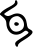
\includegraphics[height=1em]{unown/S}

\includegraphics[height=1em]{unown/B}

\includegraphics[height=1em]{unown/W}

\includegraphics[height=1em]{unown/F}

\includegraphics[height=1em]{unown/O}
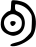
\includegraphics[height=1em]{unown/D}

\includegraphics[height=1em]{unown/J}
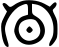
\includegraphics[height=1em]{unown/M}

\includegraphics[height=1em]{unown/B}
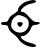
\includegraphics[height=1em]{unown/E}

\includegraphics[height=1em]{unown/F}
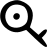
\includegraphics[height=1em]{unown/Q}
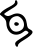
\includegraphics[height=1em]{unown/S}

\includegraphics[height=1em]{unown/F}
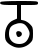
\includegraphics[height=1em]{unown/T}

\includegraphics[height=1em]{unown/J}

\includegraphics[height=1em]{unown/P}
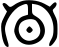
\includegraphics[height=1em]{unown/M}

\includegraphics[height=1em]{unown/F}
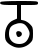
\includegraphics[height=1em]{unown/T}
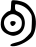
\includegraphics[height=1em]{unown/D}
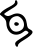
\includegraphics[height=1em]{unown/S}

\includegraphics[height=1em]{unown/J}

\includegraphics[height=1em]{unown/C}

\includegraphics[height=1em]{unown/F}

\includegraphics[height=1em]{unown/N}

\includegraphics[height=1em]{unown/F}

\includegraphics[height=1em]{unown/B}
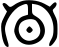
\includegraphics[height=1em]{unown/M}
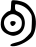
\includegraphics[height=1em]{unown/D}

\includegraphics[height=1em]{unown/P}
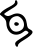
\includegraphics[height=1em]{unown/S}
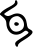
\includegraphics[height=1em]{unown/S}

\includegraphics[height=1em]{unown/F}

\includegraphics[height=1em]{unown/P}

\includegraphics[height=1em]{unown/K}
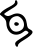
\includegraphics[height=1em]{unown/S}

\includegraphics[height=1em]{unown/C}

\includegraphics[height=1em]{unown/V}
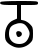
\includegraphics[height=1em]{unown/T}

\includegraphics[height=1em]{unown/U}

\includegraphics[height=1em]{unown/P}
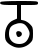
\includegraphics[height=1em]{unown/T}

\includegraphics[height=1em]{unown/N}
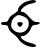
\includegraphics[height=1em]{unown/E}

\includegraphics[height=1em]{unown/F}

\includegraphics[height=1em]{unown/H}
\includegraphics[height=1em]{unown/N}
\includegraphics[height=1em]{unown/B}
\includegraphics[height=1em]{unown/J}
\includegraphics[height=1em]{unown/M}
\includegraphics[height=1em]{unown/Z}
\includegraphics[height=1em]{unown/U}
\includegraphics[height=1em]{unown/F}
\includegraphics[height=1em]{unown/S}
\includegraphics[height=1em]{unown/F}
\includegraphics[height=1em]{unown/H}
\includegraphics[height=1em]{unown/B}
\includegraphics[height=1em]{unown/M}
\includegraphics[height=1em]{unown/P}
\includegraphics[height=1em]{unown/V}
\includegraphics[height=1em]{unown/O}
\includegraphics[height=1em]{unown/B}
\includegraphics[height=1em]{unown/D}
\includegraphics[height=1em]{unown/B}
\includegraphics[height=1em]{unown/S}
\includegraphics[height=1em]{unown/U}
\includegraphics[height=1em]{unown/B}
\includegraphics[height=1em]{unown/F}
\includegraphics[height=1em]{unown/T}
\includegraphics[height=1em]{unown/Q}
\includegraphics[height=1em]{unown/F}
\includegraphics[height=1em]{unown/D}
\includegraphics[height=1em]{unown/J}
\includegraphics[height=1em]{unown/B}
\includegraphics[height=1em]{unown/M}
\includegraphics[height=1em]{unown/Q}
\includegraphics[height=1em]{unown/P}
\includegraphics[height=1em]{unown/S}
\includegraphics[height=1em]{unown/I}
\includegraphics[height=1em]{unown/B}
\includegraphics[height=1em]{unown/D}
\includegraphics[height=1em]{unown/F}
\includegraphics[height=1em]{unown/S}
\includegraphics[height=1em]{unown/N}
\includegraphics[height=1em]{unown/F}
\includegraphics[height=1em]{unown/G}
\includegraphics[height=1em]{unown/F}
\includegraphics[height=1em]{unown/M}
\includegraphics[height=1em]{unown/J}
\includegraphics[height=1em]{unown/A}
}

\vspace{5cm}

\begin{flushright}%
\begin{minipage}{0.7\textwidth}%
        \begin{flushright}%
                {\noindent A la sonrisa eterna de mi hija María Isabel.\\
                A mi familia que siempre me ha ayudado en los momentos más difíciles.\\
                A todas aquellas personas que han contribuido en el desarrollo de las herramientas de código 
		libre con las que desarrolle el presente trabajo, especialmente a los desarrolladores de 
		\LaTeX y Vim.\\
                A todas las personas que han inspirado y entretenido mi vida, especialmente Eiichiro Oda y 
		Yoshihiro Togashi.\\}
        \end{flushright}
\end{minipage}
\end{flushright}

\vspace{3.5cm}

\clearpage % Salto de página
\section*{AGRADECIMIENTOS}

\begin{singlespace}
El autor del presente trabajo de investigación expresa sus agradecimientos:

A Ivan Andres Blanco Polania, por su valioso aporte como director del presente trabajo.

A la Universidad del Tolima, IDEAD y el programa Maestría en Pedagogía y Mediaciones Tecnológicas por su apoyo 
logístico.

A la docente de la institución Ciudad Luz en Ibagué, Gloriset García Mejia por su colaboración y disposición 
durante todo el desarrollo de la presente investigación.

A mi CIPA 6 que colaboraron con su granito de arena en la elaboración y culminación de este proyecto.

A todas las personas en su mayoría anónimas que con sus colaboraciones desinteresada en plataformas como 
stackoverflow o youtube, ayudan personas sin esperar nada a cambio, especialmente a Antonio Leiva 
\end{singlespace}


\clearpage % Salto de página
\section*{Resumen}

\begin{singlespace}
El siguiente proyecto surge de la necesidad de brindar una estrategia didáctica mediada por una aplicación 
móvil para el seguimiento y motivación de las actividades en el aula \cite{SAILER2017371, DAROCHASEIXAS201648}, 
con el objetivo de promover el desarrollo de buenos hábitos de estudio y aumentar el éxito en la terminación 
de actividades por parte de los estudiantes, bajo este contexto, el presente proyecto probará un enfoque 
interactivo del proceso de aprendizaje diseñando y probando una herramienta que involucra elementos de 
gamificación y narración de historias en forma de juegos de rol \cite{rauscher2021comics}.

Para el desarrollo del presente trabajo se construye una tecnología de software de nombre CALINA (en idioma 
Pijao significa Amigo, disponible para su descarga en 
\url{https://play.google.com/store/apps/details?id=co.edu.ut.jrbustosm.calina}), que media el progreso de las 
actividades estudiantiles haciendo uso de técnicas de gamificación y juegos de rol, con el fin de promover la 
apropiación de competencias en cuanto a aprender a aprender y lograr así un desarrollo integral de quien 
consolida un proceso mediado por la aplicación \cite{tornero2016ideas, molina_reconfiguracion_2021}, 
fomentando en los estudiantes la responsabilidad en la ejecución de actividades y el trabajo en equipo 
\cite{XU2017}.

El uso extensivo de técnicas de gamificación permite que el estudiante se encuentre motivado a explorar y 
continuar las actividades propuestas encontrando satisfacción en sus propias conquistas y logros 
\cite{Danka2020, MULLINS2020304}, y al poder ayudar a sus compañeros para que alcancen los mismos objetivos 
que tienen en común promueve valores de unión y solidaridad en el grupo \cite{DING20191}, adicionalmente, el 
planteamiento de actividades bajo un esquema de narración de historias y juegos de rol enriquece contextos 
aburridos del aula estimulando, inspirando y motivando a los estudiantes, especialmente si la historia está en 
concordancia con sus intereses personales lo que interioriza las competencias propuestas 
\cite{8190501, Young2015199}. 

En cuanto al desarrollo metodológico del presente proyecto, presenta dos etapas, una primera del desarrollo de 
la aplicación, implementada inicialmente usando un método de cascada seguido por uno en base a prototipos para 
la construcción del software, y el modelo MAP (Mecánicas, Atributos y Principios) para la adquisición de 
requisitos en cuanto a gamificación \cite{CECHELLA2018}, y una segunda etapa de verificación de tipo 
cualitativo que implementa un diseño cuasi experimental, en el que se van a estudiar la influencia de la 
``gamificación'' y ``juegos de rol'' en los estudiantes desde la perspectiva del docente, para esto, se aplica 
las diferentes estrategias sobre tres grupos diferentes manejados por un único profesor, cada grupo con su 
propia estrategia, (1) grupo de control (2) grupo con gamificación y (3) grupo con gamificación + juego de rol, 
cada uno con dos replicas que consta de sesiones cortas de 30 a 45 minutos. 

La pregunta de investigación radica en que tanto la gamificación como los juegos de rol afectan las emociones 
de los estudiantes \cite{MULLINS2020304}, afectando su motivación y asimilación de las competencias 
propuestas, por lo que se plantean dos instrumentos para su verificación, (1) La aplicación CALINA en si como 
instrumento de medición para hacer seguimiento de las actividades y (2) entrevista no estructurada
al inicio y final de la investigación al docente de la asignatura. 

Finalmente, lo que se pretende con esta investigación es hacer reflexión de como cambiar esquemas de 
aprendizaje, puede brindar a los estudiantes motivaciones intrínsecas (deseo hacerlo) en lugar de las 
motivaciones extrínsecas que suelen darse al estudiante (lo hago por la nota), esto con el fin de generar los 
hábitos de trabajo necesarios en esforzarse para culminar y continuar con algo que deseo hacer, en lugar del 
típico esquema de esforzarse con el fin de superar algo que el profesor desea que haga.
\end{singlespace}

\uline{Palabras clave:} gamificación, narración de historias, story telling, aplicación móvil, juegos de Rol, RPG

%\section*{Abstract}

%\begin{singlespace}
%\end{singlespace}

%\uline{Keywords:} gamification, story telling, mobile application, Role Playing, RPG


\clearpage % Salto de página

% TABLA DE CONTENIDOS - ÍNDICE
% ------------------------------------------------------------------------------
\fancypagestyle{plain}{         % ENCABEZADO PARA LA PRIMERA PÁGINA DE LAS TABLAS DE CONTENIDO
  \rhead{\thepage}
}  
% ------------------------------------------------------------------------------
\tableofcontents
\listoftables
\listoffigures
\clearpage % Salto de página

\pagenumbering{arabic}          % INICIAR NUMERACIÓN

% ------------------------------------------------------------------------------
\pagestyle{fancy}               % ENCABEZADO Y PIE DE PÁGINA PARA EL DOCUMENTO
\fancyhf{}
\rhead{\thepage}
\lhead{\leftmark}
\rfoot{\autordeldocumento}
\lfoot{\titulocortotesis}
\renewcommand{\headrulewidth}{1pt}
\renewcommand{\footrulewidth}{1pt}
% ------------------------------------------------------------------------------

% Autor: Jose Ricardo Bustos Molina
%        Universidad del Tolima
%        jrbustosm@ut.edu.co
%
\section{Introducción}

\subsection{Planteamiento del problema de investigación}	

En el estudio ``Factores asociados al desempeño académico en la  prueba saber 3°, 5° y 9° - 2012'' realizado 
por \citeA{ICFES_2018}, el gobierno nacional presenta la necesidad de mitigar o mejorar en diversos factores 
que influencian directamente el rendimiento escolar, entre varios mencionados las estrategias de aprendizaje y 
el autoconcepto académico, son dos factores que están estrechamente relacionados con disminuir la falta de 
motivación en los estudiantes.

En el día a día del ejercicio docente en Colombia es un hecho, que numerosos estudiantes de secundaria se 
encuentran en un estado donde presentan un bajo deseo en realizar sus tareas académicas, es esta ausencia de 
motivación académica que puede generar sentimientos de frustración y descontento, afectando su productividad y 
el bienestar de ellos mismos \cite{Legault2006-af}. Aunque la motivación académica siempre ha recibido mucha 
atención por parte de los propios docentes, no se ha prestado suficiente atención a las razones por la falta 
de esta, ya que las causas de su carencia es en sí mismo un proceso muy complejo, que no es tanto una ausencia 
de motivación externa hacia el estudiante, si no que incluye un amplio campo de necesidades internas no 
satisfechas en los mismos estudiantes y su entorno.

Es esta naturaleza multidimensional de la desmotivación académica la que explica el comportamiento de los 
estudiantes, y es descrita por \citeA{deci1985intrinsic}, quienes con su modelo de la teoría de 
autodeterminación listan cuatro razones: sus creencias sobre su propia capacidad, las creencias sobre el 
esfuerzo, el valor que se le da a las tareas académicas y las características de las tareas académicas en sí. 

Por lo que los estudiantes que experimentan una situación donde sus capacidades o esfuerzo estén disminuidas
creerán a priori que su situación es permanente y que no hay nada que puedan hacer al respecto, asumiendo 
erróneamente que son los factores externos quienes controlan su destino, experimentando una pérdida de control 
y una sensación general de impotencia. Es por esto, que los esfuerzos docentes para motivar deben ir 
encaminados a aumentar en los estudiantes esta confianza en sus propias habilidades y el esfuerzo, para tener 
éxito en la culminación de su propio currículo.

Por otro lado, el valor otorgado a las actividades académicas esta directamente relacionado con los deseos de
los estudiantes de abandonar o continuar con ellas, es por esto que es necesario que los estudiantes y sus 
seres queridos (familia), valoren abiertamente el éxito académico. Los estudiantes necesitan identificarse con 
estas tareas las cuales requieren tiempo y esfuerzo. En otras palabras, Si los estudiantes valoran lo que 
están haciendo, es probable que se comprometan.

Finalmente las tareas escolares deben ser inspiradoras e interesantes, y los estudiantes deben sentirse 
identificados para realizarlas. Es por esto, que la percepción de los estudiantes a actividades poco 
interesantes, aburridas, o monótonas deben ser reexaminadas en un intento de hacerlas más atractivas. 
Adicionalmente, la importancia que los docentes brinden a sus estudiantes la información y la 
retroalimentación necesaria y oportuna, para impulsar la motivación académica en sus estudiantes.

\subsection{Justificación del problema de investigación}

Hoy en día, uno de los mayores retos para los docentes es lograr construir entornos pedagógicos efectivos y 
atractivos para los estudiantes. Según \citeA{AURA2021101728} gracias a la digitalización de la vida cotidiana 
y una creciente inmigración tanto física como digital, los grupos de estudiantes no solo son cada vez más 
heterogéneos (en términos de raza, género y religiones), sino que sus intereses tanto individuales como de 
colectivo hacen que su capacidad de atención sea disminuida significativamente ya que lo visto en su escuela 
no se ajusta a sus gustos.

Es así como en los últimos años con el aumento en el uso por parte de la comunidad educativa de las redes 
sociales, las plataformas de vídeos y la difusión generalizada de juegos, se ha vuelto casi indispensable para 
los docentes utilizar algunas de las mismas tecnologías que le interesan a los estudiantes para con ellas 
crear entornos de aprendizaje interesantes, atractivos y familiares. Por lo que realizar acciones para mejorar 
el intereses en el aprendizaje e inspirar una enseñanza más apropiada juega un papel importante para los
modelos de aprendizajes modernos \cite{XU2017}. Creando la necesidad de realizar un aprendizaje activo como 
una actividad cotidiana en el aula, lo que requiere que los estudiantes hagan algo más que escuchar y tomar 
notas \cite{8190501}.

%GAMIFICACION
Según \citeA{KUSUMA2021886} al aumentar la motivación también es posible mejorar el rendimiento escolar. Para 
poder lograr este incremento en la motivación escolar es posible aplicar estrategias que usen gamificación, 
concretamente, el desarrollo de prácticas para involucrar y estimular a los estudiantes en el proceso de 
aprendizaje, así como para mejorar su experiencia en el aula \cite{SBIE8805}.

De igual manera \citeA{duran2019}, definen que ``a través del juego se enfrenta el individuo a diferentes 
desafíos y experiencias que tienen que superar aprendiendo de sus experiencias'' es así como la gamificación 
brinda posibilidades en la automotivación, la inquietud por el saber, y la relevancia del juego para 
aplicarlos en la educación, logrando así, un mayor grado de participación en el estudiante y opciones de 
mejora en su rendimiento escolar. Por lo que, el juego se convierte en uno de los medios más poderosos que 
tienen los niños para aprender nuevas habilidades y conceptos a través de su propia experiencia.

Se han realizado estudios sobre el uso de gamificación en la enseñanza y el aprendizaje, y se ha observado la 
influencia positiva de este recurso en áreas como la motivación, el compromiso y el aprendizaje de los 
estudiantes \cite{DING20191}. Sin embargo, las estrategias basadas en gamificación no siempre dan como 
resultado experiencias positivas, existiendo estudios donde no hay ningún efecto o incluso reportando efectos 
negativos, por lo que, un diseño meticuloso contribuye en gran medida al éxito de un proceso que usa este tipo
de técnicas \cite{DING20191}.

%NARRACION
Por otro lado, para este trabajo es indispensable considerar la narrativa como una herramienta que afecta
directamente a los sentidos y emociones de los estudiantes, favoreciendo o afectando el aprendizaje, al 
ofrecer mediante historias la posibilidad de contextualizar las enseñanzas. La narrativa permite unir ideas 
sueltas dentro de las actividades en clase, lo que facilita el recuerdo, la asociación y la transferencia de 
conocimiento \cite{tornero2016ideas}.

Sin embargo, según \citeA{Young2015199} la investigación sobre el papel de la narrativa en los juegos y en el 
aprendizaje en el aula está lejos de ser concluyente, pero son un determinante central del aprendizaje 
humano, ya que la narrativa es el mecanismo a través del cual los humanos construyen la realidad y dan sentido 
al mundo que los rodea. Es por esto que el uso de narrativas y cómo estas pueden apoyar la implementación de 
la gamificación fomentando y desarrollando la creatividad, el interés y apropiación en el aula, es un campo
de estudio que debe ser estudiado y evaluado.

%RPG
Finalmente, el uso propuesto de elementos de juegos de rol (RPG) clásicos es con el fin de proporcionar una 
estrategia integrada y de múltiples frentes para involucrar a los estudiantes, que sirva de elemento de 
cohesión entre la gamificación, narrativa y competencia a aprender, logrando transmitir la información de
una forma interesante para alentarlos a crecer y mejorar.

\subsection{Objetivos de la investigación}

\subsubsection{Objetivo general}

Construir y evaluar una aplicación gamificada para móviles que usa juegos de rol para el desarrollo de 
actividades escolares

\subsubsection{Objetivos específicos}

\begin{itemize}
\item Identificar las necesidades que presentan los estudiantes, para el buen desarrollo o culminación de sus
actividades escolares.

\item Seleccionar las estrategias adecuadas de gamificación y de juegos de rol adecuadas de acuerdo al 
contexto para su aplicación en un proceso educativo.

\item Evaluar mediante instrumentos de investigación para dimensionar la motivación el modo en que las 
técnicas de gamificación y juegos de rol afectan el comportamiento de los estudiantes.
\end{itemize}

\subsection{Pregunta de investigación}

¿En que medida afecta el uso de estrategias gamificadas y basadas en juegos de rol a la motivación y la
culminación de actividades en los estudiantes?

\subsection{Categorías de investigación}

\begin{table}[ht]
\caption{Categorías de Investigación}
\label{tab:catinv}
\small
\begin{center}
	\begin{tabular}{ p{40mm} p{30mm} p{30mm} p{40mm}}
\toprule
\textbf{Pregunta} & \textbf{Categorías} & \textbf{Subcategorías} & \textbf{Técnicas} \\ 
\midrule
¿Cómo afecta la gamificación en la motivación y culminación de actividades? & Gamificación & Mecánicas 
	\newline Dinámicas \newline Diégesis & Aplicación CALINA \newline Implementación de estrategia 
	gamificada\\
¿Cómo afecta los juegos de rol en la motivación y culminación de actividades? & Narración de Historias & 
	Juegos de Rol & Aplicación CALINA \newline Implementación de juego de rol\\
¿Cómo medir el grado de motivación en un estudiante? & Teorías Motivación & Autodeterminación \newline 
	Culminación \newline Cooperativo \newline Retroalimentación \newline Individualización & Aplicación 
	CALINA \newline Observación participante ajena\newline Diseño encuesta\\
\bottomrule
\multicolumn{4}{l}{\footnotesize Fuente: de elaboración propia.}\\
\end{tabular}
\end{center}
\end{table}


\clearpage % Salto de página
% Autor: Jose Ricardo Bustos Molina
%        Universidad del Tolima
%        jrbustosm@ut.edu.co
%
\section{Antecedentes}

Para investigar el estado académico actual acerca de la influencia de la gamificación y los juegos de rol 
sobre la motivación de los estudiantes, se realizó una revisión sistemática de literatura utilizando las bases 
de datos Science direct, Springer link, Scopus, Oxford academic, Google scholar, EBSCO y el gestor de la 
biblioteca de la Universidad del Tolima y demás universidades con programas de maestría en el área de 
educación, como se muestra en el modelo de la Figura \ref{img:busqueda}. Para implementar esta búsqueda se 
usó como fuente inicial la cadena de búsqueda:

\begin{center}\ttfamily\sbox{0}{a}    % Poner tipo de fuente
\begin{minipage}{64\wd0}              % página de 64 caracteres
\begin{verbatim}
(gamif* OR rol* game) AND (motivation) OR (gamif* AND rol* game)
      LIMIT(10 year), AREA(social sciences AND psychology)
\end{verbatim}
\end{minipage}
\end{center}

\begin{figure}[ht]
\caption{Modelo búsqueda sistemática bibliografía}
\label{img:busqueda}
\centering
\begin{tikzpicture}[
		every node/.append style={draw=gray!80,align=center,minimum width=90pt,very thin}
  	]
	\node (I) at (-3.5,-1.5) {
		\textbf{\small Inicio}
	};
	\node (CB) at (-3.5,0.5) {
		\textbf{\small Cadena de Búsqueda}\\{\scriptsize (gamif* OR rol* game) AND}\\
		{\scriptsize (motivation) OR (gamif* AND rol* game)}\\
		{\scriptsize LIMIT(10 year),}\\
		{\scriptsize AREA(social sciences AND psychology)}
	};
	\node (BD) at (-3.5,4) {
		\textbf{\small Base de Datos}\\{\scriptsize Science direct, Springer link, Scopus,}\\{\scriptsize Oxford Academic, google scholar, EBSCO, UT}
	};
	\node (WC) at (2.7,0.5) {
		\textbf{\small Nubes de Palabras}\\ \includegraphics[width=.3\textwidth]{img/keywords_count_full}
	};
	\node (E) at (2.7,4) {
		\textbf{\small Descarga Articulo/Metadatos}\\{\scriptsize Título, Autores, Resumen, Año,}\\{\scriptsize Palabras Clave, Tipo, Publicación}
	};
	\node (R) at (5.7,5.5) {
		\textbf{\small Artículos recomendados (IA)}
	};
	\node (C) at (8,4) {
		\textbf{\small Clasificación (Jabref)}\\{\scriptsize Review, Gamificación, Narración,}\\{\scriptsize RPG, Motivación, Misceláneo}
	};
	\node (A) at (8,2.3) {
		\textbf{\small Anotación}
	};
	\node (An) at (8,0) {
		\textbf{\small Análisis}\\ \includegraphics[width=.2\textwidth]{img/teoriasYmodelos.sort}
	};
	\draw[-triangle 90] (I) edge (CB);
	\draw[-triangle 90] (CB) edge (BD);
	\draw[-triangle 90] (BD) edge (E);
	\draw[-triangle 90] (E) edge (WC);
	\draw[-triangle 90] (WC) edge (CB);
	\draw[-triangle 90] (E) edge (C);
	\draw[-triangle 90] (C) edge (A);
	\draw[-triangle 90] (A) edge (An);
	\draw[-triangle 90,dashed] (E) edge (R);
	\draw[-triangle 90,dashed] (R) edge (C);
\end{tikzpicture}


{\footnotesize Fuente: de elaboración propia.}
\end{figure}

En la búsqueda sistemática se limitó a metadatos, que incluían títulos, resúmenes y palabras clave. Se realizó 
el análisis de nuevos términos de búsqueda usando nubes de palabras generadas a partir de los resúmenes y las 
palabras claves de los artículos seleccionados (ver Figura \ref{img:nube}), para modificar las respectivas 
cadenas de búsqueda y volver a repetir el proceso usando nuevos términos. 

\begin{figure}[ht]
  \caption{Nubes de palabras generadas}
  \label{img:nube}
  \centering
  \subfloat[A partir de los títulos y resúmenes]{
    \includegraphics[width=0.45\textwidth]{abstracts_count_lemmatize}\label{img:nubef1}
  }
  \hfill
  \subfloat[A partir de las palabras claves]{
    \includegraphics[width=0.45\textwidth]{keywords_count_full}\label{img:nubef2}
  }
  \\
  {\footnotesize Fuente: de elaboración propia.}
\end{figure}

Si bien existe una cantidad sustancial de investigación en gamificación, solo una minoría de estas 
publicaciones utiliza juegos de rol o la narración de historias como un complemento. En total, se encontraron
76 publicaciones que cumplían los parámetros deseados, 29 del orden regional y 47 del orden internacional, 
donde 54 documentos tratan sobre gamificación, 13 tratan de la narración de historias, 14 tratan el tema de 
juegos de rol y 7 sobre teorías de motivación, de estos trabajos, hay 10 que combinan las estrategias de 
juegos de rol con gamificación y 9 que mezclan la estrategia de narración de historias con la gamificación. 
Esto se puede ver resumido en la Figura \ref{img:catbib}.

En cuanto al tipo de publicación encontrada son 30 artículos, 26 tesis de maestría, 11 libros, 6 artículos de 
conferencias, y 3 capítulos de libro. Además, 68 de estas publicaciones son de los últimos 10 años y 8 de años 
anteriores.

Por otra parte, es importante resaltar que de los 54 estudios sobre gamificación, 52 estudios arrojaron 
resultados motivacionales o relacionados con el desempeño o la motivación positivos o ligeramente positivos, 
mientras que dos estudios encontraron resultados mixtos \cite{DING20191, PRESTOPNIK2015492}.

\begin{figure}[ht]
\caption{Resumen categorías de bibliografía}
\label{img:catbib}
\centering
\begin{tikzpicture}[pattern color=lightgray, pattern=north east lines]
	\scope
	\clip (-3,0) circle (2);
	\fill (0,0) circle (2);
	\endscope
	\scope
	\clip (3,0) circle (2);
	\fill (0,0) circle (2);
	\endscope
	\draw (-3,0) circle (2) (-3,2.4)  node {Juegos de Rol} (-3,0)  node {\LARGE 4};
	\draw (-1.5,0)  node {\Large 10};
	\draw (3,0) circle (2) (3,2.4)  node {Narración} (3,0)  node {\LARGE 4};
	\draw (1.5,0)  node {\Large 9};
	\draw (0,0) circle (2) (0,2.4)  node {Gamificación} (0,0)  node {\LARGE 35};
	\draw (7,0) circle (1.5) (7,1.9)  node {Otras} (7,0)  node {\LARGE 14};
	\draw (-6,-2.5) rectangle (9,3);
	\draw (7,3.4) node {H=76 publicaciones};
\end{tikzpicture}

\\
{\footnotesize Fuente: de elaboración propia.}
\end{figure}

\pagebreak

Adicional a esto, se usaron los textos completos para realizar un conteo de las teorías o modelos 
(psicológicos, pedagógicos o de aprendizaje) mencionadas en los estudios, mostrando predominancia en cuanto a 
dos teorías en particular: teoría de la autodeterminanción y teoría de reforzamiento conductual, 
como se puede ver en la Figura \ref{img:nubeteorias}.

\begin{figure}[H]
  \caption{Nubes de palabras generadas para teorías y modelos}
  \label{img:nubeteorias}
  \centering
  \includegraphics[width=0.8\textwidth]{teoriasYmodelos.sort}
  \\
  {\footnotesize Fuente: de elaboración propia.}
\end{figure}

\subsection{Antecedentes regionales del uso de estrategias de gamificación o juegos de rol en educación}

En el contexto del departamento del Tolima y con el objetivo de establecer antecedentes sobre gamificación, se 
presentan adicionalmente investigaciones en contexto local que usan la lúdica como eje fundamental del 
aprendizaje, en cuanto al contexto nacional se hace especial énfasis en trabajos de maestría que desarrollen 
la categoría de gamificación y el uso de juegos de Rol, mas no el desarrollo de juegos serios. Por lo tanto,
se implemento una búsqueda sistemática para el descubrimiento de tesis a nivel de maestría o doctorado, en los
diferentes motores de búsqueda implementados en los portales de bibliotecas de cada Universidad, obteniendo un 
total de 25 tesis todas ellas a nivel de maestría, de 14 instituciones diferentes las cuales se pueden ver 
resumidas en la tabla \ref{tab:resumenlocal}.

\begin{table}[!htb]
\caption{Resumen tesis de maestría gamificación/juego de roles a nivel nacional}
\label{tab:resumenlocal}
\begin{center}
\footnotesize
\begin{tabular}{ p{50mm} p{50mm} p{15mm} c}
\toprule
	\textbf{Universidad} & \textbf{Programa(s)} & \textbf{Ciudad} & \textbf{Cantidad}\\ 
\midrule
	Pontificia Universidad Javeriana & Maestría en Ingeniería Electrónica & Bogotá & 1\\
	Universidad Cooperativa de Colombia & Maestría en Educación & Bogotá & 1\\
	Universidad de Antioquia & Maestría en Educación & Medellín & 1\\
	Universidad de la Costa & Maestría en Educación & Barranquilla & 1\\
	Universidad de los Andes & Maestría en Educación & Bogotá & 1\\
	Universidad de Santander UDES & Maestría en Tecnologías Digitales Aplicadas a la Educación & Bogotá & 
	1\\ 
	Universidad del Tolima & Maestría en Educación & Ibagué & 3\\
	Universidad Icesi & Maestría en Educación & Santiago de Cali & 2\\
	Universidad Nacional de Colombia sede Bogotá & Maestría en Ingeniería – Ingeniería de Sistemas y 
		Computación / Maestría Enseñanza de las Ciencias Exactas y Naturales & Bogotá & 2\\
	Universidad Nacional de Colombia sede Medellín & Maestría Enseñanza de las Ciencias Exactas y 
		Naturales & Medellín & 4\\
	Universidad Pedagógica Nacional & Maestría Tecnologías de la Información Aplicadas a la Educación & 
		Bogotá & 1\\
	Universidad Pontificia Bolivariana & Maestría en Educación & Medellín & 1\\
	Universidad Tecnológica de Bolívar & Maestría en Educación/Maestría en Gestión De La Innovación & 
		Cartagena &  4\\
	UPTC, Universidad Pedagógica y Tecnológica de Colombia & Maestría en TIC Aplicadas a las Ciencias de 
		la Educación & Duitama & 1\\
\bottomrule
	\multicolumn{4}{l}{\footnotesize Fuente: de elaboración propia.}\\
\end{tabular}
\end{center}
\end{table}

En el presente estudio, no se pudo evidenciar localmente trabajos sobre gamificación a nivel de maestría o 
doctorado, sin embargo, si se encuentran tres trabajos relacionados al tema sin que este sea su eje principal,
por ejemplo, \citeA{barragan2015}, en su trabajo ``Square Game como apoyo del proceso de evaluación de la 
geometría en el segundo grado de básica primaria de la región Alto Magdalena - Colombia'', que plantea el 
desarrollo de un juego serio basado en Tangram para simplificar procesos cognitivos en la enseñanza de la 
geometría, consiguiendo un aprendizaje significativo en el aprendizaje de figuras geométricas básicas en los 
estudiantes.

Adicional a esto, \citeA{lobo2015} en su proyecto ``Estrategia metodológica basada en la actividad lúdica para 
el desarrollo del pensamiento variacional en estudiantes de 8º grado que cursan la asignatura matemática en la 
institución educativa rural San Joaquín del municipio de Santa María-Huila'' quienes proponen una estrategia 
metodológica basada en la lúdica para potenciar el desarrollo del pensamiento matemático (propiedades, 
lenguaje algebraico, operaciones y resolución de problemas) en los estudiantes y un estudio cualitativo de su 
implementación.

Finalmente, \citeA{garcia2014}, en su estudio ``Uso pedagógico del celular en el aula'', cuyo propósito fue 
estimar la tenencia de teléfonos celulares por parte de estudiantes y profesores, mostrándonos un escenario 
idóneo para propiciar eventos de enseñanza-aprendizaje usando los móviles como medio de mediación.

En cuanto al contexto nacional, son varios los que hacen uso extensivo de la gamificación como estrategia para
el aprendizaje, por ejemplo \citeA{Mera-Paz_2016} realiza una reflexión sobre la gamificación como estrategia 
para el fortalecimiento del pensamiento algorítmico en el programa ingeniería de sistemas de la Universidad 
Cooperativa de Colombia sede Popayán, y \citeA{MORENO2015} quienes crean y evalúa una estrategia didáctica 
gamificada implementada en un ambiente virtual para los cursos de pre-cálculo de la Universidad Nacional de 
Colombia, mostrando un incremento en el desempeño académico y en el porcentaje de aprobación, al tiempo que
una disminución en el abandono estudiantil.

De acuerdo con la búsqueda realizada de tesis a nivel de maestría en Colombia, los diferentes estudios se 
pueden clasificar en tres grandes grupos: orientados a la educación escolar, a la participación ciudadana y 
bajo un contexto empresarial. Sin embargo, el número de trabajos de estos dos últimos grupos es mas bajo (4 
trabajos en total), respecto al uso de gamificación o juegos de rol en el ambiente educativo, que es donde se 
encuentra el grueso de los esfuerzos de investigación en los diferentes programas de maestría (18 en total), 
incluyendo dos trabajos que usan los juegos de rol en conjunto con la gamificación como estrategia de 
enseñanza.

Anudando a lo anterior, el uso de estrategias gamificadas o juegos de rol en la educación, se pudo evidenciar
su uso en la enseñanza del área de ciencias naturales (9 trabajos), ciencias humanas (3 trabajos), tecnología 
(1 trabajo), idioma extranjero (2 trabajos), matemáticas (2 trabajos) y un estudio genérico. A continuación, a 
manera de resumen, se muestra en la tabla \ref{tab:bioanotada} la bibliografía anotada anteriormente descrita 
y clasificada.

\begin{center}
\footnotesize
\begin{longtable}{ p{25mm} p{50mm} p{75mm} }
	\caption{Bibliografía anotada de tesis de maestría en Colombia, tema: Gamificación y Juegos de Rol}
	\label{tab:bioanotada} \\

	\toprule
	\textbf{Autores} & \textbf{Título} & \textbf{Anotación}\\
	\midrule
	\endfirsthead
	
	\toprule
	\textbf{Autores} & \textbf{Título} & \textbf{Anotación}\\
	\midrule
	\endhead

	\midrule
	\multicolumn{3}{r}{{Continúa en la siguiente página\dots}} \\
	\bottomrule
	\endfoot

	\bottomrule
	\multicolumn{3}{l}{\footnotesize Fuente: de elaboración propia.}\\
	\endlastfoot

\citeA{Albornoz2021} & Estrategia Didáctica Basada en la Gamificación para el Fortalecimiento de las 
Habilidades Investigativas en Estudiantes de Grado Sexto (\textbf{Universidad de Santander UDES}) & Se 
desarrolla un trabajo que mediante un diseño de un curso virtual que usa gamificación fortalezca las 
habilidades investigativas en estudiantes de grado sexto, estudio con enfoque \uline{cualitativo}, encontrando 
una mejora a partir de la implementación de la estrategia didáctica gamificada respecto al grupo de control.\\
\citeA{Arias2021} & La gamificación como estrategia que contribuye al desarrollo del uso comprensivo del 
conocimiento científico mediante la enseñanza del sistema digestivo humano (\textbf{Universidad Nacional de Colombia}) 
& Estrategia gamificada implementada en estudiantes de grado quinto para el aprendizaje del sistema digestivo, 
usando un enfoque \uline{cualitativo} con una metodología de \uline{investigación-acción}, concluyendo que 
esta contribuye de una forma positiva a la comprensión por parte de los estudiantes, pudiendo evidenciar 
exitosamente el interés en los estudiantes\\
\citeA{Arias2012} & Uso de un juego de rol como herramienta de motivación en la enseñanza de la química 
(\textbf{Universidad Nacional de Colombia}) & Muestra el uso de un juego de rol como estrategia para aumentar 
la motivación en la enseñanza de la química orgánica en un curso de educación superior, usando elementos de 
\uline{aprendizaje basado en problemas y colaborativo}, encontrando resultados positivos en cuanto a 
motivación, participación y aprendizaje, adicionalmente mejorando la relación docente-estudiante.\\
\citeA{betancur2018} & La literatura infantil y juvenil, desde la gamificación: un escenario posible para la 
formación literaria en la básica primaria (\textbf{Universidad de Antioquia}) & Investigación que busca 
fortalecer la formación literaria en estudiantes del grado tercero, usando técnicas gamificadas y un enfoque 
\uline{cualitativo} en la investigación, encontrando que la implementación de este tipo de estrategias 
favorece el desarrollo de diversas competencias lingüísticas y comunicativas en los estudiantes, mejorando
los hábitos lectores, y un incrementó en el interés frente a la literatura y el proceso lector.\\
\citeA{Buitrago2021} & Estrategia de gamificación para la enseñanza y evaluación de la estructura atómica en 
la educación básica en el contexto rural (\textbf{Universidad Nacional de Colombia}) & Plantea una estrategia 
gamificada usando el \uline{aprendizaje basado en problemas}, para la enseñanza de la estructura de los átomos 
en estudiantes de grado sexto, usando un enfoque \uline{cualitativo} y bajo el paradigma critico social 
(modelo de investigación acción educativa), encontrando una mejoría respecto a la actitud por parte de los 
estudiantes, respecto a los tiempos y compromisos en las clases síncronas mediadas por TICs.\\
\citeA{camacho2020} & Estrategia didáctica de gamificación y juego de rol para la promoción de la convivencia 
y la paz en estudiantes de tercero de primaria (\textbf{Universidad Icesi}) & Desarrolla un juego de rol 
gamificado para educar habilidades en la convivencia escolar y la paz, en estudiantes de tercero de primaria. 
Mediante el uso de un enfoque \uline{cualitativo}, se encuentra que la estrategia aportó en el desarrollo 
afectivo emocional de los estudiantes, logrando entretenerlos y estimularlos, fortaleciendo la capacidad de 
diálogo, y la capacidad de generar acuerdos comunes en la resolución de conflictos.\\
\citeA{cano2019} & Un estudio comparado sobre gamificación en dos contextos educativos del área metropolitana 
del valle de aburrá (\textbf{Universidad Pontificia Bolivariana}) & Este trabajo de investigación propone la 
aplicación de una estrategia gamificada en dos instituciones educativas diferentes, el estudio presenta un
enfoque \uline{cualitativo} y con un \uline{diseño cuasiexperimental}, encontrando un impacto positivo en el 
rendimiento académico de los estudiantes, permitiendo encontrar un aumento en los niveles de motivación y
compromiso.\\
\citeA{Cuervo2021} & Evaluación del efecto de la gamificación asistida por computador en la motivación de los 
estudiantes de programación de computadores (\textbf{Universidad Nacional de Colombia}) & Esta investigación 
tiene como propósito dimensionar el efecto que la gamificación en el aprendizaje de programación de 
computadores, en estudiantes de nivel universitario. Para tal fin, se emplea un \uline{enfoque mixto} y a 
través de un estudio \uline{cuasi-experimental}, encontrando un incremento significativo en los niveles 
relacionados con la valoración de tareas, atribuyendo un mayor grado de importancia, utilidad, gusto o 
interés por su realización.\\
\citeA{delahoz2015} & Gamificación para la gestión de la innovación en las organizaciones : caso empresa del 
sector químico de la ciudad de Barranquilla (\textbf{Universidad Tecnológica de Bolívar}) & Se desarrolla un 
proyecto que mediante el \uline{análisis de casos} con un enfoque \uline{cualitativo}, potencia la gestión de 
la innovación en las organizaciones privadas, usando el método de \uline{triangulación de datos} que permite 
analizar un juego construido con el fin estructurar y sistematizar procesos de innovación y liderazgo.\\
\citeA{Duc_Des_2020} & Desarrollo de una estrategia didáctica gamificada mediada por TIC para la enseñanza de 
conceptos de ecología a través de la lectura grado décimo de la educación media en Colombia (\textbf{UPTC, 
Universidad Pedagógica y Tecnológica de Colombia}) & En este trabajo de investigación se desarrolló una 
estrategia didáctica gamificada mediada por TIC, con el objetivo de mejorar la apropiación de conceptos de 
ecología, el estudio se realizó dentro de un enfoque de \uline{investigación mixto}, el impacto de la 
estrategia usada no tuvo impacto en cuanto a la apropiación de conocimientos en ecología, sin embargo, si se 
reporta un incremento en cuanto al cumplimiento de criterios y uso, mostrando una buena aceptación por parte 
de los estudiantes.\\
\citeA{Galeano2016} & El uso de las técnicas de gamificación en la adquisición de vocabulario y el dominio de 
los tiempos verbales en inglés (\textbf{Universidad Pedagógica Nacional}) & El trabajo de investigación busca 
evaluar la incidencia que tiene un videojuego que se apoya en estrategias gamificadas y otro sin técnicas de 
gamificación, para el proceso de adquisición de vocabulario y dominio de los tiempos verbales en inglés, para
el análisis usa un \uline{modelo cuantitativo cuasi-experimental}, encontrando resultados significativos en 
cuanto a mejores resultados del juego gamificado respecto al juego sin gamificación.\\
\citeA{gonzalez2019} & Gamificación ¡Sigamos a Rafael! Sistematización de un experiencia (\textbf{Universidad 
Tecnológica de Bolívar / Corporación Universitaria Minuto de Dios - UNIMINUTO}) & Este trabajo busca el 
fortalecimiento en el aprendizaje de la cultura de la organización Minuto de Dios a través de la 
implementación de un juego basado en la vida de Rafael García Herreros, mediante la metodología 
\uline{pensamiento de diseño}, se concluye que la estrategia gamificada tiene gran aceptación y una influencia 
positiva en los miembros de la corporación.\\
\citeA{Guayara2018} & La gamificación como estrategia de enseñanza en el área de Ciencias Naturales 
(\textbf{Universidad de los Andes}) & Esta investigación propone la utilización de la gamificación como 
estrategia para mejorar la enseñanza de las Ciencias Naturales, planteando el uso de la metodología de 
\uline{Investigación Acción} en dos ciclos de intervención, encontrando diferencias en cuanto a motivación por 
parte de los estudiantes de primaria y de bachillerato, ya que los estudiantes de primaria le dan un valor 
mayor a los puntos asignados en la estrategia, sin embargo, las autoras le dan importancia al uso de 
narrativas como un factor fundamental en la motivación y el compromiso en las actividades.\\
\citeA{Mosquera2020} & Proyecto de aula que contribuya a la enseñanza de la conservación del medio ambiente a 
través de la gamificación (\textbf{Universidad Nacional de Colombia}) & El proyecto de investigación tiene 
como objetivo, crear hábitos usando estrategias que involucran gamificación, para la apropiación en 
conservación del medio ambiente y el desarrollo de competencias científicas, presentando un enfoque 
\uline{cualitativo} que concluye un resultado positivo de la aplicación de estas técnicas en cuanto a los 
temas vistos.\\
\citeA{perez2021} & Estrategia didáctica apoyada en la gamificación para fortalecer la competencia 
comunicativa en el idioma inglés con los estudiantes de grado décimo de la IED Betulia Tena Cundinamarca 
(\textbf{Universidad Cooperativa de Colombia}) & La investigación tuvo como objetivo implementar una 
estrategia didáctica apoyada en gamificación con el fin de fortalecer las competencias en inglés, esta 
investigación tiene una perspectiva \uline{cualitativa} con un alcance \uline{descriptivo evaluativo}, 
abordando el diseño metodológico de \uline{estudio de caso}, encontrando resultados positivos en cuanto a la 
mejora del nivel de inglés por parte de los estudiantes del estudio.\\
\citeA{Restrepo2021} & Estrategia didáctica basada en gamificación para el proceso de enseñanza de la genética 
molecular (\textbf{Universidad Nacional de Colombia}) & El trabajo realiza una \uline{revisión documental}, la 
cual tiene como objetivo analizar estrategias didácticas basadas en gamificación en la temática de ciencias, y 
acotando la búsqueda a la subcategoría de genética molecular, permitiendo evidenciar los beneficios de la 
implementación de la gamificación en el contexto planteado.\\
\citeA{Laura2015} & Estudio e implementación de mecanismos de privacidad e incentivos para dar soporte a una 
red de sensado participativo de monitoreo de la calidad del aire (\textbf{Pontificia Universidad Javeriana}) & 
Desarrolla un sistema participativo para la recolección de información en calidad de aire, usando la 
gamificación para dar incentivos a la comunidad, aunque se encuentra que los incentivos monetarios presentan 
un mejor indice de éxito, se encuentra que las técnicas de gamificación como sistema de recompensas ofrece una
opción atractiva para los participantes de la red de monitoreo, explotando la necesidad de cumplir metas 
intrínsecas de las personas involucradas.\\
\citeA{rojas2019} & Un sistema gamificado basado en la estrategia de Pólya para el desarrollo de habilidades 
metacognitivas y el logro académico en estudiantes de grado 5°en la resolución de problemas matemáticos de 
operaciones básicas (\textbf{Universidad Pedagógica Nacional}) & La investigación evalúa la estrategia de 
Pólyai en conjunto con gamificación en estudiantes de grado quinto, por medio la metodología tipo 
\uline{mixta} utilizada en el estudio y un \uline{diseño cuasi-experimental} se encuentra resultados 
positivos del uso de gamificación en conjunto con Pólya mejorando los logros en el aprendizaje.\\ 
\citeA{rojas2021} & Ambiente de aprendizaje Gamificado, mediado por las TIC para el fortalecimiento y 
desarrollo de competencias ciudadanas integradoras en estudiantes de grado quinto (\textbf{Universidad Icesi}) 
& La investigación es un \uline{estudio de caso} con \uline{enfoque cualitativo}, basada en la observación y 
descripción de situaciones o acciones que permiten determinar la contribución de la gamificación mediada con
TIC para el fortalecimiento y desarrollo de competencias ciudadanas, mediante el uso de la \uline{observación 
participante y cuestionarios} se puede evidenciar el fortalecimiento de actitudes y valores (ser) a favor de 
la convivencia.\\
\citeA{ruiz2017} & Diseño de un modelo para potencializar la cultura de la calidad en el marco de la NTC ISO 
9001:2015, a través de estrategias de gamificación (\textbf{Universidad Tecnológica de Bolívar}) & El trabajo 
busca lograr que las personas en una empresa adopten y fomenten comportamientos y conductas deseadas en cuanto 
a sistemas de calidad ISO, mediante una \uline{investigación exploratoria} para la implementación de la 
estrategia construida se hacen recomendaciones sobre su uso e implementación\\
\citeA{Salgado2020} & La gamificación como estrategia innovadora en la enseñanza de la física : caso I.E. 
Fulgencio Lequerica Vélez (\textbf{Universidad Tecnológica de Bolívar}) & Mediante una \uline{metodología 
mixta}, se analiza la gamificación como estrategia en la enseñanza de la física de los estudiantes de grado 
10, encontrando que aporta elementos que favorecen el proceso de enseñanza.\\
\citeA{sanchez2018} & La gamificación a través de la plataforma Smartick para mejorar el rendimiento académico 
en matemáticas en estudiantes de la I.E.D. Tercera Mixta de Fundación Magdalena (\textbf{Universidad de la 
Costa}) & El trabajo usa \uline{investigación-acción} para implementar una estrategia de aprendizaje 
gamificada como producto de la reflexión de un grupo docente del departamento de matemáticas, presentando como
resultado del uso y desarrollo de variados estrategias que permiten captar la atención de los estudiantes, 
vigilar las motivaciones explícitas para que no afecte el trabajo de salón y aumentar la motivación junto con 
los estudiantes por el proceso.\\
\end{longtable}
\end{center}

\subsection{Antecedentes internacionales del uso de estrategias de gamificación o juegos de rol en educación}
	
Se realiza una revisión sobre el corpus existente en tres áreas: gamificación y su relación con la motivación,
la gamificación y uso en conjunto con la narración de historias, la narración de historias como estrategia
motivadora.

%-------GAMIFICACIÓN
En cuanto a \textbf{gamificación} los hallazgos de la revisión indican que la mayoría de los estudios se 
centran principalmente en la descripción de los requisitos del usuario para la adaptación de las mecánicas del 
juego \cite{Klock2020}, por ejemplo en el trabajo de \citeA{baldeon2015}, mostrando una experiencia de 
gamificación para aprender fracciones en escuelas  primarias. Sin embargo, se toman en cuenta solo aquellos 
que describan, evalúen o interpreten la modificación de la conducta por parte de esta estrategia, por ejemplo 
\citeA{DING20191}, se plantea el objetivo de evaluar si las gamificaciones se pueden aplicar en las 
discusiones en línea para impulsar la participación estudiantil, teniendo efectos positivos sobre el número de 
comentarios y el rendimiento de los estudiantes en las discusiones en línea, sin embargo, el enfoque fracasó 
en promover el sentido de comunidad por parte de los estudiantes.

Las publicaciones sobre gamificación generalmente muestran resultados positivos, sin embargo hallazgos
como el articulo de \citeA{DING20191} muestran que una estrategia gamificada puede influenciar negativamente
en el comportamiento del estudiante, estos resultados contradictorios pueden ser el resultado de dos factores 
principales: el diseño de gamificación o el diseño de investigación inapropiados.

Por otro lado \citeA{PUTZ2020106392}, realizan un trabajo de investigación para fomentar la retención de 
conocimientos mediante un enfoque de investigación-acción usando gamificación, encontrando que la gamificación 
ejerce un impacto positivo en la retención de conocimientos. Aunque, ellos mencionan que
este estudio se realizó en Austria y debido a las diferencias culturales se podrían presentar otro tipo de
resultados dependiendo del contexto. Esto es concordante con lo expuesto por \citeA{MULLINS2020304} quienes 
revisan un enfoque basado en psicología y neurociencia para examinar los procesos cognitivos y emocionales que
tienen correlación con la gamificación.

Es así, como \citeA{DAROCHASEIXAS201648} evalúan la efectividad de las plataformas gamificadas como estrategia 
para un aumento en la participación y compromiso por parte de los estudiantes, al igual que 
\citeA{Buckley20161162} quienes investigan la relación entre la motivación y la participación en el 
aprendizaje usando juegos en linea y gamificación.


Finalmente \citeA{Danka2020}, sugiere que se deben adaptar las herramientas de evaluación formativa 
motivacional usadas en conjunto con gamificación, como las utilizadas en los juegos de rol multijugador en 
línea (MMORPG), ya que este tipo de evaluación (en lugar de sumativa), puede ser una herramienta educativa 
motivadora adicional que podría hacer que las tasas de finalización de actividades sean más aceptables.

%-------------GAMIFICACIÓN+STORYTELLING

En cuanto al uso de la \textbf{narración de historias} y como esta enriquece el contexto \textbf{gamificado}, 
de acuerdo a la revisión documental realizada se puede afirmar que la narración afecta la gamificación en 
general de forma positiva \cite{articleGiakalaras}. Por ejemplo \citeA{XU2017}, quienes diseñan una estrategia 
de juego de roles con el apoyo de la gamificación para estimular el interés de los alumnos.

Continuando, \citeA{PRESTOPNIK2015492} quienes muestran en su estudio que los estudiantes prefieren 
fuertemente los juegos basados en historias sobre los juegos basados en puntos, y \citeA{trevor2017} quien usa
un tipo de narración no lineal, encontrando un vínculo fuerte entre la narración no lineal con la gamificación
que puede mejorar drásticamente el aprendizaje en la educación en línea.

Es así, como se puede hallar diferentes publicaciones que implementan estas estrategias combinadas, tales 
como, \citeA{TOPIRCEANU201741} quien presenta una plataforma educativa llamada Gamified, que simplifica los 
sistemas educativos y de calificación en las escuelas y universidades basados en juegos de rol, 
\citeA{Cezar2019116} quienes analizan las opiniones de los estudiantes sobre el uso de la gamificación en el
aprendizaje de cálculo utilizando un juego de rol y \citeA{Brieger2013ExploringNC} quien tiene un enfoque mas 
corporativo investigando como usar las estrategias gamificadas en un entorno de comunicación o marca con el 
fin de adaptar el enfoque a cada individuo gracias a elementos tanto de narración, transmedia, como de 
gamificación.

Finalmente se dan pautas de como implementar este tipo de modelo mixto, entre otros 
\citeA{doi:10.1089/cyber.2012.0492} donde identifican características de gamificación atractivas para sitios
web de narración colaborativa, \citeA{SBIE8805} quienes analizan datos obtenidos de una encuesta sobre los 
elementos de juego y narración preferidos por los estudiantes en un contexto educativo, 
\cite{13034670820180801} que propone mirar World of Warcraft (WoW) para encontrar ideas para diseñar 
comunidades en línea novedosas basadas en principios gamificados y \cite{Ntokos2019} quienes proponen un marco 
de diseño para gamificación basado en reglas de videojuegos y juegos de rol.

%------------STORYTELLING
Por último, en cuanto a \textbf{narración de historias} y como esta afecta el comportamiento de los 
estudiantes, \citeA{KUSUMA2021886} investigan cómo un enfoque de aprendizaje basado en juegos de rol influye 
en el logro y la motivación de eventos históricos a través de un entorno de aprendizaje móvil, por lo que el 
juego de rol digital (RPG) se puede utilizar como una herramienta para (apoyar) la enseñanza y el aprendizaje 
en distintas áreas \cite{Nunes2021663}, por ejemplo, en una aplicación con elementos de gamificación y 
narración de historias, para enseñar fundamentos del dogma central de la biología \cite{Ibarra-Herrera2019}.

Anudando a lo anterior \citeA{Gironacci201790} describen un entorno colaborativo de narración de historias 
digitales que utiliza una tableta, un visor de realidad aumentada y un sistema de back-end de minería de datos 
avanzada, \citeA{8190501} quienes analizan el uso de actividades de juego de roles en equipo para simular la 
experiencia de trabajar en un estudio de desarrollo de juegos profesional como un medio para mejorar el 
compromiso y retención de competencias, y finalmente \citeA{AURA2021101728} quienes hacen un estudio para 
examinar una escuela en EEUU haciendo uso de la narración de diversos mundos ficticios y no ficticios para que 
los estudiantes aprendan y los maestros los incorporen en su pedagogía.


\clearpage % Salto de página
% Autor: Jose Ricardo Bustos Molina
%        Universidad del Tolima
%        jrbustosm@ut.edu.co
%

\section{Marco Teórico}

\subsection{Gamificación}

Los juegos siempre han sido un elemento crucial de la cultura humana y presentes en cualquier sociedad,
\cite{KRATH2021106963}, ya que a través de ellos se estimulan a las personas tanto mental como físicamente, 
además de contribuir al desarrollo de habilidades sociales, prácticas y afectivas; los juegos son un conjunto
de acuerdos, metas y desafíos que tienen el propósito de entretener, pudiéndose ver como un sistema en el que
los jugadores se involucran en un desafío, definido por reglas, interactividad y retroalimentación, que da 
como resultado un resultado cuantificable \cite{baldeon2015}.

Del mismo modo, el concepto de gamificación surgió hacia finales de la década del 2000 y adquirió una mayor 
relevancia en la siguiente década del 2010. A diferencia de los juegos, la gamificación se caracteriza por su 
propósito serio \cite{KRATH2021106963}, por lo que podemos definirla como el uso de elementos del juego en 
contextos ajenos al juego \cite{KRATH2021106963}, esto es el uso intencional de elementos propios de los juego 
para que por medio una experiencia lúdica se desarrollen tareas en contextos ajenos al juego. Estos son los 
llamados ``juegos con un propósito'' \cite{PRESTOPNIK2015492}.

El aprendizaje mediado por la gamificación se considera una forma de aprendizaje activo que se presenta como 
una posible solución para incentivar la motivación en los estudiantes y mejorar sus posibilidades para la 
resolución de problemas al incrementar su nivel de participación \cite{PUTZ2020106392}, por lo tanto, el uso
adecuado de técnicas de gamificación permite aumentar la motivación, por lo que también es posible mejorar el 
rendimiento en el aprendizaje de los estudiantes \cite{KUSUMA2021886}. Adicionalmente, se utiliza para 
involucrar a los estudiantes en el proceso de aprendizaje, así como para mejorar su experiencia haciéndola 
mas placentera \cite{SBIE8805}. Por lo que al investigar los resultados posibles en la gamificación estos 
pueden ser a nivel conductual, cognitivo, afectivos o motivacionales \cite{KRATH2021106963}

Por otro lado, la gamificación está estrechamente relacionada con otros dos conceptos: juegos serios y 
aprendizaje basado en juegos. El aprendizaje basado en juegos se refiere al logro de resultados de aprendizaje
mediante el uso de espacios lúdicos que involucran la resolución de problemas y desafíos, los juegos serios
por otro lado son juegos concebidos para realizar un aprendizaje concretos, por ejemplo un simulador de vuelo.
Aunque los juegos serios y el aprendizaje basado en juegos difieren de la gamificación porque a diferencia de
esta son juegos con todas las funciones, siendo la gamificación un concepto más amplio solo utiliza 
componentes puntuales de los juegos y los aplica al entorno real \cite{KRATH2021106963}.

Sin lugar a dudas, las técnicas de gamificación poseen inherentemente un alto nivel de potencial motivacional
y es gracias a esto que se usa para diversas aplicaciones del mundo real \cite{SAILER2017371}, en los últimos 
años, se ha venido utilizado en las industrias comercial, económica, educación, ciencia, entre otras 
\cite{XU2017}. Por lo que, la gamificación bajo el contexto de la educación es una herramienta que se usa para
aumentar la motivación y el compromiso de los estudiantes mediante esta incorporación de elementos de diseño de 
juegos incorporado a su entorno escolar \cite{Li2020}.

Sin embargo, son diversas las experiencias de gamificación en la educación que no funcionan, incluso llegando
a presentarse efectos negativos en los estudiantes, su efecto varía dependiendo del contexto de
aprendizaje educativo donde se aplique, por lo tanto, la gamificación no es efectiva per se 
\cite{KRATH2021106963}, ya que los elementos específicos del diseño del juego tienen efectos psicológicos 
específicos sobre las personas que interactúan con esta clase de herramientas. \cite{SAILER2017371}.

Y aunque la gamificación parece ser una ``solución mágica'' para lograr resultados positivos, es importante
comprender los factores que contribuyen al éxito de la gamificación, porque a pesar de la creciente adopción
de fundamentos teóricos en su campo, siguen sin resolverse plenamente los problemas de diseño, por lo que el
diseño de intervenciones gamificadas efectivas, requiere un conocimiento teórico de los mecanismos cognitivos,
emocionales y motivacionales para lograr un impacto positivo \cite{KRATH2021106963}

\begin{figure}[ht]
\caption{Modelo MDE Gamificación}
\label{img:MDE}
\centering
\begin{tikzpicture}[
		every node/.append style={circle,draw=gray!80,align=center,minimum width=90pt,very thin}
  	]
	\node (D) at (8,0) {
		\textbf{\large Dinámicas}\\{\scriptsize Comportamiento}\\{\scriptsize del Jugador}
	};
	\node (M) at (0,0) {
		\textbf{\large Mecánicas}\\{\scriptsize Configuración, reglas}\\{\scriptsize y progresión}
	};
	\node (E) at (4,-4) {
		\textbf{\large Emociones}\\{\scriptsize Estado de la mente}\\{\scriptsize del jugador}
	};
	\node[draw=none] (C) at (4,-0.5) {
		\textbf{\large Gamificación}
	};
	\draw[triangle 90-triangle 90,bend left=300] (D) edge (M);
	\draw[triangle 90-triangle 90,bend right] (M) edge (E);
	\draw[triangle 90-triangle 90,bend left] (D) edge (E);
\end{tikzpicture}
\\
{\footnotesize Fuente: \citeA<basada en>{MULLINS2020304}}
\end{figure}

Finalmente, la gamificación incorpora elementos clásicos del diseño de vídeo juegos y juegos tradicionales,
estos elementos los podemos discriminar en diégesis, mecánicas, dinámicas, estéticas y emociones como aspectos 
interdependientes, esto es ilustrado en la Figura \ref{img:MDE}, mostrado en el modelo MDE de
\citeA{MULLINS2020304}, que se basa en el {\it framework MDA} (Mecánicas, Dinámicas y Estéticas) del diseño de
videojuegos, y expandido por \citeA{CECHELLA2018} en el modelo MAP mostrado en la Figura \ref{img:MAP}, que 
expande el diseño centrándose en la inducción de dinámicas y emociones sobre los estudiantes, dada una 
historia (contexto) y comportamientos esperados como entrada, produciendo unos comportamientos al implementar
el sistema gamificado, todo esto a raíz de la implementación de unas mecánicas (M), la selección de sus 
características (A) y el diseño de unos principios (P) para facilitar el logro de los objetivos de la
gamificación.

\begin{figure}[ht]
\caption{Modelo MAP Gamificación}
\label{img:MAP}
\centering
\begin{tikzpicture}[
		every node/.append style={draw=none,align=center}
  	]
	\node (M) at (4,0) {Mecánicas};
	\node (A) at (1,-4) {Atributos};
	\node (P) at (7,-4) {Principios};
	\node (C) at (4,-2.5) {Dinámicas\\y Emociones};
	\node[rotate=90] (CE) at (-2,-2.5) {Comportamientos\\Esperados};
	\node[rotate=270] (CM) at (10,-2.5) {Comportamientos\\Manifestados};
	\node (H) at (7,2) {Historia};
	\draw[triangle 90-triangle 90,bend right] (M) edge (A);
	\draw[triangle 90-triangle 90,bend left] (M) edge (P);
	\draw[triangle 90-triangle 90,bend right] (A) edge (P);
	\draw[-triangle 90,bend right] (CE) -- (0.5,-2.5);
	\draw[-triangle 90,bend right] (7.5,-2.5) -- (CM);
	\draw[-triangle 90,bend right] (H) -- (7,0);
	\draw (-1,1) rectangle (9,-6);
\end{tikzpicture}
\\
{\footnotesize Fuente: \citeA<basada en>{CECHELLA2018}}
\end{figure}

\subsubsection{Diégesis}

Las actividades en los juegos comúnmente se desarrollan dentro de una narrativa ficticia o no ficticia, esta 
narrativa real o imaginaria, hace que la actividad se vuelva más atractiva para el jugador
\cite{AURA2021101728}. Es esta narrativa la que permite a los jugadores se sumerjan en la historia 
anexa a las actividades desarrolladas facilitando así el logro de los objetivos de aprendizaje, por lo
que la creación de un contexto narrativo en torno a una tarea puede aumentar la motivación y el compromiso de
los jugadores con la experiencia \cite{CECHELLA2018}.

La diégesis de los juegos se comprende más fácilmente a través de un ejemplo: ``{\it la espada de jade que 
encuentra un jugador en la partida, grabada con runas antiguas de un lenguaje ya extinto y que al blandir 
hace un extraño ruido}''. Se puede considerar una etiqueta diegética. El material de la espada, su color, la 
escritura antigua, y los sonidos al blandir elaboran el mundo del juego y su historia. Por otro lado la 
alternativa no diegética podría ser un elemento de interfaz del juego, el cual no pertenece a la historia del
juego pero igual es importante para su buen funcionamiento (en el caso de vídeo juegos).

Como regla general, la diégesis se refiere a la forma en que un juego y los jugadores crean su fantasía
evocando imágenes mentales de objetos o situaciones sociales que en realidad no existen. Esta fantasía se 
implementa en una experiencia de juego principalmente a través del mundo del juego y su historia, lo que 
permite a los jugadores experimentar de manera eventos que no son posibles en el mundo real
\cite{PRESTOPNIK2015492}, esto con el objetivo de sumergir a los estudiantes en realidades alternas de 
nuestro interés \cite{AURA2021101728}.

\citeA{PRESTOPNIK2015492}, divide la noción de fantasía en dos tipos: exógena y endógena. Donde fantasía
exógena describe una ``superposición'' de la fantasía con la realidad. Por ejemplo, el desarrollo de una
actividad fuera del contexto del juego que ocasiona una consecuencia en el juego como tal, es así que entrar
a twitter y dar like me puede hacer acreedor a un Pokémon raro, los dos eventos no están vinculados 
diegéticamente, como lo estarían si, por ejemplo, el jugador realizara un viaje a la estación mas cercana 
de buses al escuchar el rumor que allí aparece un Pokémon legendario, la fantasía endógena en este caso es 
un enfoque más diegético, donde la actividad está relacionada con la temática o se corresponde
narrativamente con el mundo del juego.

Este tipo de experiencias diegéticas se pueden contextualizar en un entorno de aprendizaje haciéndolas más 
relevantes. Por lo que esta inmersión y construcción de experiencias intensificadas pueden generar 
creatividad y sentimientos de inmersión, pudiendo lograr una mayor atención tanto cognitiva y como 
afectivamente hacia una tarea en particular \cite{AURA2021101728}.

En la gamificación es indispensable considerar estos relatos como una herramienta de comunicación estructurada
con el objetivo pedagógico, haciendo uso de los sentidos y emociones de los estudiantes, deben ser 
entretenidos, suscitar preguntas y llegar a las emociones del estudiante, favoreciendo el aprendizaje, lo que 
facilita el recuerdo por asociación hacia la historia narrada, y su posterior transferencia de conocimiento.

Por lo que el uso de narración bajo el contexto de gamificación, ocasiona que los participantes (docentes y
estudiantes) se sientan identificados con aspectos de la historia (de lo que están aprendiendo) y es esa
empatía la que permite que el usuario cree sus propios juicios y opiniones sobre su proceso de aprendizaje,
pudiendo argumentar en pro o en contra de lo que se presenta en la narrativa \cite{tornero2016ideas}.

\subsubsection{Mecánicas \label{sec:mecanicas}}

La mecánica del juego está relacionada con todas las reglas que componen el juego, siendo la responsable del
funcionamiento y comportamiento de los componentes del juego, permitiendo al jugador tener un control total 
sobre el juego y, con ello, poder orientar sus acciones.

En gamificación esta mecánicas son tomadas prestadas directamente del mundo de los videojuegos, solo que
aplicadas a un contexto que no tiene nada que ver con el juego, por ejemplo, agregar mecánicas como 
recompensas, puntaje, clasificación o puntos de experiencia con el objetivo de incentivar el aprendizaje o 
para mejorar la motivación de participación y el entusiasmo por aprender, no es suficiente para garantizar
el éxito del sistema, debiendo hacer un diseño a priori de estas mecánicas de acuerdo al contexto aplicado,
de tal forma que permita entender el uso de la gamificación en la modificación de estos comportamientos, por 
lo que siempre que se va a construir un sistema gamificado no debe limitarse a dar puntos cada vez que un
estudiante entrega una tarea. Es importante resaltar que el uso de las apropiadas estrategias de juego, 
permite que el estudiante despierte la creatividad, deje margen para errores, promueva el intercambio de 
experiencias de forma colaborativa y construya situaciones de aprendizaje en las que sea libre de elegir
\cite{DAROCHASEIXAS201648}.

\citeA{SAILER2017371}, manifiesta por ejemplo que los resultados de usar estrategias combinadas de insignias, 
las tablas de clasificación y los gráficos de desempeño afectan positivamente la satisfacción de la necesidad
de la competencia que se esta abordando, así como la percepción de significado de la tarea, mientras que los 
avatares, las historias significativas y los compañeros de equipo afectan las experiencias de relación social. 
En otro estudio, \citeA{DING20191} encontró que el grupo de control bajo un esquema gamificado se desempeñó 
mejor en las asignaciones y puntajes generales, pero tuvo un desempeño deficiente en las asignaciones escritas 
y la participación respecto a grupos bajo esquemas diferentes.

\begin{figure}[ht]
\caption{Relación entre necesidades psicológicas con las mecánicas del juego}
\label{img:mecanicas}
\centering
\begin{tikzpicture}[
		redondeado/.style={draw,align=left,rounded corners=.55cm,inner sep=10pt} %anchor=north
  	]
	\node[rotate=90] at (0,0) {\textbf{Competencias}};
	\node[redondeado] at (2,0) {\hspace*{22pt}
		\begin{minipage}{100pt}
			{\small Puntos\\Rendimiento\\Medallas\\Niveles\\Tablas de Clasificación\\Bienes Virtuales\\Búsquedas\\Jefes\\Colecciones\\Combates\\Desboqueables}
		\end{minipage}
	};
	\node[rotate=90] at (5.5,0) {\textbf{Relaciones Humanas}};
	\node [redondeado] at (7.5,0) {\hspace*{22pt}
		\begin{minipage}{100pt}
			{\small Equipo\\Tablas de Clasificación\\Historias Significativas\\Bienes Virtuales\\Grafos Sociales\\Búsquedas\\Desboqueables\\Regalos}
		\end{minipage}
	};
	\node[rotate=90] at (11,0) {\textbf{Autonomía}};
	\node [redondeado] at (13,0) {\hspace*{22pt}
		\begin{minipage}{100pt}
			{\small Avatar\\Historias Significativas\\Bienes Virtuales\\Búsquedas\\Regalos}
		\end{minipage}
	};
	\node[isosceles triangle,draw,fill=white,minimum size =0.7cm] at (4.6,0){};
	\node[isosceles triangle,draw,fill=white,minimum size =0.7cm] at (10.1,0){};
\end{tikzpicture}
\\
{\footnotesize Fuente: \citeA<basada en>{Zainuddin2020}}
\end{figure}

Como se puede ver en la Figura \ref{img:mecanicas}, las diferentes mecánicas que se pueden implementar en
un proyecto de gamificación, tienen implicación directa a en la motivación humana (según la teoría de la 
auto-determinación y de necesidades básicas), y viene a estimular las tres necesidades básicas planteadas por
estas teorías: competencia, relaciones humanas y autonomía, por lo que estas mecánicas tienen por objeto 
promover en los participantes las necesidades psicológicas básicas planteadas por la teoría con el fin de 
incentivar los procesos de aprendizaje.

Por lo tanto al momento de diseñar un entorno de estudio gamificado bien sea para motivar a los participantes,
cooperar entre sí, o para mejorar las habilidades de aprendizaje, se deben diseñar mapas de juego completos
donde adicional a las mecánicas seleccionadas se muestre como afectan estas a los jugadores, tanto en el 
aprendizaje como en sus emociones \cite{XU2017}. En consecuencia, la definición de los elementos debe estar 
centrada en la dinámica y las emociones, y enfocado en el cambio de comportamiento deseado 
\cite{CECHELLA2018}.

A continuación se hace un listado extensivo de las diferentes mecánicas que se pueden implementar, ampliando
un poco la información en las mas concurrentes de los sistemas gamificados:

\newcolumntype{P}[1]{>{
  \parskip=0.5\baselineskip%
}p{#1}}
\newcolumntype{C}[1]{>{
	\centering
}p{#1}}

\addtocounter{table}{-1}       % Para remover la tabla del conteo de contenido
\bgroup
\def\arraystretch{2}
\setlength{\tabcolsep}{0pt}
\begin{longtable}{C{0.2\linewidth} P{0.8\linewidth}}
\adjincludegraphics[width=0.7\linewidth,valign=t]{mecanicas/chest} & \textbf{Recompensas}

Las recompensas se refieren a los elementos de gamificación que satisfacen una necesidad de los estudiantes y
los motiva a implementar ciertos comportamientos o acciones \cite{doi:10.1089/cyber.2012.0492}. Por lo que, 
las recompensas pueden enriquecer al mundo creado en el juego y su historia, siendo la base sobre la que se 
puede construir un juego más significativo para el estudiante, y por lo tanto ya no se trata solo de 
clasificación o terminar una actividad \cite{PRESTOPNIK2015492}.

Las recompensas en gamificación se pueden definir como un retorno positivo que se usan para reforzar un 
comportamiento del estudiante. La recompensa ofrecida debe ser medible usando los elementos propios del juego 
en si, por lo que no se considera una recompensa disfrutar del juego en si, pero si la concesión de bienes 
virtuales, puntos, misiones, desbloqueables, etc \cite{Phillips2013}.
\\
\adjincludegraphics[width=0.6\linewidth,valign=t]{mecanicas/medal} & \textbf{Trofeos, insignias y medallas} 

Los trofeos, insignias o medallas se definen como representaciones visuales de culminación de logros del
estudiante, simbolizando sus méritos y mostrando explícitamente el cumplimiento de niveles o metas
\cite{SAILER2017371}. Por lo que, el mecanismo principal en gamificación es brindar a los usuarios un sistema
para obtener estos reconocimientos y un lugar donde se puedan mostrar, como lo es un estante de trofeos
\cite{DAROCHASEIXAS201648}.
\\
\adjustbox{valign=t}{\tikz{
	\node[rotate=36.6,draw,star,star points=5,star point ratio=0.5,minimum width=0.5cm] at (0,0) {};
	\node[rotate=30,draw,star,star points=5,star point ratio=0.5,minimum width=0.4cm] at (0.8,-0.3) {};
	\node[rotate=43.2,draw,star,star points=5,star point ratio=0.5,minimum width=0.4cm] at (-0.8,-0.3) {};
}} & \textbf{Puntos}

Los puntos en gamificación son recompensas, que se otorgan por la culminación exitosa de actividades 
específicas y sirven para representar numéricamente el progreso de un jugador. Uno de los propósitos más 
importantes de los puntos es proporcionar retroalimentación instantánea al estudiante \cite{SAILER2017371}.
Por ejemplo un sistema de puntos de experiencia brinda retroalimentación instantánea y constante, e incluso 
puede ser un medio para su uso en evaluaciones \cite{Danka2020}.

Estos son usados para recompensar al estudiante a través de múltiples dimensiones y diferentes categorías, 
esto con el fin de influenciar en diferentes comportamientos dentro del proceso educativo 
\cite{DAROCHASEIXAS201648}. Por ejemplo, el seguimiento del progreso en la culminación efectiva de actividades 
logran puntajes e hitos gradualmente más altos, elemento propio de los vídeo juegos \cite{Danka2020}.

En gamificación los puntos son una medida valiosa y deberían ser conexos a algo externo al propio juego, 
relacionados a eso que se va a aprender, por lo que los puntos son diegéticos logrando expandir el mundo del 
juego hacia aquello que se enseña \cite{PRESTOPNIK2015492}.
\\
\adjincludegraphics[width=0.6\linewidth,valign=t]{mecanicas/time} & \textbf{Presión de tiempo}

La presión del tiempo significa dar a los estudiantes un límite de tiempo para llevar a cabo ciertos
comportamientos o finalización de actividades, a fin de alentarlos a interactuar o terminar un proceso en
particular \cite{doi:10.1089/cyber.2012.0492}.
\\
\adjustbox{valign=t}{\begin{tabular}{c l}
\textbf{{\small Dragón}} & \adjincludegraphics[width=0.25\linewidth,valign=c]{mecanicas/tier_dragon}\\
$\uparrow$ & \\
\textbf{{\small Demonio}} & \adjincludegraphics[width=0.25\linewidth,valign=c]{mecanicas/tier_demon}\\
$\uparrow$ & \\
\textbf{{\small Tigre}} & \adjincludegraphics[width=0.25\linewidth,valign=c]{mecanicas/tier_tiger}
\end{tabular}}& \textbf{Niveles y Reputación}

Los niveles indican cuando un estudiante logró un objetivo especificado, por lo que cuanto más alto es el 
nivel, mayor es la reputación y progreso. Los niveles generalmente se definen como puntos de umbral, de manera
que los aprendices en un proceso gamificado pueden subir de nivel en función de su participación o culminación
exitosa de metas \cite{DAROCHASEIXAS201648}.
  
La reputación se refiere a un sistema de clasificación que facilita diferenciar el progreso de los
estudiantes, basándose en la estimación del progreso del juego o reputación respecto a otros estudiantes, por
lo que a medida que la actividad tenga un ámbito social y los estudiantes pertenezcan a un grupo, se crea la
necesidad de reconocimiento, fama, prestigio, atención y el respeto de los miembros del grupo
\cite{doi:10.1089/cyber.2012.0492}.
\\
\adjincludegraphics[width=0.5\linewidth,valign=t]{mecanicas/quest} & \textbf{Misiones y búsquedas}

El desarrollo de las misiones o búsquedas son elementos de diseño de juegos que no se relacionan con el 
desempeño del jugador, por lo que este contexto narrativo en el que se puede elaborar una estrategia 
gamificada contextualiza las actividades y las personas que las desarrollan, dando un significado más allá de
la mera búsqueda de puntos y logros, estas misiones pueden orientarse hacia contextos reales que no son parte
del juego o construir analogías de escenarios del mundo real. Esto último, puede enriquecer contextos 
aburridos o poco estimulantes, y por lo tanto inspirar o motivar a los jugadores, especialmente si la 
búsqueda está en línea con sus intereses personales \cite{SAILER2017371}.
\\
\adjincludegraphics[width=0.6\linewidth,valign=t]{mecanicas/challenge} & \textbf{Desafíos y \textit{records}}

Los desafíos representan misiones que los estudiantes opcionalmente pueden cumplir y posteriormente obtener
recompensas por su ejecución, en particular un desafío en un juego trata que que el jugador juegue bajo una 
restricción no requerida por el juego en sí, en un intento de aumentar la dificultad, el nivel de inmersión o 
la rejugabilidad. Por ejemplo, pasar cierto nivel sin usar el salto o recolectando todas las monedas 
existentes.

Por otro lado, los \textit{records} son un tipo especial de desafío que se usan para mejorar procesos que ya
se han culminado con éxito, terminar cierta actividad en menor tiempo o con un mayor puntaje por ejemplo, los
\textit{records} se pueden combinar con tablas de clasificación para motivar la competencia.
\\
\adjincludegraphics[width=0.5\linewidth,valign=t]{mecanicas/character_wizard} & \textbf{Avatares}

Los avatares son representaciones visuales de jugadores dentro del juego o en el entorno de gamificación. Por 
lo general, son elegidos o incluso creados por el jugador, permitiendo a los jugadores adoptar o crear otra 
identidad, y en los juegos cooperativos formar parte de una comunidad \cite{SAILER2017371}.

Esta creación de personajes no solo determina la apariencia del avatar y la información proporcionada sobre el
estudiante, sino también la asignación de habilidades y características propias del personaje dentro de la
mecánica del juego \cite{Danka2020}.
\\
\adjincludegraphics[width=0.5\linewidth,valign=t]{mecanicas/npc} & \textbf{NPCs, acompañantes y mascotas}

Los NPCs son personajes dentro de la historia o imaginario de un juego los cuales interactúan eventualmente
con los personajes principales, con la particularidad que los jugadores  no los pueden controlar, aunque si
gracias a sus acciones influir en su desarrollo o destino. Mientras que los acompañantes o mascotas, son 
personajes que eventualmente puede controlar el jugador, más no son su personaje principal, escoltandolo en su 
aventura o parte de ella. Estos personajes NPCs y acompañantes enriquecen la historia de un juego, y hacen que 
el estudiante se identifique y le de significado más profundo a las actividades desarrolladas. Al interactuar 
con los NPCs o acompañantes, en algunos casos hacen que los jugadores se sientan menos solos, gracias a estos 
vínculos artificiales \cite{13034670820180801}.
\\
\adjustbox{valign=t}{
\begin{tikzpicture}[level distance=8mm]
\tikzstyle{level 1}=[sibling distance=8mm]
\tikzstyle{level 2}=[sibling distance=8mm]
\node[draw,circle,fill=black]{}
child {node[draw,circle] {}}
child {node[draw,regular polygon, regular polygon sides=4,fill=black] {}
child {node[draw,circle,fill=black] {}}
child {node[draw,regular polygon, regular polygon sides=4] {}}
};
\end{tikzpicture}}& \textbf{Árbol de habilidades}

Son representaciones visuales jerárquicas de las personalizaciones que un jugador puede hacer al personaje que
ha creado, esto con el fin de adquirir nuevas habilidades y así potenciar un personaje o darle un giro a su
historia. En la mayoría de los juegos se asignan puntos para conseguir nuevas habilidades y a medida que se
recorre el árbol se consiguen cada vez mejores habilidades. Estos árboles de habilidades, pueden ser muy 
intuitivos o básicos (lineales), o incluso pueden ser asombrosamente masivos y complejos (grafos), el uso de
este elemento de juego permite sacar el máximo provecho de las diferentes habilidades para vivir historias 
diferentes de acuerdo a las habilidades seleccionadas, y adicionalmente, brinda al estudiante una forma simple 
y establecida para dar una sensación de progreso a medida que su personaje adquiere habilidades.
\\
\adjincludegraphics[width=0.6\linewidth,valign=t]{mecanicas/podium} & \textbf{Tabla de clasificación o puntuación}

Las tablas de clasificación muestra la posición de los estudiantes en comparación con otros. Son tablas de uso
común en gamificación para gestionar y mostrar las puntuaciones de los estudiantes con el objetivo de motivar 
la competencia como incentivo al comportamiento \cite{DAROCHASEIXAS201648}.

Estas permiten clasificar a los participantes de acuerdo con su éxito relativo, midiéndolos con un cierto 
criterio de éxito, por ejemplo, determinar quién se desempeña mejor en una determinada actividad y, por lo 
tanto, son indicadores competitivos de progreso que relacionan el desempeño del jugador con el desempeño de 
los demás. \cite{SAILER2017371} Aunque, las tablas de clasificación en el entorno educativo pueden tener
efectos inesperados, dando lugar a una amenaza de estereotipo para las estudiantes o sentimientos negativos
de frustración \cite{Li2020}.
\\
\adjincludegraphics[width=0.6\linewidth,valign=t]{mecanicas/goods} & \textbf{Dinero y bienes virtuales}

Son objetos no físicos e intangibles que se pueden comprar, fabricar, intercambiar, adquirir, robar o encontrar 
utilizando la mecánica propia del juego. Los bienes virtuales son una buena forma de incentivar a los
estudiantes a obtener más puntos, realizar actividades o simplemente participar, también ofrecen la 
posibilidad de personalizar algo que refleje su identidad desarrollando sentimientos de apropiación hacia las
actividades propuestas \cite{DAROCHASEIXAS201648}.
\\
\def\centerarc[#1](#2)(#3:#4:#5)% Syntax: [draw options] (center) (initial angle:final angle:radius)
    { \draw[#1] ($(#2)+({#5*cos(#3)},{#5*sin(#3)})$) arc (#3:#4:#5); }
\adjustbox{valign=t}{
\begin{tikzpicture}
\node[draw=none]{\textbf{60\%}};
\draw (0,0) circle[radius=7mm];
\draw (0,0) circle[radius=9mm];
\centerarc[line width=0.95mm,-round cap](0,0)(90:-126:8mm)
\end{tikzpicture}}& \textbf{Barra de progreso y puntos de experiencia (XP)}

En el diseño de estrategias gamificadas, las barra de progreso se usan a menudo para reflejar el estado de los
estudiantes en el proceso de aprendizaje \cite{Li2020}. En su trabajo \citeA{DING20191} usa la barra de 
progreso para ayudar a los estudiantes a realizar un seguimiento de sus logros y como ayuda para establecer
metas, mostrando su posición frente al promedio de la clase o mostrando qué tan cerca estaban de lograr la 
siguiente meta, notando sentimientos positivos en el uso de barras de progreso al mostrar la acumulación de 
experiencia.

Por lo que las barras de progreso brindan información valiosa sobre el progreso mientras avanzan en sus
actividades, esto es útil ya que a los estudiantes no les gusta esperar, y el uso de este elemento acorta la 
percepción del tiempo y puede mejorar su tolerancia a la espera, lo que es esencial en el proceso
pedagógico.
\\
\adjincludegraphics[width=0.5\linewidth,valign=t]{mecanicas/commerce} & \textbf{Intercambio y comercio}

Son las mecánicas establecidas para que se cree un sistema de comercio o intercambio de bienes virtuales por
parte de los jugadores, promoviendo las competencias necesarias para el comercio, las motivaciones para 
conseguir bienes, y la cooperación entre jugadores.
\\
\adjincludegraphics[width=0.5\linewidth,valign=t]{mecanicas/loteria} & \textbf{Lotería (Aleatoriedad)}

Son elementos aleatorios en forma de cajas de regalos o eventos que mediante el uso del azar generan en los
jugadores sentimientos de emoción o incertidumbre, por ejemplo al no saber que objeto le va a salir, si un
evento se encuentra disponible o si un ataque será efectivo.
\\
\adjincludegraphics[width=0.5\linewidth,valign=t]{mecanicas/acknowledgment} & \textbf{Exaltaciones o correcciones: retroalimentación rápida}

Son reconocimientos positivos o negativos, que se le dan a un estudiante al momento de ejecutar una acción en
el juego, estas retroalimentaciones son puntuales al ejecutar bien o mal una actividad y no necesariamente
conlleva una recompensa, por ejemplo, un mensaje de felicitaciones al realizar bien una acción, o en caso 
contrario un mensaje indicando que algo se esta haciendo mal, por lo que estas retroalimentaciones al ser en
tiempo real al ejecutar la tarea, promueven y refuerzan la buena o mejor manera de realizarla.

Estas mecánicas de retroalimentación guían a los estudiantes y su evolución hacia el cumplimiento del objetivo
planificado en la gamificación, por lo tanto, esta retroalimentación debe ser fácilmente visible para que el 
estudiante pueda mejorar el dominio deseado. Está debe ser inmediata o en ciclos cortos, funcionando como un 
sistema de recompensa cercano al momento en que el estudiante expresan el comportamiento, en lugar
de distante y a largo plazo, estimulando así el pensamiento estratégico al ser corregido o exaltado
constantemente, lo que permite más oportunidades para obtener resultados exitosos \cite{CECHELLA2018}.
\\
\adjincludegraphics[width=0.7\linewidth,valign=t]{mecanicas/easteregg} & \textbf{Trucos y huevos de pascua}

Los huevos de pascua, son elementos ocultos pero intencionales que han dejado los desarrolladores
de un juego, con el fin de hacer referencias escondidas o atajos, lo que enriquecen aun mas la historia de un
juego, brindando elementos diegéticos adicionales, y permitiendo la rejugabilidad solamente para encontrarlos
o verlos en acción.
\\
\adjincludegraphics[width=0.6\linewidth,valign=t]{mecanicas/performance} & \textbf{Gráficos de rendimiento: retroalimentación lenta}

Los gráficos de rendimiento se utilizan a menudo en juegos de simulación o estrategia, proporcionando
información sobre el rendimiento de los estudiantes en comparación con su rendimiento anterior durante una
actividad. Por lo tanto, a diferencia de las tablas de clasificación, los gráficos de rendimiento no comparan
el  rendimiento del jugador con el de otros jugadores, sino que evalúan el propio rendimiento del jugador a lo 
largo del tiempo \cite{SAILER2017371}.
\\
\adjincludegraphics[width=0.6\linewidth,valign=t]{mecanicas/padlock} & \textbf{Elementos desboqueables}

Son elementos del juego (personajes, habilidades, misiones, equipo,  etc.) que a manera de recompensa se
habilitan (desbloquean) para que los estudiantes hagan uso de ellos dada una condición cumplida, por ejemplo,
una fecha particular, dada una acción del usuario, al subir el nivel o incluso comprarlo. La ventaja de usar
este tipo de elementos, es que puede dar pie a que el estudiante se enfoque y planee su consecución, adicional
de motivar la rejugabilidad del juego en si.
\\
\adjincludegraphics[width=0.5\linewidth,valign=t]{mecanicas/party} & \textbf{Compañeros de equipo}

La conformación de equipos ya sea con otros jugadores reales o personajes virtuales (NPCs), puede provocar
sentimientos de conflictos, competencia o cooperación según como se maneje esta mecánica \cite{SAILER2017371}.
Sin embargo, la conformación de equipos fortalece las competencias de planeación, ya que se hacen uso de las
diversas habilidades e historias que acompañan a cada personaje, creando vínculos entre estudiantes y
fortaleciendo la identidad del estudiante.
\\
\adjincludegraphics[width=0.6\linewidth,valign=t]{mecanicas/enemy} & \textbf{Obstáculos/enemigos/jefes}

En los video juegos el objetivo principal requiere habitualmente que el jugador haga uso de sus habilidades,
a menudo en un contexto de batalla o para superar obstáculos, con el fin de lograr su meta, por lo que crear
obstáculos, acertijos, jefes que motiven a la persona a superarlos es la escencia para que el juego sea
desafiante y divertido. Según \citeA{Algavi2017}, la pelea con un enemigo es un componente del juego que se 
encuentra en la base de la pirámide junto con el registro de logros, niveles, puntos, insignias, obsequios y 
otros elementos de motivación para los jugadores, por lo que se pueden diseñar una clase basada en la pelea de 
con enemigos, y entonces podría convertirse no solo en un componente de la gamificación, sino en la base para 
crear una narrativa como una forma de organizar la experiencia de los estudiantes en el marco educativo.
\\
\adjincludegraphics[width=0.5\linewidth,valign=t]{mecanicas/dummy} & \textbf{Misión de Entrenamiento}

Es una técnica usada regularmente en casi todos los videojuegos, donde se diseña una misión inicial de 
dificultad fácil para que el jugador conozca y se familiarice con las mecánicas, controles y reglas del juego. 
Por otro lado lograr captar al jugador motivándolo a seguir jugando las misiones mas difíciles.
\\
\end{longtable}
\egroup

\subsubsection{Dinámicas}

Los juegos presentan características que los hacen desafiantes, divertidos, gratificantes o con la posibilidad 
de inspirar cualquier emoción en los estudiantes. Son estas emociones el resultado de sus propios deseos y 
motivaciones lo que se denomina dinámicas de un juego, por lo que las dinámicas son todas las interacciones 
que los jugadores tienen con la mecánica establecida. En otras palabras, Las personas están motivadas por el 
juego debido a como la dinámica que este genera influye en las necesidades y deseos fundamentales que tienen 
las personas hacia el alcance de sus propios objetivos \cite{DAROCHASEIXAS201648}. A continuación se hace un 
repaso de las dinámicas mas concurrentes que se encuentran en la bibliografía sobre gamificación:

\begin{description}
\item[\textbf{Valoración}] \hfill \\ Es la sensación de ser valorado por medio de las recompensas cuando estas
se presentan después de un comportamiento por parte del estudiante, permitiendo que este comportamiento se 
repita al ser valorado \cite{DAROCHASEIXAS201648}
\item[\textbf{Reconocimiento}] \hfill \\ Representa la necesidad que tienen los estudiantes de ser
reconocidos: fama, prestigio, atención y, por último, estima y respeto de los demás, debido a sus acciones
\cite{DAROCHASEIXAS201648}.
\item[\textbf{Realización}] \hfill \\ La metas en los estudiantes puede ser nivel personal o a nivel de grupo
\cite{doi:10.1089/cyber.2012.0492}. Por lo que los estudiantes se sienten impulsados por la necesidad de
lograr algo mediante esfuerzos propios prolongados y repetidos. Las personas tienden a buscar la culminación
de desafíos y su mayor recompensa es su respectiva finalización \cite{DAROCHASEIXAS201648}.
\item[\textbf{Individualización}] \hfill \\ Los estudiantes requieren oportunidades para poder expresar su
autonomía y originalidad y, de alguna manera, diferenciarse de los demás para tener la posibilidad de crear o
mostrar su propia identidad \cite{DAROCHASEIXAS201648}. Refiriéndose al deseo intrínseco en las personas de
poder expresar su autonomía y originalidad, lo que da forma a sus personalidades únicas 
\cite{doi:10.1089/cyber.2012.0492}.
\item[\textbf{Competición}] \hfill \\ Se refiere al deseo del estudiante de tener la posibilidad de competir
con otros o contra el mismo juego bajo unas reglas, obteniendo la sensación de ganar, perder o solo competir
\cite{doi:10.1089/cyber.2012.0492}. Esto ocurre porque hay una especie de satisfacción al comparar tu propio
desempeño con el de los demás \cite{DAROCHASEIXAS201648}.

Existen dos tipos de competencia: La destructiva que ocurre cuando los estudiantes se sienten presionados o
controlados por hacia la competencia, mientras que la constructiva ocurre cuando la experiencia es placentera
\cite{DING20191}.
\item[\textbf{Altruismo}] \hfill \\ Es el deseo de las personas de tender puentes y mantener la relación con
otros mediante la realización de ciertos comportamientos, como dar regalos o pedir ayuda
\cite{doi:10.1089/cyber.2012.0492}.
\item[\textbf{Socialización}] \hfill \\ La identificación de grupo representa la lealtad afectiva y cognitiva
de los estudiantes hacia el grupo de personas que participan en un grupo de trabajo
\cite{doi:10.1089/cyber.2012.0492}.

Un aspecto importante es establecer una comunidad en la que los estudiantes se sientan conectados, y puedan
compartir valores y disfruten de una identidad compartida, apoyándose mutuamente en el esfuerzo de
aprendizaje, fomentando un sentido de grupo \cite{DING20191}. Los juegos pueden promover esta colaboración,
fomentando que los jugadores compartan conocimientos y habilidades para tener éxito en las asignaciones,
promoviendo y recompensando el trabajo en equipo tiene un impacto positivo en el desarrollo de estas dinámicas
\cite{8190501}.
\item[\textbf{Exploración y descubrimiento}] \hfill \\ A medida que los estudiantes ingresan al juego y van
desarrollándolo, se generan sentimientos en el momento de aprendizaje o descubrimiento de las mecánicas,
ambientes e historias que involucra el juego mismo \cite{doi:10.1089/cyber.2012.0492}.
\end{description}

A continuación se listan con una breve descripción otras dinámicas descritas por \citeA{Kim2018},

\begin{itemize}
\item \textbf{Cautivación:} Experiencia de olvidar el entorno donde se encuentra.
\item \textbf{Desafío:} Experiencia de tener que desarrollar o ejercitar habilidades en una situación
desafiante.
\item \textbf{Control:} Experiencia de tener poder, dominio, control o virtuosismo.
\item \textbf{Erotismo:} Experiencia por placer o excitación sexual.
\item \textbf{Expresión:} Experiencia de crear algo o expresarse de forma creativa.
\item \textbf{Fantasía:} Experiencia de fantasía que involucra narrativas, mundos o personajes fantásticos.
\item \textbf{Relajación:} Experiencia de relajación o alivio del estrés, calma durante el juego.
\item \textbf{Sadismo:} Experiencia de destrucción y ejercicio de poder sobre los demás.
\item \textbf{Sensación:} Experiencia sensorial significativa, por sonidos o imágenes.
\item \textbf{Simulación:} Experiencia de percibir una representación de la vida cotidiana.
\item \textbf{Subversión:} Experiencia de romper roles, reglas y normas sociales.
\item \textbf{Sufrimiento:} Experiencia de frustración, enojo, aburrimiento y decepción típica de jugar.
\item \textbf{Simpatía:} Experiencia de compartir sentimientos emocionales.
\item \textbf{Emoción:} Experiencia de emoción derivada de un peligro o riesgo real o percibido.
\end{itemize}

\subsubsection{Emociones}

El interés por la gamificación surge de la idea de que influye en el comportamiento de los estudiantes, 
afectando directamente sus emociones y provocando poderosas respuestas emocionales, como la curiosidad,
frustración y alegría \cite{Buckley20161162}, por lo que desde este punto de vista el aprendizaje es impulsado
por algo llamado motivación intrínseca en lugar de extrínseca \cite{Danka2020}, donde el impacto de las
intervenciones gamificadas en los estudiantes varía dependiendo de si el estudiante está motivado intrínseca o
extrínsecamente \cite{Buckley20161162}.

Aunque se reconoce ampliamente la existencia de una relación entre cognición y emoción, la ventaja de una 
sobre la otra ha sido un tema de disputas fundamentales en psicología \cite{MULLINS2020304}. Sin embargo, 
incluir elementos de juego en la educación es una forma posible de motivar a los estudiantes de manera
extrínseca hasta que estos desarrollen un compromiso intrínseco con el aprendizaje \cite{Danka2020}.

Como se vio anteriormente en la Figura \ref{img:mecanicas}, existen tres necesidades psicológicas e 
intrínsecas básicas: la necesidad de competencia, la necesidad de autonomía y la necesidad de relaciones
humanas:

\begin{itemize}
\item La necesidad de competencia se refiere a sentimientos de eficiencia y éxito al interactuar con el
entorno.
\item La necesidad de autonomía se refiere a la libertad psicológica y a la voluntad para cumplir una
determinada tarea.
\item La necesidad de relación humana se refiere a los sentimientos de pertenencia, apego y cuidado de uno
en relación con un grupo de personas significativas. Representando el deseo básico del individuo de una
integración coherente con el entorno social.
\end{itemize}

Además del aspecto motivacional intrínseco del elemento cognitivo de los juegos, se sugiere también que los
aspectos sociales y emocionales de las recompensas y las consecuencias obtenidas en los entornos de juego 
contribuyen a la motivación del estudiante \cite{8190501}.

Las experiencias de los jugadores abarcan los sentimientos subjetivos que se producen al interactuar con
el juego, mientras que los diseñadores de sistemas gamificados implementan mecánicas específicas para generar
ciertos tipos de dinámicas que influyan en estos sentimientos, se debe aclarar que la experiencia es personal,
y el juego es solo una mediación entre el estudiante y el aprendizaje, basados en el equilibrio de emociones
positivas y negativas \cite{PRESTOPNIK2015492}. La clave del éxito de la gamificación es encontrar un
equilibrio entre los resultados positivos y negativos para que los estudiantes sigan motivados para continuar y no
se sientan abrumados o desanimados \cite{8190501}. Los sistemas gamificados exitosos involucran a los
estudiantes al provocar sus emociones bien sea de forma positiva o negativa \cite{MULLINS2020304}.

\subsection{Narración de historias (\textit{Story telling})}

Los seres humanos almacenan, clasifican y recuperan información en forma de historias. Revivir y repetir
historias da placer a los humanos permitiendo así aprender y experimentar \cite{Brieger2013ExploringNC}. Por
lo que son fundamentales, e incluso definitorias en el aprendizaje y la cultura humanos. \citeA<En palabras de
Sartre citado por>{Young2015199} ``Un hombre es siempre un narrador de historias. Vive rodeado de sus propias
historias y las de otras personas. Ve todo lo que le pasa en términos de estas historias y trata de vivir su
vida como si la estuviera contando'', es por eso que se puede concluir que los humanos evolucionaron para 
entender sus vidas en términos del uso de estructuras narrativas, en este contexto darwiniano, la narrativa
eficaz se adaptó a nuestra especie y fuimos seleccionados para aprender a través de las historias
\cite{Young2015199}.

Es a través de la narrativa que se comparten conocimientos, se fomenta la indagación y se promueven la 
creatividad \cite{Young2015199}. En particular para los juegos basados en historias estos pueden ser más
útiles para atraer e involucrar a los estudiantes desmotivados en la participación de los procesos pedagógicos
\cite{PRESTOPNIK2015492}. Los juegos basados en narración de historias para el desarrollo de procesos 
educativos pueden dar la libertad de adoptar una pedagogía creativa, acomodando una amplia variedad de 
discapacidades, antecedentes e intereses de los estudiantes.

Es por esto, que el modelo de narración de historias en educación presenta grandes ventajas para que los 
estudiantes se sientan identificados con aspectos que acontecen en la historia. Es esa empatía la que permite 
que se creen sus propios juicios y opiniones sobre el proceso educativo que están vivenciando a través de la
narración \cite{tornero2016ideas}.

Actualmente, existe la oportunidad de crear historias flexibles, creadas en forma de una narrativa no lineal, 
donde estas no trascurren de principio a fin de forma tradicional; en cambio, le dan al estudiante la opción
de seguir diferentes caminos. Promoviendo en los estudiantes un sentido de autonomía y responsabilidad 
personal sobre su proceso de aprendizaje logrado a través de esta narración no lineal, ya que las elecciones
que hace el estudiante en la historia cambian el resultado final, ofreciendo la capacidad de aprender de sus
errores en un entorno seguro y sin riesgos \cite{trevor2017}.

Al igual que las formas más tradicionales de narrativa, los videojuegos no son estáticos, sino que se
presentan en contexto, son emergentes, sobre la marcha e interactivamente con el contexto dinámico establecido
por múltiples jugadores simultáneos. \cite{Young2015199} Es por eso, que se puede decir existen dos tipos de
narrativa que se ocupan de la experiencia del jugador: incrustada y emergente \cite{SBIE8805}, donde la
incrustada es la que se encuentra como base en la historia del juego, y la emergente es aquella que se forma
gracias a la experiencia de los estudiantes interactuando con los elementos del juego.

La narrativa en los videojuegos se puede discriminar por lo tanto en tres niveles de profundidad
\cite{Young2015199}:

\begin{description}
\item[Nivel 1] \hfill \\ Narrativa del vídeo juego (Incrustada)
\item[Nivel 2] \hfill \\ Narrativa creada por las acciones de los jugadores (Emergente)
\item[Nivel 3] \hfill \\ Narrativa creada a partir de la interacción social entre los jugadores, se produce
fuera del ámbito del propio juego.
\end{description}

Tiene poco sentido asumir que las historias se interpretan exactamente como se pensaron en la cabeza del 
narrador, es por esto que las experiencias individuales del estudiante (lector) varía de acuerdo a su
contexto, su percepción e intencionalidad. Es por esto que el contenido y el entorno de la narración, pueden
conducir hacia el descubrimiento de nuevos y diferentes posibilidades ofrecidas por las elementos de la
historia, personajes y escenarios \cite{Young2015199}.

\subsection{Juegos de Rol (\textit{Role-Playing Gaming, RPG)}}

Los juegos de rol son un género en el que los jugadores controlan un solo personaje (que tiene habilidades 
específicas, personalidad, estilo de combate, etc.) y deben convertirse en uno con él, y actuando como si 
fueran esa persona a través del entorno del juego. Esta idea se origina en los juegos de rol de mesa, como 
\textit{Dungeons and Dragons}, también conocido como D\&D \cite{Ntokos2019, gygax1979dungeons}.

Los juegos de rol (RPG) utilizan una combinación de rasgos del personaje, puntos de experiencia y nivelación
para ilustrar cómo un personaje evoluciona y se fortalece a medida que avanza en el juego \cite{Li2020}. Al
proporcionar conexiones sólidas entre el comportamiento y las elecciones del estudiante, en el desarrollo de
su personaje, los juegos de rol alientan a identificarse y crear un sentido de propiedad sobre su proceso.

Según \citeA{Li2020} indica que la gamificación puede motivar e involucrar a los estudiantes en su proceso de
aprendizaje, especialmente si se usan elementos integrados de juegos de rol (RPG). Los juegos de roles son
estrategias muy motivadoras ya que los estudiantes pueden probar diferentes roles sin demasiado compromiso. La
construcción de identidad es un factor clave en la popularidad de los juegos tipo MMORPG \cite{Danka2020}. Es
el uso de este tipo de recursos que logran convertir algo aburrido en su contraparte creativa, dando un mayor
significado a aquellos que se involucran por completo en el juego \cite{Ntokos2019}.

Por ejemplo, \textit{Dungeons \& Dragons} introdujo el concepto de fusionar un sistema de juego con un arco
narrativo inmersivo que consta de múltiples misiones o desafíos, asignando puntos y niveles de experiencia
como una forma de cuantificar el desarrollo y la progresión del personaje en múltiples episodios de juego. 
Estas y otras mecánicas RPG únicas, inicialmente apreciadas por solo una pequeña subcultura de jugadores de 
mesa, finalmente se integraron con el surgimiento de los CRPG comercialmente exitosos y, más tarde, los 
MMORPG, que también agregaron nuevas mecánicas como sistemas de logros digitales repletos de insignias y 
tablas de clasificación \cite{byers2016the, gygax1979dungeons}. Sin embargo, podemos resumir las 
características básicas de los juegos de rol en siete elementos fundamentales:

\begin{description}
\item[\textbf{Maestro del juego \textit{(Game master)}}] \hfill \\ Es la persona encargada de crear la 
narrativa y supervisar el juego de rol. Por lo que define las consecuencias de los actos de los personajes, 
describe las escenas e interpreta a los personajes NPCs que interactúan con los jugadores.

Bajo el contexto de aula, son los profesores quienes habitualmente toman este rol convirtiéndose en 
participantes activos del entorno de aprendizaje basado en roles, y sus actuaciones se extienden más allá de 
las de un docente tradicional. Actúan como agentes de control de misión, que se encargan de crear, organizar y 
dirigir el juego de roles, permitiendo dar forma al entorno de aprendizaje en tiempo real y enfatizar en las 
habilidades y los conocimientos que se consideran más importantes para la aplicación en el mundo real, 
logrando aplicar una evaluación formativa \cite{Young2015199}. 
\item[\textbf{Ficha del personaje}] \hfill \\ El primer paso para poder jugar un juego de rol es imaginar y 
crear un personaje propio. Los personajes son una combinación de estadísticas de juego y la propia imaginación
del jugador, se debe seleccionar una especie, personalidad y trasfondo, adicional se asignan unas
características (fuerza, destreza, constitución, inteligencia, sabiduría y carisma) y habilidades mágicas o
físicas, que van a ser la base de cómo el personaje creado va a sortear las dificultades y escenarios que la
aventura le plantee.
\item[\textbf{Equipamiento}] \hfill \\ En un juego de rol, el uso de armaduras, armas, mochilas, cuerdas y 
bienes similares son básicos para potenciar las habilidades del personaje, ya que el equipo adecuado puede 
significar la diferencia entre la victorea y la derrota, o sortear una dificultad en el juego.
\item[\textbf{Equipo \textit{(Party)}}] \hfill \\ Denominamos equipo o \textit{party} a la conformación de un
conjunto seleccionado de personajes, los que conforman un grupo de compañeros para sortear una aventura.
Habitualmente aunque no necesariamente cada uno con sus habilidades únicas que soportan a las de los demás
miembros del equipo.
\item[\textbf{Búsqueda \textit{(Quest)}}] \hfill \\ No importa el tipo de aventura que se esté desarrollando,
el juego sigue un ritmo natural: (1) el maestro del juego describe el entorno, (2) los jugadores describen lo
que quieren hacer y (3) el maestro del juego narra los resultados de sus acciones, y vuelve a iniciar el
ciclo. La búsqueda en si, es la razón por la que los personajes se movilizan, en este tipo de juegos las 
búsquedas pueden ser de diferentes tipos: para derrotar a un enemigo, de entrega (encontrar y entregar algún 
objeto), recolectar algún recurso, proteger un elemento del juego, o una combinación de estas.
\item[\textbf{Combate}] \hfill \\ El combate en juego de rol se desarrolla por turnos, en el desarrollo de la
aventura los personajes se enfrentarán a monstruos, trampas o acertijos, y pueden sortearlos mediante el uso
de golpes con armas, correr, esquivar, lanzamiento de conjuros, uso de objetos, ocultarse, buscar, curarse y 
ayudar.
\item[\textbf{Bitácora \textit{(Logbook)}}] \hfill \\ En los juegos de rol el maestro del juego envía a sus 
jugadores a aventuras maravillosas en las que se debe dibujar mapas para recordar el camino o ubicación de los 
personajes, y tomar registro sobre la evolución de estos, los hechizos que lanzaron y los obstáculos o 
enemigos superados. Esta bitácora es una herramienta indispensable para registrar y organizar toda la 
información que ayuda en las aventuras durante el transcurso de estas o como recuerdo una vez terminada.
\end{description}

\subsection{Teorías de aprendizaje orientadas a gamificación}

Los estudios científicos investigan cada vez más el uso de diferentes fundamentos teóricos como la motivación, 
el comportamiento o las teorías del aprendizaje para explicar el efecto de ciertos elementos de gamificación 
\cite{KRATH2021106963}. La estrategia motivacional juega un papel importante en el compromiso del estudiante 
con el aprendizaje, siendo la teoría de la autodeterminación (\textit{self-determination theory}) el eje 
central en los desarrollos gamificados, a continuación se hace una descripción de algunas de las teorías mas 
usadas según la investigación de \citeA{KRATH2021106963}:

\subsubsection{Teoría de la autodeterminación (\textit{Self-determination theory})}

La teoría de la autodeterminación expuesta por \citeA{deci1985intrinsic}, tiene como objetivo explicar la 
necesidades que conllevan la motivación humana, haciendo centro en la motivación como motor de las decisiones 
que toman las personas. Esta teoría manifiesta que el comportamiento humano es auto-motivado y
autodeterminado, y la motivación surge de tres necesidades psicológicas básicas: autonomía, competencia y 
relaciones humanas.

\begin{figure}[ht]
\caption{Necesidades psicológicas básicas, teoría de la autodeterminación}
\label{img:SDT}
\centering
\begin{tikzpicture}[
		every node/.append style={circle,draw=gray!80,align=center,minimum width=80pt,very thin}
  	]
	\node[] (A) at (-5,3.5) {
		\textbf{Autonomía}
	};
	\node[] (C) at (0,3.5) {
		\textbf{Competencia}
	};
	\node[] (R) at (5,3.5){
		\textbf{Relaciones}\\\textbf{Humanas}
	};
	\node[] (M) at (0,0){
		\textbf{Motivación}
	};
	\draw[-triangle 90,bend right] (A) edge (M);
	\draw[-triangle 90] (C) edge (M);
	\draw[-triangle 90,bend left] (R) edge (M);
\end{tikzpicture}
\\
{\footnotesize Fuente: \citeA<basada en>{deci1985intrinsic}}
\end{figure}

\subsubsection{Teoría del flujo en psicología (\textit{Flow theory})}

La teoría del flujo en psicología expuesta por \citeA{csikszentmihalyi_1988}, trata sobre el estudio del estado 
mental óptimo en el que una persona está completamente inmersa en la culminación de una actividad, bajo un
estado total de concentración y motivación hacia el proceso. Según esta teoría se puede ingresar al estado de 
``flujo'' (inmersión total) mientras se realiza cualquier actividad, aunque es más probable que ocurra este
estado cuando la tarea se realiza bajo una motivación intrínseca.

\begin{figure}[ht]
\caption{Tipo de experiencia como relación entre nivel de desafío y habilidades}
\label{img:tflow}
\centering
\begin{tikzpicture}
	\draw (0,0) -- (6,0) -- (6,6) --(0,6) -- (0,0);
	\draw[pattern=dots] (3,3) -- (4,6) -- (6,6) -- (6,4) -- (3,3);
	\draw (2,0) -- (4,6);
	\draw (4,0) -- (2,6);
	\draw (0,2) -- (6,4);
	\draw (0,4) -- (6,2);
	\node at (3,-1) {Nivel de Habilidad};
	\node at (1,-0.3) {Bajo};
	\node at (3,-0.3) {Medio};
	\node at (5,-0.3) {Alto};
	\node[rotate=90] at (-1,3) {Nivel de Desafío};
	\node[rotate=90] at (-0.3,1) {Bajo};
	\node[rotate=90] at (-0.3,3) {Medio};
	\node[rotate=90] at (-0.3,5) {Alto};
	\node at (3,0.5) {\small Tedio};
	\node at (3,5.5) {\small Exitación};
	\node at (1.25,3) {\small Preocupación};
	\node at (4.75,3) {\small Control};
	\node[rotate=45] at (5,5) {\colorbox{white}{\small Flujo}};
	\node[rotate=-45] at (5,1) {\small Relajación};
	\node[rotate=-45] at (1,5) {\small Anxiedad};
	\node[rotate=45] at (1,1) {\small Apatía};
\end{tikzpicture}
\\
{\footnotesize Fuente: \citeA<basada en>{csikszentmihalyi_1988}}
\end{figure}

\subsubsection{Teoría del establecimiento de metas (\textit{Goal-setting theory})}

La teoría del establecimiento de metas descrita por \citeA{Locke1968}, establece una explicación motivacional
del por qué algunas personas se desempeñan mejor que otras realizando una misma actividad. Se basa en la idea
que las metas específicas difíciles conducen a un rendimiento significativamente más alto que las metas 
fáciles, así como mantener un compromiso constante con el objetivo bajo limitaciones de tiempo realistas y por
último las variables como la valoración, retroalimentación o la participación en la toma de decisiones sobre 
el objetivo solo influyen en el comportamiento en la medida en que estas conduzcan al establecimiento y 
posterior compromiso con un objetivo específico difícil.

Por lo tanto, establecer metas significa que una persona ha dedicado pensamientos, emociones y acciones para 
lograr terminarla. Al hacerlo, la persona establece un estado futuro deseado que difiere de su estado actual, 
creando así un desajuste que a su vez estimula acciones futuras. Asumiendo que es la motivación y no la 
habilidad, la que limita el alcance del objetivo, existe una relación lineal positiva entre la dificultad del 
objetivo y el desempeño en la ejecución de la tarea.

\begin{figure}[ht]
\caption{Principios para un efectivo establecimiento de metas}
\label{img:goal}
\centering
\begin{tikzpicture}[
		every node/.append style={circle,draw=gray!80,align=center,minimum width=75pt,very thin}
  	]
	\node[] (L) at (90:3.3) {
		\textbf{\small Claridad}
	};
	\node[] (D) at (18:3.3) {
		\textbf{\small Desafío}
	};
	\node[] (J) at (162:3.3){
		\textbf{\small Complejidad}
	};
	\node[] (R) at (234:3.3){
		\textbf{\small Retro-}\\\textbf{\small alimentación}
	};
	\node[] (C) at (306:3.3){
		\textbf{\small Compromiso}
	};
	\node[] (M) at (0,0){
		\textbf{Motivación}
	};
	\draw[-] (L) edge (M);
	\draw[-] (D) edge (M);
	\draw[-] (J) edge (M);
	\draw[-] (R) edge (M);
	\draw[-] (C) edge (M);
\end{tikzpicture}
\\
{\footnotesize Fuente: \citeA<basada en>{Locke1968}}
\end{figure}

Como lo muestra la Figura \ref{img:goal}, la teoría del establecimiento de metas establece cinco principios 
los cuales influencian la motivación de las personas para el logro de un objetivo:

\begin{itemize}
\item \textbf{Claridad} Los objetivos deben ser claros y bien definidos, por ejemplo siguiendo el principio 
S.M.A.R.T. (específicos, cuantificable, asignable, realista y realizable en el tiempo).
\item \textbf{Desafío} Cuando una meta es desafiante tiende a ser más motivadora y la sensación de logro 
cuando se alcanza es más significativa. Por otro lado Cuando algo es demasiado fácil, se siente menos 
importante y es más probable que pierda el enfoque y la motivación.
\item \textbf{Compromiso} Para lograr un objetivo con éxito se debe estar completamente comprometido. Es este
compromiso el que mantendrá a la persona en movimiento cuando encuentre obstáculos.
\item \textbf{Retroalimentación} La reflexión constante del proceso para alcanzar un objetivo ayuda a 
mantener a las personas encaminadas y motivadas, al garantizar que sus objetivos siguen siendo relevantes.
\item \textbf{Complejidad} El rendimiento de la tarea se puede optimizar considerando primero su complejidad
al establecer una línea de tiempo para cumplirla. Por lo que se debe asegurar las condiciones para no frustrar
ni impedir se logren reforzando la posibilidad de lograrlas.
\end{itemize}

\subsubsection{Teoría cognitiva social (\textit{Social cognitive theory})}

La teoría cognitiva social fue planteada por \citeA{bandura1986social}, como una extensión de la teoría de 
aprendizaje social, esta teoría postula que el aprendizaje se forma a través de la interacción de tres
factores: sociales, cognitivos y de comportamiento. Los factores sociales se refieren a aquellos que se 
aprenden mediante la observación, los factores cognitivos se derivan de interpretaciones cognitivas del 
entorno social observado y el comportamiento deseado que se manifiesta como una consecuencia por los dos 
factores anteriores.

\begin{figure}[ht]
\caption{Teoría cognitiva social}
\label{img:TCS}
\centering
\begin{tikzpicture}[
		every node/.append style={draw=none,align=center}
  	]
	\node[] (S) at (170:3) {\textbf{Social}\\\textbf{\small Factores ambientales}};
	\node[] (C) at (10:3) {\textbf{Cognitivo}\\\textbf{\small Factores personales}};
	\node[] (M) at (270:2) {\textbf{Comportamiento}\\\textbf{\small Aprendizaje, motivación}};
	\draw[{Stealth[length=3mm,width=2mm]}-{Stealth[length=3mm,width=2mm]}] (S) edge (C);
	\draw[{Stealth[length=3mm,width=2mm]}-{Stealth[length=3mm,width=2mm]}] (C) edge (M);
	\draw[{Stealth[length=3mm,width=2mm]}-{Stealth[length=3mm,width=2mm]}] (M) edge (S);
\end{tikzpicture}
\\
{\footnotesize Fuente: \citeA<basada en>{bandura1986social}}
\end{figure}

\subsubsection{Teoría del reforzamiento conductual (\textit{Behavior reinforcement theory})}

La teoría del reforzamiento conductual propuesta por \citeA{skinner1969contingencies}, afirma que el 
comportamiento de una persona se manifiesta en función de las consecuencias de sus actos, es decir, el 
comportamiento que tiene consecuencias positivas tiende a repetirse, pero el comportamiento con consecuencias
negativas tiende a no repetirse, esta teoría ignora los sentimientos internos de los individuos centrándose 
totalmente en lo que le sucede cuando este realiza alguna acción y no lo que siente.

\begin{figure}[ht]
\caption{Teoría del reforzamiento conductual}
\label{img:TRC}
\centering
\begin{tikzpicture}
\node[draw,regular polygon, regular polygon sides=4,minimum width=120pt,align=center,draw=gray!80] (RP) at (-90pt,0) {\textbf{Refuerzo}\\\textbf{positivo}};
\node[draw,regular polygon, regular polygon sides=4,minimum width=120pt,align=center,draw=gray!80] (RN) at (0,0) {\textbf{Refuerzo}\\\textbf{negativo}};
\node[draw,regular polygon, regular polygon sides=4,minimum width=120pt,align=center,draw=gray!80] (CP) at (-90pt,-90pt) {\textbf{Castigo}\\\textbf{positivo}};
\node[draw,regular polygon, regular polygon sides=4,minimum width=120pt,align=center,draw=gray!80] (CN) at (0,-90pt) {\textbf{Castigo}\\\textbf{negativo}};
\node[draw=none] at (-90pt,60pt) {$+$Estimulo};
\node[draw=none] at (0pt,60pt) {$-$Estimulo};
\node[draw=none,rotate=90] at (-150pt,0pt) {$+$Conducta};
\node[draw=none,rotate=90] at (-150pt,-90pt) {$-$Conducta};
\end{tikzpicture}
\\
{\footnotesize Fuente: \citeA<basada en>{skinner1969contingencies}}
\end{figure}

Como se puede ver en la Figura \ref{img:TRC} esta teoría hace uso de cuatro mecanismos para controlar el
comportamiento de las personal:

\begin{itemize}
\item \textbf{Refuerzo positivo:} Emitir un estímulo para aumentar la probabilidad de una conducta. Por 
ejemplo, dar un premio al hacer una actividad.
\item \textbf{Refuerzo negativo:} Retirar un estímulo negativo para aumentar la probabilidad de una conducta.
Por ejemplo, quitar un castigo al hacer una actividad.
\item \textbf{Castigo positivo:} Emitir un estímulo para disminuir la probabilidad de una conducta. Por 
ejemplo, dar un castigo por no hacer la actividad.
\item \textbf{Castigo negativo:} Retirar un estímulo para disminuir la probabilidad de una conducta. Por 
ejemplo, quitar privilegios por no hacer una la actividad.
\end{itemize}

\subsubsection{Teoría de la identidad social (\textit{Identity theory})}

La teoría de la identidad social expuesta por \citeA{tajfel1979integrative}, tiene como objetivo especificar y
predecir las circunstancias bajo las cuales las personas se consideran a sí mismos como individuos o como 
miembros de un grupo, considerando las consecuencias de las identidades personales y sociales para las 
percepciones individuales y el comportamiento grupal.

\begin{itemize}
\item \textbf{Categorización social:} Las personas categorizan a otras para identificarlas y comprenderlas.
\item \textbf{Identificación social:} Las personas adoptan la identidad del grupo en el que se clasifican.
\item \textbf{Comparación social:} Las personas tienden a comparar el grupo al que pertenecen con otros
grupos.
\end{itemize}

\begin{figure}[ht]
\caption{Teoría de la identidad social}
\label{img:TIS}
\centering
\begin{tikzpicture}
\node[draw=none,align=center] at (-100pt,0pt) {Categorización\\Social};
\node[draw=none,align=center] at (0pt,0pt) {Identificación\\Social};
\node[draw=none,align=center] at (100pt,0pt) {Comparación\\Social};
\draw (-140pt,0pt) -- (-150pt,20pt) -- (-60pt,20pt) -- (-50pt,0pt) -- (-60pt,-20pt) -- (-150pt,-20pt) -- (-140pt,0pt);
\draw (-40pt,0pt) -- (-50pt,20pt) -- (40pt,20pt) -- (50pt,0pt) -- (40pt,-20pt) -- (-50pt,-20pt) -- (-40pt,0pt);
\draw (60pt,0pt) -- (50pt,20pt) -- (140pt,20pt) -- (150pt,0pt) -- (140pt,-20pt) -- (50pt,-20pt) -- (60pt,0pt);
\end{tikzpicture}
\\
{\footnotesize \citeA<basada en>{tajfel1979integrative}}
\end{figure}

\subsubsection{Modelo ARCS (\textit{ARCS model})}

Este modelo fue descrito por \citeA{keller1983motivational}, su base radica en el estudio de cuatro elementos 
claves que permiten estimular y mantener la motivación durante el proceso de aprendizaje, las cuatro 
categorías forman el acrónimo ARCS: Atención, Relevancia, Confianza y Satisfacción, 

\begin{itemize}
\item \textbf{Atención:} Antes que el proceso de aprendizaje inicie se requiere tener la atención de los 
estudiantes, por lo que esta relacionada con conseguir y mantener el interés de los alumnos, para que estos 
estén enfocados y comprometidos con la temática de estudio,
\item \textbf{Relevancia:} Se refiere a hacer que la experiencia de aprendizaje sea relevante o significativa 
para el estudiante.
\item \textbf{Confianza:} Lograr en los estudiantes auto-eficacia y una expectativa de éxito respecto a su 
proceso de aprendizaje, generando sentimientos positivos al poder conseguir los objetivos.
\item \textbf{Satisfacción:} Es el desarrollo del deseo persistente por aprender, debido al sentimiento de 
satisfacción del estudiante por lograrlo, mediante recompensas y refuerzos que medien en la motivación 
intrínseca o extrínseca.
\end{itemize}

%\subsubsection{Teoría de la actividad (\textit{Activity theory})}
%\subsubsection{Modelo ARCS (\textit{Eisenkraft's 7E Instructional Model })}
%\subsubsection{Modelo ARCS (\textit{attribution theory})}
%\subsubsection{Modelo ARCS (\textit{mood management theory})}
%\subsubsection{Modelo ARCS (\textit{situated learning theory})}


\clearpage % Salto de página
% Autor: Jose Ricardo Bustos Molina
%        Universidad del Tolima
%        jrbustosm@ut.edu.co
%
\section{Metodología}

De acuerdo al modelo MAP (Ver Figura \ref{img:MAP}) seleccionado para el desarrollo de este trabajo y las 
revisión de antecedentes, se formulan los siguientes principios para su desarrollo metodológico del presente
trabajo, con el fin de guiar el diseño y desarrollo en la aplicación de las estrategias planteadas,

\begin{table}[ht]
\caption{Principios para el desarrollo de la estrategia gamificada}
\label{tab:principios}
\begin{center}
	\begin{tabular}{ p{150mm}}
\toprule
\textbf{Principios} \\ 
\midrule
\textbf{P0:} El Jugador es el centro de todo, permitir alcanzar sus propios objetivos, por lo tanto, adaptar 
los elementos del juego de acuerdo con su perfil es una forma de mejorar su experiencia al interactuar con el 
sistema gamificado \cite{Klock2020}\\
\textbf{P1:} La gamificación no establece el tema de clase, se debe ajustar a su contenido y brindar un 
contexto diferente\\
\textbf{P2:} Los estudiantes tienen control sobre el juego no son pasivos, sus acciones importan para su
desarrollo y expansión\\
\textbf{P3:} Los estudiantes tienen la autonomía de ganar o perder, perder debe hacer parte importante del 
juego\\
\textbf{P4:} Es importante hacer que jueguen (aprendan), pero el verdadero objetivo es que sigan jugando
(aprendiendo)\\
\textbf{P5:} Se debe crear experiencias en lugar de solo dar puntos, debe tener un fin que justifique 
jugarlo, por lo que esos puntos deben significar algo para el estudiante\\
\textbf{P6:} El juego debe ser VOLUNTARIO no obligado, a nadie le gusta que lo obliguen a jugar\\
\textbf{P7:} El juego debe ser desafiante mas no imposible, nadie desea jugar sin el nivel de reto adecuado\\
\textbf{P8:} El juego debe indicar cuando se están haciendo las cosas bien y las cosas mal, en el debido 
momento, retroalimentación\\
\textbf{P9:} Se debe realizar siempre un nivel de introducción o de aprendizaje del juego, para conocer sus 
mecánicas y reglas, estas deben ser lo suficientemente claras y sencillas para poder jugarlo\\
\textbf{P10:} La gamificación debe conectar a los jugadores para que se apoyen entre sí y trabajen hacia un 
objetivo común, creando su propia identidad en el grupo.\\
\bottomrule
{\footnotesize Fuente: de elaboración propia.}
\end{tabular}
\end{center}
\end{table}

\subsection{Método o estrategias metodológicas}	

\begin{description}
\item[Tipo: Investigación a través de la educación] \hfill \\ El tipo de investigación es un 
desarrollo tecnológico cuyo producto final es un software, ya que busca mediar en un proceso pedagógico 
práctico para la culminación efectiva de las labores escolares, utilizando métodos gamificación y juegos de 
rol con el fin de motivar a los estudiantes.
\item[Diseño: Investigación experimental] \hfill \\ Se usa un diseño experimental ya que el objetivo 
de la investigación parte de observar los efectos que se tienen en los estudiantes las técnicas de 
gamificación y juegos de rol.
\item[Enfoque: Cualitativo] \hfill \\ El enfoque de la investigación cualitativa se usa para entender 
el comportamiento de los estudiantes en dos aspectos: culminación de actividades y su motivación para hacerlas 
desde la perspectiva del docente, por lo que se implementan dos encuestas no estructuradas con el docente con 
el fin de entender los motivos, significados y las razones internas del comportamiento del estudiante hacia la 
actividad y así adquirir una comprensión de la influencia de la gamificación y juegos de rol en ellos.
\end{description}

\subsection{Unidad de análisis}

La unidad de análisis para esta investigación van a ser personas, en este caso un único docente. Como se va a
desarrollar desde una perspectiva cualitativa el tamaño de muestra realmente no es importante, debido a que en 
este tipo de investigación el objetivo no es hacer una generalización de los resultados del estudio o 
establecer una teoría, si no explicar un suceso que ocurre en el aula. Por lo tanto el tamaño lo determina el 
nivel de acceso que se tiene sobre los sujetos de estudio.

Para esta investigación el docente va a trabajar con tres cursos completos de estudiantes de grado noveno de 
un colegio urbano público, de una única institución escolar del municipio de Ibagué (Tolima). Debido a que los 
sujetos de investigación no son los estudiantes, y la gamificación no es obligatoria, esta estrategia se  
aplica solamente con los estudiantes que deseen y tengan la posibilidad de ejecutarla, . La Tabla 
\ref{tab:cuasi} muestra la disposición de los tres cursos.

\begin{table}[h]
\caption{Disponibilidad de cursos por parte del docente}
\label{tab:cuasi}
\begin{center}
\begin{tabular}{ p{30mm} p{100mm} }
\toprule
	\textbf{Grupo} & \textbf{Tratamiento} \\
\midrule
	\textbf{G\textsubscript{1}} & \textbf{(-)} Grupo de con metodología normal\\
	\textbf{G\textsubscript{2}} & \textbf{(X\textsubscript{1})} Estrategia Gamificada\\
	\textbf{G\textsubscript{3}} & \textbf{(X\textsubscript{2})} Estrategia Gamificada + Juego de Roles\\
\bottomrule
	\multicolumn{2}{l}{\footnotesize Fuente: de elaboración propia.}\\
\end{tabular}
\end{center}
\end{table}

\subsection{Técnicas e instrumentos de investigación}

\begin{description}
\item[Software CALINA] \hfill \\ El desarrollo del vídeo juego en si, es un instrumento para 
recopilar información explicita de los estudiantes a través de sus acciones en el juego. Se plantea poder 
medir, tiempos, número de accesos, ruta de aprendizaje seleccionada, progreso y logros.
\item[Entrevista] \hfill \\ Se propone una entrevista no estructurada al docente en el inicio de la 
investigación para permitir identificar y documentar los requerimientos de la estrategia a implementar, y 
ajustar el desarrollo de la aplicación, con base a las intenciones del docente con la temática a tratar. 
Adicional, se propone una entrevista no estructurada al final para recolectar información de las impresiones
del docente respecto al cambio en sus estudiantes.
\end{description}

\subsection{Técnicas de análisis de datos}

\begin{description}
\item[Estadística descriptiva] \hfill \\ Se utiliza una técnica descriptiva sobre las entrevistas no 
estructuradas.
\end{description}

\subsection{Alcances y limitaciones de la presente metodología}

\begin{description}
\item[Alcances] \hfill \\ El software no tiene la capacidad de almacenar las acciones realizadas por los 
estudiantes, ni de enviar ningún registro sobre su uso a un nodo central.

De acuerdo al principio \textbf{P1} (ver Tabla \ref{tab:principios}) el presente trabajo no puede imponer un
contenido a la clase adicional al propuesto por el docente del aula, ya que no es el fin de las estrategias
gamificadas o de juegos de rol.

\item[Limitaciones] \hfill \\ Ya que depende del uso de la aplicación por parte de los estudiantes para 
recopilar información se ve limitado por esta, al momento del desarrollo no es posible saber cuales son las 
intenciones por las cuales se usa y los sentimientos que esto genera, por lo que es necesario contrastar con 
otras técnicas como la observación y las encuestas. Adicional se requiere que el estudiante o el colegio 
cuente con el hardware para implementar las estrategias que así lo requieran.

De acuerdo al principio \textbf{P6} (ver Tabla \ref{tab:principios}) auto impuesto para el desarrollo del
presente trabajo, solo pueden participar los estudiantes que voluntariamente deseen implementar el juego, ya
que una medida de obligatoriedad impondría ruido al establecer una motivación extrínseca como base, por lo que
es posible que no todos los miembros de un grupo participen.
\end{description}

\subsection{Proceso metodológico propuesto}

El proceso metodológico propuesto para el presente trabajo se puede ver en la Figura \ref{img:metodologia} 
toma elementos del Modelo MAP (ver Figura \ref{img:MAP}), la metodología de cascada y por prototipos para el 
desarrollo del software (aplicación para móviles) y el proceso de investigación cualitativo tradicional. En 
síntesis, se inicia con una introducción al ambiente, tomando nota del contexto donde y quienes van a aplicar 
las pruebas, obteniendo los permisos o consentimientos correspondientes, para luego proceder con una 
entrevista de tipo no estructurada al docente con el fin de obtener requisitos para la mejora en el desarrollo 
del software y las estrategias a emplear en los cursos sujetos a esta investigación.

Posterior a la construcción del software, se toma la guía de aprendizaje realizada por el docente del área,
ya que es la aplicación la que debe ajustarse a los temas que normalmente se dan (ver principio \textbf{P1} 
mostrado en la Tabla \ref{tab:principios}). Para esta investigación, se van a aplicar tres estrategias, una de
control, una segunda gamificada y otra gamificada usando elementos de los juegos de rol, cada estrategia se
aplica a un grupo diferente en dos sesiones (replicas), bajo la salvedad que los dos grupos con estrategia 
gamificadas se realiza previamente una misión corta de entrenamiento (ver principio \textbf{P9} mostrado en la 
Tabla \ref{tab:principios}).

En conclusión, en la Figura \ref{img:metodologia} se puede inferir que se sigue un \textbf{diseño 
fenomenológico}, ya que el estudio busca comprender desde la perspectiva de un docente las experiencias y 
emociones de un grupo de estudiantes, los cuales se ven expuestos a una estrategia gamificada o con juegos de 
rol. Por lo que al final se desea conseguir una descripción sobre como la aplicación de este tipo de 
estrategias afectan la experiencia docente y e influye en los sentimientos de varios de los participantes del 
estudio, identificando las características que se tienen en común.

\begin{figure}[htp]
\caption{Modelo del proceso metodológico propuesto}
\label{img:metodologia}
\centering
\begin{tikzpicture}[
		every node/.append style={draw=gray!80,align=center,minimum width=90pt,very thin}
  	]
	\node (I) at (0,13.5) {
		\textbf{\small Inicio}
	};
	\node (IA) at (0,12) {
		\textbf{\small Introducción al ambiente}\\
		{\scriptsize Contexto, participantes y control}
	};
	\node (C) at (0,10) {
		\textbf{\small Consentimiento del docente}\\
		{\scriptsize Participantes y colegio}
	};
	\node (E) at (0,8) {
		\textbf{\small Entrevista no estructurada}\\
		{\scriptsize Requisitos del software y de la estrategía}
	};
	\node (DG) at (0,6) {
		\textbf{\small Diseño guía aprendizaje}\\
		{\scriptsize Construida por docente}
	};
	\node (DC) at (6,10) {
		\textbf{\small Desarrollo del Software}\\
		{\scriptsize Método de la cascada}
	};
	\node (D) at (6,8) {
		\textbf{\small Desarrollo del Software}\\
		{\scriptsize Método por prototipo}
	};
	\node (SG) at (6,6) {
		\textbf{\small Diseño de mecánicas}\\
		\textbf{\small y atributos}\\
		{\scriptsize Gamificación}
	};
	\node (SR) at (12,6) {
		\textbf{\small Diseño mythos,}\\
		\textbf{\small ethos y topo}\\
		{\scriptsize Juego de rol}
	};
	\node (OG) at (6,4) {
		\textbf{\small Misión de entrenamiento}\\
		{\scriptsize G\textsubscript{2}}
	};
	\node (OR) at (12,4) {
		\textbf{\small Misión de entrenamiento}\\
		{\scriptsize G\textsubscript{3}}
	};
	\node (S1C) at (0,2) {
		\textbf{\small Aplicación}\\
		{\scriptsize G\textsubscript{1} - O\textsubscript{1}}
	};
	\node (S1G) at (6,2) {
		\textbf{\small Aplicación}\\
		{\scriptsize G\textsubscript{2} X\textsubscript{1} O\textsubscript{2}}
	};
	\node (S1R) at (12,2) {
		\textbf{\small Aplicación}\\
		{\scriptsize G\textsubscript{3} X\textsubscript{2} O\textsubscript{3}}
	};
	\node (EG) at (6,0) {
		\textbf{\small Entrevista no estructurada}\\
		{\scriptsize Impresiones sobre estudiantes}
	};
	\node (A) at (6,-2) {
		\textbf{\small Análisis de Datos}
	};
	\draw[-triangle 90] (I) edge (IA);
	\draw[-triangle 90] (IA) edge (C);
	\draw[-triangle 90] (C) edge (E);
	\draw[-triangle 90] (DC) edge (D);
	\draw[-triangle 90,dashed] (DC) edge (E);
	\draw[-triangle 90] (E) edge (D);
	\draw[-triangle 90] (E) edge (DG);
	\draw[-triangle 90] (D) edge (SG);
	\draw[-triangle 90] (D) edge (SR);
	\draw[-triangle 90,dashed] (DG) edge (SG);
	\draw[-triangle 90,dashed] (DG) -- ++(3cm,0cm) -- ++(0,1.2cm) -| (SR);
	\draw[-triangle 90] (SG) edge (OG);
	\draw[-triangle 90] (SR) edge (OR);
	\draw[-triangle 90] (DG) edge (S1C);
	\draw[-triangle 90] (S1C) edge (EG);
	\draw[-triangle 90] (OG) edge (S1G);
	\draw[-triangle 90] (S1G) edge (EG);
	\draw[-triangle 90] (OR) edge (S1R);
	\draw[-triangle 90] (S1R) edge (EG);
	\draw[-triangle 90] (EG) edge (A);
\end{tikzpicture}
\\
{\footnotesize Fuente: de elaboración propia}
\end{figure}

\clearpage % Salto de página
% Autor: Jose Ricardo Bustos Molina
%        Universidad del Tolima
%        jrbustosm@ut.edu.co
%

%--------------------------------------------------------------------------------
%Definición función para graficar cartas
%--------------------------------------------------------------------------------
\definecolor{mygray}{RGB}{200,200,200}
\definecolor{mydarkgray}{RGB}{30,30,30}
\pgfSetupImageAsPattern[width=15cm]{marble}{img/marbel.jpg}
\pgfSetupImageAsPattern[width=15cm]{verde}{img/verde.jpg}
\pgfSetupImageAsPattern[width=15cm]{azul}{img/azul.jpg}
\pgfSetupImageAsPattern[width=15cm]{morado}{img/morado.jpg}
% Keys for rectangle with inverted corners
%
% /pgf/rectangle with inverted corners selected : specify the corners to invert.
% /pgf/rectangle with inverted corners radius   : set the radius of the corners.

\makeatletter
\pgfkeys{/pgf/rectangle with inverted corners selected/.store in=\pgf@lib@sh@misc@convrect@corners}
\pgfkeys{/tikz/rectangle with inverted corners selected/.store in=\pgf@lib@sh@misc@convrect@corners}

\def\pgf@lib@sh@misc@convrect@invertall{invert all}%
\def\pgf@lib@sh@misc@convrect@invert{invert}
\let\pgf@lib@sh@misc@convrect@corners\pgf@lib@sh@misc@convrect@invertall


\def\pgf@lib@sh@misc@convrect@getcorners{%
  \let\northeastcorner\pgfutil@empty%
  \let\southeastcorner\pgfutil@empty%
  \let\southwestcorner\pgfutil@empty%
  \let\northwestcorner\pgfutil@empty%
  \expandafter\pgfutil@in@\expandafter{\pgf@lib@sh@misc@convrect@corners}{invert all}%
  \ifpgfutil@in@%
    \let\northeastcorner\pgf@lib@sh@misc@convrect@invert%
    \let\southeastcorner\pgf@lib@sh@misc@convrect@invert%
    \let\southwestcorner\pgf@lib@sh@misc@convrect@invert%
    \let\northwestcorner\pgf@lib@sh@misc@convrect@invert%
    \let\pgf@next\relax%
  \else%
    \let\pgf@next\pgf@lib@sh@misc@convrect@parsecorners%
  \fi%
  \pgf@next}

\def\pgf@lib@sh@misc@convrect@parsecorners{%
  \expandafter\pgf@@concaverectangle@parsecorners\pgf@lib@sh@misc@convrect@corners,\pgf@stop,%
}

\def\pgf@@concaverectangle@parsecorners#1,{%
  \ifx#1\pgf@stop%
    \let\pgf@next\relax%
  \else%
    \pgfutil@in@{@#1@}{@north east@@top left@}%
    \ifpgfutil@in@%
      \let\northeastcorner\pgf@lib@sh@misc@convrect@invert%
    \else%
      \pgfutil@in@{@#1@}{@south east@@bottom right@}%
      \ifpgfutil@in@%
        \let\southeastcorner\pgf@lib@sh@misc@convrect@invert%
      \else%
        \pgfutil@in@{@#1@}{@south west@@bottom left@}%
        \ifpgfutil@in@%
          \let\southwestcorner\pgf@lib@sh@misc@convrect@invert%
        \else%
          \pgfutil@in@{@#1@}{@north west@@top right@}%
          \ifpgfutil@in@%
            \let\northwestcorner\pgf@lib@sh@misc@convrect@invert%
          \fi%
        \fi%
      \fi%
    \fi%
    \let\pgf@next\pgf@@@concaverectangle@parsecorners%
  \fi%
  \pgf@next%
}
\def\pgf@@@concaverectangle@parsecorners{%
  \pgfutil@ifnextchar x{\pgf@@concaverectangle@parsecorners}{\pgf@@concaverectangle@parsecorners}%
}%

\pgfkeys{/pgf/.cd,
  rectangle with inverted corners radius/.initial=.666ex%
}




% Shape rectangle with inverted corners.
%
%
\pgfdeclareshape{rectangle with inverted corners}{%
  \savedmacro\getconcaverectanglepoints{%
    \pgf@lib@sh@misc@convrect@getcorners%
    %
    % Get the node dimensions.
    %
    \pgfmathsetlength\pgf@xa{\pgfkeysvalueof{/pgf/inner xsep}}%
    \advance\pgf@xa.5\wd\pgfnodeparttextbox%
    \pgfmathsetlength\pgf@ya{\pgfkeysvalueof{/pgf/inner ysep}}%
    \advance\pgf@ya.5\ht\pgfnodeparttextbox%
    \advance\pgf@ya.5\dp\pgfnodeparttextbox%
    %
    % Get invert stuff.
    %
    \pgfmathsetlengthmacro\convsep{\pgfkeysvalueof{/pgf/rectangle with inverted corners radius}}%
    \pgfmathsetlength\pgf@xc{\convsep/sqrt(2)}%
    \pgfmathsetlength\pgf@yc{\convsep/sqrt(2)}%
    \addtosavedmacro\convsep%
    %
    % Check for minimum width and height%
    %
    \pgfutil@tempdima\pgf@xa%
    \advance\pgfutil@tempdima\convsep%
    \pgfmathsetlength\pgfutil@tempdimb{\pgfkeysvalueof{/pgf/minimum width}}%
    \ifdim\pgfutil@tempdima<.5\pgfutil@tempdimb%
      \pgf@xa.5\pgfutil@tempdimb%
    \fi%
    \pgfutil@tempdima\pgf@ya%
    \advance\pgfutil@tempdima\convsep%
    \pgfmathsetlength\pgfutil@tempdimb{\pgfkeysvalueof{/pgf/minimum height}}%
    \ifdim\pgfutil@tempdima<.5\pgfutil@tempdimb%
      \pgf@ya.5\pgfutil@tempdimb%
    \fi%
    %
    % Define the background path points.
    %
    \pgfextract@process\centerpoint{%
      \pgfmathsetlength\pgf@x{+.5\wd\pgfnodeparttextbox}%
      \pgfmathsetlength\pgf@y{+.5\ht\pgfnodeparttextbox}%
      \pgfmathaddtolength\pgf@y{+-.5\dp\pgfnodeparttextbox}%
    }%
    \pgfextract@process\beforenortheast{%
      \centerpoint%
      \advance\pgf@x\pgf@xa%
      \advance\pgf@y\pgf@ya%
      \advance\pgf@y-\convsep%
    }%
    \pgfextract@process\northeast{%
      \centerpoint%
      \advance\pgf@x\pgf@xa%
      \advance\pgf@y\pgf@ya%
      \ifx\northeastcorner\pgfutil@empty%
      \else
        \advance\pgf@x-\pgf@xc%
        \advance\pgf@y-\pgf@yc%
      \fi%
    }%
    \pgfextract@process\afternortheast{%
      \centerpoint%
      \advance\pgf@x\pgf@xa%
      \advance\pgf@x-\convsep%
      \advance\pgf@y\pgf@ya%
    }%
    \pgfextract@process\beforenorthwest{%
      \centerpoint%
      \advance\pgf@x-\pgf@xa%
      \advance\pgf@x\convsep%
      \advance\pgf@y\pgf@ya%
    }%
    \pgfextract@process\northwest{%
      \centerpoint%
      \advance\pgf@x-\pgf@xa%
      \advance\pgf@y\pgf@ya%
      \ifx\northwestcorner\pgfutil@empty%
      \else
        \advance\pgf@x\pgf@xc%
        \advance\pgf@y-\pgf@yc%
      \fi%
    }%
    \pgfextract@process\afternorthwest{%
      \centerpoint%
      \advance\pgf@x-\pgf@xa%
      \advance\pgf@y\pgf@ya%
      \advance\pgf@y-\convsep%
    }%
    \pgfextract@process\beforesouthwest{%
      \centerpoint%
      \advance\pgf@x-\pgf@xa%
      \advance\pgf@y-\pgf@ya%
      \advance\pgf@y\convsep%
    }%
    \pgfextract@process\southwest{%
      \centerpoint%
      \advance\pgf@x-\pgf@xa%
      \advance\pgf@y-\pgf@ya%
      \ifx\southwestcorner\pgfutil@empty%
      \else
        \advance\pgf@x\pgf@xc%
        \advance\pgf@y\pgf@yc%
      \fi%
    }%
    \pgfextract@process\aftersouthwest{%
      \centerpoint%
      \advance\pgf@x-\pgf@xa%
      \advance\pgf@x\convsep%
      \advance\pgf@y-\pgf@ya%
    }%
    \pgfextract@process\beforesoutheast{%
      \centerpoint%
      \advance\pgf@x\pgf@xa%
      \advance\pgf@x-\convsep%
      \advance\pgf@y-\pgf@ya%
    }%
    \pgfextract@process\southeast{%
      \centerpoint%
      \advance\pgf@x\pgf@xa%
      \advance\pgf@y-\pgf@ya%
      \ifx\southeastcorner\pgfutil@empty%
      \else
        \advance\pgf@x-\pgf@xc%
        \advance\pgf@y\pgf@yc%
      \fi%
    }%
    \pgfextract@process\aftersoutheast{%
      \centerpoint%
      \advance\pgf@x\pgf@xa%
      \advance\pgf@y-\pgf@ya%
      \advance\pgf@y\convsep%
    }%
    \addtosavedmacro\beforenortheast%
    \addtosavedmacro\afternortheast%
    \addtosavedmacro\beforesouthwest%
    \addtosavedmacro\aftersouthwest%
    %
    % Calculate the `miter' vectors.
    %
    \pgfmathsetlengthmacro\outerxsep{\pgfkeysvalueof{/pgf/outer xsep}}%
    \pgfmathsetlengthmacro\outerysep{\pgfkeysvalueof{/pgf/outer ysep}}%
    \addtosavedmacro\outerxsep%
    \addtosavedmacro\outerysep%
    \pgfextract@process\before@ne@anchor{%
      \beforenortheast%
      \advance\pgf@x\outerxsep%
      \advance\pgf@y\outerysep%
    }%
    \pgfextract@process\before@sw@anchor{%
      \beforesouthwest%
      \advance\pgf@x-\outerxsep%
      \advance\pgf@y-\outerysep%
    }%
    \pgfextract@process\after@ne@anchor{%
      \afternortheast%
      \advance\pgf@x\outerxsep%
      \advance\pgf@y\outerysep%
    }%
    \pgfextract@process\after@sw@anchor{%
      \aftersouthwest
      \advance\pgf@x-\outerxsep%
      \advance\pgf@y-\outerysep%
    }%
    \addtosavedmacro\before@ne@anchor%
    \addtosavedmacro\after@ne@anchor%
    \addtosavedmacro\before@sw@anchor%
    \addtosavedmacro\after@sw@anchor%
    \pgfextract@process\ne@anchor{%
      \northeast%
      \ifx\northeastcorner\pgfutil@empty%
        \pgfmathaddtolength\pgf@x{\pgfkeysvalueof{/pgf/outer xsep}}%
        \pgfmathaddtolength\pgf@y{\pgfkeysvalueof{/pgf/outer ysep}}%
      \else%
        \pgfmathaddtolength\pgf@x{\pgfkeysvalueof{/pgf/outer xsep}/sqrt(2)}%
        \pgfmathaddtolength\pgf@y{\pgfkeysvalueof{/pgf/outer ysep}/sqrt(2)}%
      \fi%
    }%
    \pgfextract@process\nw@anchor{%
      \northwest%
      \ifx\northwestcorner\pgfutil@empty%
        \pgfmathaddtolength\pgf@x{-\pgfkeysvalueof{/pgf/outer xsep}}%
        \pgfmathaddtolength\pgf@y{\pgfkeysvalueof{/pgf/outer ysep}}%
      \else%
        \pgfmathaddtolength\pgf@x{-\pgfkeysvalueof{/pgf/outer xsep}/sqrt(2)}%
        \pgfmathaddtolength\pgf@y{\pgfkeysvalueof{/pgf/outer ysep}/sqrt(2)}%
      \fi%
    }%
    \pgfextract@process\sw@anchor{%
      \southwest%
      \ifx\southwestcorner\pgfutil@empty%
        \pgfmathaddtolength\pgf@x{-\pgfkeysvalueof{/pgf/outer xsep}}%
        \pgfmathaddtolength\pgf@y{-\pgfkeysvalueof{/pgf/outer ysep}}%
      \else%
        \pgfmathaddtolength\pgf@x{-\pgfkeysvalueof{/pgf/outer xsep}/sqrt(2)}%
        \pgfmathaddtolength\pgf@y{-\pgfkeysvalueof{/pgf/outer ysep}/sqrt(2)}%
      \fi%
    }%
    \pgfextract@process\se@anchor{%
      \southeast%
      \ifx\southeastcorner\pgfutil@empty%
        \pgfmathaddtolength\pgf@x{\pgfkeysvalueof{/pgf/outer xsep}}%
        \pgfmathaddtolength\pgf@y{-\pgfkeysvalueof{/pgf/outer ysep}}%
      \else%
        \pgfmathaddtolength\pgf@x{\pgfkeysvalueof{/pgf/outer xsep}/sqrt(2)}%
        \pgfmathaddtolength\pgf@y{-\pgfkeysvalueof{/pgf/outer ysep}/sqrt(2)}%
      \fi%
    }%
    \addtosavedmacro\ne@anchor%
    \addtosavedmacro\nw@anchor%
    \addtosavedmacro\sw@anchor%
    \addtosavedmacro\se@anchor%
    \addtosavedmacro\northwestcorner
    \addtosavedmacro\northeastcorner
    \addtosavedmacro\southwestcorner
    \addtosavedmacro\southeastcorner
  }%
  \savedanchor\centerpoint{%
    \pgf@x.5\wd\pgfnodeparttextbox%
    \pgf@y.5\ht\pgfnodeparttextbox%
    \advance\pgf@y-.5\dp\pgfnodeparttextbox%
  }%
  \savedanchor\midpoint{%
    \pgf@x.5\wd\pgfnodeparttextbox%
    \pgfmathsetlength\pgf@y{+.5ex}%
  }%
  \savedanchor\basepoint{%
    \pgf@x.5\wd\pgfnodeparttextbox%
    \pgf@y0pt%
  }%
  \anchor{center}{\centerpoint}%
  \anchor{mid}{\midpoint}%
  \anchor{mid east}{%
    \getconcaverectanglepoints%
    \midpoint%
    \pgf@ya\pgf@y%
    \pgf@process{%
      \before@sw@anchor%
      \pgf@ya\pgf@y%
      \before@ne@anchor%
      \pgf@y\pgf@ya
    }%
    \ifdim\pgf@ya<\pgf@y%
      \pgfpointintersectionoflines{\midpoint}{\midpoint\pgf@ya\pgf@y\before@ne@anchor\pgf@y\pgf@ya}%
        {\before@sw@anchor\pgf@ya\pgf@y\before@ne@anchor\pgf@y\pgf@ya}%
        {\after@sw@anchor\pgf@ya\pgf@y\after@ne@anchor\pgf@y\pgf@ya}%
    \else%
      \pgf@process{\before@ne@anchor}%
      \ifdim\pgf@ya<\pgf@y%
        \pgfpointintersectionoflines{\midpoint}{\midpoint\pgf@ya\pgf@y\before@ne@anchor\pgf@y\pgf@ya}%
          {\before@sw@anchor\pgf@ya\pgf@y\before@ne@anchor\pgf@y\pgf@ya}%
          {\before@ne@anchor}%
      \else%
        \pgfpointintersectionoflines{\midpoint}{\midpoint\pgf@ya\pgf@y\before@ne@anchor\pgf@y\pgf@ya}%
          {\before@ne@anchor}%
          {\after@ne@anchor}%
      \fi%
    \fi%
  }%
  \anchor{mid west}{%
    \getconcaverectanglepoints%
    \midpoint%
    \pgf@ya\pgf@y%
    \pgf@process{\before@sw@anchor}%
    \ifdim\pgf@ya<\pgf@y%
      \pgfpointintersectionoflines{\midpoint}{\midpoint\pgf@ya\pgf@y\before@sw@anchor\pgf@y\pgf@ya}%
        {\before@sw@anchor}{\after@sw@anchor}%
    \else%
      \pgf@process{\before@ne@anchor\pgf@ya\pgf@y\before@sw@anchor\pgf@y\pgf@ya}%
      \ifdim\pgf@ya<\pgf@y%
        \pgfpointintersectionoflines{\midpoint}{\midpoint\pgf@ya\pgf@y\before@sw@anchor\pgf@y\pgf@ya}%
          {\before@ne@anchor\pgf@ya\pgf@y\before@sw@anchor\pgf@y\pgf@ya}%
          {\before@sw@anchor}%
      \else%
        \pgfpointintersectionoflines{\midpoint}{\midpoint\pgf@ya\pgf@y\before@sw@anchor\pgf@y\pgf@ya}%
          {\before@ne@anchor\pgf@ya\pgf@y\before@sw@anchor\pgf@y\pgf@ya}%
          {\after@ne@anchor\pgf@ya\pgf@y\after@sw@anchor\pgf@y\pgf@ya}%
      \fi%
    \fi%
  }%
  \anchor{base}{\basepoint}%
  \anchor{base east}{%
    \getconcaverectanglepoints%
    \basepoint%
    \pgf@ya\pgf@y%
    \pgf@process{%
      \before@sw@anchor%
      \pgf@ya\pgf@y%
      \before@ne@anchor%
      \pgf@y\pgf@ya
    }%
    \ifdim\pgf@ya<\pgf@y%
      \pgfpointintersectionoflines{\basepoint}{\basepoint\pgf@ya\pgf@y\before@ne@anchor\pgf@y\pgf@ya}%
        {\before@sw@anchor\pgf@ya\pgf@y\before@ne@anchor\pgf@y\pgf@ya}%
        {\after@sw@anchor\pgf@ya\pgf@y\after@ne@anchor\pgf@y\pgf@ya}%
    \else%
      \pgf@process{\before@ne@anchor}%
      \ifdim\pgf@ya<\pgf@y%
        \pgfpointintersectionoflines{\basepoint}{\basepoint\pgf@ya\pgf@y\before@ne@anchor\pgf@y\pgf@ya}%
          {\before@sw@anchor\pgf@ya\pgf@y\before@ne@anchor\pgf@y\pgf@ya}%
          {\before@ne@anchor}%
      \else%
        \pgfpointintersectionoflines{\basepoint}{\basepoint\pgf@ya\pgf@y\before@ne@anchor\pgf@y\pgf@ya}%
          {\before@ne@anchor}%
          {\after@ne@anchor}%
      \fi%
    \fi%
  }%
  \anchor{base west}{%
    \getconcaverectanglepoints%
    \basepoint%
    \pgf@ya\pgf@y%
    \pgf@process{\before@sw@anchor}%
    \ifdim\pgf@ya<\pgf@y%
      \pgfpointintersectionoflines{\basepoint}{\basepoint\pgf@ya\pgf@y\before@sw@anchor\pgf@y\pgf@ya}%
        {\before@sw@anchor}{\after@sw@anchor}%
    \else%
      \pgf@process{\before@ne@anchor\pgf@ya\pgf@y\before@sw@anchor\pgf@y\pgf@ya}%
      \ifdim\pgf@ya<\pgf@y%
        \pgfpointintersectionoflines{\basepoint}{\basepoint\pgf@ya\pgf@y\before@sw@anchor\pgf@y\pgf@ya}%
          {\before@ne@anchor\pgf@ya\pgf@y\before@sw@anchor\pgf@y\pgf@ya}%
          {\before@sw@anchor}%
      \else%
        \pgfpointintersectionoflines{\basepoint}{\basepoint\pgf@ya\pgf@y\before@sw@anchor\pgf@y\pgf@ya}%
          {\before@ne@anchor\pgf@ya\pgf@y\before@sw@anchor\pgf@y\pgf@ya}%
          {\after@ne@anchor\pgf@ya\pgf@y\after@sw@anchor\pgf@y\pgf@ya}%
      \fi%
    \fi%
  }%
  \anchor{before north east}{\getconcaverectanglepoints\before@ne@anchor}%
  \anchor{north east}{\getconcaverectanglepoints\ne@anchor}%
  \anchor{after north east}{\getconcaverectanglepoints\after@ne@anchor}%
  \anchor{north}{%
    \getconcaverectanglepoints%
    \centerpoint%
    \pgf@xa\pgf@x%
    \after@ne@anchor%
    \pgf@x\pgf@xa}%
  \anchor{before north west}{%
    \getconcaverectanglepoints%
    \after@sw@anchor%
    \pgf@xa\pgf@x%
    \after@ne@anchor%
    \pgf@x\pgf@xa}%
  \anchor{north west}{\getconcaverectanglepoints\nw@anchor}%
  \anchor{after north west}{%
    \getconcaverectanglepoints%
    \before@sw@anchor%
    \pgf@xa\pgf@x%
    \before@ne@anchor%
    \pgf@x\pgf@xa}%
  \anchor{west}{%
    \getconcaverectanglepoints%
    \centerpoint%
    \pgf@ya\pgf@y%
    \before@sw@anchor%
    \pgf@y\pgf@ya}%
  \anchor{before south west}{\getconcaverectanglepoints\before@sw@anchor}%
  \anchor{south west}{\getconcaverectanglepoints\sw@anchor}%
  \anchor{after south west}{\getconcaverectanglepoints\after@sw@anchor}%
    \anchor{south}{%
    \getconcaverectanglepoints%
    \centerpoint%
    \pgf@xa\pgf@x%
    \after@sw@anchor%
    \pgf@x\pgf@xa}%
  \anchor{before south east}{%
    \getconcaverectanglepoints%
    \after@sw@anchor%
    \pgf@ya\pgf@y%
    \after@ne@anchor%
    \pgf@y\pgf@ya}%
  \anchor{south east}{\getconcaverectanglepoints\se@anchor}%
  \anchor{after south east}{%
    \getconcaverectanglepoints%
    \before@sw@anchor%
    \pgf@ya\pgf@y%
    \before@ne@anchor%
    \pgf@y\pgf@ya}%
  \anchor{east}{%
    \getconcaverectanglepoints%
    \centerpoint%
    \pgf@ya\pgf@y%
    \before@ne@anchor%
    \pgf@y\pgf@ya}%
  \backgroundpath{%
    \pgfpathmoveto{\beforenortheast}%
    \ifx\northeastcorner\pgfutil@empty%
      \pgfpathlineto{\northeast}%
    \else%
      \pgfpatharc{-90}{-180}{\convsep}%
    \fi%
    \pgfpathlineto{\beforenorthwest}%
    \ifx\northwestcorner\pgfutil@empty%
      \pgfpathlineto{\northwest}%
    \else%
      \pgfpatharc{0}{-90}{\convsep}%
    \fi%
    \pgfpathlineto{\beforesouthwest}%
    \ifx\southwestcorner\pgfutil@empty%
      \pgfpathlineto{\southwest}%
    \else%
      \pgfpatharc{90}{0}{\convsep}%
    \fi%
    \pgfpathlineto{\beforesoutheast}%
    \ifx\southeastcorner\pgfutil@empty%
      \pgfpathlineto{\southeast}%
    \else%
      \pgfpatharc{180}{90}{\convsep}%
    \fi%
    \pgfpathclose%
    %
  }
  \anchorborder{%
    \pgfextract@process\externalpoint{%
      \pgf@xa\pgf@x%
      \pgf@ya\pgf@y%
      \centerpoint%
      \advance\pgf@x\pgf@xa%
      \advance\pgf@y\pgf@ya%
    }%
    \pgfmathanglebetweenpoints{\centerpoint}{\externalpoint}%
    \let\externalangle\pgfmathresult%
    \getconcaverectanglepoints%
    \pgfmathanglebetweenpoints{\centerpoint}{\before@ne@anchor\pgf@xa\pgf@x\before@sw@anchor\pgf@x\pgf@xa}%
    \ifdim\externalangle pt<\pgfmathresult pt\relax% < after south east.
      \pgfmathanglebetweenpoints{\centerpoint}{\after@ne@anchor\pgf@xa\pgf@x\after@sw@anchor\pgf@x\pgf@xa}%
      \ifdim\externalangle pt<\pgfmathresult pt\relax% < before south east.
        \pgfmathanglebetweenpoints{\centerpoint}{\after@sw@anchor}%
        \ifdim\externalangle pt<\pgfmathresult pt\relax% < after south west.
          \pgfmathanglebetweenpoints{\centerpoint}{\before@sw@anchor}%
          \ifdim\externalangle pt<\pgfmathresult pt\relax% < before south west.
            \pgfmathanglebetweenpoints{\centerpoint}{\before@sw@anchor\pgf@xa\pgf@x\before@ne@anchor\pgf@x\pgf@xa}%
            \ifdim\externalangle pt<\pgfmathresult pt\relax% < after north west.
              \pgfmathanglebetweenpoints{\centerpoint}{\after@sw@anchor\pgf@xa\pgf@x\after@ne@anchor\pgf@x\pgf@xa}%
              \ifdim\externalangle pt<\pgfmathresult pt\relax% < before north west.
                \pgfmathanglebetweenpoints{\centerpoint}{\after@ne@anchor}%
                \ifdim\externalangle pt<\pgfmathresult pt\relax% < after north east.
                  \pgfmathanglebetweenpoints{\centerpoint}{\before@ne@anchor}%
                  \ifdim\externalangle pt<\pgfmathresult pt\relax% < before north east.
                    % east side (> 0°)
                    \pgfpointintersectionoflines{\centerpoint}{\externalpoint}%
                      {\before@ne@anchor\pgf@xa\pgf@x\before@sw@anchor\pgf@x\pgf@xa}{\before@ne@anchor}%
                  \else%
                    % top right corner
                    \ifx\northeastcorner\pgfutil@empty\relax%
                      % rectangle corner
                      \pgfmathanglebetweenpoints{\centerpoint}{\ne@anchor}%
                      \ifdim\externalangle pt<\pgfmathresult pt\relax% < north east.
                        % intersect with east side
                        \pgfpointintersectionoflines{\centerpoint}{\externalpoint}%
                          {\before@ne@anchor\pgf@xa\pgf@x\before@sw@anchor\pgf@x\pgf@xa}{\before@ne@anchor}%
                      \else% > north west
                        % intersect with north side
                        \pgfpointintersectionoflines{\centerpoint}{\externalpoint}%
                          {\after@ne@anchor}{\after@sw@anchor\pgf@xa\pgf@x\after@ne@anchor\pgf@x\pgf@xa}%
                      \fi%
                    \else%
                      % inverted corner
                      \pgfextract@process\arccenter{%
                        \beforenortheast%
                        \pgf@xa\pgf@x%
                        \afternortheast%
                        \pgf@x\pgf@xa%
                      }%
                      \pgfmathpointintersectionoflineandarc{\externalpoint}{\centerpoint}%
                        {\arccenter}{-80}{-190}{\convsep-\outerxsep and \convsep-\outerysep}%
                    \fi%
                  \fi%
                \else%
                  % north side
                  \pgfpointintersectionoflines{\centerpoint}{\externalpoint}%
                    {\after@ne@anchor}{\after@sw@anchor\pgf@xa\pgf@x\after@ne@anchor\pgf@x\pgf@xa}%
                \fi%
              \else%
                % top left corner
                \ifx\northwestcorner\pgfutil@empty\relax%
                  % rectangle corner
                  \pgfmathanglebetweenpoints{\centerpoint}{\nw@anchor}%
                  \ifdim\externalangle pt<\pgfmathresult pt\relax% < north west.
                    % intersect with north side
                    \pgfpointintersectionoflines{\centerpoint}{\externalpoint}%
                      {\after@ne@anchor}{\after@sw@anchor\pgf@xa\pgf@x\after@ne@anchor\pgf@x\pgf@xa}%
                  \else% > north west
                    % intersect with west side
                    \pgfpointintersectionoflines{\centerpoint}{\externalpoint}%
                      {\before@sw@anchor\pgf@xa\pgf@x\before@ne@anchor\pgf@x\pgf@xa}{\before@sw@anchor}%
                  \fi%
                \else%
                  % inverted corner
                  \pgfextract@process\arccenter{%
                    \beforesouthwest%
                    \pgf@xa\pgf@x%
                    \afternortheast%
                    \pgf@x\pgf@xa%
                  }%
                  \pgfmathpointintersectionoflineandarc{\externalpoint}{\centerpoint}%
                    {\arccenter}{10}{-100}{\convsep-\outerxsep and \convsep-\outerysep}%
                \fi%
              \fi%
            \else%
              % west side
              \pgfpointintersectionoflines{\centerpoint}{\externalpoint}%
                {\before@sw@anchor\pgf@xa\pgf@x\before@ne@anchor\pgf@x\pgf@xa}{\before@sw@anchor}%
            \fi%
          \else%
            % bottom left corner
            \ifx\southwestcorner\pgfutil@empty\relax%
              % rectangle corner
              \pgfmathanglebetweenpoints{\centerpoint}{\sw@anchor}%
              \ifdim\externalangle pt<\pgfmathresult pt\relax% < south west.
                % intersect with west side
                \pgfpointintersectionoflines{\centerpoint}{\externalpoint}%
                  {\before@sw@anchor\pgf@xa\pgf@x\before@ne@anchor\pgf@x\pgf@xa}{\before@sw@anchor}%
              \else% > north west
                % intersect with south side
                \pgfpointintersectionoflines{\centerpoint}{\externalpoint}%
                  {\after@sw@anchor}{\after@ne@anchor\pgf@xa\pgf@x\after@sw@anchor\pgf@x\pgf@xa}%
              \fi%
            \else%
              % inverted corner
              \pgfextract@process\arccenter{%
                \beforesouthwest%
                \pgf@xa\pgf@x%
                \aftersouthwest%
                \pgf@x\pgf@xa%
              }%
              \pgfmathpointintersectionoflineandarc{\externalpoint}{\centerpoint}%
                {\arccenter}{100}{-10}{\convsep-\outerxsep and \convsep-\outerysep}%
            \fi%
          \fi%
        \else%
          % south side
          \pgfpointintersectionoflines{\centerpoint}{\externalpoint}%
            {\after@sw@anchor}{\after@ne@anchor\pgf@xa\pgf@x\after@sw@anchor\pgf@x\pgf@xa}%
        \fi%
      \else%
        % bottom right corner
        \ifx\southeastcorner\pgfutil@empty\relax%
          % rectangle corner
          \pgfmathanglebetweenpoints{\centerpoint}{\se@anchor}%
          \ifdim\externalangle pt<\pgfmathresult pt\relax% < south east.
            % intersect with south side
            \pgfpointintersectionoflines{\centerpoint}{\externalpoint}%
              {\after@sw@anchor}{\after@ne@anchor\pgf@xa\pgf@x\after@sw@anchor\pgf@x\pgf@xa}%
          \else% > north west
            % intersect with east side
            \pgfpointintersectionoflines{\centerpoint}{\externalpoint}%
              {\before@ne@anchor\pgf@xa\pgf@x\before@sw@anchor\pgf@x\pgf@xa}{\before@ne@anchor}%
          \fi%
        \else%
          % inverted corner
          \pgfextract@process\arccenter{%
            \aftersouthwest%
            \pgf@ya\pgf@y%
            \beforenortheast%
            \pgf@y\pgf@ya%
          }%
          \pgfmathpointintersectionoflineandarc{\externalpoint}{\centerpoint}%
            {\arccenter}{190}{80}{\convsep-\outerxsep and \convsep-\outerysep}%
        \fi%
      \fi%
    \else%
      % east side (< 0°)
      \pgfpointintersectionoflines{\centerpoint}{\externalpoint}%
        {\before@ne@anchor\pgf@xa\pgf@x\before@sw@anchor\pgf@x\pgf@xa}{\before@ne@anchor}%
    \fi%
  }%
}
\makeatother
  %Descargado de https://tex.stackexchange.com/questions/341946/tikz-rectangle-with-curved-edges-and-inverted-rounded-corners

\newcommand{\cardHxH}[5]{
	\fill[rounded corners=.55cm] (0, 0) rectangle (7.41cm, 10.41cm) {};
	\draw[pattern color=mydarkgray,pattern=fivepointed stars,rounded corners=.55cm] (0, 0) rectangle (7.41cm, 10.41cm) {};
	\fill[fill=mygray,rounded corners] (0.2cm,9.01cm) rectangle (7.21cm, 10.11cm) {};
	\node[draw,line width=0.4mm,rectangle with inverted corners, rectangle with inverted corners radius=0.15cm,
	minimum height=0.94cm, minimum width=1.77cm, inner sep=0pt] at (1.165cm,9.56cm) {#1};
	\node[draw,line width=0.4mm,rectangle with inverted corners, rectangle with inverted corners radius=0.15cm,
	minimum height=0.94cm, minimum width=3.15cm, inner sep=0pt] at (3.705cm,9.56cm) {{\footnotesize #2}};
	\node[draw,line width=0.4mm,rectangle with inverted corners, rectangle with inverted corners radius=0.15cm,
	minimum height=0.94cm, minimum width=1.77cm, inner sep=0pt] at (6.245cm,9.56cm) {\textbf{#3}};
	\draw[line width=0.4mm] (0.22cm,9.02cm) circle (0.13cm);
	\draw[line width=0.4mm] (2.09cm,9.01cm) circle (0.13cm);
	\draw[line width=0.4mm] (5.32cm,9.01cm) circle (0.13cm);
	\draw[line width=0.4mm] (7.19cm,9.02cm) circle (0.13cm);
	\draw[line width=0.4mm] (0.22cm,10.09cm) circle (0.13cm);
	\draw[line width=0.4mm] (2.09cm,10.11cm) circle (0.13cm);
	\draw[line width=0.4mm] (5.32cm,10.11cm) circle (0.13cm);
	\draw[line width=0.4mm] (7.19cm,10.09cm) circle (0.13cm);
	\fill[fill=mygray] (0.2cm,4.78cm) rectangle (7.21cm, 8.79cm) {};
	\ifthenelse{\equal{\string #4}{\string none}}{
	}{
	\node[draw,line width=1mm,inner sep=0pt] at (3.705cm,6.785cm) {\includegraphics[width=6.71cm,height=3.71cm]{#4}};
	}
	\path[image as pattern] (0.2cm,0.48cm) rectangle (7.21cm,4.58cm) {};
	\fill[rounded corners] (0.4cm,0.68cm) rectangle (7.01cm,4.38cm) {};
	\node[fill=mygray, minimum height=3.44cm, minimum width=6.35cm]  at (3.705cm,2.53cm) {
		\begin{varwidth}{6cm}
		\centering
		#5	
		\end{varwidth}
	};
}

\newcommand{\cardHxHBack}[1]{
	\fill[rounded corners=.55cm] (0, 0) rectangle (7.41cm, 10.41cm) {};
	\draw[pattern color=mydarkgray,pattern=fivepointed stars,rounded corners=.55cm] (0, 0) rectangle (7.41cm, 10.41cm) {};
	\fill[white] (0.505cm, 3.3cm) rectangle (6.905cm, 9.7cm) {};
	\node[inner sep=0] at (3.705cm,6.5cm) (QR) {
		\qrcode[height=6cm,nolink]{#1}
	};
	\node[rounded corners=.15cm,fill=mygray, minimum width=3cm, minimum height=1cm] at (1.97cm,2.3cm) {\faPlayCircle\ Usar};
	\node[rounded corners=.15cm,fill=mygray, minimum width=3cm, minimum height=1cm] at (5.44cm,2.3cm) {\faAslInterpreting\ Vender};
	\node[rounded corners=.15cm,fill=mygray, minimum width=3cm, minimum height=1cm] at (1.97cm,1cm) {\faGift\ Regalar};
	\node[rounded corners=.15cm,fill=mygray, minimum width=3cm, minimum height=1cm] at (5.44cm,1cm) {\faTimesCircle\ Destruir};
}
%--------------------------------------------------------------------------------


\section{Diseño de software - Aplicación CALINA}

La implementación de software que se propone en el presente trabajo permite que los maestros integren 
estrategias gamificadas en el aula de clase, usando las guías pedagógicas creadas previamente por los 
docentes, expandiéndolas al añadir elementos presentes en los videojuegos en el aula cotidiana (ver P1 en la 
tabla \ref{tab:principios}), y fomentando en los estudiantes habilidades tales como trabajo cooperativo, 
asumir retos y tomar decisiones. Todo esto, mediante el uso de una aplicación para móviles tipo 
\textit{Android} hecha a la medida para este proyecto.

Tomando en cuenta las estrategias de juego vistas en la sección \ref{sec:mecanicas}, se procede a describir en 
la tabla \ref{tab:mecCALINA} de que manera estas mecánicas pueden ser integradas en el aula de clase e 
interactuar con los docentes y estudiantes usando la aplicación CALINA, mas adelante se expande el arte y la 
interactividad de dichos elementos.

\begingroup
\small
\renewcommand{\arraystretch}{1.3}
\begin{longtable}{ p{50mm} p{100mm} }
\caption{Mecánicas propuestas en la aplicación CALINA} \label{tab:mecCALINA}\\

\toprule
\textbf{Mecánicas} &  \textbf{Aplicación CALINA}\\ 
\midrule
\endfirsthead

\multicolumn{2}{l}{{\normalsize \textbf{\tablename\ \thetable{}.} Mecánicas propuestas en la aplicación CALINA -- continuación}} \\
\toprule
\textbf{Mecánicas} &  \textbf{Aplicación CALINA}\\ 
\midrule
\endhead

\bottomrule
\multicolumn{2}{r}{{\scriptsize Continua en la siguiente página}} \\
\endfoot

\bottomrule
{\footnotesize Fuente: de elaboración propia.}
\endlastfoot

Recompensas
&
Los estímulos hacia los estudiantes en la aplicación CALINA pueden ser de dos tipos: \uline{virtuales} que son 
elementos que accionan dentro del alcance de la aplicación, por ejemplo dinero que permite comprar cartas o un 
trofeo asignado por un docente, y \uline{concretos} que son premios los cuales afectan la cotidianidad del 
estudiante dentro de la asignatura, por ejemplo una carta que aumente una nota en un examen en particular
\\
Trofeos, insignias y medallas
&
Estos son un tipo de recompensa que no influyen directamente en las acciones del estudiante en el contexto de 
la asignatura, sin embargo dentro del contexto de la aplicación, estas se pueden otorgar a el estudiante, 
mediante reconocimientos que otorga un educador a el estudiante por medio de cartas, para indicar un buen 
trabajo, una buena acción o un esfuerzo notable
\\
Puntos
&
Para el caso de la aplicación CALINA no se van a manejar puntos de experiencia \textit{per se}, debido al 
principio 5 de la tabla \ref{tab:principios} el concepto de puntos se van a manejar unificándolo con dinero 
virtual con el propósito de que tengan un significado para el estudiante, por lo que se describe mas adelante
\\
Presión de tiempo
& 
Esta mecánica funciona al poner una fecha de caducidad a las cartas de CALINA para limitar su uso y poner un
vencimiento en las acciones que puede ejecutar un estudiante
\\
Niveles y reputación
&
Este es un elemento que se piensa usar solamente en el modo RPG, un estudiante puede subir niveles comprando 
este crecimiento mediante el uso del dinero virtual que va ganando en el desarrollo normal de los 
ejercicios de clase o mediante el uso de las cartas.
\\
Misiones y búsquedas
&
Este es una mecánica que no se desarrolla directamente en la aplicación CALINA, sin embargo, la aplicación
si puede dar elementos de ayuda para la creación y el desarrollo de estas, por ejemplo, un juego de 
observación, en el que se usen códigos QR plantados en diferentes lugares y la obtención de estas tarjetas 
para hacer el seguimiento en el desarrollo de una misión de búsqueda o el uso de tarjetas informativas para 
guiar al estudiante en una misión
\\
Desafíos y records
& 
Este es una mecánica que no se desarrolla directamente en la aplicación CALINA, debido a que los retos son 
auto impuestos por los mismos estudiantes o manejados en el entorno normal de clase
\\
Avatares
&
Este es una mecánica que no se desarrolla en la aplicación CALINA, aunque su uso en RPG es recomendado debido 
al desarrollo de la identidad del estudiante, sin embargo, debido a su extensa codificación se deja como 
recomendación para trabajo futuro
\\
NPCs, acompañantes y mascotas
&
Este es una mecánica que no se desarrolla en la aplicación CALINA, aunque su uso en RPG es recomendado debido 
al desarrollo del apego e interés del estudiante, sin embargo, debido a su extensa codificación se deja como 
recomendación para trabajo futuro
\\
Árbol de habilidades
&
Este es un elemento que puede implementar en el modo RPG, para el contexto de la aplicación CALINA el 
reconocimiento de habilidades en el contexto real, se podrán registrar por medio de la obtención de una carta 
o por el incremento de nivel
\\
Tabla de clasificación o puntuación 
&
Este es una mecánica que no se desarrolla en la aplicación CALINA, debido a que la aplicación se desarrolla 
de forma asíncrona y totalmente fuera de linea (sin conexión a una red), no es posible hacer tablas de 
clasificación en tiempo real, por otro lado no se desea promover la competencia entre estudiantes.
\\
Dinero y bienes virtuales
&
Esta mecánica es una de las dos bases de la aplicación CALINA, se van a manejar los dos elementos el 
\uline{dinero virtual}, que va a ser único para cada docente y se consigue usando la aplicación, otorgado por 
el docente y por el comercio de bienes, y los \uline{bienes virtuales} que van a estar representados por 
cartas las cuales pueden ser de diferentes tipos: \dotuline{informativa, trofeo, agrupación y acción}, y se 
consiguen otorgadas por el profesor u otro compañero, compradas, ganadas en la lotería, encontradas en huevos 
de pascua o mediante la acción del uso de otras cartas (fusión, transformación, etc.)
\\
Barra de progreso y puntos de experiencia (XP)
& 
Este es una mecánica que no se desarrolla en la aplicación CALINA, debido a que el objetivo principal de la 
aplicación no es hacer el seguimiento, no se considera un elemento indispensable a desarrollar
\\
Intercambio y comercio
&
Esta mecánica es la otra base de la aplicación CALINA, para permitir promover la cooperación entre 
estudiantes, esta mecánica permite comprar, vender, intercambiar, regalar y recibir cartas entre los docentes 
y estudiantes, para hacer esto se va a hacer un uso extensivo de códigos QR y criptografía asimétrica
\\
Lotería
&
En la aplicación existirán tarjetas que pueden usar esta mecánica para asignar al azar su función o creación
\\
Exaltaciones o correcciones: retroalimentación rápida
&
A pesar de su importancia como se describe en el principio 8 de la tabla \ref{tab:principios}, no entra en el
alcance de la aplicación CALINA al tratarse de un juego de tipo asíncrono
\\
Trucos y huevos de pascua
&
Mediante el uso de códigos QR escondidos en el mundo real o de la misma aplicación se piensa implementar esta 
estrategia
\\
Gráficos de rendimiento: retroalimentación lenta
&
Este es una mecánica que no se desarrolla en la aplicación CALINA, no se considera un elemento fundamental a 
desarrollar
\\
Elementos desboqueables
& 
Pueden existir cartas que puedan usar esta mecánica al desbloquear niveles u otras tarjetas
\\
Compañeros de equipo
&
Este es un elemento que se piensa usar solamente en el modo RPG, un estudiante puede pertenecer a un equipo 
(al poseer una carta que lo identifica como miembro del equipo), para permitir ayudar a sus compañeros 
mediante el uso de sus propias cartas
\\
Obstáculos/enemigos/jefes
&
Este es una mecánica que no se desarrolla en la aplicación CALINA, no se considera un elemento fundamental a 
desarrollar
\\
Misión de Entrenamiento
&
Este elemento se implementara mediante una misión en caso de RPG o clase gamificada de entrenamiento, para 
explicar el uso básico de la aplicación y la explicación de las mecánicas básicas en las estrategias a 
implementar
\\
\end{longtable}
\endgroup

\subsection{Dinero virtual}

Como se menciona anteriormente en el principio 5 de la tabla \ref{tab:principios}, los puntos, bienes, dinero 
virtual, niveles, etc., deben tener siempre un significado intrínseco para el estudiante, de otra manera no 
tendría motivación alguna para conseguirlos o subir de nivel, por ejemplo, si este incremento no tiene una 
satisfacción interna que lo haga hacerlo, es por este principio que se decide de antemano la unificación de 
los conceptos de puntos con dinero, y por otro lado para disminuir la complejidad de elementos presentes en la 
aplicación.

En la aplicación CALINA cada docente crea una única divisa, y solo los docentes pueden crear un único tipo 
para su uso, los estudiantes por lo tanto pueden poseer varios tipos de moneda virtual si tienen varios 
docentes usando la misma aplicación, por lo cual se debe realizar inicialmente un proceso de inscripción para
que la aplicación del estudiante pueda hacer uso de una respectiva moneda en particular.

Para el caso particular de los estudiantes sin aparato móvil, el docente puede crearles un espacio en su
propia aplicación (especie de banco), y es por medio del dispositivo del docente que pueden hacerse 
transacciones y usos de este dinero.

\begin{figure}[ht]
\caption{Diagrama caso de uso UML, requerimiento creación divisa virtual}
\label{img:UMLcreaciondivisa}
\centering
\begin{adjustbox}{width=13cm}
	\begin{tikzpicture}
\begin{umlsystem}[x=4]{App CALINA}
\umlusecase[width=2cm, fill=none]{Inscribir en divisa}
\umlusecase[x=4, width=2cm, fill=none]{Crear divisa}
\umlusecase[x=4, y=-3, width=2cm, fill=none]{Crear QR inscripción}
\umlusecase[x=4, y=-6, width=2cm, fill=none]{Crear cuenta estudiante}
\end{umlsystem}
\umlusecase[x=-1.5, y=-3, width=2cm, fill=none]{Solicitar cuenta}

\umlactor{Estudiante}
\umlactor[x=-3]{Sin móvil}
\umlactor[x=12, y=-3]{Docente}

\umlinherit{Sin móvil}{Estudiante}
\umlassoc{Estudiante}{usecase-1}
\umlassoc{Docente}{usecase-2}
\umlassoc{Docente}{usecase-3}
\umlassoc{Docente}{usecase-4}
\umlassoc{Sin móvil}{usecase-5}

\umlinclude[name=incl]{usecase-4}{usecase-5}
\umlinclude{usecase-3}{usecase-2}
\umlinclude{usecase-1}{usecase-3}
\umlinclude{usecase-4}{usecase-3}

\umlnote[x=-2,y=-7,fill=none]{incl-1}{El estudiante sin dispositivo debe hacer la solicitud directa al profesor para crear su cuenta en el dispositivo del docente}
\end{tikzpicture}

\end{adjustbox}
\\
{\footnotesize Fuente: de elaboración propia}
\end{figure}

Por otro lado, una de los mecánicas principales a diseñar en la estrategia gamificada a empleare es como el 
estudiante logra conseguir este dinero virtual, esta adquisición puede hacerse directamente por el estudiante 
al inscribirse con un docente, asistir a una clase, presentar un taller, o incluso que vaya vinculado a 
la nota de un ejercicio o examen, el uso de lotería, o la venta de bienes (cartas).

\begin{figure}[!htb]
\caption{Diagrama caso de uso UML, requerimiento consecución divisa virtual}
\label{img:UMLconsecuciondivisa}
\centering
\begin{adjustbox}{width=13cm}
	\begin{tikzpicture}
\begin{umlsystem}[x=4]{App CALINA}
\umlusecase[width=2cm, fill=none]{Venta de carta}
\umlusecase[y=-2, width=2cm, fill=none]{Leer QR}
\umlusecase[y=-4, width=2cm, fill=none]{Accionar carta}
\umlusecase[x=6, width=2cm, fill=none]{Crear QR de divisa}
\umlusecase[x=6, y=-3, width=2cm, fill=none]{Crear Carta con acción de divisa}
\umlusecase[x=6, y=-6, width=2cm, fill=none]{Ejecutar transacción de cuenta}
\end{umlsystem}
\umlusecase[x=-1.5, y=-6, width=2.5cm, fill=none]{Solicitar venta, acción o lectura, Carta o QR}

\umlactor[x=-1.5]{Estudiante}
\umlactor[x=-1.5, y=-3]{Sin móvil}
\umlactor[x=14, y=-3]{Docente}

\umlinherit{Sin móvil}{Estudiante}
\umlassoc{Estudiante}{usecase-6}
\umlassoc{Estudiante}{usecase-7}
\umlassoc{Estudiante}{usecase-8}
\umlassoc{Docente}{usecase-9}
\umlassoc{Docente}{usecase-10}
\umlassoc{Docente}{usecase-11}
\umlassoc{Sin móvil}{usecase-12}

\umlinclude{usecase-11}{usecase-12}
\umlinclude{usecase-8}{usecase-10}
\umlinclude{usecase-7}{usecase-9}
\end{tikzpicture}

\end{adjustbox}
\\
{\footnotesize Fuente: de elaboración propia}
\end{figure}

Este dinero puede ser usado para la compra de niveles, bienes y como un indicador de su dedicación a una 
asignatura en particular.

\begin{figure}[!htb]
\caption{Diagrama caso de uso UML, requerimiento uso divisa virtual}
\label{img:UMLusodivisa}
\centering
\begin{adjustbox}{width=15cm}
	\begin{tikzpicture}
\begin{umlsystem}[x=4]{App CALINA}
\umlusecase[width=2cm, fill=none]{Compra de carta}
\umlusecase[y=-3, width=2cm, fill=none]{Compra de nivel}

\umlusecase[x=10, width=2cm, fill=none]{Crear cartas}
\umlusecase[x=5, y=-1.5, width=2cm, fill=none]{Publicar banco de cartas}
\umlusecase[x=10, y=-3, width=2cm, fill=none]{Crear lista de niveles}
\umlusecase[x=10, y=-6, width=2cm, fill=none]{Ejecutar transacción de cuenta}
\end{umlsystem}
\umlusecase[x=-1.5, y=-6, width=2.5cm, fill=none]{Solicitar compra carta o nivel}

\umlactor[x=-1.5]{Estudiante}
\umlactor[x=-1.5,y=-3]{Sin móvil}
\umlactor[x=18, y=-3]{Docente}

\umlinherit{Sin móvil}{Estudiante}
\umlassoc{Estudiante}{usecase-13}
\umlassoc{Estudiante}{usecase-14}
\umlassoc{Docente}{usecase-15}
\umlassoc{Docente}{usecase-17}
\umlassoc{Docente}{usecase-18}
\umlassoc{Sin móvil}{usecase-19}

\umlinclude{usecase-13}{usecase-16}
\umlinclude{usecase-14}{usecase-16}
\umlinclude{usecase-16}{usecase-15}
\umlinclude{usecase-16}{usecase-17}
\umlinclude{usecase-18}{usecase-19}
\end{tikzpicture}

\end{adjustbox}
\\
{\footnotesize Fuente: de elaboración propia}
\end{figure}

\subsubsection{Interfaz gráfica de dinero virtual}

Los divisas virtuales se crean al momento de iniciar por primera vez una aplicación CALINA en modo para 
docentes, por lo que estas son únicas para cada profesor, para su identificación se solicitan dos datos: Un 
nombre y la asignación de un símbolo, por ejemplo, si el nombre del docente es Bernardo se puede crear la 
moneda ``berries'', en cuanto al símbolo, se puede usar la primera letra de este nombre y preguntar por el tipo 
de decoración que se desea (una raya, doble raya, inclinación, etc.).

\begin{figure}[!htb]
\caption{Ejemplo representación gráfica símbolo divisa virtual}
\label{img:simbolosdivisas}
\centering
\begin{adjustbox}{width=10cm}
	\begin{tikzpicture}
	\node[inner sep=0pt] at (0,0) {\textbf{B}};
	\draw[line width=0.3mm] (-0.02,7pt) -- (-0.02,-7pt);
	\draw[line width=0.3mm] (0.02,7pt) -- (0.02,-7pt);
	\node[inner sep=0pt] at (1,0) {\textbf{B}};
	\begin{scope}[xshift=1cm, rotate=-10]
	\draw[line width=0.3mm] (-0.02,7pt) -- (-0.02,-7pt);
	\draw[line width=0.3mm] (0.02,7pt) -- (0.02,-7pt);
	\end{scope}
	\node[inner sep=0pt] at (2,0) {\textbf{B}};
	\begin{scope}[xshift=2cm]
	\draw[line width=0.3mm] (0,7pt) -- (0,-7pt);
	\end{scope}
	\node[inner sep=0pt] at (3,0) {\textbf{B}};
	\begin{scope}[yshift=0cm, xshift=3cm]
	\draw[line width=0.3mm,line cap=round] plot [smooth, tension=1] coordinates { (0.02,5.5pt) (-0.02,5.5pt) (0,0) (0.02,-5.5pt) (-0.02,-5.5pt)};
	\end{scope}
	\node[inner sep=0pt] at (0,-0.6) {\textbf{B}};
	\begin{scope}[yshift=-0.6cm, xshift=0cm]
	\draw[line width=0.5mm] (0,4pt) -- (0,7pt);
	\draw[line width=0.5mm] (0,-4pt) -- (0,-7pt);
	\end{scope}
	\node[inner sep=0pt] at (1,-0.6) {\textbf{B}};
	\begin{scope}[yshift=-0.6cm, xshift=1cm]
	\draw[line width=0.3mm] (-0.02,4pt) -- (-0.02,7pt);
	\draw[line width=0.3mm] (0.02,4pt) -- (0.02,7pt);
	\draw[line width=0.3mm] (-0.02,-4pt) -- (-0.02,-7pt);
	\draw[line width=0.3mm] (0.02,-4pt) -- (0.02,-7pt);
	\end{scope}
	\node[inner sep=0pt] at (2,-0.6) {\textbf{B}};
	\begin{scope}[yshift=-0.6cm, xshift=2cm]
	\draw[line width=0.3mm] (-6pt,-0.02) -- (6pt,-0.02);
	\draw[line width=0.3mm] (-6pt,0.02) -- (6pt,0.02);
	\end{scope}
	\node[inner sep=0pt] at (3,-0.6) {\textbf{B}};
	\begin{scope}[yshift=-0.6cm, xshift=3cm]
	\draw[line width=0.3mm] (-6pt,-0.02) -- (-2.2pt,-0.02);
	\draw[line width=0.3mm] (-6pt,0.02) -- (-2.2pt,0.02);
	\draw[line width=0.3mm] (2.2pt,0.02) -- (6pt,0.02);
	\draw[line width=0.3mm] (2.2pt,-0.02) -- (6pt,-0.02);
	\end{scope}
\end{tikzpicture}

\end{adjustbox}
\\
{\footnotesize Fuente: de elaboración propia}
\end{figure}

\subsection{Modelo de cartas del Juego CALINA}

En la aplicación calina el elemento base son las cartas, estas siempre son creadas por el docente y no se 
pueden intercambiar por las cartas o divisas de otro profesor, existen cuatro tipos de cartas que pueden ser 
poseídas y usadas por los estudiantes:

\begin{enumerate}
\item \textbf{Acción:} Cartas que ejecutan una acción que trae una consecuencia dentro de la aplicación o en 
la vida real (dentro del contexto de la clase).
\item \textbf{Trofeo:} Cartas conmemorativas que representan un logro por parte del estudiantes, estas pueden
ser necesarias para desbloquear niveles o el uso de otras cartas.
\item \textbf{Informativas:} Cartas que por medio de un dialogo tipo juego RPG con personajes pre-diseñados, 
sirven para dar instrucciones, pistas, información, entretener o dar contexto a los estudiantes.
\item \textbf{Agrupación:} Cartas que pueden ser usadas para realizar agrupaciones o agremiaciones entre los 
estudiantes, pueden ser del tipo de cartas que no se pueden intercambiar o vender, ni destruir.
\end{enumerate}

Por otro lado, para conseguir las cartas los estudiantes pueden hacer uso de la divisa virtual y comprarlas en
el repositorio respectivo de cada profesor, directamente de otros compañeros de clase o el docente al 
comprarlas, intercambiarlas o recibirlas haciendo uso de la aplicación; adicional, se pueden encontrar en 
huevos de pascua, loterías, o mediante la acción de otras cartas.

\begin{figure}[!htb]
\caption{Diagrama caso de uso UML, requerimiento creación y adquisición de cartas}
\label{img:UMLcreacioncartas}
\centering
\begin{adjustbox}{width=15cm}
	\begin{tikzpicture}
\begin{umlsystem}[x=4]{App CALINA}

\umlusecase[width=2cm, fill=none]{Leer QR de adquisición de carta}
\umlusecase[y=-6, width=2cm, fill=none]{Accionar carta para adquirir}
\umlusecase[x=7,y=-6,width=2cm, fill=none]{Generar QR de adquisición de carta}

\umlusecase[x=10, width=2cm, fill=none]{Crear cartas}
\umlusecase[x=4, width=2cm, fill=none]{Publicar banco de cartas}
\umlusecase[x=6.5, y=-3, width=2cm, fill=none]{Acción}
\umlusecase[x=10, y=-3, width=2cm, fill=none]{Trofeo}
\umlusecase[x=13.5, y=-3, width=2cm, fill=none]{Informativa}
\end{umlsystem}
\umlusecase[x=-1, y=-6, width=2.5cm, fill=none]{Solicitar código de adquisición}

\umlactor[x=-1]{Estudiante}
\umlactor[x=-1,y=-3]{Sin móvil}
\umlactor[x=21,y=-3]{Docente}

\umlinherit{Sin móvil}{Estudiante}
\umlassoc{Estudiante}{usecase-20}
\umlassoc{Estudiante}{usecase-21}
\umlassoc{Estudiante}{usecase-22}
\umlassoc{Docente}{usecase-22}
\umlassoc{Docente}{usecase-23}
\umlassoc{Sin móvil}{usecase-28}

\umlinherit{usecase-25}{usecase-23}
\umlinherit{usecase-26}{usecase-23}
\umlinherit{usecase-27}{usecase-23}
\umlinclude{usecase-24}{usecase-23}
\end{tikzpicture}

\end{adjustbox}
\\
{\footnotesize Fuente: de elaboración propia}
\end{figure}

\subsubsection{Interfaz gráfica propuesto para las cartas}

En la figura \ref{img:modelodecartas} se plantea un diseño para las cartas virtuales que maneja la aplicación 
CALINA, consta de dos caras y la constituye 10 elementos que serán descritos a continuación,

\begin{figure}[!htb]
\caption{Modelo gráfico de cartas propuesto}
\label{img:modelodecartas}
\centering
	\subcaptionbox{Parte frontal\label{img:modelodecartasfront}}[0.4\linewidth]{
		\centering
		\begin{adjustbox}{width=7cm}
			\begin{tikzpicture}[use image as pattern=marble]
	\cardHxH{\#\#\#}{Nombre carta}{C-D}{IckshonpeKatocha}{Texto informativo}
	\draw[red, line width=0.8mm] (0.25cm, 4.83cm) rectangle (7.16cm, 8.74cm) {};
	\draw[red, line width=0.8mm] (-0.5cm, 6.785cm) -- (0.25cm, 6.785cm);
	\node[red] at (-0.7cm, 6.785cm) {D};
	\draw[red, line width=0.8mm] (0.42cm, 0.7cm) rectangle (6.99cm, 4.36cm) {};
	\draw[red, line width=0.8mm] (-0.5cm, 2.53cm) -- (0.41cm, 2.53cm);
	\node[red] at (-0.7cm, 2.53cm) {E};
	\draw[red, line width=0.8mm] (0.48cm, 9.29cm) rectangle (1.95cm, 9.83cm) {};
	\draw[red, line width=0.8mm] (-0.5cm,9.56cm) -- (0.48cm, 9.56cm);
	\node[red] at (-0.7cm, 9.56cm) {A};
	\draw[red, line width=0.8mm] (5.46cm, 9.29cm) rectangle (6.93cm, 9.83cm) {};
	\draw[red, line width=0.8mm] (6.93cm, 9.56cm) -- (7.91cm, 9.56cm);
	\node[red] at (8.11cm, 9.56cm) {C};
	\draw[red, line width=0.8mm] (2.4cm, 9.29cm) rectangle (5.01cm, 9.83cm) {};
	\draw[red, line width=0.8mm] (3.705cm, 9.83cm) -- (3.705cm, 10.91cm);
	\node[red] at (3.705cm, 11.11cm) {B};
\end{tikzpicture}

		\end{adjustbox}
	}
	\subcaptionbox{Parte trasera\label{img:modelodecartasback}}[0.4\linewidth]{
		\centering
		\begin{adjustbox}{width=7cm}
			\begin{tikzpicture}[use image as pattern=marble]
	\cardHxHBack{Maria Isabel, hija te ame desde el primer momento que te vi, eres perfecta tal como eres, me haces feliz}
	\draw[red, line width=0.8mm] (0.705cm, 3.5cm) rectangle (6.705cm, 9.5cm) {};
	\draw[red, line width=0.8mm] (3.705cm, 9.5cm) -- (3.705cm, 10.91cm);
	\node[red] at (3.705cm,11.11cm) {F};
	\draw[red, line width=0.8mm] (0.47cm, 1.8cm) rectangle (3.47cm, 2.8cm) {};
	\draw[red, line width=0.8mm] (-0.5cm, 2.3cm) -- (0.47cm, 2.3cm);
	\node[red] at (-0.7cm, 2.3cm) {G};
	\draw[red, line width=0.8mm] (3.94cm, 1.8cm) rectangle (6.94cm, 2.8cm) {};
	\draw[red, line width=0.8mm] (6.94cm, 2.3cm) -- (7.91cm, 2.3cm);
	\node[red] at (8.11cm, 2.3cm) {H};
	\draw[red, line width=0.8mm] (0.47cm, 0.5cm) rectangle (3.47cm, 1.5cm) {};
	\draw[red, line width=0.8mm] (-0.5cm, 1cm) -- (0.47cm, 1cm);
	\node[red] at (-0.7cm, 1cm) {I};
	\draw[red, line width=0.8mm] (3.94cm, 0.5cm) rectangle (6.94cm, 1.5cm) {};
	\draw[red, line width=0.8mm] (6.94cm, 1cm) -- (7.91cm, 1cm);
	\node[red] at (8.11cm, 1cm) {J};
\end{tikzpicture}

		\end{adjustbox}
	}
\\ \vspace{2mm}
{\footnotesize Fuente: Basado en el manga japones HxH, \citeA{togashi2005hunter}}
\end{figure}

\begin{description}
  \item[\textlangle A\textrangle\ Número de la carta] \hfill \\ Un número entero que se usa como indicador 
	una vez es creada la carta por un docente, por lo que pueden existir más de una carta con el mismo 
	indicador en circulación si el profesor así lo desea, su límite máximo es 999.
  \item[\textlangle B\textrangle\ Nombre de la carta] \hfill \\ Al igual que el número de la carta, el nombre 
	es un identificador único para la carta, por lo que ninguna otra carta del profesor puede tener el 
	mismo nombre, tiene un límite de 15 caracteres.
  \item[\textlangle C\textrangle\ Clasificación de la carta] \hfill \\ La clasificación de la carta consta de 
	dos partes, una es su tipo (C) que puede tomar tres valores: informativa (I), acción (X), y trofeo 
	(T), y la otra parte es su dificultad (D), que es un indicador de que tan rara o complicada de 
	conseguir dicha carta, de nivel mas difícil a mas fácil puede tomar uno de los siguientes valores:
	SS, S, A, B, C; por lo tanto una carta con la clasificación ``T-SS'' sería una carta de trofeo de la
	dificultad más alta SS.
  \item[\textlangle D\textrangle\ Imagen de la carta] \hfill \\ Una imagen pre-diseñada que selecciona el 
	docente para identificar la carta, en la aplicación se va a usar un conjunto de imágenes con licencia 
	\textit{Creative Commons BY} {\Large \ccby}, este tipo de licencia da la libertad de uso bajo cualquier 
	contexto con el debido reconocimiento de atribución de autoría.
  \item[\textlangle E\textrangle\ Texto informativo] \hfill \\ Este es el texto que acompaña la carta, en el 
	caso de cartas de acción describe que acción realiza, para cartas tipo informativas muestra el 
	contenido (instrucción, pista, dialogo, etc.) que se desea mostrar, y para el caso de cartas tipo 
	trofeo describe la razón de conseguir dicho logro; tiene un limite máximo de 200 caracteres, en el 
	caso de las cartas informativa estas pueden tener más de una página.
  \item[\textlangle F\textrangle\ Código QR generado] \hfill \\ Es un código único que se genera al realizar 
	una acción de uso, venta o regalo, más adelante en esta misma sección se describe de forma extensa la 
	codificación de este elemento.
  \item[\textlangle G\textrangle\ Botón USAR carta] \hfill \\ Genera un código QR para validar su uso, esto 
	quiere decir que bajo el contexto del aula se realiza la acción que la carta describe, y el código QR 
	se aplica para validar el proceso con el docente u otro compañero, por ejemplo, si se solicita un 
	aumento de una décima en un examen, por otro lado pueden existir cartas especiales que no salen del 
	contexto de la aplicación a la vida real y afecta otras cartas dentro de la aplicación, por lo que 
	estas no generan el código QR de validación, por ejemplo, una carta lotería que genera una carta con 
	cierto grado de probabilidad, u otra que pueda potenciar una carta al transformarla.
  \item[\textlangle H\textrangle\ Botón VENDER carta] \hfill \\ Genera un código QR para iniciar un proceso de 
	venta de cartas entre docentes y alumnos.
  \item[\textlangle I\textrangle\ Botón REGALAR carta] \hfill \\ Genera un código QR para iniciar un proceso 
	de transferencia de cartas entre docentes y alumnos.
  \item[\textlangle J\textrangle\ Botón DESTRUIR carta] \hfill \\ Elimina la carta completamente de la 
	aplicación.
\end{description}

\subsubsection{Caracterización de cartas de acción}

\begin{figure}[!htb]
\caption{Ejemplo de cartas de acción que se pueden crear en CALINA}
\label{img:modelodecartasaccion}
\centering
\begin{adjustbox}{width=12cm}
\begin{tikzpicture}[use image as pattern=marble]
	\cardHxH{000}{Pequeño Litoral}{X-A}{litoral.png}{El hermoso paisaje le rememora recuerdos de su niñez 
	a la profesora y te regala una ayuda especial en tu examen}
	\begin{scope}[xshift=8cm]
	\cardHxH{001}{Planeta Azul}{X-SS}{planeta.png}{La brillante joya planeta azul vendida al mejor postor 
		te da una décima adicional en tu nota definitiva}
	\end{scope}
\end{tikzpicture}
\end{adjustbox}
\\
{\footnotesize Fuente: Basado en el manga japones HxH, \citeA{togashi2005hunter}}
\end{figure}

Este es uno de los tres tipos de cartas propuesto, su función básica es la de dar la posibilidad a los 
estudiantes de ejecutar acciones que modifiquen la misma aplicación CALINA o el mundo real, esto coincide con 
el principio 2 planteado en la tabla \ref{tab:principios}, por lo que el objetivo fundamental de este tipo de 
carta es brindar un sentido de libertad y control al estudiante, permitiéndoles por medio de acciones 
establecidas por el docente modificar su realidad o afectar la aplicación en si.

Por ejemplo, una carta que brinde al estudiante la posibilidad de ayudar a un compañero que perdió un examen, 
y que su ayuda se vea reflejada en la calificación docente o una carta que brinde la posibilidad de eliminar 
una respuesta equivocada de un parcial y calificarlo sobre cuatro en lugar de sobre cinco, estas son cartas 
que accionan sobre el mundo real, y le pueden brindar herramientas al estudiante para modificar su realidad, 
logrando sortear dificultades o reconociendo directamente un logro de su parte, por otro lado, una carta que 
mediante su acción se transforme en otra carta o dinero virtual, o que al usarla brinde la posibilidad de por 
medio del azar genere una carta valiosa con probabilidad de obtenerla del 1\%, son ejemplo de cartas de acción 
que pueden modificar los datos de la aplicación en si.

\begin{figure}[!htb]
\caption{Diagrama secuencia UML, uso de cartas de acción}
\label{img:UMLusocartaX}
\centering
\begin{adjustbox}{width=14cm}
	\begin{tikzpicture}
\begin{umlseqdiag}
\umlactor{Estudiante}
\umlobject[]{CALINA}
\umlactor{Docente}
\umlobject[]{CALINA docente}
\begin{umlcall}[op={usar()}]{Estudiante}{CALINA}
	\begin{umlcall}[op={confirmación()}, return={respuesta}]{CALINA}{Estudiante}
	\end{umlcall}
	\begin{umlcallself}[op={Marcar Carta},type=synchron,padding=1.5]{CALINA}
	\end{umlcallself}
	\begin{umlfragment}[type=alt, label={Acción real}, inner xsep=10, inner ysep=1]
		\begin{umlcall}[type=return, op={QR code}]{CALINA}{Estudiante}
		\end{umlcall}
		\begin{umlcall}[op={validación(QR code)}, return={respuesta}, padding=7]{Estudiante}{Docente}
			\begin{umlcall}[op={leerQR()}, return={confirmación}]{Docente}{CALINA docente}
				\begin{umlcallself}[op={Registrar()},type=synchron, padding=1.5]{CALINA docente}
				\end{umlcallself}
			\end{umlcall}
		\end{umlcall}
	\umlfpart[Acción interna]
		\begin{umlcallself}[op={Trigger()},type=synchron, dt=25, padding=1.5]{CALINA}
			\begin{umlcall}[type=return, padding=-2]{CALINA}{Estudiante}
			\end{umlcall}
		\end{umlcallself}
	\end{umlfragment}
\end{umlcall}
\end{umlseqdiag}
\end{tikzpicture}

\end{adjustbox}
\\
{\footnotesize Fuente: de elaboración propia}
\end{figure}

En la figura \ref{img:UMLusocartaX} se describe un modelo de secuencia que explica como es el proceso de uso 
de las cartas de acción en la aplicación CALINA, de la que pueden existir dos clases: las que afectan el mundo 
real y las que afectan la aplicación, en ambos casos el estudiante primero selecciona la tarjeta que quiere 
usar y el sistema le pide confirmación para usarla, al aceptar la aplicación marca la tarjeta para que no 
pueda volver a usarse (la única operación posible con la carta a partir de este momento sería la destrucción), 
acá hay dos opciones: si es una tarjeta que afecte el mundo real, el estudiante deberá solicitar un proceso de 
validación con el docente, quien leerá el código QR generado por la carta del estudiante y en su aplicación 
CALINA la carta queda registrada para evitar nuevos usos, si esta es valida entonces el profesor procede a dar 
respuesta de acuerdo a la acción que plantea la carta, en segunda opción, el sistema ejecuta un ``trigger'' 
para ejecutar internamente la acción que se desea.

\subsubsection{Caracterización de cartas de trofeo}

\begin{figure}[!htb]
\caption{Ejemplo de cartas de trofeo que se pueden crear en CALINA}
\label{img:modelodecartastrofeo}
\centering
\begin{adjustbox}{width=12cm}
\begin{tikzpicture}[use image as pattern=azul]
	\cardHxH{010}{Libro Dorado}{T-A}{goldendic.png}{Al participar en el concurso anual de 
	\textit{spelling} el comité organizador te otorga este reconocimiento}
	\begin{scope}[xshift=8cm]
	\cardHxH{011}{Diamante Arcoíris}{T-SS}{rainbowdiamond.png}{La valiosa joya arcoíris solo se le otorga 
	al vencedor del torneo anual de \textit{spelling}, c-o-n-g-r-a-t-u-l-a-t-i-o-n}
	\end{scope}
\end{tikzpicture}
\end{adjustbox}
\\
{\footnotesize Fuente: Basado en el manga japones HxH, \citeA{togashi2005hunter}}
\end{figure}

Una de los tres tipos de cartas propuesto, la función básica de las cartas de trofeo es la de dar herramientas 
a los docentes para otorgar reconocimientos a los estudiantes, cuando por medio de una acción en la vida real 
se hacen merecedores de un distinción que se desee registrar. Esto es concordante con el principio 8 planteado 
en la tabla \ref{tab:principios}, y se puede usar para dar retroalimentación a los estudiantes, a la vez que 
son elementos que posiblemente eleven el nivel de motivación y compromiso en un estudiante particular al 
sentir que su esfuerzo es aceptado y reconocido.

Por otro lado, este tipo de cartas se pueden usar como hitos al desbloquear otros elementos dentro de la 
aplicación, como son cartas o niveles. Por otro lado pueden ser vendidos o intercambiados para obtener otras 
piezas de la aplicación CALINA y usados por ejemplo, para identificar a un estudiante en un grupo particular.

\subsubsection{Caracterización de cartas de información}

\begin{figure}[H]
\caption{Ejemplo de cartas de información que se pueden crear en CALINA}
\label{img:modelodecartasinfo}
\centering
\begin{adjustbox}{width=12cm}
\begin{tikzpicture}[use image as pattern=verde]
	\cardHxH{099}{Buscando a Akira}{I-S}{map.png}{Sabes no se cuando fue la última vez que lo vi\dots}
	\begin{scope}[xshift=8cm]
	\cardHxH{099}{Buscando a Akira}{I-S}{map.png}{Sabes no se cuando fue la última vez que lo vi, pero si 
		hay fuertes rumores que le gusta estar rodeado de libros, yo empezaría por ahí}
	\end{scope}
\end{tikzpicture}
\end{adjustbox}
\\
{\footnotesize Fuente: Basado en el manga japones HxH, \citeA{togashi2005hunter}}
\end{figure}

Este es el tercer de los tipos de carta propuesto, las cartas de información van mostrando texto e 
imágenes con personajes pre-diseñados, y conversaciones tipo RPG, esto es texto que va apareciendo carácter 
por carácter, para dar una apariencia de conversación, este tipo de carta se puede usar para dar pistas, 
información de una actividad, como entretenimiento, etc. Esto es concordante con el principio 5 propuesto en 
la tabla \ref{tab:principios}, ya que se pueden crear experiencias que involucren aun más al estudiante en su 
proceso de aprendizaje, fomentando la imaginación y curiosidad por investigar, creando una herramienta al 
docente que le permita plantear misiones o simplemente entretener a sus alumnos, pudiendo desarrollar juegos 
como carrera de observación, juego de roles, juegos de grupo o \textit{escape room} como estrategia didáctica 
junto a la gamificación de la plataforma.

\subsubsection{Caracterización de cartas de agrupación}

\begin{figure}[!htb]
\caption{Ejemplo de cartas de agrupación que se pueden crear en CALINA}
\label{img:modelodecartasgrupo}
\centering
\begin{adjustbox}{width=12cm}
\begin{tikzpicture}[use image as pattern=morado]
	\cardHxH{405}{Venados}{G-C}{Venado}{Eres parte del antiguo grupo de los venados}
	\begin{scope}[xshift=8cm]
	\cardHxH{317}{Gryffindor}{G-SS}{gryffindor.png}{Puedes pertenecer a Gryffindor, donde habitan los 
		valientes. Su osadía, temple y caballerosidad ponen aparte a los de Gryffindor.}
	\end{scope}
\end{tikzpicture}
\end{adjustbox}
\\
{\footnotesize Fuente: Basado en el manga japones HxH, \citeA{togashi2005hunter}}
\end{figure}

Este es el último de los cuatro tipos de carta propuesto, las cartas de agrupación permiten a los profesores y
estudiantes organizarse en grupos o gremios, permitiendo la posibilidad de desarrollar juegos cooperativos, en 
los que por ejemplo, se puedan limitar el intercambio de cartas a un grupo determinado de pertenencia a un 
grupo, o la acción de una carta al gremio en particular.

\subsection{Modelo de comercio de las cartas}

En cuanto al modelo de comercio, se plantea un sistema para el intercambio de tarjetas bien sea por otra carta
o usando dinero virtual, a continuación se describe la secuencia de acciones para realizar dichos intercambios 
usando la aplicación CALINA.

\subsubsection{Intercambio de cartas}

\begin{figure}[!htb]
\caption{Diagrama secuencia UML, intercambio de cartas}
\label{img:UMLintercambio}
\centering
\begin{adjustbox}{width=12cm}
	\begin{tikzpicture}
\begin{umlseqdiag}
\umlactor{Remitente}
\umlobject[]{CALINA Origen}
\umlactor{Destinatario}
\umlobject[]{CALINA Destino}
\begin{umlcall}[op={iniTransferencia}]{Remitente}{CALINA Origen}
	\begin{umlcall}[op={solicitarID}]{Remitente}{Destinatario}
	\end{umlcall}
	\begin{umlcall}[op={solicitarID\_QR}, dt=3, padding=0]{Destinatario}{CALINA Destino}
		\begin{umlcallself}[op={GenID\_QR},type=synchron, padding=1.5]{CALINA Destino}
		\end{umlcallself}
	\end{umlcall}
	\begin{umlcall}[op={leerID\_QR}, return={QR Code}, dt=19]{CALINA Origen}{CALINA Destino}
		\begin{umlcallself}[op={Marcar\_Carta},type=synchron, padding=1.5]{CALINA Origen}
		\end{umlcallself}
		\begin{umlcallself}[op={GenTranf\_QR},type=synchron, padding=1.5, dt=-1]{CALINA Origen}
		\end{umlcallself}
	\end{umlcall}
	\begin{umlcall}[op={leerTranf\_QR}, return={QR Code}, dt=5]{CALINA Destino}{CALINA Origen}
		\begin{umlcallself}[op={GenCarta},type=synchron, padding=1.5]{CALINA Destino}
		\end{umlcallself}
	\end{umlcall}
\end{umlcall}
\begin{umlcall}[op={borrarCarta}, padding=0]{Remitente}{CALINA Origen}
	\begin{umlcallself}[op={borrar\_Carta},type=synchron, padding=1.5]{CALINA Origen}
	\end{umlcallself}
\end{umlcall}
\end{umlseqdiag}
\end{tikzpicture}

\end{adjustbox}
\\
{\footnotesize Fuente: de elaboración propia}
\end{figure}

En la figura \ref{img:UMLintercambio} se describe el proceso de intercambio de cartas, para transferir una 
carta de una aplicación CALINA a otra, primero se genera un QR de identificación del destinatario, el 
remitente en este caso inicia el proceso de transferencia de carta leyendo este código QR, al hacerlo el 
sistema marca la carta como transferida (esto para que ya no se pueda usar mas en el origen), y crea un código 
QR de transferencia (el cual tiene asociado el identificador del destino, para evitar que otro dispositivo 
pueda leerlo), una vez creado, la aplicación del destinatario puede proceder a leer dicho código y 
posteriormente crear la carta con los nuevos datos de propietario; por último es deber del usuario remitente 
borrar la carta manualmente, si no lo hace, está es eliminada por el sistema la luego de 1 hora al estar 
caduca.

\subsubsection{Venta de cartas}

\begin{figure}[!htb]
\caption{Diagrama secuencia UML, venta de cartas}
\label{img:UMLventa}
\centering
\begin{adjustbox}{width=12cm}
	\begin{tikzpicture}
\begin{umlseqdiag}
\umlactor{Vendedor}
\umlobject[]{CALINA Origen}
\umlactor{Comprador}
\umlobject[]{CALINA Destino}
\begin{umlcall}[op={iniVenta}]{Vendedor}{CALINA Origen}
	\begin{umlcall}[op={solicitarDinero}]{Vendedor}{Comprador}
		\begin{umlcallself}[op={GenID\_QR},type=synchron, padding=1.5, dt=5]{CALINA Origen}
		\end{umlcallself}
	\end{umlcall}
	\begin{umlcall}[op={solicitarDinero\_QR}, dt=3, padding=0]{Comprador}{CALINA Destino}
		\begin{umlcall}[op={leerID\_QR}, return={QR Code}]{CALINA Destino}{CALINA Origen}
			\begin{umlcallself}[op={Restar\_Dinero},type=synchron, padding=1.5]{CALINA Destino}
			\end{umlcallself}
			\begin{umlcallself}[op={GenDinero\_QR},type=synchron, padding=1.5, dt=-1]{CALINA Destino}
			\end{umlcallself}
		\end{umlcall}
	\end{umlcall}
	\begin{umlcall}[op={leerDinero\_QR}, return={QR Code}, dt=5]{CALINA Origen}{CALINA Destino}
		\begin{umlcallself}[op={Add\_Dinero},type=synchron, padding=1.5]{CALINA Origen}
		\end{umlcallself}
		\begin{umlcallself}[op={Marcar\_Carta},type=synchron, padding=1.5, dt=-1]{CALINA Origen}
		\end{umlcallself}
		\begin{umlcallself}[op={GenTranf\_QR},type=synchron, padding=1.5, dt=-1]{CALINA Origen}
		\end{umlcallself}
	\end{umlcall}
	\begin{umlcall}[op={leerTranf\_QR}, return={QR Code}, dt=5]{CALINA Destino}{CALINA Origen}
		\begin{umlcallself}[op={GenCarta},type=synchron, padding=1.5]{CALINA Destino}
		\end{umlcallself}
	\end{umlcall}
\end{umlcall}
\begin{umlcall}[op={borrarCarta}, padding=0]{Vendedor}{CALINA Origen}
	\begin{umlcallself}[op={borrar\_Carta},type=synchron, padding=1.5]{CALINA Origen}
	\end{umlcallself}
\end{umlcall}
\end{umlseqdiag}
\end{tikzpicture}

\end{adjustbox}
\\
{\footnotesize Fuente: de elaboración propia}
\end{figure}

En la figura \ref{img:UMLventa} se puede apreciar el proceso para la venta de cartas entre dos personas, este 
proceso es muy similar al visto para el intercambio de cartas, con la diferencia que no se solicita un código 
QR de identificación, si no un código QR de transferencia de divisa, para generar dicho código es necesario 
antes leer el QR de identificación del vendedor, esto para que, el QR de divisa solo tenga efecto en el 
vendedor y así evitar fraude al usar el mismo código en diferentes ventas, por otro lado, es necesario llevar 
un consecutivo de estas transferencias de dinero, nuevamente para evitar fraudes al usar la misma tarjeta de 
dinero en la compra de varias cartas.

\subsubsection{Compra de cartas del repositorio}

\begin{figure}[!htb]
\caption{Diagrama secuencia UML, compra de cartas del repositorio}
\label{img:UMLcompra}
\centering
\begin{adjustbox}{width=8cm}
	\begin{tikzpicture}
\begin{umlseqdiag}
\umlobject[]{CALINA Estudiante}
\umlobject[]{CALINA web}
\begin{umlcall}[op={leerID\_QR}, return={PIN}]{CALINA Estudiante}{CALINA web}
	\begin{umlcallself}[op={Restar\_Dinero},type=synchron, padding=1.5]{CALINA Estudiante}
	\end{umlcallself}
	\begin{umlcallself}[op={GenDinero\_QR},type=synchron, padding=1.5, dt=-1]{CALINA Estudiante}
	\end{umlcallself}
	\begin{umlcallself}[op={GenPIN},type=synchron, padding=1.5, dt=-1]{CALINA Estudiante}
	\end{umlcallself}
\end{umlcall}
\begin{umlcall}[op={solicitarCompra}, return={QR Code}, dt=5]{CALINA Estudiante}{CALINA web}
	\begin{umlcallself}[op={GenTranf\_QR},type=synchron, padding=1.5]{CALINA web}
	\end{umlcallself}
\end{umlcall}
\begin{umlcall}[op={leerTranf\_QR}, dt=5]{CALINA Estudiante}{CALINA web}
	\begin{umlcallself}[op={GenCarta},type=synchron, padding=1.5]{CALINA Estudiante}
	\end{umlcallself}
\end{umlcall}
\end{umlseqdiag}
\end{tikzpicture}

\end{adjustbox}
\\
{\footnotesize Fuente: de elaboración propia}
\end{figure}

Finalmente, en la figura \ref{img:UMLcompra} se puede observar el proceso para hacer compras en el repositorio 
creado por el docente, para lo cual anteriormente el profesor debe crear una carta y publicarla en la 
aplicación web indicando su cantidad y valor, el estudiante debe generar un código QR de transferencia de 
dinero, usando el QR de identificación publicado en la página web, y obtener el PIN de esta tarjeta e 
ingresarlo para obtener la carta deseada, el sistema web genera un código QR de transferencia el cual puede 
ser leído por el dispositivo del estudiante y obtener la respectiva tarjeta.

\subsection{Modelo de niveles}

El modelo de niveles que se debe plantear esta basado en el principio 0 mostrado en la tabla 
\ref{tab:principios}, donde se expresa que un sistema gamificado debe permitir alcanzar los objetivos internos 
del estudiante, por lo tanto, se deben adaptar los elementos del juego en este caso los niveles de acuerdo a 
los intereses que se buscan para que estos coincidan con los deseos del estudiante, permitiendo que este los 
llegue a alcanzar, es así que por ejemplo, si un estudiante desea llegar a nivel ``tiger'' en su asignatura de 
inglés, la estrategia reconozca y permita alcanzar este nivel gracias al esfuerzo del mismo estudiante que 
inicia en el nivel ``kitty''.

\begin{figure}[!htb]
\caption{Diagrama caso de uso UML, requerimiento creación e incremento niveles}
\label{img:UMLcreacioncartas}
\centering
\begin{adjustbox}{width=15cm}
	\begin{tikzpicture}
\begin{umlsystem}[x=4]{App CALINA}
\umlusecase[width=2cm, fill=none]{Leer QR inscripción}
\umlusecase[y=-3, width=2cm, fill=none]{Accionar carta}
\umlusecase[y=-6, width=2cm, fill=none]{Comprar nivel}

\umlusecase[x=4.5, y=-4.5, width=2cm, fill=none]{Incremento de nivel}

\umlusecase[x=9, width=2cm, fill=none]{Crear QR inscripción}
\umlusecase[x=9, y=-3, width=2cm, fill=none]{Crear esquema de niveles}
\end{umlsystem}

\umlactor[x=-1]{Estudiante}
\umlactor[x=-1,y=-3]{Sin móvil}
\umlactor[x=17,y=-1.5]{Docente}

\umlinherit{Sin móvil}{Estudiante}

\umlassoc{Estudiante}{usecase-29}
\umlassoc{Estudiante}{usecase-30}
\umlassoc{Estudiante}{usecase-31}
\umlassoc{Docente}{usecase-33}
\umlassoc{Docente}{usecase-34}
\umlinclude{usecase-29}{usecase-33}
\umlinclude{usecase-30}{usecase-32}
\umlinclude{usecase-31}{usecase-32}
\umlinclude{usecase-32}{usecase-34}
\umlinclude{usecase-33}{usecase-34}
\umlnote[x=-2,y=-7,fill=none, width=4cm]{Sin móvil}{El estudiante sin dispositivo no puede usar niveles con CALINA}

\end{tikzpicture}

\end{adjustbox}
\\
{\footnotesize Fuente: de elaboración propia}
\end{figure}

Los niveles son creados por el docente al crear un código QR de inscripción a un curso, para el caso de las 
divisas y las cartas estas no están asociadas a un curso en particular, por el contrario, los niveles están 
asociados a un curso particular, ya que dependen del deseo tanto de docentes como de estudiantes sobre los 
logros que se esperan para la asignatura y que habilidades se requieren, para con esto ayudar a lograr lo que 
se desea obtener con base al esfuerzo y la dedicación. Por lo tanto, este esquema de niveles queda definido 
desde el momento que el estudiante se inscribe a un curso en particular.

En cuanto, al proceso de subir de nivel, esto se puede lograr según el esquema planteado por el docente al 
momento de crear el curso, y este incremento de nivel puede hacerse mediante la compra usando para esto el 
dinero virtual o al conseguir una carta en particular cuya acción o presencia lo haga.

\subsubsection{Interfaz gráfica del modelo de niveles}

En cuanto a la interfaz disponible para estos dos elementos, se propone el uso de elementos simples en forma
de lista, constituida por un texto corto para el nombre y un texto largo el cual defina que significa
estar en un nivel en particular, similar a usar una matriz de rubrica.

Por lo que los niveles deben indicar cuando un estudiante logró un hito en su proceso académico, mas no son 
directamente una escala de calificación, facilitando diferenciar el progreso de los estudiantes basado en la 
estimación del progreso del juego planteado por el profesor, y comunicando de antemano las expectativas y las 
del currículo planteado.

\begin{table}[ht]
\caption{Ejemplo de esquemas de niveles usados en CALINA}
\label{tab:esquemasniveles}
\begin{center}
\small
\begin{tabular}{ p{150mm}}
\toprule
\textbf{Esquemas de niveles de ejemplo}\\ 
\midrule
Barón - Conde - Marqués - Duque - Príncipe - Rey\\
\midrule
A1 - A2 - B1 - B2 - C1 - C2\\
\midrule
Inicial - Básico - Intermedio - Avanzado\\
\midrule
Lobo - Tigre - Demonio - Dragón - Dios\\
\midrule
Bronce - Plata - Oro - Platino - Diamante\\
\midrule
Aprendiz - Neófito - Acólito - Adepto - Maestro - Virtuoso\\
\midrule
Charmander - Charmeleon - Charizard\\
\midrule
Huevo - Oruga - Crisálida - Mariposa\\
\midrule
Subteniente - Teniente - Capitán - Mayor - Teniente Coronel - Coronel - Brigadier General - Mayor General - General\\
\midrule
Pitágoras - Fibonacci - Descartes - Euler - Gauss\\
\midrule
Genin - Chūnin - Jōnin - Kage\\
\bottomrule
\multicolumn{1}{l}{\footnotesize Fuente: de elaboración propia.}\\
\end{tabular}
\end{center}
\end{table}


\subsection{Códificación QR}

En la aplicación CALINA se hace uso de códigos QR como medio para transferencia de información entre las 
personas, se selecciona este medio debido a que se desarrolla la aplicación bajo la base de que los 
estudiantes no tienen acceso a datos, y las otras formas de transferencia de información: bluetooth 
(\faBluetoothB) o wifi (\faWifi), acarrean dificultades técnicas que el uso de los códigos QR (\faQrcode) no 
tienen al evitarse la creación de servidores o el manejo de protocolos de transferencia, por otro lado, la 
versatilidad de este tipo de codificación permite usar los teléfonos móviles de los estudiantes, usando la 
cámara como único medio para la transferencia de cartas de una manera mas fluida al poder leer la información 
directamente de la pantalla o usando medios impresos.

La versión de codificación QR que se selecciona es la versión 40 que permite la transferencia de hasta 4296 
caracteres alfa-numéricos con un nivel de corrección bajo, la cual se encuentra descrita en la norma técnica 
internacional \textbf{ISO/IEC 18004:2015}.

\subsubsection{Estructura codificación}

A continuación se muestra las tablas de codificación de códigos QR que van a ser usados en las cartas, 
inscripción a un curso y transferencia de dinero. Inicialmente la codificación no estará encriptada ya que no 
se considera fundamental, pero se espera que se use un cifrado asimétrico para evitar fraude o problemas de 
seguridad con la aplicación.

\begin{table}[!htb]
\caption{Estructura de codificación de identificación}
\label{tab:codificacionid}
\begin{center}
\footnotesize
\begin{tabular}{ p{40mm} c p{100mm}}
\toprule
\textbf{Dato} & \textbf{Tamaño} & \textbf{Contenido}\\ 
\midrule
CALINACARD & 10 & Texto constante ``CALINACARD''\\
\midrule
VERSION & 4 & Versión con la que fue fabricada la carta ``\#\#.\#'' para manejo de compatibilidades\\
\midrule
IMEI & 15 & Código alfa-numérico que identifica a la persona\\
\bottomrule
& \textbf{29} & \textbf{TOTAL}\\
\bottomrule
\multicolumn{3}{l}{\footnotesize Fuente: de elaboración propia.}\\
\end{tabular}
\end{center}
\end{table}

\begin{table}[!htb]
\caption{Estructura de codificación transferencia de tarjetas}
\label{tab:codificacioncarta}
\begin{center}
\footnotesize
\begin{tabular}{ p{40mm} c p{100mm}}
\toprule
\textbf{Dato} & \textbf{Tamaño} & \textbf{Contenido}\\ 
\midrule
CALINACARD & 10 & Texto constante ``CALINACARD''\\
\midrule
VERSION & 4 & Versión con la que fue fabricada la carta ``\#\#.\#'' para manejo de compatibilidades\\
\midrule
IMEI\_CREADOR & 15 & Código alfa-numérico que identifica a la aplicación creadora\\
\midrule
IMEI\_POSEEDOR & 15 & Código alfa-numérico que identifica a la aplicación poseedora\\
\midrule
NUMERO\_TARJETA & 3 & Identificación numérica de la tarjeta, es un consecutivo que maneja la aplicación del docente\\
\midrule
NOMBRE\_TARJETA & 40 & Nombre de la tarjeta, este valor debe ser único para el grupo de tarjetas manejada por el docente\\
\midrule
CLASE & 1 & Clase de la tarjeta puede tomar tres valores: X, I y T\\
\midrule
DIFICULTAD & 1 & Dificultad de consecución de la tarjeta puede tomar 5 posibles valores: C, B, A, S, y W (para la dificultad SS)\\
\midrule
IMAGEN & 2 & Un numero entre 00 y 99 que identifica una de las 100 imágenes pre-diseñadas para las cartas\\
\midrule
STATUS & 1 & Estado actual de la tarjeta con los siguientes posibles valores: (T) en transferencia o (U) 
usada, esto es por que una tarjeta usada no se puede transferir solo validar con el docente\\
\midrule
TEXTO & 1000 (MAX) &  Un máximo de 1000 caracteres, ya que se calcula 100 caracteres máximo por página, sin embargo 
las tarjetas informativas pueden contener varias páginas y diálogos predefinidos, se calcula un máximo de 10 
de estas páginas o conversaciones que tienen su formato especial, y finaliza con el símbolo especial ``|''\\
\midrule
TRIGGER & 1000 (MAX) & Un máximo de 1000 caracteres, acá se usa un lenguaje construido para CALINA, que son 
instrucciones por si la tarjeta al accionarla o poseerla influye en la aplicación.\\
\bottomrule
& \textbf{2092} & \textbf{MÁXIMO TOTAL}\\
\bottomrule
\multicolumn{3}{l}{\footnotesize Fuente: de elaboración propia.}\\
\end{tabular}
\end{center}
\end{table}

\begin{table}[!htb]
\caption{Estructura de codificación de transferencia de divisa}
\label{tab:codificaciontransdivisa}
\begin{center}
\footnotesize
\begin{tabular}{ p{40mm} c p{100mm}}
\toprule
\textbf{Dato} & \textbf{Tamaño} & \textbf{Contenido}\\ 
\midrule
CALINACARD & 10 & Texto constante ``CALINACARD''\\
\midrule
VERSION & 4 & Versión con la que fue fabricada la carta ``\#\#.\#'' para manejo de compatibilidades\\
\midrule
IMEI\_ORIGEN & 15 & Código alfa-numérico que identifica a la aplicación origen del dinero\\
\midrule
IMEI\_DESTINO & 15 & Código alfa-numérico que identifica a la aplicación destino, para evitar fraudes\\
\midrule
CANTIDAD & 9 & Cantidad de dinero a transferir\\
\midrule
CONSECUTIVO & 6 & Número consecutivo para evitar fraudes\\
\bottomrule
& \textbf{59} & \textbf{TOTAL}\\
\bottomrule
\multicolumn{3}{l}{\footnotesize Fuente: de elaboración propia.}\\
\end{tabular}
\end{center}
\end{table}

\begin{table}[!htb]
\caption{Estructura de codificación de inscripción a curso}
\label{tab:codificacioninscripcioncurso}
\begin{center}
\footnotesize
\begin{tabular}{ p{40mm} c p{100mm}}
\toprule
\textbf{Dato} & \textbf{Tamaño} & \textbf{Contenido}\\ 
\midrule
CALINACARD & 10 & Texto constante ``CALINACARD''\\
\midrule
VERSION & 4 & Versión con la que fue fabricada la carta ``\#\#.\#'' para manejo de compatibilidades\\
\midrule
IMEI\_PROFESOR & 15 & Código alfa-numérico que identifica al docente\\
\midrule
ID\_CURSO & 3 & Consecutivo para identificación de curso, tema o taller\\
\midrule
NOMBRE\_CURSO & 30 & Nombre del curso, tema o taller\\
\midrule
NIVELES & 2000 & Lista de niveles, su texto de explicación y \textit{triggers} (estos para describir como se
sube de nivel, y que pasa si se incrementa de nivel)\\
\bottomrule
& \textbf{2062} & \textbf{MÁXIMO TOTAL}\\
\bottomrule
\multicolumn{3}{l}{\footnotesize Fuente: de elaboración propia.}\\
\end{tabular}
\end{center}
\end{table}

\clearpage % Salto de página
\subsection{Selección iconografía}

Para el presente trabajo se hace una selección de iconografía basada en la investigación de 
\citeA{velandia2019}, en el libro titulado ``Exploraciones arqueológicas de un paisaje prehispánico con arte 
rupestre en el Tolima'', donde se realiza una recopilación de las representaciones rupestres prehispánicas en
el Tolima, esto con el fin de otorgar una capa adicional en cuanto a la narrativa propia de la aplicación.

\begin{figure}[!htb]
  \caption{Iconografía de la aplicación}
  \label{img:iconografia}
  \centering
  \begin{adjustbox}{scale=0.9}
  \includegraphics[width=0.8\textwidth]{CALINA/iconografia}
  \end{adjustbox}
  \\
  {\footnotesize Fuente: recopilación del trabajo de \citeA{velandia2019}.}
\end{figure}

\subsection{Selección paleta de colores}

Los tonos bases que se usa en la paleta de colores de la aplicación CALINA, son dos: Vino tinto 
(RGB:119,33,24) y Oro (RGB:241,206,0), haciendo alusión a la bandera del Tolima, el resto de colores son 
seleccionados con base al algoritmo de búsqueda de colores complementarios, esto para dar un buen contraste y 
hacerlo mas atractivo a los menores de edad, escogiendo colores fuera del rango ``tierra'' logrando ser mas 
atractivo para el público objetivo.

\newcommand\palbox[2]{{\sffamily\fboxsep=5pt\relax\fboxrule=1pt\relax\footnotesize%
  \fcolorbox{gray!50}{gray!10}{%
    \stackengine{4pt}{%
      \colorbox[RGB]{#1}{\rule{50pt}{0pt}\rule{0pt}{50pt}}%
    }{%
      \color{black!60}\stackengine{8pt}{\##2}{\scriptsize \saycolors{#1}}{U}{l}{F}{F}{S}%
    }{U}{l}{F}{F}{S}%
  }%
}}
\newcommand\saycolors[1]{\saycolorsaux#1\relax}
\def\saycolorsaux#1 #2 #3\relax{R:#1 G:#2 B:#3}

\begin{figure}[!htb]
\caption{Paleta de colores seleccionada}
\label{img:paletacolores}
\centering
\palbox{119 33 24}{772118}\quad
\palbox{241 206 0}{F1CE00}\quad
\palbox{19 52 237}{1334ED}\quad
\palbox{14 29 31}{0E1D1F}\quad
\palbox{7 90 99}{075A63}
\\ \vspace{4mm}
{\footnotesize Fuente: de elaboración propia}
\end{figure}

\subsection{Diseño GUI de la aplicación CALINA}

A continuación en la figura \ref{img:guicalina}, se muestran un prototipo elaborado para mostrar como se ve 
gráficamente la aplicación CALINA y sus componentes principales.

\begin{figure}[!htb]
\caption{Prototipo GUI CALINA, pantalla principal estudiante}
\label{img:guicalina}
\centering
\begin{adjustbox}{width=15cm}
	\begin{tikzpicture}
	\node[inner sep=0pt] at (0cm,0cm) {\includegraphics[width=7cm]{prototipos/prototipo1}};
	\draw[red, line width=0.4mm] (-3.05cm, 5cm) rectangle (-2.4cm, 5.65cm) {};
	\draw[red, line width=0.4mm] (-4cm, 5.32cm) -- (-3.05cm, 5.32cm);
	\node[red, anchor=east] at (-4.05cm, 5.32cm) {\textlangle A\textrangle\ Menú de navegación};
	\draw[red, line width=0.4mm] (2.4cm, 5cm) rectangle (2.9cm, 5.65cm) {};
	\draw[red, line width=0.4mm] (2.9cm, 5.32cm) -- (4cm, 5.32cm);
	\node[red, anchor=west] at (4.05cm, 5.32cm) {\textlangle B\textrangle\ Menú de filtro};
	\draw[red, line width=0.4mm] (1.9cm, 5cm) rectangle (2.4cm, 5.65cm) {};
	\draw[red, line width=0.4mm] (2.15cm, 5.65cm) -- (2.15cm, 6.5cm);
	\draw[red, line width=0.4mm] (2.15cm, 6.5cm) -- (4cm, 6.5cm);
	\node[red, anchor=west] at (4.05cm, 6.5cm) {\textlangle C\textrangle\ Menú de búsqueda};
	\draw[red, line width=0.4mm] (-1.4cm, 5cm) rectangle (1cm, 5.65cm) {};
	\draw[red, line width=0.4mm] (-0.2cm, 5.65cm) -- (-0.2cm, 7.5cm);
	\node[red, anchor=south] at (-0.2cm, 7.5cm) {\textlangle D\textrangle\ Indicador divisa virtual};
	\draw[red, line width=0.4mm] (-3.05cm, -3.6cm) rectangle (2.95cm, 4.7cm) {};
	\draw[red, line width=0.4mm] (-4cm, 0.55cm) -- (-3.05cm, 0.55cm);
	\node[red, anchor=east] at (-4.05cm, 0.55cm) {\textlangle E\textrangle\ Zona de las cartas};
	\draw[red, line width=0.4mm] (-3.05cm, -5.5cm) rectangle (2.95cm, -3.7cm) {};
	\draw[red, line width=0.4mm] (-4cm, -4.6cm) -- (-3.05cm, -4.6cm);
	\node[red, anchor=east] at (-4.05cm, -4.6cm) {\textlangle F\textrangle\ Zona de controles};
\end{tikzpicture}

\end{adjustbox}
\\
{\footnotesize Fuente: de elaboración propia}
\end{figure}

\begin{description}
  \item[\textlangle A\textrangle\ Menú de navegación] \hfill \\ Este es el menú desplegable principal de la 
	aplicación CALINA, en este menú el usuario puede ver su perfil, cambiar de curso (por si esta 
	inscrito o es propietario de varios), cambiar algunas opciones de configuración, etc.
  \item[\textlangle B\textrangle\ Menú de filtro] \hfill \\ Este es el menú desplegable sirve para poder 
	filtrar las cartas de acuerdo a su tipo o dificultad.
  \item[\textlangle C\textrangle\ Menú de búsqueda] \hfill \\ Este es el menú desplegable sirve para poder 
	buscar cartas por su nombre o su numeración.
  \item[\textlangle D\textrangle\ Indicador divisa virtual] \hfill \\ En este apartado se puede ver la 
	cantidad de dinero virtual que el estudiante tiene para el curso seleccionado.
  \item[\textlangle E\textrangle\ Zona de cartas] \hfill \\ Zona donde se muestra la cartas de CALINA.
  \item[\textlangle F\textrangle\ Zona de controles] \hfill \\ Zona donde se muestran los controles que pueden 
	ser usados sobre la carta actualmente seleccionada.
\end{description}

\subsection{Arquitectura de la aplicación CALINA}

En el desarrollo de la aplicación CALINA se va a usar la arquitectura MVVM recomendada por google 
(\textit{Model-View-View Model}, \citeA{google2022}), la cual se basa en el principio de separación de 
funciones, con el objetivo de separar la lógica, el manejo de datos, las dependencias y la interfaz gráfica. 
En el caso del software CALINA se van a emplear tres capas: la capa de la UI (\textit{User Interface}), la 
capa de dominio (Casos de uso) y la capa de datos (DAO, \textit{Data Access Object}).

\begin{figure}[ht]
\caption{Arquitectura MVVM aplicación CALINA}
\label{img:arquitectura}
\centering
\begin{tikzpicture}[
		redondeado/.style={draw,align=left,rounded corners=.15cm,inner sep=10pt, minimum width=150pt}
  	]
	\node[redondeado, minimum width=200pt, minimum height=115pt] at (0,7.7) {};
	\node[] at (-1.8,9.1) {\textbf{Capa de la UI}};
	\node[redondeado](UI) at (0,8) {Elementos UI};
	\node[redondeado](estado) at (0,6.5) {Soporte de Estados};

	\node[redondeado](dominio) at (0,4.5) {\textbf{Capa de Dominio}};

	\node[redondeado, minimum width=200pt, minimum height=115pt, fill=mydarkgray] at (0,1.2) {};
	\node[] (temp) at (0,3.4) {};
	\node[text=white] at (-1.8,2.6) {\textbf{Capa de Datos}};
	\node[redondeado, text=white, draw=white] (repositorios) at (0,1.5) {Repositorios};
	\node[redondeado, text=white, draw=white] (datos) at (0,0) {Fuentes de datos};

	\draw[-triangle 90] (UI) edge (estado);
	\draw[-triangle 90] (estado) edge (dominio);
	\draw[-triangle 90] (dominio) edge (repositorios);
	\draw[-triangle 90, white] (temp) edge (repositorios);
	\draw[-triangle 90, white] (repositorios) edge (datos);
\end{tikzpicture}

\\
{\footnotesize Fuente: Guía de arquitectura de apps, \citeA{google2022}}
\end{figure}

Para la implementación del software se usa lenguaje \textit{Kotlin} como base, usando \textit{Jetpack Compose} 
para el desarrollo de la interfaz gráfica, y \textit{Room} para el manejo de la base de datos.

\subsection{Modelo de datos internos CALINA}

La aplicación CALINA usa una única tabla para gestionar la persistencia de datos, implementada sobre el 
sistema de gestión de base de datos relacional \textit{SQLite}.

\begin{figure}[ht]
\caption{Diagrama ER (Entidad Relación), base de datos interna}
\label{img:diagramaER}
\centering
\begin{tikzpicture}[
		redondeado/.style={draw,align=left,rounded corners=.15cm,inner sep=10pt, minimum width=150pt}
  	]
	
	\node[redondeado, minimum width=200pt, minimum height=370pt, fill=mygray, draw=none, anchor=north west] 
		at (-3.4,9.4) {};
	\node[redondeado, minimum width=200pt, minimum height=370pt, fill=white, anchor=north west] 
		at (-3.5,9.5) {};
	
	\node[] at (-1.8,9.8) {\textbf{CALINA.Card}};

	\node[anchor=west] at (-3,9)  {\faKey\hspace{0.2em} imei\_card};
	\node[anchor=west] at (1.7,9) {string};
	\node[anchor=west] at (-3,8.5)  {\faKey\hspace{0.2em} imei\_maker};
	\node[anchor=west] at (1.7,8.5) {string};
	\draw (-3.2,8) -- (3.2,8);
	\node[anchor=west] at (-3,7.5)  {title};
	\node[anchor=west] at (1.7,7.5) {string};
	\node[anchor=west] at (-3,7)  {description};
	\node[anchor=west] at (1.7,7) {string};
	\node[anchor=west] at (-3,6.5)  {type};
	\node[anchor=west] at (1.7,6.5) {char};
	\node[anchor=west] at (-3,6)  {difficulty};
	\node[anchor=west] at (1.7,6) {char};
	\node[anchor=west] at (-3,5.5)  {number};
	\node[anchor=west] at (1.7,5.5) {int};
	\node[anchor=west] at (-3,5)  {imei\_owner};
	\node[anchor=west] at (1.7,5) {string};
	\node[anchor=west] at (-3,4.5)  {image};
	\node[anchor=west] at (1.7,4.5) {string};
	\node[anchor=west] at (-3,4)  {trigger=``''};
	\node[anchor=west] at (1.7,4) {string};
	\node[anchor=west] at (-3,3.5)  {state='N'};
	\node[anchor=west] at (1.7,3.5) {char};
	\node[anchor=west] at (-3,3)  {versionCALINA};
	\node[anchor=west] at (1.7,3) {string};
	\node[anchor=west] at (-3,2.5)  {date\_create=null};
	\node[anchor=west] at (1.7,2.5) {date};
	\node[anchor=west] at (-3,2)  {date\_expire=null};
	\node[anchor=west] at (1.7,2) {date};
	\node[anchor=west] at (-3,1.5)  {scope=-1};
	\node[anchor=west] at (1.7,1.5) {int};
	\node[anchor=west] at (-3,1)  {isTransfer=true};
	\node[anchor=west] at (1.7,1) {bool};
	\node[anchor=west] at (-3,0.5)  {isCloneable=false};
	\node[anchor=west] at (1.7,0.5) {bool};
	\node[anchor=west] at (-3,0)  {isEdit=false};
	\node[anchor=west] at (1.7,0) {bool};
	\node[anchor=west] at (-3,-0.5)  {cash=0};
	\node[anchor=west] at (1.7,-0.5) {int};
	\node[anchor=west] at (-3,-1)  {cash\_symbol='¢'};
	\node[anchor=west] at (1.7,-1) {char};
	\node[anchor=west] at (-3,-1.5)  {isSelect=false};
	\node[anchor=west] at (1.7,-1.5) {bool};
	\node[anchor=west] at (-3,-2)  {isSecondary=false};
	\node[anchor=west] at (1.7,-2) {bool};
	\node[anchor=west] at (-3,-2.5)  {levels=``''};
	\node[anchor=west] at (1.7,-2.5) {string};
	\node[anchor=west] at (-3,-3)  {level=``''};
	\node[anchor=west] at (1.7,-3) {string};

\end{tikzpicture}

\\
{\footnotesize Fuente: de elaboración propia}
\end{figure}


\clearpage % Salto de página
% Autor: Jose Ricardo Bustos Molina
%        Universidad del Tolima
%        jrbustosm@ut.edu.co
%

\section{Propuesta pedagógica gamificada}

La aplicación de una estrategia que use gamificación en un currículo escolar es un paso importante hacia una 
forma innovadora de enseñar. Dado que la metodología gamificada es un cambio de paradigma en la forma en que 
muchos educadores ven la enseñanza, puede ser difícil de aceptar e implementar, y la resistencia a vencer 
puede ser tan grande que termina por no iniciarse la gamificación o incluso peor, usarse inadecuadamente. Por 
lo que el desafío de integrar la gamificación en currículo es un proceso complejo que puede incluir la 
modificación del mismo plan de estudios, los programas, metodologías y procesos, e incluso mejorar los 
recursos físicos de la institución tanto humanos, como académicos y físicos, para lograr implementar desde los 
cimientos que los elementos de juegos promuevan los objetivos del proceso pedagógico y la evaluación que 
conlleva.

Bajo este esquema la gamificación sirve como el marco esquelético del plan de estudios el cual consiste en 
aplicar aspectos similares a los de se usan en videojuegos sin poner en peligro el rigor del mismo plan de 
estudios, ni siendo un reemplazo o su objetivo final en lugar del verdadero objetivo. Es a través de la 
utilización de incentivos dirigidos que se logra desarrollar una motivación intrínseca la cual busca aumentar 
la producción e interés en los estudiantes, que mediante los métodos gamificados es aprovechada la mentalidad 
que surge de los juegos en los estudiantes, logrando así mantener los aspectos importantes de diversión 
presentes en el trasfondo.

A continuación se hace la propuesta siguiendo el modelo aportado por \citeA{Tyler2013-in},

\subsection{¿Qué fines desea alcanzar la institución o el docente?}

Inicialmente se debe replantear la misión y visión del docente respecto al proceso educativo para con sus 
estudiantes, ya que si se utilizan elementos de la gamificación de forma descontextualizada se pierde el 
verdadero sentido de generar una experiencia de aprendizaje relevante, esto es que el docente deben replantear 
los objetivos con base a los propios objetivos de los educandos, para que exista inicialmente una motivación 
intrínseca por parte de ellos, y no que los estudiantes sigan objetivos que a lo mejor no les interesa.

Por lo tanto, es importante que los docentes que van a implementar un currículo con estrategias gamificadas, 
reflexionen sobre los intereses, capacidades y necesidades de sus estudiantes, y se replanteen desde el inicio 
dónde quieren que estén al final de su juego (plan de estudios). Por lo tanto, al realizar esta identificación 
de necesidades y motivaciones será más fácil y apropiado para los educadores determinar cómo se debe 
configurar su marco gamificado dando un contexto dirigido.

\subsection{¿Cuáles experiencias educativas ofrecen mayores posibilidades para alcanzar esos fines?}

En el caso del uso de técnicas de gamificación se puede caer en el error de hacerlo solamente para divertir, 
para motivar, para hacer algo diferente, o porque está de moda, pero sin un propósito educativo claro y 
conectado con el currículum o a los mismos estudiantes, no es tan útil. Siendo esencial construir los planes 
de estudio, con el fin de enseñar conocimientos actualizados y útiles para que los estudiantes se sientan 
identificados con su propio proceso, creando así una flexibilidad pudiendo aplicar estos conocimientos en 
diversas situaciones en su vida cotidiana.

Los estudiantes es más que probable que estén interesados en un plan de estudios donde los maestros crean una 
historia o siguen un tema en particular en el cual se sientan involucrados. Por lo que ``tematizar'' el 
currículo desarrolla un contexto interesante para que el contenido del curso sea percibido de mejor manera por 
los estudiantes. Por último, es importante señalar que la implementación de tecnologías avanzadas (incluyendo 
la aplicación CALINA) no es un requisito para implementar una gamificación académica exitosa.

\subsection{¿Cómo organizar eficazmente esas experiencias?}

La gamificación incorpora elementos clásicos del diseño de vídeo juegos y juegos tradicionales, estos 
elementos los podemos discriminar en diégesis, mecánicas, dinámicas, estéticas y emociones como aspectos 
interdependientes, \citeA{CECHELLA2018}. En el mundo de los videojuegos, existen algunos juegos muy complejos 
con argumentos, temas y giros de trama muy complicados que ofrecen una gran cantidad de incentivos para una 
participación exitosa de los jugadores. Sin embargo, tales modelos pueden no ser ideales para crear un marco 
curricular gamificado, y para este caso mantenerlo simplificado y bien definido es una mejor opción.

Por lo que es importante considerar el tiempo y el esfuerzo necesarios, no solo para construir el marco 
curricular, sino también para mantenerlo. Si el sistema gamificado es demasiado complejo, se convierte en una 
carga tanto para el docente como para el alumno. Si el juego es demasiado complejo, los estudiantes se 
confundirán y pueden perder interés desde el principio. Por lo que las mecánicas, diégesis y estéticas 
seleccionadas deben ser manejables, y no llevar demasiado tiempo comprenderlas, es así como la gamificación 
mejora o complementa el plan de estudios, sin robar el protagonismo a los contenidos de las asignaturas como 
tal.

\subsection{¿Cómo comprobar si se han alcanzado los fines propuestos?}

En un marco curricular gamificado comienza con una simple recompensa que conduce al estudiante a continuar 
participando, por lo que las recompensas aumentarían exponencialmente en valor a medida que avance e incluso
se pueden volver más difíciles de alcanzar a medida que avanza el plan de estudios, así como sucede 
regularmente en la vida cotidiana.

Sin embargo no se debe perder la perspectiva de los juegos, y mas que asignar puntos de experiencia, en este 
tipo de esquema gamificado se debe tender a ofrecer la mayor cantidad posible de retroalimentación al 
estudiante, que al igual que en los videojuegos sepa en todo momento dónde ubicarse con respecto a su progreso 
en el plan de estudios.

\subsection{Estrategia gamificada propuesta para esta investigación}

Los marcos gamificados solo motivan a los educandos cuando estos se juegan por voluntad propia y con la 
intensidad requerida. Si no se hace apropiación de las mecánicas del plan de estudios o no se juega 
regularmente, los estudiante se olvidarán de él y perderán el contacto con la motivación inicial que el 
sistema gamificado plantea en primer lugar, no logrando generar las dinámicas deseadas dentro del plan de 
estudios. Por lo tanto, una vez que el docente haya desarrollado su marco gamificado con temas, un vocabulario 
asociado e incentivos, deberían tener explicaciones claras del sistema gamificado, de cómo los estudiantes 
pueden ganar recompensas a lo largo de su plan de estudios y tener una forma para que estos puedan hacer un 
seguimiento de sus propios progresos a lo largo del curso.

Por otro lado, el docente puede encontrar que es requerido cambiar las mecánicas, diégesis o estéticas 
planteadas para abordar las necesidades de los estudiantes bajo un contexto concreto. Al ser flexibles a los 
cambios, es más probable que el docente aborde las necesidades académicas de sus estudiantes y logre mantener 
el interés con el plan de estudios gamificado.

Con los conceptos anteriores planteados y usando los 11 principios descritos en la Tabla \ref{tab:principios}, 
se plantea el uso de una estrategia gamificada para la guía mostrada en el Anexo \ref{anexo:guia}, la cual es 
una guía pedagógica de la asignatura de Inglés del grado noveno en el colegio Ciudad Luz de Ibague ``GUÍA 
INGLÉS – TERCER PERIODO-2022'', para su desarrollo se propone un diseño por capas, la razón principal de este 
tipo de diseño es cumplir el principio 1, donde es la estrategia gamificada la que debe acondicionarse al tema 
de la clase y no al contrario, al realizar el diseño de esta manera, las intenciones de la guía pedagógica 
quedan intactas, y la gamificación es un complemento que enriquece la guía como tal, mas no la reemplaza.

Se plantean 4 capas, la capa 0 es la más profunda y la que sostiene el proceso pedagógico, es la guía en sí, 
la capa 1 es la capa de recompensas que es la encargada de motivar o ayudar el desarrollo y culminación de la 
capa 0, mediante incentivos propios de la gamificación en preferencia con una retroalimentación rápida o con 
recompensas de uso práctico por parte de los estudiantes, la capa 2 es la capa de narrativa que ayuda a 
entrelazar las diferentes recompensas entregadas en la capa 1, creando una diégesis que hacen mas deseables la 
obtención de recompensas de la capa 1, por último una tercera capa que enriquece todo el proceso dando retos y 
extras a los estudiantes para premiar su esfuerzo e incentivar su curiosidad por la continuación del 
aprendizaje en sí.

\begin{figure}[ht]
\caption{Diseño de estrategia gamificada, modelo por capas}
\label{img:tflow}
\centering
\colorlet{lightgray}{black!30}
\begin{tikzpicture}
	\draw[pattern=dots,pattern color=lightgray] (0,0) -- (4*1.2/6,1.2) --({(12-1.2)*4/6},1.2) -- (8,0) -- (0,0);
	\draw[pattern=grid,pattern color=lightgray] (4*1.2/6,1.2) -- (4*2.4/6,2.4) --({(12-2.4)*4/6},2.4) -- ({(12-1.2)*4/6},1.2) -- (4*1.2/6,1.2);
	\draw[pattern=north east lines,pattern color=lightgray] (4*2.4/6,2.4) -- (4*3.6/6,3.6) --({(12-3.6)*4/6},3.6) -- ({(12-2.4)*4/6},2.4) -- (4*2.4/6,2.4);
	\draw[pattern=crosshatch,pattern color=lightgray] (4*3.6/6,3.6) -- (4*4.8/6,4.8) --({(12-4.8)*4/6},4.8) -- ({(12-3.6)*4/6},3.6) -- (4*3.6/6,3.6);
	\node at (4,0.6) {Capa 0};
	\node at (4,1.8) {Capa 1};
	\node at (4,3) {Capa 2};
	\node at (4,4.2) {Capa 3};
	\draw[-triangle 90] (9,0.6) -- (8,0.6);
	\draw[-triangle 90] (9,1.8) -- (8,1.8);
	\draw[-triangle 90] (9,3) -- (8,3);
	\draw[-triangle 90] (9,4.2) -- (8,4.2);
	\node[anchor=west] at (9.1, 0.6) {Guía de aprendizaje};
	\node[anchor=west] at (9.1, 1.8) {Motivación y recompensa};
	\node[anchor=west] at (9.1, 3) {Diégesis y narración};
	\node[anchor=west] at (9.1, 4.2) {Retos y extras};
\end{tikzpicture}
\\
{\footnotesize Fuente: de elaboración propia}
\end{figure}

\subsubsection{Objetivo de aprendizaje de la guía pedagógica}

La guía de aprendizaje busca que los estudiantes puedan argumentar sobre gente común que cambia el mundo y 
logren describir acciones heroicas usando el pasado simple en Inglés. Adicional, los estudiantes puedan 
escribir sobre las cosas que puede o no hacer en el idioma Inglés, así como las que podía hacer manejando un 
tiempo pasado.

\subsubsection{Capa 1. Motivación y recompensas}

Esta capa busca la selección de mecánicas que fortalezcan la guía a trabajar permitiendo su incentivar en los 
educandos su desarrollo y culminación, para esto vamos a usar la aplicación CALINA, a continuación se 
mencionan los objetos virtuales y estrategias que se emplean, y su razón,

\uline{Dinero Virtual}: Se crea una misma moneda virtual para cada uno de los dos grupos que van a implementar 
la estrategia gamificada, en ambos grupos G\textsubscript{2} y G\textsubscript{3} se selecciona el símbolo de 
moneda \adjincludegraphics[height=1em,valign=c]{guarani} debido a que el nombre de la docente empieza con la 
letra G y es una forma que ellos se identifiquen y acepten la moneda mas fácilmente, la moneda virtual se 
escoge como eje central de la estrategia y sirve como indicador de puntos de experiencia logrados por los 
estudiantes, eso quiere decir que los demás objetos virtuales creados para la estrategia (al menos la mayoría) 
se deben poder conseguir a través del uso de esta divisa la cual es conseguida durante el desarrollo de la 
guía de aprendizaje, o bien, los objetos virtuales pueden ayudarnos a conseguir mas divisas, para así, 
poder conseguir otros objetos que representen un valor mayor para el estudiante por su utilidad o significado.

\uline{Formas de conseguir dinero virtual}, a continuación se listan las formas en las que se seleccionan para 
que el estudiante consiga estos puntos de experiencia

\begin{itemize}
	\item 200 puntos cada día por asistencia a clase.
	\item 10 puntos cada día que use la aplicación CALINA.
	\item 100 puntos por tener una carta de participación en el \textit{spelling bee}.
	\item 500 puntos por tener una carta de ganador en el \textit{spelling bee}.
	\item 50 puntos por contestar correctamente la trivia diaria.
	\item 50 puntos por entregar una de las actividades de la guía.
	\item 500 puntos por contestar correctamente las actividades de la semana.
	\item Puntos otorgados por el docente, debido a su criterio, bien sea por transferencia directa de 
		divisa o una crear una carta que tenga el \textit{trigger} para aumentar el dinero.
	\item Transferidos por otro estudiante
\end{itemize}

\uline{Formas de gastar dinero virtual}, para esta sección se seleccionan mecánicas bajo el concepto que la 
adquisición de puntos de experiencia se vuelva significativo para el estudiante, y el objetivo es que para 
el estudiante los 100 o 500 puntos que consigue signifique un valor intrínseco el cual se puede traducir en un 
beneficio gracias a su esfuerzo o tiempo de dedicación

\begin{itemize}
	\item Compra de tarjeta de un catálogo de cartas publicada por el docente
	\item Puntos restados por el docente, debido a su criterio, por transferencia de una carta que tenga 
		el \textit{trigger} para disminuir el dinero.
	\item Transferir dinero a otro estudiante
\end{itemize}

\uline{Cartas implementadas para el desarrollo de la estrategia}, estas cartas las implementa el docente para 
complementar el desarrollo normal de la guía,

\begin{tcolorbox}[colback=red!5!white,colframe=red!75!black,title=0000 - ENGLISH 9th GRADE]
\begin{tabular}{ p{30mm} p{117mm}}
\adjincludegraphics[width=30mm,valign=t]{CALINA/openclipart/item224}
&
\textbf{Tipo:} Agrupación\newline
\textbf{Dificultad:} Muy Fácil\newline
\textbf{Descripción:} Group created for the ninth grade class of the Ciudad Luz public school. Come and enjoy 
learning English\newline
\textbf{\textit{Trigger:}} \verb/Z_T_M:10/
\textbf{Dinero inicial:} 0\newline
\end{tabular}
\tcblower
Es la carta de agrupación obligatoria, y se va a usar para ambos grupos de prueba G\textsubscript{2} y 
G\textsubscript{3}, debido a que se quiere ver si surgen dinámicas entre los dos grupos, por lo que su 
propósito es la de agrupar a todos los estudiantes de grado noveno de la institución, y así poder transferir 
cartas entre sus integrantes. Por otro lado, posee un \textit{trigger} que indica que cada día el estudiante 
tiene derecho a 10 puntos solo por ingresar a la aplicación, se selecciona un nivel bajo ya que el entrar a 
la aplicación todos los días no es parte fundamental de la guía pedagógica. Inicialmente los estudiantes
inician con ningún punto.
\end{tcolorbox}

Las siguientes cartas se van a usar en el grupo G\textsubscript{2}, ya que las tarjetas para este grupo no 
tienen una narrativa y solo se busca informar sobre su utilidad.

\begin{tcolorbox}[colback=green!5!white,colframe=green!75!black,title=0001 - Attendance Card]
\begin{tabular}{ p{30mm} p{117mm}}
\adjincludegraphics[width=30mm,valign=t]{CALINA/simbolo_1}
&
\textbf{Tipo:} Recompensa\newline
\textbf{Dificultad:} Fácil\newline
\textbf{Descripción:} Receiving this card, you get 200 in cash.\newline
\textbf{\textit{Trigger:}} \verb/R_T_M:200/\newline
\textbf{Fecha caducidad:} 2-7 días luego de la instrucción, a criterio del docente
\end{tabular}
\tcblower
Es la carta que se va a usar para asignar 200 puntos si se desea por parte del estudiante a raíz de su 
asistencia a clase, su propósito es estimular en los estudiantes la puntualidad y su asistencia a la clase, es 
una tarjeta que la docente va a poner disponible a la entrada del salón en los primeros minutos y se retira al 
final de la clase o a criterio del docente.
\end{tcolorbox}

\begin{tcolorbox}[colback=blue!5!white,colframe=blue!75!black,title=0002 a 0005 - Trivia Card]
\begin{tabular}{ p{30mm} p{117mm}}
\adjincludegraphics[width=30mm,valign=t]{CALINA/simbolo_2}
&
\textbf{Tipo:} Informativa\newline
\textbf{Dificultad:} Normal\newline
\textbf{Descripción:} Answer correctly, what is the past tense of XXX?, you receive 50 in cash.\newline
\textbf{\textit{Trigger:}} \verb/E_W:YYY_M:50#E#G:Respuesta Correcta/\newline
\textbf{Fecha caducidad:} 2-7 días luego de la instrucción, a criterio del docente
\end{tabular}
\tcblower
Estas son cuatro cartas que el docente pone a disposición al inicio o final de clase, son preguntas sobre la 
conjugación en pasado de cuatro verbos, si el estudiante contesta correctamente cada trivia le da 50 
puntos de experiencia por cada una, en total puede ganar 200 puntos en cada clase, el propósito de esta 
tarjeta es incentivar el aprendizaje fuera de clase y la investigación
\end{tcolorbox}

\begin{tcolorbox}[colback=green!5!white,colframe=green!75!black,title=0006 - Spelling Bee]
\begin{tabular}{ p{30mm} p{117mm}}
\adjincludegraphics[width=30mm,valign=t]{CALINA/simbolo_3}
&
\textbf{Tipo:} Recompensa\newline
\textbf{Dificultad:} Normal\newline
\textbf{Descripción:} Reward for participating in the spelling bee contest, you receive 100 in cash.\newline
\textbf{\textit{Trigger:}} \verb/R_T_M:100/\newline
\textbf{No es transferible por parte de los estudiantes}\newline
\textbf{No se debe imprimir código}
\end{tabular}
\tcblower
Da 100 puntos por participar en el concurso de deletreo que se hace en clase, su finalidad es motivar a los 
estudiantes a competir en este concurso, ya que es opcional su participación.
\end{tcolorbox}

\begin{tcolorbox}[colback=green!5!white,colframe=green!75!black,title=0007 - Spelling Bee finalist]
\begin{tabular}{ p{30mm} p{117mm}}
\adjincludegraphics[width=30mm,valign=t]{CALINA/simbolo_4}
&
\textbf{Tipo:} Recompensa\newline
\textbf{Dificultad:} Difícil\newline
\textbf{Descripción:} Reward for reaching the final of the spelling bee contest, you receive 500 in cash.\newline
\textbf{\textit{Trigger:}} \verb/R_T_M:500/\newline
\textbf{No es transferible por parte de los estudiantes}\newline
\textbf{No se debe imprimir código}
\end{tabular}
\tcblower
Da 500 puntos llegar a la final del concurso de deletreo que se hace en clase, su finalidad es motivar a los 
estudiantes a competir en este concurso, ya que es opcional su participación.
\end{tcolorbox}

\begin{tcolorbox}[colback=green!5!white,colframe=green!75!black,title=0008 - You delivered the work on time]
\begin{tabular}{ p{30mm} p{117mm}}
\adjincludegraphics[width=30mm,valign=t]{CALINA/simbolo_5}
&
\textbf{Tipo:} Recompensa\newline
\textbf{Dificultad:} Fácil\newline
\textbf{Descripción:} Reward for delivering work on time, you receive 50 in cash.\newline
\textbf{\textit{Trigger:}} \verb/R_T_M:50/\newline
\textbf{No es transferible por parte de los estudiantes}\newline
\textbf{No se debe imprimir código}
\end{tabular}
\tcblower
Da 50 puntos por entregar una actividad de la guía de aprendizaje a tiempo, su finalidad es estimular en los 
estudiantes la entrega puntual de una actividad.
\end{tcolorbox}

\begin{tcolorbox}[colback=green!5!white,colframe=green!75!black,title=0008 - You delivered a perfect job]
\begin{tabular}{ p{30mm} p{117mm}}
\adjincludegraphics[width=30mm,valign=t]{CALINA/simbolo_6}
&
\textbf{Tipo:} Recompensa\newline
\textbf{Dificultad:} Difícil\newline
\textbf{Descripción:} You have done a great job during the week. Congratulations!!!, you receive 500 in cash.\newline
\textbf{\textit{Trigger:}} \verb/R_T_M:500/\newline
\textbf{No es transferible por parte de los estudiantes}\newline
\textbf{No se debe imprimir código}
\end{tabular}
\tcblower
Da 500 puntos por entregar una actividad completa de la guía de aprendizaje, su finalidad es estimular en los 
estudiantes la entrega a satisfacción de una actividad.
\end{tcolorbox}

\uline{Cartas del catalogo de compra}, estas cartas siempre van a tener el estatus de compra al comienzo, 
por lo que se van a publicar desde el inicio de la guía para que el estudiante las adquiera, decida y planee 
cual desea comprar (gastar los puntos de experiencia). La importancia de su existencia, es otorgarle a los 
puntos de experiencia (dinero), un significado para el estudiante haciéndolos valiosos para los educandos, el 
criterio básico para seleccionar su costo esta dado por su dificultad e importancia que le da el docente, se 
debe seleccionar valores tal que el estudiante no pueda comprar todas las cartas de manera sencilla, y en lo 
particular que deba culminar todos los procesos de la guía para poder comprar las cartas mas valiosas. A 
continuación se publica las cartas creadas, su razón y costo.

\begin{tcolorbox}[colback=yellow!5!white,colframe=yellow!75!black,title=0009 - Improve exam grade]
\begin{tabular}{ p{30mm} p{117mm}}
\adjincludegraphics[width=30mm,valign=t]{CALINA/simbolo_7}
&
\textbf{Tipo:} Acción\newline
\textbf{Dificultad:} Normal\newline
\textbf{Descripción:} Increase the exam grade by one tenth.\newline
\textbf{\textit{Trigger:}} \verb/R_T_Q/\newline
\textbf{Costo:} 800\newline
\end{tabular}
\tcblower
El estudiante al usarla y validarla con el docente le sube la nota del examen de la guía en una décima. 
El educando puede comprar varias de estas cartas y usarlas para subir varias décimas la nota del examen\\
\end{tcolorbox}

\begin{tcolorbox}[colback=yellow!5!white,colframe=yellow!75!black,title=0010 - Remove the worst grade]
\begin{tabular}{ p{30mm} p{117mm}}
\adjincludegraphics[width=30mm,valign=t]{CALINA/simbolo_8}
&
\textbf{Tipo:} Acción\newline
\textbf{Dificultad:} Difícíl\newline
\textbf{Descripción:} Remove the worst grade of the term.\newline
\textbf{Costo:} 1500\newline
\end{tabular}
\tcblower
El estudiante al usarla y validarla con el docente le cambia la peor nota del trimestre por una nota promedio 
de las otras calificaciones.
\end{tcolorbox}

\begin{tcolorbox}[colback=yellow!5!white,colframe=yellow!75!black,title=0010 - I don't lose the exam]
\begin{tabular}{ p{30mm} p{117mm}}
\adjincludegraphics[width=30mm,valign=t]{CALINA/simbolo_9}
&
\textbf{Tipo:} Acción\newline
\textbf{Dificultad:} Difícíl\newline
\textbf{Descripción:} Ensure at least a grade of 3.0 in the final exam.\newline
\textbf{Costo:} 1800\newline
\end{tabular}
\tcblower
El estudiante al usarla y validarla con el docente le asegura mínimo un 3 en la nota definitiva.
\end{tcolorbox}

\begin{tcolorbox}[colback=yellow!5!white,colframe=yellow!75!black,title=0010 - I'm not gonna lose]
\begin{tabular}{ p{30mm} p{117mm}}
\adjincludegraphics[width=30mm,valign=t]{CALINA/simbolo_10}
&
\textbf{Tipo:} Acción\newline
\textbf{Dificultad:} Muy difícil\newline
\textbf{Descripción:} Ensure at least a grade of 3.0 in the term.\newline
\textbf{Costo:} 2500\newline
\end{tabular}
\tcblower
El estudiante al usarla y validarla con el docente le asegura mńimo un 3 en la nota definitiva.
\end{tcolorbox}

\begin{tcolorbox}[colback=green!5!white,colframe=green!75!black,title=0011 - I tried a lot]
\begin{tabular}{ p{30mm} p{117mm}}
\adjincludegraphics[width=30mm,valign=t]{CALINA/simbolo_11}
&
\textbf{Tipo:} Recompensa\newline
\textbf{Dificultad:} Muy difícil\newline
\textbf{Descripción:} Boost your ego! Congrats, you have put a lot of effort in the course!!!\newline
\textbf{No es transferible por parte de los estudiantes}\newline
\textbf{Costo:} 10000\newline
\end{tabular}
\tcblower
No sirve para ninguna aplicación práctica, pero es la carta mas costosa de la estrategia.
\end{tcolorbox}

\subsubsection{Capa 2. Diégesis y narración}

Esta capa busca la coherencia y cohesión entre los diferentes elementos de la estrategia implementada, por lo 
que el uso de una narrativa tiene como objeto aumentar el interés en la estrategia y por ende en la guía de 
aprendizaje, para está guía en particular se crea una historia sencilla para fortalecer la diégesis de los 
objetos.

Para desarrollar esto, se usan las mismas cartas de la capa 1, y se agregan algunos elementos adicionales como 
una imagen y una descripción que tiene narrativa, también se introducen cartas de tipo informativa que ayudan 
a contar algunas historias cortas para enriquecer el contexto de la estrategia. Las siguientes tarjetas son de 
uso exclusivo del grupo G\textsubscript{3}.

\begin{tcolorbox}[colback=blue!5!white,colframe=blue!75!black,title=00012 - Whispers from the past]
\begin{tabular}{ p{30mm} p{117mm}}
\adjincludegraphics[width=30mm,valign=t]{CALINA/openclipart/item129}
&
\textbf{Tipo:} Informativa\newline
\textbf{Dificultad:} Muy fácil\newline
\textbf{Descripción:} The past forgotten gods, wish to raise their voices again and be heard. Earlier, 
everyone lived in peace and harmony. Gods led to humans along the road  the way to wisdom.
\end{tabular}
\tcblower
Esta carta se introduce en esta capa para dar información adicional de la historia que se narra con las demás 
tarjetas
\end{tcolorbox}

\begin{tcolorbox}[colback=green!5!white,colframe=green!75!black,title=0001 - Attendance Card]
\begin{tabular}{ p{30mm} p{117mm}}
\adjincludegraphics[width=30mm,valign=t]{CALINA/openclipart/item230}
&
\textbf{Descripción:} The musical city has always had a beautiful pink color, and the imposing snow-capped 
Tolima has always accompanied us, just as you accompany us in this class. Welcome! As reward you have received 
200 Glorisetos.
\end{tabular}
\tcblower
Se selecciona una imagen que muestra un lugar donde viven los estudiantes, en este caso haciendo alegoría a la 
ciudad de Ibagué y se expande la descripción usando el tiempo en pasado.
\end{tcolorbox}

\begin{tcolorbox}[colback=blue!5!white,colframe=blue!75!black,title=0002 a 0005 - Trivia Card]
\begin{tabular}{ p{30mm} p{117mm}}
\adjincludegraphics[width=14mm,valign=t]{CALINA/openclipart/item109}
\adjincludegraphics[width=14mm,valign=t]{CALINA/openclipart/item108}\newline
\adjincludegraphics[width=14mm,valign=t]{CALINA/openclipart/item110}
\adjincludegraphics[width=14mm,valign=t]{CALINA/openclipart/item106}
&
\textbf{Descripción:} To use the power of the water/fire/air/earth element, you must communicate with the gods 
of the past, and speak their language, what is the past tense of  XXX?. Answer correctly and receive 50 
Glorisetos.
\end{tabular}
\tcblower
En general a todas las cartas se les pone una descripción que habla de su significado usando el tiempo pasado 
y se indica los puntos que hace al final.
\end{tcolorbox}

\begin{tcolorbox}[colback=green!5!white,colframe=green!75!black,title=0006 - Spelling Bee]
\begin{tabular}{ p{30mm} p{117mm}}
\adjincludegraphics[width=30mm,valign=t]{CALINA/openclipart/item189}
&
\textbf{Descripción:} A hard training have granted you a pass to speak with the gods. Well done! You have 
gotten 100 Glorisetos.
\end{tabular}
\end{tcolorbox}

\begin{tcolorbox}[colback=green!5!white,colframe=green!75!black,title=0007 - Spelling Bee finalist]
\begin{tabular}{ p{30mm} p{117mm}}
\adjincludegraphics[width=30mm,valign=t]{CALINA/openclipart/item249}
&
\textbf{Descripción:} Gods of the past have rewarded you eternal fortune for reaching the final of the 
spelling bee contest. They provide you with 500 Glorisetos.
\end{tabular}
\end{tcolorbox}

\begin{tcolorbox}[colback=green!5!white,colframe=green!75!black,title=0008 - You delivered the work on time]
\begin{tabular}{ p{30mm} p{117mm}}
\adjincludegraphics[width=30mm,valign=t]{CALINA/openclipart/item91}
&
\textbf{Descripción:} You are free! You have completed all your tasks on time. The ancient gods are grateful, 
whereby they give you 50 Glorisetos.
\end{tabular}
\end{tcolorbox}

\begin{tcolorbox}[colback=green!5!white,colframe=green!75!black,title=0008 - You delivered a perfect job]
\begin{tabular}{ p{30mm} p{117mm}}
\adjincludegraphics[width=30mm,valign=t]{CALINA/openclipart/item313}
&
\textbf{Descripción:} The ancient gods have given you the purple diamond, a rare gem found in the pink city. 
Having it gives you 500 Glorisetos.
\end{tabular}
\end{tcolorbox}

\begin{tcolorbox}[colback=yellow!5!white,colframe=yellow!75!black,title=0009 - Improve exam grade]
\begin{tabular}{ p{30mm} p{117mm}}
\adjincludegraphics[width=30mm,valign=t]{CALINA/openclipart/item166}
&
\textbf{Descripción:} The earth ancient god change your destiny. Now, It adds you a tenth to your final grade.
\end{tabular}
\end{tcolorbox}

\begin{tcolorbox}[colback=yellow!5!white,colframe=yellow!75!black,title=0010 - Remove the worst grade]
\begin{tabular}{ p{30mm} p{117mm}}
\adjincludegraphics[width=15mm,valign=t]{CALINA/openclipart/item239}
&
\textbf{Descripción:} The heavens god give you a bottle with one of his rays. So, go ahead! destroy your worst 
grade of the term.
\end{tabular}
\end{tcolorbox}

\begin{tcolorbox}[colback=yellow!5!white,colframe=yellow!75!black,title=0010 - I don't lose the exam]
\begin{tabular}{ p{30mm} p{117mm}}
\adjincludegraphics[width=30mm,valign=t]{CALINA/openclipart/item256}
&
\textbf{Descripción:} The waters ancient god  has awarded  you the knowledge to handle poisonous tests. Now, 
you are immune and you shall not fail in the final test.
\end{tabular}
\end{tcolorbox}

\begin{tcolorbox}[colback=yellow!5!white,colframe=yellow!75!black,title=0010 - I'm not gonna lose]
\begin{tabular}{ p{30mm} p{117mm}}
\adjincludegraphics[width=15mm,valign=t]{CALINA/openclipart/item316}
&
\textbf{Descripción:} The fire ancient god, gives you a rare feather originated by the flames of his crown, 
with  this one you won´t fail  the final grade of the term.
\end{tabular}
\end{tcolorbox}

\begin{tcolorbox}[colback=green!5!white,colframe=green!75!black,title=0011 - I tried a lot]
\begin{tabular}{ p{30mm} p{117mm}}
\adjincludegraphics[width=30mm,valign=t]{CALINA/openclipart/item16}
&
\textbf{Descripción:} Thanks for your effort! hours of hard work are now a thing of the past. Congrats, 
rise as a person blessed by the past gods.
\end{tabular}
\end{tcolorbox}

\subsubsection{Capa 3. Retos y extras}

Esta capa busca promover en los estudiantes la curiosidad y la motivación necesaria para ir mas allá del 
trabajo que propone la guía pedagógica, para lograr esto se hace uso de mecánicas como son los retos (para 
este caso se propone una carrera de observación) y el uso de huevos de pascua. Las siguientes tarjetas son de 
uso de ambos grupos G\textsubscript{2} y G\textsubscript{3}.

\begin{tcolorbox}[colback=blue!5!white,colframe=blue!75!black,title=00013 - Whispers from the past]
\begin{tabular}{ p{30mm} p{117mm}}
\adjincludegraphics[width=30mm,valign=t]{CALINA/simbolo_12}
&
\textbf{Tipo:} Informativa\newline
\textbf{Dificultad:} Muy fácil\newline
\textbf{Descripción:} The following clue is on a statue inside the school.
\end{tabular}
\tcblower
En una estatua dentro del colegio se pone un código QR con la carta número 14
\end{tcolorbox}

\begin{tcolorbox}[colback=blue!5!white,colframe=blue!75!black,title=00014 - Whispers from the past]
\begin{tabular}{ p{30mm} p{117mm}}
\adjincludegraphics[width=30mm,valign=t]{CALINA/simbolo_13}
&
\textbf{Tipo:} Informativa\newline
\textbf{Dificultad:} Muy fácil\newline
\textbf{Descripción:} Look for the secret password on the English teacher's desk and if you are the firt 
student to say this one to the whole class, you will receive a special and exclusive card.
\end{tabular}
\tcblower
La profesora te dará una tarjeta especial y única, si eres la primera persona que dice la contraseña
\end{tcolorbox}

\begin{tcolorbox}[colback=yellow!5!white,colframe=yellow!75!black,title=0015 - I'm a detective]
\begin{tabular}{ p{30mm} p{117mm}}
\adjincludegraphics[width=30mm,valign=t]{CALINA/simbolo_14}
&
\textbf{Tipo:} Acción\newline
\textbf{Dificultad:} Única\newline
\textbf{Descripción:} Add a unit to the final grade of the term.
\end{tabular}
\tcblower
El estudiante al usarla y validarla con el docente le agrega una unidad a la nota definitiva.
\end{tcolorbox}

\begin{tcolorbox}[colback=green!5!white,colframe=green!75!black,title=0016 - Easter egg]
\begin{tabular}{ p{30mm} p{117mm}}
\adjincludegraphics[width=30mm,valign=t]{CALINA/openclipart/item274}
&
\textbf{Tipo:} Recompensa\newline
\textbf{Dificultad:} Easy\newline
\textbf{Descripción:} The teacher’s other password is -rubber duck-\newline
\textbf{No es transferible por parte de los estudiantes}\newline
\textbf{Costo:} 400\newline
\end{tabular}
\tcblower
Esta carta se encuentra escondida en el acuerdo pedagógico subido a la plataforma institucional, y trae una 
contraseña para recibir una carta especial 0017
\end{tcolorbox}

\begin{tcolorbox}[colback=yellow!5!white,colframe=yellow!75!black,title=0017 - Help me]
\begin{tabular}{ p{30mm} p{117mm}}
\adjincludegraphics[width=30mm,valign=t]{CALINA/openclipart/item258}
&
\textbf{Tipo:} Acción\newline
\textbf{Dificultad:} Easy\newline
\textbf{Descripción:} The English teacher gives you an extra help in your final test.
\end{tabular}
\tcblower
El estudiante al usarla y validarla con el docente le regala una ayuda extra en su examen
\end{tcolorbox}

\clearpage % Salto de página
% Autor: Jose Ricardo Bustos Molina
%        Universidad del Tolima
%        jrbustosm@ut.edu.co
%

\section{Resultados y análisis}

Inicialmente se desarrollo la aplicación para teléfonos móviles de nombre CALINA, la cual permite en un 
entorno escolar tradicional usar gamificación bajo un contexto normal de clase presencial, esta aplicación 
se diseño bajo el precepto de ser un apoyo al desarrollo de la clase sin robar mucho protagonismo o tiempo al 
docente o los estudiantes.  Por otro lado, se construyo la aplicación para que no tenga la necesidad de usar 
el servicio de datos ni una conexión a Internet por motivo del contexto local en el cual no es normal contar 
con cobertura o la vinculación a este servicio.

\begin{figure}[!htb]
\caption[Aplicación CALINA, pantalla principal]{Aplicación CALINA, pantalla principal}
\centering
\begin{adjustbox}{width=6cm}
\begin{tikzpicture}
	\node[inner sep=0pt] at (0cm,0cm) {\includegraphics[width=7cm]{screenshots/movil}};
	\node[inner sep=0pt] at (-0.05cm,0.05cm) {\includegraphics[width=5.95cm]{screenshots/pantalla_principal}};
\end{tikzpicture}
\end{adjustbox}
\\
{\footnotesize Fuente: de elaboración propia}
\end{figure}

Para el diseño de esta aplicación, se decidió darle importancia especial al uso de diégesis, incluso en la 
misma interfaz de la aplicación, por lo que se selecciono colores de uso locales e iconografía de los pueblos 
originarios, incluso el nombre de la aplicación es extraída del contexto local. Esto con el fin de darle una 
capa de narración adicional al software en sí.

Paralelo a esto se aplico la primera encuesta no estructurada para conocer algunos requerimientos y 
perspectivas del docente que va a aplicar la estrategia gamificada CALINA, esta encuesta se puede leer en el 
anexo \label{anexo:encuestas}, de ella podemos extraer algunos párrafos.

\makeatletter
\newcommand*{\singlespacingNoVspace}{%
  \setstretch{\setspace@singlespace}}
\makeatother

\newenvironment{singlequote}
  {\quote\small\singlespacingNoVspace}
  {\endquote}

\SetBlockEnvironment{singlequote}

\begin{displayquote}
	\dots quería saber que sabes sobre gamificación, lo has usado en tus clases?

	\dots referido a utilizar juegos en el aula o ambiente de aprendizaje \dots suelo usar juegos de 
	memoria, vídeo lecciones, juegos de mesa (bingo, serpiente)

	\dots aprender mediante actividades lúdicas \dots para que le sea mas fácil su comprensión
\end{displayquote}

Podemos inferir que la docente al inicio de la entrevista no diferencia bien los conceptos de gamificación y 
ludificación, el cual es un error común entre los docentes, era necesario aclarar esto para la buena 
aplicación de la estrategia ya que no se piensa desarrollar un juego, si no una estrategia que complementa el 
desarrollo normal de la clase que va a impartir. Por otro lado, el docente manifiesta una relevancia por el 
uso de actividades lúdicas para que la comprensión de los temas sea más fácil.

\begin{displayquote}
	\dots estrategia sencilla como poner un sello \dots

	\dots se vuelve un incentivo por su participación en clase no por un buen comportamiento, que puede al 
	final del periodo contribuir a mejorar la nota final

	Incentivan a culminar las actividades, a participar aunque se equivoquen ya que no solo lo reciben el 
	sello por que este bien la respuesta. Muchos buscan de cierta manera recibir su sello; algunos lo 
	hacen porque requieren al final de corte subir su promedio, otros por validar que su trabajo este
	bien y que hayan comprendido
\end{displayquote}

La docente suele usar sellos como incentivos en las notas de sus estudiantes y para motivar su participación, 
es consiente de que su estrategia incrementa la participación, mas no los usa como un reforzamiento 
conductual ni deforma positiva ni negativa. Usando la estrategia de sellos manifiesta que hay dos razones que 
motivan a sus estudiantes a buscar obtenerlos: Aumento de nota y reconocimiento de su aprendizaje.

\begin{displayquote}
	\dots En otros contextos, ahora que los jóvenes se preparan para el \textit{English day}, los uso para 
	seleccionar los competidores de un concurso de deletreo \dots
\end{displayquote}

La docente manifiesta que usa el concurso de deletreo en su colegio para motivar en los estudiantes 
sobresalientes un reto para su progreso en los temas de la asignatura, y usa incentivos con ellos para que se 
vinculen y participen en la actividad voluntaria.

\begin{displayquote}
	Busco actividades con canciones en Inglés, canciones con algún artista que les guste y este acorde al 
	tema a trabajar, vídeo lecciones con personajes animados o de películas que les gusten para fortalecer 
	la escritura o vocabulario.
\end{displayquote}

En el desarrollo de su guía de aprendizaje la docente involucra narrativas diferentes a las del tema del 
curso, para esto involucra motivación intrínseca en los estudiantes usando sus propios gustos, como pueden ser 
vídeo juegos que suelen usar, canciones, películas, o artistas, con tal de interesar a los estudiantes e 
incluso usar un vocabulario que todos ya suelan manejar.

\begin{displayquote}
	\dots realiza de antemano una planificación de los incentivos y puntos extras \dots

	Va surgiendo en el desarrollo de la clase
\end{displayquote}

La planificación de los incentivos no es planeada por la docente, su creación, significado y reglas van 
surgiendo a medida del desarrollo de su ejercicio docente.

\begin{displayquote}
	\dots un espacio para aprender ya que el miedo de ellos es muchas veces hablar y pronunciar \dots 

	\dots en lo social-relacional que interactúe con sus compañeros \dots

	\dots que no sean atractivos para el estudiante al punto en que no participen o no les ayude a 
	aprender, que este (os) no los aproveche y se pierda el objetivo de la clase \dots
\end{displayquote}

Respecto a los sentimientos o dinámicas que puede mencionar la docente se encuentra el miedo a participar en 
clase, el cual incrementar esta participación se hace muy importante por tratarse de un curso del idioma 
inglés, lo cual tiene mucho que ver con la dinámicas que surgen de su interacción con el docente y compañeros. 
Por otro lado manifiesta un miedo interno en cuanto a la no utilización o compresión de los puntos extras o
incluso la perdida de perspectiva de su clase al incluir un elemento adicional.

Posterior a esto se aplicó la estrategia gamificada y usando juegos de Rol a los grupos G\textsubscript{2} y 
G\textsubscript{3} respectivamente, dejando al grupo G\textsubscript{1} sin el uso de gamificación para tener 
una perspectiva sin dicha implementación. Estrategias que se aplicaron en las clases de solo una semana, con 
los estudiantes que desearon usarla por voluntad propia y que tenían los equipos móviles aptos para la 
ejecución de la aplicación CALINA desarrollada.

A continuación se aplicó la entrevista no estructurada final la cual se puede ver en el anexo 
\label{anexo:encuestas}, de esta entrevista extraigo y se da una interpretación de lo dicho por la docente.

\begin{displayquote}
	\dots se requiere un trabajo extra pero en cuanto a planear como se va a hacer uso de la estrategia en 
	clase, por supuesto facilita el proceso en cuanto a que puede lograr que el estudiante se motive a 
	participar \dots
\end{displayquote}

Se puede evidenciar que la docente al desarrollar la guía pedagógica se hizo un trabajo conjunto para la 
planificación de la estrategia gamificada usando el modelo de capas propuesto, lo que requiere un trabajo 
adicional para el docente, sin embargo, manifiesta un beneficio al usar la estrategia con los estudiantes en 
clase haciendo más ágil, asequible y atractivo el proceso de adjudicación de puntos extras.

\begin{displayquote}
	\dots esta estrategia si considero motiva al estudiante \dots

	\dots Podría desmotivar si el estudiante cree que no tiene o no puede hacer parte de las actividades u 
	obtener incentivos por no contar con la app \dots

	\dots para ellos es mas emocionante intercambiar cartas, obtener medallas, dragones etc, que un sello 
	en un cuaderno\dots
\end{displayquote}

La estrategia CALINA según la docente reporta resultados positivos respecto a la motivación de los estudiantes 
que usaron la aplicación, sin embargo, manifiesta preocupación por los estudiantes que no pudieron usar la 
aplicación por no poseer móvil o que no pudieron ganar puntos de experiencia, respecto al último puntos, es 
bueno mejorar el plan pedagógico creado, para así incluir reglas que aumenten la opción de ganar puntos de 
experiencia y cartas de acción para motivar su participación.

\begin{displayquote}
	\textbf{Reconocimiento} al sentir que sus compañeros lo reconocen por sus habilidades. 
	\textbf{Socialización} al interactuar dentro de las actividades propuestas para lograr que se cumpla 
	la estrategia o se obtengan los incentivos.

	\textbf{Fantasía}, ya que la misma estrategia propone historias para recibir cartas con determinados 
	personajes. Esto lleva a que el estudiante se involucre.
\end{displayquote}

La docente da ejemplos de como mediante el uso de la estrategia planteada se generan en los estudiantes 
sentimientos que mediante el uso de una estrategia normal no se manifiestan o se manifiestan en menor medida, 
la evocación de dichos sentimientos tiene como objetivo motivar e inspirar al estudiante en el desarrollo de 
su proceso de aprendizaje.

\begin{displayquote}
	\dots Mejora el rendimiento escolar ya que entre más participación del estudiante \dots hay una mayor
	comprensión de los temas o competencias tratadas en clase \dots

	\dots En cuanto a disposición, como son jóvenes si varía dependiendo a veces del estado de ánimo de 
	ellos \dots
\end{displayquote}

En cuanto al aumento del rendimiento escolar la docente indica que mejora el rendimiento escolar debido a un 
incremento en la participación de los estudiantes, y existe una mejoría en la comprensión de los temas debido 
a este incremento de la participación. Por otro lado, la docente manifiesta que esto no se aplica en 
estudiantes que a priori vengan con un estado de animo bajo.

\begin{displayquote}
	Ambas funcionan bien, en la primera algunos indagaron sobre el significado de los símbolos y de las 
	cartas, en la segunda la historia les causó curiosidad por saber de dónde surgió la historia y los 
	hizo fantasear o sentirse parte de ella y a otros diversión.
\end{displayquote}

Respecto al uso de estrategia gamificada y la estrategia usando narrativas, la docente manifiesta que las dos 
estrategias funcionan, indicando que en la primera genero sentimientos de exploración y la segunda inspiró
sentimientos de fantasía y curiosidad.

\begin{displayquote}
	El tiempo para su aplicación en clase a sido corto por lo que entre los grupos no he identificado 
	alguna interacción que involucre la estrategia sin embargo dentro de la clase si entre los jóvenes, 
	están hablando de la estrategias, miran con curiosidad y exploran la aplicación y que se puede hacer
	con ella lo que ha llevado a que socialicen aun más entre ellos.
\end{displayquote}

La docente no pudo observar dinámicas surgidas entre los tres grupos, sin embargo, si aprecia dinámicas 
surgidas entre los estudiantes del mismo curso, logrando dinámicas sociales de cooperación e indagación, 
manifiesta que esto puede ser debido al corto tiempo de la prueba.

\begin{displayquote}
	Aspectos positivos: la aplicación tiene un diseño muy hermoso, los colores son muy del Tolima y para 
	los estudiantes es muy intuitivo, fácil de entender y usar. 
\end{displayquote}

En cuanto a los aspectos positivos a resaltar, dice la docente que la aplicación tienen una interfaz gráfica 
agradable e intuitiva, y muestra agrado por el tema local de la aplicación.

\begin{displayquote}
	En cuanto a mejorar, se requiere mejorar o hacer más fácil aún la manera de crear las cartas ya que la 
	opción de opciones avanzadas ``\textit{trigger}'' requiere ser un poco más especializado para crear una carta 
	con cosas especiales. Se trata entonces de que el docente deba leer mejor el manual para poder 
	optimizar el uso de la app en clase quizás es algo que no todos vayan a hacer y por lo tanto pueden 
	desechar su uso.
\end{displayquote}

Finalmente en cuanto a características a mejorar, manifiesta que el uso de los ``\textit{triggers}'' puede 
llegar a ser complejo y confuso.

\clearpage % Salto de página
% Autor: Jose Ricardo Bustos Molina
%        Universidad del Tolima
%        jrbustosm@ut.edu.co
%

\section{Conclusiones}

\textbf{Revisión de antecedentes}

Se desarrollo para este proyecto un proceso sistemático para la búsqueda de antecedentes, en la que las 
cadenas de búsqueda se mutaban de acuerdo a los artículos seleccionados mediante estrategias como inteligencia 
artificial y el uso de nubes de palabras o conceptos, encontrando campos que no se habían considerado a 
priori, lo que enriqueció la base de datos de artículos seleccionados para el presente trabajo;a parte se hizo 
una búsqueda exhaustiva en las bases de datos de las universidades Colombianas creando una bibliografía 
anotada sobre el tema de gamificación en Colombia a nivel de maestría y doctorado.

\textbf{Metodología}

Es de exaltar la creación de una tabla de principios para el desarrollo e implementación de la estrategia 
gamificada en el presente documento, en la cual se exponen 11 principios básicos, estos principios son la base 
sobre la cual se construye el software, la metodología de investigación y la planificación pedagógica.

Por otro lado se hizo un diseño para implementar un ensayo en la aplicación del software CALINA, así como la 
conceptualización de los instrumentos necesarios a usar, para este primer ensayo de la aplicación construida 
durante el desarrollo del trabajo.

\textbf{Desarrollo de software}

Se desarrollo un software para la plataforma Android, el cual permite implementar el uso de gamificación en el 
desarrollo normal de una clase, usando mecánicas como puntos de experiencia, recompensas, retos, huevos de 
pascua, presión de tiempo, juego cooperativo, trofeos, bienes virtuales, intercambio, lotería, exaltaciones,
comercio, equipos, misión de entrenamiento y elementos desbloqueables. El cual permite a los estudiantes 
obtener beneficios por sus acciones y tener el control sobre lo que puede pasar en su entorno, todo esto bajo 
la restricción de no hacer uso de los datos, por lo que todo, la transmisión de información se hace por medio 
de la cámara y códigos QR.

\textbf{Propuesta pedagógica}

Se realizó una discusión sobre como se debe implementar una estrategia gamificada al currículo docente, usando 
los modelos existentes para el desarrollo curricular, y se crea e implementa un modelo por capas para lograr
que una estrategia gamificada se pueda aplicar a una guía sin tener que modificar a esta, y por el contrario
la complemente y enriquezca. Seguido a esto, se implemento un conjunto de tarjetas de CALINA para motivar y 
recompensar a los estudiantes del curso de inglés del grado noveno del colegio público Ciudad Luz.

\textbf{Resultados implementación}

La investigación llevada a cabo, tuvo como objetivo desarrollar una estrategia gamificada mediada por una 
aplicación móvil creada en el mismo desarrollo de la investigación de nombre CALINA, con el fin de motivar 
e inspirar a los estudiantes, para ello se seleccionó a los grados noveno de la Institución pública Educativa 
Ciudad Luz en Ibagué, la indagación estuvo dirigida al nivel de la perspectiva de la docente del curso de 
Inglés, dado que se pretendía hacer una primera aproximación del entendimiento del uso de esta estrategia y 
como ella influye en los estudiantes desde la perspectiva del profesor, logrando evidenciar un aumento en la
motivación, rendimiento académico y la participación de los educandos gracias al uso de la estrategia.

\textbf{Algunas sugerencias para investigaciones a futuro}

Es recomendable expandir y formalizar los desarrollos del modelo de capas para el desarrollo de guias de 
aprendizaje o currículos gamificados y los 11 principios, los cuales fueron compilados o desarrollados por el 
autor del presente trabajo.

Se recomienda ampliar la investigación cualitativa donde se incluyan más docentes e incluso que el objeto de
estudio sean los estudiantes, y se apliquen mas instrumentos de investigación para medir la motivación, 
sentimientos y demás características que influyen en un buen proceso de aprendizaje.

Existe la necesidad de expandir la opción de ``triggers'' en la aplicación, así como hacer un formulario que 
facilite su incorporación a las cartas creadas, también se recomienda incluir la mecánica de los nivel de 
reputación para una versión posterior de la aplicación.

Es necesario para la publicación del software a la comunidad docente y académica, que este sea publicado bajo 
una licencia de software libre tipo GNU, para aumentar su aceptación y visibilidad.

Por último, a pesar de que CALINA fue concebido desde el inicio como una aplicación que no usa los datos, se 
puede desarrollar una versión CALINA-WEB que si lo haga, expandiendo enorme mente las capacidades del concepto 
de CALINA, permitiendo una transmisión de cartas mas rápida y global, el uso de nuevas mecánicas, como tablas 
de clasificación, árbol de habilidades, avatares, records, barras de progreso entre otras; también, el uso 
de este medio de transmisión aumenta la capacidad de CALINA ya que no estaría limitado a los 4.000 caracteres 
que si tienen los códigos QR.



% ------------------------------------------------------------------------------
% REFERENCIAS (ESTILO APA)
% ------------------------------------------------------------------------------
\clearpage % Salto de página
\lhead{Referencias}
\bibliography{bibliografia_tesis}

% ------------------------------------------------------------------------------
% ANEXOS
% ------------------------------------------------------------------------------
\clearpage % Salto de página
\lhead{Anexos}
% Autor: Jose Ricardo Bustos Molina
%        Universidad del Tolima
%        jrbustosm@ut.edu.co
%

\renewcommand{\appendixname}{Anexo}
\renewcommand{\appendixtocname}{Anexos}

\begin{appendices}

% Autor: Jose Ricardo Bustos Molina
%        Universidad del Tolima
%        jrbustosm@ut.edu.co
%

\chapter{Manual de usuario CALINA}

CALINA es una aplicación para móviles que tengan el sistema operativo Android \faAndroid, su propósito 
principal de brindarle a profesores una herramienta que medie técnicas de gamificación en el
desarrollo normal de su guía de aprendizaje. Por lo que CALINA, no es un juego como tal, es una estrategia 
pedagógica que complementa las clases, enriqueciéndose mediante el uso de mecánicas propia de los videojuegos 
\faGamepad\ y de los juegos de Rol \faShield.

Es bajo esta filosofía en la que es la aplicación la que se debe adaptar y complementar a tu clase, y no al 
contrario que tu clase se debe adaptar a la herramienta existente, que CALINA fue desarrollada, por lo que 
podrás asignar puntos para dar la sensación de progreso \faStarO, dar el poder a tus alumnos que sus acciones 
valgan en la vida real, desarrollen una historia que complemente el aprendizaje, cooperen entre ellos 
\faUsers, les puedas premiar al momento \faGift\ y ellos sean recompensados con objetos concretos por sus 
logros \faTrophy, ...., bueno y muchas cosas mas, que están por crearse en el mundo de CALINA, acá podrás 
hacer juegos de \textit{scape room} en el mundo real, carreras de observación \faMap, cursos de escritura 
colaborativa, y muchos estrategias mas, que tu imaginación es el límite y CALINA te ayuda a llegar allá.

Solo, para iniciar, que tal una aplicación que premie a tus estudiantes solo por asistir, pues con CALINA es 
posible, vamos a aprender a usarlo \faHeart:

\section{Requerimientos mínimos}

A pesar de la limitación inicial con la que se creo CALINA, pensando en los estudiantes y colegios que no 
tienen acceso a Internet, se decidió desde el inicio del diseño que todas las formas de transferencia de 
información debían realizarse sin usar los datos. Por lo que CALINA no requiere tener acceso a datos, y se 
opto por el uso de códigos QR \faQrcode\ por su versatilidad para realizar dicha transferencia y posibilidad 
de usar elementos impresos en clase, con las limitaciones de tamaño que conlleva, por lo tanto no se requiere 
el uso de los datos pero si tener permisos en el uso de la cámara \faCamera.

\begin{itemize}
	\item \textbf{Sistema Operativo:} mínimo Android 8.0 (nivel de API 26)
	\item \textbf{Permisos:} permiso de cámara, permiso de escritura memoria interna/externa
	\item \textbf{Espacio de memoria:} mínimo \qty{50}{\mega\byte}
	\item \textbf{Cámara:} cámara en funcionamiento
\end{itemize}

\section{Interfaz gráfica}

La interfaz principal de CALINA esta compuesta por 5 zonas, inicialmente se pertenece al grupo "CALINA" y 
viene cargado con tarjetas de este grupo como misión de entrenamiento, sin embargo la configuración de las 
zonas puede variar dependiendo si tenemos el rol de estudiante o de profesor, esto es de acuerdo al contexto 
del grupo que tengamos seleccionado.

Como ya se mencionó inicialmente se pertenece al grupo "CALINA", y de este grupo no se puede salir nunca, 
adicionalmente para este grupo siempre se tendrá el rol de estudiante, por lo que al momento de entrar por 
primera vez no se pueden crear cartas, para crear un grupo y cartas si deseas tener el rol de profesor, ver la 
sección \ref{sec:app_creacioncartas}, que trata el tema de creación de cartas.

%Se usa caption con opción vacía para que no aparezca en el TOC
\begin{figure}[!htb]
\caption[]{Aplicación CALINA, pantalla principal}
\centering
\begin{adjustbox}{width=15cm}
\begin{tikzpicture}
	\node[inner sep=0pt] at (0cm,0cm) {\includegraphics[width=7cm]{screenshots/movil}};
	\node[inner sep=0pt] at (-0.05cm,0.05cm) {\includegraphics[width=5.95cm]{screenshots/pantalla_principal}};
	\draw[red, line width=0.4mm] (-2.85cm, 5cm) rectangle (-2.25cm, 5.65cm) {};
	\draw[red, line width=0.4mm] (-4cm, 5.32cm) -- (-2.85cm, 5.32cm);
	\node[red, anchor=east] at (-4.05cm, 5.32cm) {\textlangle A\textrangle\ Menú de navegación de grupos};
	\draw[cyan, line width=0.4mm] (2.2cm, 5cm) rectangle (2.75cm, 5.65cm) {};
	\draw[cyan, line width=0.4mm] (2.75cm, 5.32cm) -- (4cm, 5.32cm);
	\node[cyan, anchor=west] at (4.05cm, 5.32cm) {\textlangle B\textrangle\ Menú de filtro};
	\draw[magenta, line width=0.4mm] (-2cm, 5cm) rectangle (1.6cm, 5.65cm) {};
	\draw[magenta, line width=0.4mm] (-0.2cm, 5.65cm) -- (-0.2cm, 7.5cm);
	\node[magenta, anchor=south] at (-0.2cm, 7.5cm) {\textlangle C\textrangle\ Indicador grupo actual};
	\draw[green, line width=0.4mm] (-2.85cm, 4.2cm) rectangle (2.75cm, 4.85cm) {};
	\draw[green, line width=0.4mm] (-4cm, 4.52cm) -- (-2.85cm, 4.52cm);
	\node[green, anchor=east] at (-4.05cm, 4.52cm) {\textlangle D\textrangle\ Indicador de divisa / Rol};
	\draw[orange, line width=0.4mm] (-3.05cm, -3.9cm) rectangle (2.95cm, 4.1cm) {};
	\draw[orange, line width=0.4mm] (-4cm, 0.05cm) -- (-3.05cm, 0.05cm);
	\node[orange, anchor=east] at (-4.05cm, 0.05cm) {\textlangle E\textrangle\ Zona de las cartas};
	\draw[blue, line width=0.4mm] (-3.05cm, -5.65cm) rectangle (2.95cm, -4.1cm) {};
	\draw[blue, line width=0.4mm] (-4cm, -4.8cm) -- (-3.05cm, -4.8cm);
	\node[blue, anchor=east] at (-4.05cm, -4.8cm) {\textlangle F\textrangle\ Zona de controles};
\end{tikzpicture}
\end{adjustbox}
\\
{\footnotesize Fuente: de elaboración propia}
\end{figure}

A continuación se describe en detalle cada zona de la interfaz gráfica.

\subsection{Menú de navegación de grupos}

\begin{figure}[!htb]
\caption[]{Aplicación CALINA, menú de navegación de grupos}
\centering
\begin{adjustbox}{width=5cm}
\begin{tikzpicture}
	\node[inner sep=0pt] at (0cm,0cm) {\includegraphics[width=7cm]{screenshots/movil}};
	\node[inner sep=0pt] at (-0.05cm,0.05cm) {\includegraphics[width=5.95cm]{screenshots/menu_navegacion}};
\end{tikzpicture}
\end{adjustbox}
\\
{\footnotesize Fuente: de elaboración propia}
\end{figure}

Al hacer un toque sobre el icono de menú \faBars\ se desplaza desde la izquierda el menú lateral para la 
selección de grupos, cada grupo al que estemos registrados va a aparecer entre las dos lineas horizontales de 
este menú, el  grupo que actualmente tengamos seleccionado aparece resaltado con un rectángulo de color azul 
para resaltarlo del resto de grupos, y cada grupo tiene a su izquierda un icono o imagen que esta relacionado 
a la tarjeta de dicho grupo.

Otros elementos de este menú son, en la parte superior aparece el título e icono de la aplicación CALINA, y en 
la parte de abajo la opción de crear un grupo por si somos docentes y deseamos crear nuestro contexto de 
cartas para gamificar nuestra clase, así como la opción de ver un diálogo sobre créditos de la aplicación 
CALINA o cambiar el idioma de la aplicación.

\subsection{Menú de filtro}

\begin{figure}[!htb]
\caption[]{Aplicación CALINA, menú de filtros de cartas}
\centering
\begin{adjustbox}{width=5cm}
	\includegraphics{screenshots/menu_filtro}
\end{adjustbox}
\\
{\footnotesize Fuente: de elaboración propia}
\end{figure}

Al hacer un toque en el icono de filtro \faList\ se desplaza un menú contextual abajo del icono, que permite
filtrar el conjunto de cartas del grupo seleccionado por tipo, las posibles opciones son cartas de 
información, de grupo, de acción, de recompensa y todas.

\subsection{Indicador grupo actual}

En esta sección, aparece el nombre del grupo que actualmente tengamos seleccionado, se modifica cada vez que 
cambiemos de grupo.

\subsection{Indicador de divisa / Rol}

\begin{figure}[!htb]
\caption[]{Aplicación CALINA, zona de divisas o indicador de rol}
\centering
\subfloat[Con rol de estudiante]{
	\begin{adjustbox}{width=7cm}
		\includegraphics{screenshots/divisas}
	\end{adjustbox}
}
\hfill
\subfloat[Con rol de profesor]{
	\begin{adjustbox}{width=7cm}
		\includegraphics{screenshots/rolprofesor}
	\end{adjustbox}
}
\\
{\footnotesize Fuente: de elaboración propia}
\end{figure}

Esta sección cambia de acuerdo al contexto, si somos estudiantes aparece la cantidad de divisa virtual que 
tengamos para el respectivo grupo, es importante aclarar que cada grupo cuenta con su propia moneda y el 
símbolo puede variar de grupo a grupo. Por otro lado, si somos propietarios del grupo, en otras palabras somos 
profesores, en esta zona se nos indica que tenemos este rol.

\subsection{Zona de las cartas}

Esta es la zona central de la aplicación CALINA, es donde aparecen las cartas que poseamos, y se mostraran las 
cartas de acuerdo al contexto que tengamos, es decir al grupo que pertenezcamos y el tipo de carta que 
tengamos marcado en el filtro de cartas, cada carta podemos hacerle un toque para ver en detalle su contenido 
y las posibles acciones que podemos ejecutar sobre ella.

Cada carta tiene un color característico de acuerdo al tipo de carta al que pertenece, y una información 
básica en la parte superior, que consta de un número de carta, su tipo y la dificultad de consecución.

\subsection{Zona de controles}

\begin{figure}[!htb]
\caption[]{Aplicación CALINA, zona de controles}
\centering
\subfloat[Con rol de estudiante]{
	\begin{adjustbox}{width=7cm}
		\includegraphics{screenshots/controlesestudiantes}
	\end{adjustbox}
}
\hfill
\subfloat[Con rol de profesor]{
	\begin{adjustbox}{width=7cm}
		\includegraphics{screenshots/controlesprofesor}
	\end{adjustbox}
}
\\
{\footnotesize Fuente: de elaboración propia}
\end{figure}

Esta zona cambia de acuerdo al rol que tengamos, así es con el rol estudiante podemos generar un código de 
identificación QR que nos permite transmitir nuestra identidad única a otros celulares, un botón central para 
poder leer códigos QR, permitiendo recibir cartas nuevas o dinero virtual, y por último la posibilidad de 
enviar dinero a otras personas que pertenezcan al mismo grupo que nosotros.

Si tenemos el rol de profesor, tenemos en lugar de la posibilidad de generar un código de identificación, la 
opción de crear cartas para nuestros estudiantes.

\section{Tipos de cartas}

En la aplicación CALINA existen 4 tipos de carta, cada una con una función especifica, las \uline{cartas de 
agrupación} que permite identificar al estudiante a un grupo particular, las \uline{cartas de información} en 
la que se puede almacenar un texto, las \uline{cartas de recompensa} cuyo propósito es mostrar un logro del 
estudiante, y finalmente las \uline{cartas de acción} para permitir a los estudiantes generar acciones en la 
vida real.

\subsection{Cartas de agrupación (G)}

\begin{figure}[!htb]
\caption[]{Aplicación CALINA, cartas de agrupación}
\centering
\subfloat[Miniatura de carta de agrupación]{
	\begin{adjustbox}{width=2cm}
		\includegraphics{screenshots/cartaagrupacion}
	\end{adjustbox}
}
\hspace{2cm}
\subfloat[Detalle de carta de agrupación]{
	\begin{adjustbox}{width=4cm}
		\includegraphics{screenshots/cartaagrupaciondetalle}
	\end{adjustbox}
}
\\
{\footnotesize Fuente: de elaboración propia}
\end{figure}

Identificadas con la letra \textbf{G}, las cartas de agrupación permiten que el estudiante pertenezca a un 
grupo en particular, creando en él sentimientos de pertenencia a un equipo, hay dos tipos de agrupaciones, los 
\uline{grupos principales:} que están asociados a una clase, este tipo de grupos es el que se selecciona en el 
respectivo menú de selección de grupos, por lo que siempre se debe poseer al menos una de estas cartas y al 
borrarla se deja de pertenecer a la clase en particular. Por otro lado, los \uline{grupos secundarios}, los 
cuales son cartas que permiten a un estudiante pertenecer a un grupo particular dentro de la propia clase.

\subsection{Cartas de información (I)}

\begin{figure}[!htb]
\caption[]{Aplicación CALINA, cartas de informacion}
\centering
\subfloat[Miniatura de carta de agrupación]{
	\begin{adjustbox}{width=2cm}
		\includegraphics{screenshots/cartainformacion}
	\end{adjustbox}
}
\hspace{2cm}
\subfloat[Detalle de carta de agrupación]{
	\begin{adjustbox}{width=4cm}
		\includegraphics{screenshots/cartainformaciondetalle}
	\end{adjustbox}
}
\\
{\footnotesize Fuente: de elaboración propia}
\end{figure}

Identificadas con la letra \textbf{I}, las cartas de información permiten transmitir retos, historias, datos,
pistas, etc. a través del sistema de cartas de CALINA, existe la opción de poner \textit{links} junto con el 
texto para re-direccionar a información adicional en la web que amplíen la narrativa.

Adicional pueden existir cartas con la opción de editable, donde los estudiantes pueden modificar el texto de 
las cartas y así, mandar mensajes o contar historias cuando estas cartas son transferidas a otros miembros del 
grupo (incluido el docente propietario del grupo).

\subsection{Cartas de recompensa (R)}

Identificadas con la letra \textbf{R}, las cartas de recompensa permiten indicar el obtención de un logro por 
parte del estudiante.

\begin{figure}[!htb]
\caption[]{Aplicación CALINA, cartas de recompensa}
\centering
\subfloat[Miniatura de carta de agrupación]{
	\begin{adjustbox}{width=2cm}
		\includegraphics{screenshots/cartarecompensa}
	\end{adjustbox}
}
\hspace{2cm}
\subfloat[Detalle de carta de agrupación]{
	\begin{adjustbox}{width=4cm}
		\includegraphics{screenshots/cartarecompensadetalle}
	\end{adjustbox}
}
\\
{\footnotesize Fuente: de elaboración propia}
\end{figure}

\subsection{Cartas de acción (X)}

\begin{figure}[!htb]
\caption[]{Aplicación CALINA, cartas de acción}
\centering
\subfloat[Miniatura de carta de agrupación]{
	\begin{adjustbox}{width=2cm}
		\includegraphics{screenshots/cartaaccion}
	\end{adjustbox}
}
\hspace{2cm}
\subfloat[Detalle de carta de agrupación]{
	\begin{adjustbox}{width=4cm}
		\includegraphics{screenshots/cartaacciondetalle}
	\end{adjustbox}
}
\\
{\footnotesize Fuente: de elaboración propia}
\end{figure}

Identificadas con la letra \textbf{X}, las cartas de acción son las mas versátiles de todos los tipos de 
cartas, y su función es la de mediar una intención que puede afectar situaciones en la vida real, por ejemplo 
subir una nota en particular una décima, ayudas en un examen, o lo que desee el profesor, con su 
correspondiente validación para confirmar la acción, por otro lado pueden afectar otras cartas mediante 
acciones pre-programadas en triggers adjuntos a la carta.

\section{Dificultad de obtención de las cartas}
\label{sec:app_dificultad}

Cada carta tiene asociado un nivel de dificultad para conseguir la carta, este valor es dado al momento de 
creación de la carta otorgado por el docente, según su criterio o diseño pedagógico, los posibles valores son
las letras 'C', 'B', 'A', 'S', 'SS' y 'X', estos símbolos representan los siguientes niveles de dificultad:

\begin{itemize}
	\item \textbf{(C)} Muy fácil
	\item \textbf{(B)} Fácil
	\item \textbf{(A)} Normal
	\item \textbf{(S)} Difícil
	\item \textbf{(SS)} Muy difícil
	\item \textbf{(X)} Únicas
\end{itemize}

\section{Crear un grupo}

\begin{figure}[!htb]
\caption[]{Aplicación CALINA, Secuencia para crear un grupo}
\centering
\begin{adjustbox}{width=15cm}
\begin{tikzpicture}
	\node[inner sep=0pt] (crear_grupo) at (0cm,0cm) {\includegraphics[width=2cm]{screenshots/crear_grupo}};
	\node[inner sep=0pt] (dialogo_crear_grupo) at (2.5cm,0cm) {\includegraphics[width=2cm]{screenshots/dialogo_crear_grupo}};
	\node[inner sep=0pt] (grupo_creado) at (5cm,0cm) {\includegraphics[width=2cm]{screenshots/grupo_creado}};
	\draw[-triangle 90] (crear_grupo) edge (dialogo_crear_grupo);
	\draw[-triangle 90] (dialogo_crear_grupo) edge (grupo_creado);
	\draw[red] (-1.5cm,-2.1cm) rectangle (6.3cm,2.3cm);
	\node[red, anchor=west] at (-1.2cm, 2cm) {\footnotesize Docente};
\end{tikzpicture}
\end{adjustbox}
\\
{\footnotesize Fuente: de elaboración propia}
\end{figure}

Inicialmente todos los usuarios de CALINA pertenecen al grupo (clase) bajo el mismo nombre CALINA, dependiendo 
del rol que decidas tomar puedes requerir crear un grupo para que tus estudiantes se suscriban en el caso que 
seas un profesor, o solamente inscribirse a un grupo creado previamente si eres estudiante.

Para crear un grupo en el caso que seas docente, debes seleccionar la opción de crear grupo en el menú de 
navegación. A continuación de muestra un diálogo para la creación de carta de grupo. En el cual se debe 
asignar un número de grupo con un valor entre 0 y 9999, un título para identificar el grupo de máximo 40
caracteres, y una descripción de máximo 280 caracteres para dar contexto al grupo que se esta creando.

También, se puede asignar un símbolo para la moneda virtual que va a manejar el grupo, esta moneda hace la
función de puntos de experiencia dentro de la estrategia de gamificación, y un valor inicial de efectivo con
la que todos los estudiantes van a iniciar al momento de suscribirse.

Adicional, se pueden asignar triggers a la tarjeta de grupo en opciones avanzadas, para ver la sintaxis en la 
creación de triggers dirigirse a la sección \ref{sec:app_triggers}.

Una vez creado el grupo, este es seleccionado y cambia el contexto de la aplicación asignando el rol de 
docentes, por lo que ya podemos crear cartas y compartir la suscripción al grupo.

\section{Suscribirse a un grupo}

\begin{figure}[!htb]
\caption[]{Aplicación CALINA, Secuencia para suscribirse a un grupo}
\centering
\begin{adjustbox}{width=15cm}
\begin{tikzpicture}
	\node[inner sep=0pt] (detail) at (0cm,0cm) {\includegraphics[width=2cm]{screenshots/detalle_grupo}};
	\node[inner sep=0pt] (clone) at (2cm,0cm) {\includegraphics[width=0.8cm]{screenshots/clone}};
	\node[inner sep=0pt] (qrsuscripcion) at (4cm,0cm) {\includegraphics[width=2cm]{screenshots/qr_suscripcion}};
	\node[inner sep=0pt] (lectorQR) at (2cm,-4.5cm) {\includegraphics[width=0.8cm]{screenshots/lectorQR}};
	\node[inner sep=0pt] (lector_qr) at (4cm,-4.5cm) {\includegraphics[width=2cm]{screenshots/lector_qr}};
	\node[inner sep=0pt] (inscripcion_grupo) at (7cm,-4.5cm) {\includegraphics[width=2cm]{screenshots/inscripcion_grupo}};
	\draw[-triangle 90] (detail) edge (clone);
	\draw[-triangle 90] (clone) edge (qrsuscripcion);
	\draw[-triangle 90] (lectorQR) edge (lector_qr);
	\draw[-triangle 90] (qrsuscripcion) edge (lector_qr);
	\draw[-triangle 90] (lector_qr) edge (inscripcion_grupo);
	\draw[red] (-1.5cm,-2.1cm) rectangle (8.5cm,3cm);
	\draw[blue] (-1.5cm,-6.7cm) rectangle (8.5cm,-2.2cm);
	\node[red, anchor=west] at (-1.2cm, 2.4cm) {\footnotesize Docente};
	\node[blue, anchor=west] at (-1.2cm, -6cm) {\footnotesize Estudiante};
\end{tikzpicture}
\end{adjustbox}
\\
{\footnotesize Fuente: de elaboración propia}
\end{figure}

Una vez creado el grupo, el docente puede generar el código de suscripción para que sea leído o enviado a sus 
estudiantes, e ingresen al contexto gamificado de su clase. Por lo que se debe entrar al detalle de la tarjeta 
de grupo y pulsar la opción de clonar, una vez echo esto se genera un código QR que puede ser leído por el 
estudiante o enviado a través de medios digitales al usar la opción de compartir.

Una vez generado el código QR para la suscripción a un grupo, el estudiante puede leer este código usando el 
lector de códigos QR que trae incluida la aplicación, el cual se encuentra en el centro de la zona de 
controles, una vez leído el código la aplicación del estudiante ya se encuentra inscrito en el grupo bajo el 
contexto de estudiante, pudiendo ver en su contexto la tarjeta de grupo y el dinero virtual que posee.

Para des-suscribirse a un grupo al que ya no deseemos pertenecer, es tan sencillo como borrar (destruir) la 
tarjeta del grupo del que se desee salir, esta acción también borra las tarjetas asociadas al grupo eliminado.

\section{Código QR de identidad}

Siempre que se tenga el contexto de estudiante, se puede generar un código QR de identidad necesario para 
realizar transacciones como el envío de dinero o recibir cartas de regalo.

Este código funciona como un documento de identidad único para cada estudiante, y es la forma como CALINA 
garantiza las transacciones entre dos personas.

\begin{figure}[!htb]
\caption[]{Aplicación CALINA, secuencia generación código QR de identidad - Rol estudiante}
\centering
\begin{adjustbox}{width=9cm}
\begin{tikzpicture}
	\node[inner sep=0pt] (identity_button) at (0cm,0cm) {\includegraphics[width=2cm]{screenshots/identity_button}};
	\node[inner sep=0pt] (identity_code) at (2.5cm,0cm) {\includegraphics[width=2cm]{screenshots/identity_code}};
	\draw[-triangle 90] (identity_button) edge (identity_code);
	\draw[blue] (-1.5cm,-2.1cm) rectangle (4cm,2.3cm);
	\node[blue, anchor=west] at (-1.2cm, 2cm) {\footnotesize Estudiante};
\end{tikzpicture}
\end{adjustbox}
\\
{\footnotesize Fuente: de elaboración propia}
\end{figure}

\section{Acciones sobre las cartas}

Una vez dentro de un contexto, el estudiante puede acceder por diversas vías nuevas cartas las cuales puede 
usar dentro del desarrollo gamificado del curso, por lo que como cualquier objeto puede recibirlas, 
regalarlas, venderlas o intercambiarlas, según su conveniencia, y si son cartas de acción usarlas según vea 
necesario.

\subsection{Regalar cartas}
\label{sec:app_enviarcartas}

\begin{figure}[!htb]
\caption[]{Aplicación CALINA, Secuencia para regalar una carta}
\centering
\begin{adjustbox}{width=15cm}
\begin{tikzpicture}
	\node[inner sep=0pt] (gift)  at (2.5cm,1.5cm) {\includegraphics[width=0.8cm]{screenshots/gift}};
	\node[inner sep=0pt] (advertencia) at (2.5cm,0cm) {\includegraphics[width=2.5cm]{screenshots/advertencia}};
	\node[inner sep=0pt] (lectorQRID) at (5cm,0cm) {\includegraphics[width=1.5cm]{screenshots/lector_qr}};
	\node[inner sep=0pt] (IDbutton)  at (2.5cm,-3.5cm) {\includegraphics[width=1.5cm]{screenshots/identity_button}};
	\node[inner sep=0pt] (QRID) at (5cm,-3.5cm) {\includegraphics[width=1.5cm]{screenshots/identity_code}};
	\node[inner sep=0pt] (QRgift) at (8cm,0cm) {\includegraphics[width=1.5cm]{screenshots/QRgift}};
	\node[inner sep=0pt] (lectorQR) at (6.5cm,-3.5cm) {\includegraphics[width=0.6cm]{screenshots/lectorQR}};
	\node[inner sep=0pt] (lectorQRgift) at (8cm,-3.5cm) {\includegraphics[width=1.5cm]{screenshots/lector_qr}};
	\draw[-triangle 90] (gift) edge (advertencia);
	\draw[-triangle 90] (advertencia) edge (lectorQRID);
	\draw[-triangle 90] (IDbutton) edge (QRID);
	\draw[-triangle 90] (QRID) edge (lectorQRID);
	\draw[-triangle 90] (lectorQRID) edge (QRgift);
	\draw[-triangle 90] (lectorQR) edge (lectorQRgift);
	\draw[-triangle 90] (QRgift) edge (lectorQRgift);
	\draw[red] (1cm,-1.7cm) rectangle (9cm,2.8cm);
	\draw[blue] (1cm,-5.3cm) rectangle (9cm,-1.8cm);
	\node[red, anchor=west] at (1.3cm, 2.4cm) {\scriptsize Emisor};
	\node[blue, anchor=west] at (1.3cm, -4.8cm) {\scriptsize Receptor};
\end{tikzpicture}
\end{adjustbox}
\\
{\footnotesize Fuente: de elaboración propia}
\end{figure}

No todas las cartas se pueden obsequiar, eso depende de como es creada por parte del docente, sin embargo,
sera la opción mas común o por defecto, para regalar una carta por parte del docente o estudiante, se debe 
entrar en el detalle de la carta que se desee obsequiar, y dar un toque a la opción ``regalar'', esto ocasiona 
que salga una advertencia ya que la carta va a ser borrada del estudiante que va a obsequiar la tarjeta, al 
confirmar esta advertencia se solicita leer un código QR con la identidad del estudiante a quien va dirigido 
el regalo, una vez leído este código se genera el código QR de transferencia.

Finalmente, este código debe ser leído por el estudiante a quien va dirigida la carta, ocasionando que se 
genere la tarjeta en la aplicación del estudiante receptor.

\subsection{Comercio o intercambio de cartas entre estudiantes}

En CALINA se pueden vender o intercambiar tarjetas, sin embargo no hay necesidad de tener controles 
adicionales para realizar dichas acciones, ya que el vender o el intercambiar objetos implica un contrato 
social de buena voluntad entre dos personas, por lo que al regalar y al mismo tiempo recibir tarjetas con 
una persona implica un trueque, o al enviar una carta y recibir dinero de la otra persona que esta recibiendo 
la tarjeta implica una venta. Para realizar estas acciones se debe enviar tarjetas, visto en la sección 
\ref{sec:app_enviarcartas} y enviar dinero en la sección \ref{sec:app_enviardinero}.

\subsection{Clonar cartas - Docente}

\begin{figure}[!htb]
\caption[]{Aplicación CALINA, secuencia clonación de cartas para enviar a estudiantes}
\centering
\begin{adjustbox}{width=9cm}
\begin{tikzpicture}
	\node[inner sep=0pt] (clone) at (0cm,0cm) {\includegraphics[width=0.8cm]{screenshots/clone}};
	\node[inner sep=0pt] (QRclone) at (2.5cm,0cm) {\includegraphics[width=2cm]{screenshots/QRclone}};
	\draw[-triangle 90] (clone) edge (QRclone);
	\draw[red] (-1.5cm,-2.1cm) rectangle (4cm,2.3cm);
	\node[red, anchor=west] at (-1.2cm, 2cm) {\footnotesize Docente};
\end{tikzpicture}
\end{adjustbox}
\\
{\footnotesize Fuente: de elaboración propia}
\end{figure}

Esta es la forma más habitual que tiene el docente de enviar tarjeta a los estudiantes, tiene la misma función 
de regalar una carta, con la diferencia, que al realizar clonar no se va a borrar la carta del conjunto de 
cartas del docente y adicionalmente no se solicita el QR de identidad del estudiante que recibe la carta, por 
lo que este código puede ser leído por cualquier estudiante que tenga la capacidad de leerlo. Por ejemplo, se 
puede imprimir para que los estudiantes simplemente lean el código y la carta sea transmitida.

\subsection{Cartas para la venta - Docente}

\begin{figure}[!htb]
\caption[]{Aplicación CALINA, secuencia creación de cartas para la venta a estudiantes}
\centering
\begin{adjustbox}{width=15cm}
\begin{tikzpicture}
	\node[inner sep=0pt] (sell) at (0cm,0cm) {\includegraphics[width=0.8cm]{screenshots/sell}};
	\node[inner sep=0pt] (cantidad_venta) at (2.5cm,0cm) {\includegraphics[width=2cm]{screenshots/cantidad_venta}};
	\node[inner sep=0pt] (QRventa) at (5cm,0cm) {\includegraphics[width=2cm]{screenshots/QRventa}};
	\draw[-triangle 90] (sell) edge (cantidad_venta);
	\draw[-triangle 90] (cantidad_venta) edge (QRventa);
	\draw[red] (-1.5cm,-2.1cm) rectangle (6.5cm,2.3cm);
	\node[red, anchor=west] at (-1.2cm, 2cm) {\footnotesize Docente};
\end{tikzpicture}
\end{adjustbox}
\\
{\footnotesize Fuente: de elaboración propia}
\end{figure}

El proceso es similar a clonar cartas, con la diferencia que se pregunta antes de generar el código de 
transferencia por un monto de dinero para poder usar o desbloquear la tarjeta por parte del estudiante. De 
esta manera podemos generar un conjunto de tarjetas desbloqueables con los puntos de experiencia (dinero 
virtual) para publicar vía virtual o impresa y motivar a los estudiantes en su progreso.

\subsection{Comprar una carta - Estudiante}

\begin{figure}[!htb]
\caption[]{Aplicación CALINA, secuencia compra de cartas por el estudiante}
\centering
\begin{adjustbox}{width=15cm}
\begin{tikzpicture}
	\node[inner sep=0pt] (minibuy) at (0cm,0cm) {\includegraphics[width=0.8cm]{screenshots/minibuy}};
	\node[inner sep=0pt] (cardbuy) at (2cm,0cm) {\includegraphics[width=2cm]{screenshots/cardbuy}};
	\node[inner sep=0pt] (buy) at (4cm,0cm) {\includegraphics[width=0.5cm]{screenshots/buy}};
	\node[inner sep=0pt] (dialogbuy) at (6cm,0cm) {\includegraphics[width=2.5cm]{screenshots/dialogbuy}};
	\node[inner sep=0pt] (nomoney) at (9cm,0cm) {\includegraphics[width=2.5cm]{screenshots/nomoney}};
	\node[inner sep=0pt] (cardbuy2) at (6cm,-3cm) {\includegraphics[width=2cm]{screenshots/cardbuy2}};
	\draw[-triangle 90] (minibuy) edge (cardbuy);
	\draw[-triangle 90] (cardbuy) edge (buy);
	\draw[-triangle 90] (buy) edge (dialogbuy);
	\draw[-triangle 90] (dialogbuy) edge (nomoney);
	\draw[-triangle 90] (dialogbuy) edge (cardbuy2);
	\draw[blue] (-0.7cm,-5.3cm) rectangle (10.5cm,3cm);
	\node[blue, anchor=west] at (0cm, 2.5cm) {\footnotesize Estudiante};
\end{tikzpicture}
\end{adjustbox}
\\
{\footnotesize Fuente: de elaboración propia}
\end{figure}

Cuando se recibe una carta para la compra por parte del estudiante, su tarjeta aparece con una etiqueta que 
indica que la carta debe ser comprada, esta etiqueta aparece tanto en el listado de cartas como en el detalle 
de la carta en si, por lo que para usarla en el caso de las cartas de acción se debe desbloquear comprándola, 
en el caso de las cartas de información no se podrá leer la descripción que esta contenga, en el caso de las 
cartas trofeo y de grupo, no se poseerá la recompensa ni se pertenecerá al grupo en cuestión hasta que sean 
compradas.

Para la compra de cartas, se debe tener el dinero suficiente para la compra, de lo contrario no se hará dicha 
compra dentro del contexto que se este. En caso de que se cuente con el dinero suficiente y se confirme la 
transacción, el dinero es descontado automáticamente y la carta queda en un estado normal para su uso.

\subsection{Usar (cartas de acción)}

\begin{figure}[!htb]
\caption[]{Aplicación CALINA, secuencia usar cartas por el estudiante}
\centering
\begin{adjustbox}{width=15cm}
\begin{tikzpicture}
	\node[inner sep=0pt] (use) at (0cm,0cm) {\includegraphics[width=0.7cm]{screenshots/use}};
	\node[inner sep=0pt] (msguse) at (2cm,0cm) {\includegraphics[width=2.5cm]{screenshots/msguse}};
	\node[inner sep=0pt] (name) at (4.8cm,0cm) {\includegraphics[width=2cm]{screenshots/name}};
	\node[inner sep=0pt] (used) at (7.3cm,0cm) {\includegraphics[width=2cm]{screenshots/used}};
	\node[inner sep=0pt] (usedmini) at (9cm,0cm) {\includegraphics[width=1cm]{screenshots/usedmini}};
	\draw[-triangle 90] (use) edge (msguse);
	\draw[-triangle 90] (msguse) edge (name);
	\draw[-triangle 90] (name) edge (used);
	\draw[blue] (-0.7cm,-2.3cm) rectangle (9.8cm,3cm);
	\node[blue, anchor=west] at (0cm, 2.5cm) {\footnotesize Estudiante};
\end{tikzpicture}
\end{adjustbox}
\\
{\footnotesize Fuente: de elaboración propia}
\end{figure}

Las cartas de acción en CALINA, son la base de la estrategia gamificada a usar en la clases, son las cartas 
que el estudiante puede usar para realizar un cambio en su desarrollo escolar, si este así lo desea, por 
ejemplo puede existir una carta que le brinde una mejora en sus calificaciones, ayuda en alguna pregunta de 
un examen, o lo que el docente considere. Para realizar la acción CALINA pregunta el nombre a quien se aplica 
esta acción y quedará registrado en la tarjeta para su posterior validación.

Aunque los \textit{triggers} pueden se pueden usar con todo tipo de cartas, las cartas de acción tienen un 
evento especial que se dispara cuando el usuario usa una carta, lo que se puede aprovechar también para 
afectar el entorno de la aplicación calina al ser usada una acción. Ver a la sección \ref{sec:app_triggers} 
para ver el listado de acciones habilitadas que existen.

\subsection{Validación de cartas - rol estudiantes}

\begin{figure}[!htb]
\caption[]{Aplicación CALINA, secuencia validación de cartas usadas}
\centering
\begin{adjustbox}{width=15cm}
\begin{tikzpicture}
	\node[inner sep=0pt] (validate0) at (-0.5cm,0cm) {\includegraphics[width=0.7cm]{screenshots/validate0}};
	\node[inner sep=0pt] (validate) at (1.5cm,0cm) {\includegraphics[width=2.5cm]{screenshots/validate}};
	\node[inner sep=0pt] (validate2) at (4.5cm,0cm) {\includegraphics[width=2.5cm]{screenshots/validate2}};
	\node[inner sep=0pt] (validate3) at (7.5cm,0cm) {\includegraphics[width=2.5cm]{screenshots/validate3}};
	\draw[-triangle 90] (validate0) edge (validate);
	\draw[-triangle 90] (validate) edge (validate2);
	\draw[-triangle 90] (validate2) edge (validate3);
	\draw[blue] (-1.8cm,-2.7cm) rectangle (9.1cm,3.3cm);
	\node[blue, anchor=west] at (-1.3cm, 2.9cm) {\footnotesize Estudiante};
\end{tikzpicture}
\end{adjustbox}
\\
{\footnotesize Fuente: de elaboración propia}
\end{figure}

Una vez usada una carta de acción que tiene consecuencias en la vida real, se aconseja que el estudiante 
realice el proceso de validación con el docente, esto es que el estudiante envíe de regreso al docente la 
carta usada que esta etiquetada con su nombre, para que el docente verifique su autenticidad y realice las 
acciones que lleven a lugar en el mundo real y que la carta de acción por lo tanto tenga consecuencias.

\subsection{Editar (cartas de información)}
\label{sec:app_edit}

\begin{figure}[!htb]
\caption[]{Aplicación CALINA, secuencia edición de cartas}
\centering
\begin{adjustbox}{width=15cm}
\begin{tikzpicture}
	\node[inner sep=0pt] (edit2) at (0cm,0cm) {\includegraphics[width=2.5cm]{screenshots/edit2}};
	\node[inner sep=0pt] (edit) at (2cm,0cm) {\includegraphics[width=0.7cm]{screenshots/edit}};
	\node[inner sep=0pt] (edit3) at (4cm,0cm) {\includegraphics[width=2.5cm]{screenshots/edit3}};
	\node[inner sep=0pt] (edit4) at (7.5cm,0cm) {\includegraphics[width=2.5cm]{screenshots/edit4}};
	\draw[-triangle 90] (edit2) edge (edit);
	\draw[-triangle 90] (edit) edge (edit3);
	\draw[-triangle 90] (edit3) edge (edit4);
	\draw[blue] (-1.8cm,-2.7cm) rectangle (9.1cm,3.3cm);
	\node[blue, anchor=west] at (-1.3cm, 2.9cm) {\footnotesize Estudiante};
\end{tikzpicture}
\end{adjustbox}
\\
{\footnotesize Fuente: de elaboración propia}
\end{figure}

Esta es una acción especial para cartas de tipo informativas, si el docente lo desea puede habilitar que una 
carta de información se pueda editar su descripción, esto con el fin de pasar mensajes entre personas del 
grupo, usarse para escritura colaborativa o creativa, o lo que desee el docente dentro de su planeación 
pedagógica, incluso juntar esta opción con triggers de la sección \ref{sec:app_triggers} y dar premios si se 
contesta adecuadamente una pregunta.

\subsection{Destruir cartas}

Esta opción solo esta disponible para cartas que no tengan fecha de caducidad o sean la carta del grupo 
inicial de CALINA, su función luego de preguntar si realmente se desea eliminar la carta es eliminarla por 
completo de la aplicación.

\section{Cartas con alcance global}
\label{sec:app_global}

Cuando se crean cartas estas pueden tener un alcance global, no solo local, esto quiere decir que pueden 
servir para cualquier grupo perteneciente al mismo creador (profesor), por lo que una carta global puede ser 
compartida a estudiantes de distintos grupos, o estudiantes de distintos cursos intercambiarlas.

\section{Fecha de expiración}
\label{sec:app_expired}

\begin{figure}[!htb]
\caption[]{Aplicación CALINA, mensaje de expiración en cartas}
\centering
\begin{adjustbox}{width=5cm}
\begin{tikzpicture}
	\node[inner sep=0pt] at (0cm,0cm) {\includegraphics[width=7cm]{screenshots/movil}};
	\node[inner sep=0pt] at (-0.05cm,0.05cm) {\includegraphics[width=5.95cm]{screenshots/expired}};
\end{tikzpicture}
\end{adjustbox}
\\
{\footnotesize Fuente: de elaboración propia}
\end{figure}

Para crear un sentimiento de presión de tiempo, un profesor puede crear cartas con fecha de caducidad, esto 
con el objetivo de ser usada o existir solo en un periodo de tiempo, este tipo de cartas no pueden ser 
eliminadas manualmente, y solo se borraran si se sale del grupo o si llega su fecha de expiración de forma 
automática. Por ejemplo, es útil si se quiere crear una carta que de puntos (dinero) por asistencia de clase 
publicarla a la entrada y que el estudiante solo pueda usarla una única vez, evitando trampas y cumpliendo con 
el objetivo de la carta en cuestión.

Al entrar al detalle de una carta aparece un mensaje indicando el número de días para ser eliminada o en caso 
contrario si esta no vence nunca.

\section{Divisas virtuales}
\label{sec:app_enviardinero}

\begin{figure}[!htb]
\caption[]{Aplicación CALINA, Secuencia para enviar dinero}
\centering
\begin{adjustbox}{width=15cm}
\begin{tikzpicture}
	\node[inner sep=0pt] (sendmoney)  at (1cm,0cm) {\includegraphics[width=1.2cm]{screenshots/sendmoney}};
	\node[inner sep=0pt] (sendmoney2) at (3cm,0cm) {\includegraphics[width=1.5cm]{screenshots/sendmoney2}};
	\node[inner sep=0pt] (lectorQRID) at (5cm,0cm) {\includegraphics[width=1.5cm]{screenshots/lector_qr}};
	\node[inner sep=0pt] (IDbutton)  at (3cm,-3.5cm) {\includegraphics[width=1.2cm]{screenshots/identity_button}};
	\node[inner sep=0pt] (QRID) at (5cm,-3.5cm) {\includegraphics[width=1.5cm]{screenshots/identity_code}};
	\node[inner sep=0pt] (sendmoney3) at (8cm,0cm) {\includegraphics[width=1.5cm]{screenshots/sendmoney3}};
	\node[inner sep=0pt] (lectorQR) at (6.5cm,-3.5cm) {\includegraphics[width=0.6cm]{screenshots/lectorQR}};
	\node[inner sep=0pt] (lectorQRgift) at (8cm,-3.5cm) {\includegraphics[width=1.5cm]{screenshots/lector_qr}};
	\node[inner sep=0pt] (sendmoney4) at (8cm,-7cm) {\includegraphics[width=1.2cm]{screenshots/sendmoney4}};
	\node[inner sep=0pt] (sendmoney5) at (6cm,-7cm) {\includegraphics[width=1.5cm]{screenshots/sendmoney5}};
	\node[inner sep=0pt] (use) at (4.5cm,-7cm) {\includegraphics[width=0.7cm]{screenshots/use}};
	\node[inner sep=0pt] (sendmoney6) at (3cm,-7cm) {\includegraphics[width=1.5cm]{screenshots/sendmoney6}};
	\node[inner sep=0pt] (sendmoney7) at (1cm,-7cm) {\includegraphics[width=1.2cm]{screenshots/sendmoney7}};
	\draw[-triangle 90] (sendmoney) edge (sendmoney2);
	\draw[-triangle 90] (sendmoney2) edge (lectorQRID);
	\draw[-triangle 90] (IDbutton) edge (QRID);
	\draw[-triangle 90] (QRID) edge (lectorQRID);
	\draw[-triangle 90] (lectorQRID) edge (sendmoney3);
	\draw[-triangle 90] (lectorQR) edge (lectorQRgift);
	\draw[-triangle 90] (QRgift) edge (lectorQRgift);
	\draw[-triangle 90] (lectorQRgift) edge (sendmoney4);
	\draw[-triangle 90] (sendmoney4) edge (sendmoney5);
	\draw[-triangle 90] (sendmoney5) edge (use);
	\draw[-triangle 90] (use) edge (sendmoney6);
	\draw[-triangle 90] (sendmoney6) edge (sendmoney7);
	\draw[red] (0cm,-1.7cm) rectangle (9cm,2.8cm);
	\draw[blue] (0cm,-9cm) rectangle (9cm,-1.8cm);
	\node[red, anchor=west] at (0.3cm, 2.4cm) {\scriptsize Emisor};
	\node[blue, anchor=west] at (0.3cm, -2.3cm) {\scriptsize Receptor};
\end{tikzpicture}
\end{adjustbox}
\\
{\footnotesize Fuente: de elaboración propia}
\end{figure}

Esta es la principal forma que tiene CALINA para asignar puntos de experiencia dentro de la estrategia 
gamificada, aunque su uso no es obligatorio ya que todo depende del diseño del docente y sus intenciones, por 
regla cada grupo tiene su propio contexto por lo tanto su propia moneda (a pesar que puedan manejar el mismo 
símbolo).

El estudiante puede recibir dinero virtual de dos maneras: a través de transferencias directas de dinero por 
parte del profesor o un compañero que este en el mismo grupo, o por intercambio de cartas sobre todo de tipo 
acción que tengan un \textit{trigger} que añada dinero a la cuenta del estudiante, esto se ve en la sección 
\ref{sec:app_triggers} y se usa sobretodo si se desea crear una carta que de dinero y se pueda clonar, como el 
caso de tarjetas para dar puntos por asistencia. Para el caso de transferencia directa de dinero, siempre se 
requiere la lectura del código de identificación del estudiante que va a recibir el dinero, para 
posteriormente generar una carta de acción con el número ``7777'' que puede ser usada para añadir el dinero, 
esta tarjeta también puede ser regalada posteriormente por el estudiante, sin embargo, la tarjeta tiene fecha 
de caducidad de un día para su uso, tiempo de cual se desaparece.

\section{Esquema de niveles}

El desarrollo de niveles de experiencia para los estudiantes, esta diseñado en la aplicación CALINA, sin 
embargo esta pendiente de desarrollo para una versión futura.

\section{Creación de cartas desde el rol de profesor}
\label{sec:app_creacioncartas}

\begin{figure}[H]
\caption[]{Aplicación CALINA, creación de cartas rol de profesor}
\centering
\subfloat[Botón para crear cartas]{
	\begin{adjustbox}{width=1.5cm}
		\includegraphics{screenshots/create}
	\end{adjustbox}
}
\hspace{1cm}
\subfloat[Selección tipo de carta a crear]{
	\begin{adjustbox}{width=5cm}
	\begin{tikzpicture}
		\node[inner sep=0pt] at (0cm,0cm) {\includegraphics[width=7cm]{screenshots/movil}};
		\node[inner sep=0pt] at (-0.05cm,0.05cm) {\includegraphics[width=5.95cm]{screenshots/create2}};
	\end{tikzpicture}
	\end{adjustbox}
}
\hspace{1cm}
\subfloat[Diálogo de creación de carta]{
	\begin{adjustbox}{width=5cm}
	\begin{tikzpicture}
		\node[inner sep=0pt] at (0cm,0cm) {\includegraphics[width=7cm]{screenshots/movil}};
		\node[inner sep=0pt] at (-0.05cm,0.05cm) {\includegraphics[width=5.95cm]{screenshots/create3}};
	\end{tikzpicture}
	\end{adjustbox}
}
\\
{\footnotesize Fuente: de elaboración propia}
\end{figure}

La creación de cartas es el trabajo más importante que debe realizar el profesor, si se trabaja con CALINA 
para la mediación de su estrategia gamificada, por lo tanto es el docente el qué debe definir que cartas 
crear, cómo serán dadas a los estudiantes, cómo va a ser la asignación de puntos, etc. Es importante anotar 
nuevamente que CALINA solo es una herramienta que media para el uso de gamificación, mas no es una herramienta 
mágica que de per se va a motivar a sus estudiantes a lograr sus metas, por lo tanto, es la estrategia 
pedagógica diseñada y desarrolla concienzudamente por el docente la que logra esto.

CALINA permite crear cartas si se tiene asignado el rol de docente, esto es, si se creo un grupo desde la 
aplicación, por lo que cualquiera puede crear sus cartas, pero estas solo se pueden usar con las personas que 
se suscriban al grupo que se crea para esto, por lo que cartas de otros docentes no pueden ser usadas en un 
contexto particular.

Continuando, el proceso de crear una carta es relativamente sencillo, sin embargo a continuación se aclara 
cada uno de los elementos que pueden personalizarse:

\begin{description}
  \item[Número] \hfill \\ Es un número que permite identificar la tarjeta por parte del docente, si se desea 
	  no necesariamente es un número único, su valor debe estar entre 0 y 9999.
  \item[Imagen] \hfill \\ La selección de imagen genera un diálogo nuevo que se trata mas adelante en esta 
	  misma sección.
  \item[Título] \hfill \\ Un título de no más de 40 caracteres que permite al igual que el número a 
	  identificar una tarjeta.
  \item[Descripción] \hfill \\ Una descripción para darle contexto a la carta que se esta creando, permitiendo 
	  a los estudiantes conocer su función o su intención, no puede tener más de 280 caracteres.
  \item[Dificultad] \hfill \\ La dificultad se trata en la sección \ref{sec:app_dificultad}, es el nivel de 
	  dificultad que considera el docente tiene el estudiante de conseguir esta carta.
  \item[Regalable] \hfill \\ Se marca si se desea que el estudiante tenga la opción de regalarlo a otros 
	  compañeros, si se deja deshabilitado el estudiante que reciba la tarjeta no podrá intercambiarlo con 
	  otros compañeros, solamente borrarlo.
  \item[Clonable] \hfill \\ Se marca si se desea que el docente pueda hacer clonaciones de la carta o crear 
	  cartas de ventas.
  \item[Global] \hfill \\ El alcance de la carta se trata en la sección \ref{sec:app_global}, se marca si se 
	  desea que la carta este habilitada para todos los grupos creados por el docente.
  \item[Editable] \hfill \\ Esta opción solo sale para cartas de tipo informativas, este tema se trata en la 
	  sección\ref{sec:app_edit}.
  \item[Opciones avanzadas] \hfill \\ Las opciones avanzadas, tiene dos elementos adicionales para potenciar 
	  el uso de las cartas creadas en CALINA, las fechas de expiración tratadas en la sección 
	  \ref{sec:app_expired} y los \textit{triggers} que se tratan en la sección \ref{sec:app_triggers}.
\end{description}

\vspace{1em}

\begin{figure}[!htb]
\caption[]{Aplicación CALINA, creación de cartas opciones avanzadas}
\centering
\subfloat[Diálogo opciones avanzadas]{
	\begin{adjustbox}{width=4cm}
	\begin{tikzpicture}
		\node[inner sep=0pt] at (0cm,0cm) {\includegraphics[width=7cm]{screenshots/movil}};
		\node[inner sep=0pt] at (-0.05cm,0.05cm) {\includegraphics[width=5.95cm]{screenshots/create4}};
	\end{tikzpicture}
	\end{adjustbox}
}
\hspace{1cm}
\subfloat[Carta con fecha de expiración]{
	\begin{adjustbox}{width=4cm}
	\begin{tikzpicture}
		\node[inner sep=0pt] at (0cm,0cm) {\includegraphics[width=7cm]{screenshots/movil}};
		\node[inner sep=0pt] at (-0.05cm,0.05cm) {\includegraphics[width=5.95cm]{screenshots/create5}};
	\end{tikzpicture}
	\end{adjustbox}
}
\hspace{1cm}
\subfloat[Diálogo de selección de fecha]{
	\begin{adjustbox}{width=4cm}
	\begin{tikzpicture}
		\node[inner sep=0pt] at (0cm,0cm) {\includegraphics[width=7cm]{screenshots/movil}};
		\node[inner sep=0pt] at (-0.05cm,0.05cm) {\includegraphics[width=5.95cm]{screenshots/create6}};
	\end{tikzpicture}
	\end{adjustbox}
}
\\
{\footnotesize Fuente: de elaboración propia}
\end{figure}

La selección de una imagen para la carta le permite dar contexto a la carta, e incluso inspirar sentimientos 
en los estudiantes, por lo que es de gran importancia, calina cuenta con 34 símbolos y 404 imágenes para 
seleccionar, tome el tiempo en seleccionar la imagen para que tenga relación con la descripción y título de 
la carta que se esta creando, incluso relación con otras cartas que se hayan creado previamente.

\begin{figure}[!htb]
\caption[]{Aplicación CALINA, selección de imagen para carta}
\centering
\begin{adjustbox}{width=4.5cm}
\begin{tikzpicture}
	\node[inner sep=0pt] at (0cm,0cm) {\includegraphics[width=7cm]{screenshots/movil}};
	\node[inner sep=0pt] at (-0.05cm,0.05cm) {\includegraphics[width=5.95cm]{screenshots/selectimg}};
\end{tikzpicture}
\end{adjustbox}
\\
{\footnotesize Fuente: de elaboración propia}
\end{figure}

\section{Especificación de \textit{triggers}}
\label{sec:app_triggers}

Los \textit{triggers} son fragmentos de código ejecutables que cada una de las tarjetas puede contener 
almacenado, estas son acciones que se ejecutan de forma automática al presentarse un evento, y al momento que 
se cumpla una condición ejecute una consecuencia, que puede afectar la propia carta o incluso cartas del mismo 
grupo. El objetivo de los \textit{triggers} es potenciar las posibilidades de acciones de las cartas, y 
enriquecer el contexto propio de las tarjetas. Por ejemplo, con los \textit{triggers} se puede hacer un 
contador que cada vez que se lea un tarjeta de información aumente su valor, y al llegar a 10 muestre 
información adicional, este es solo un ejemplo, la posibilidad de combinación de eventos + condiciones + 
consecuencias potencia el uso de CALINA de forma significativa.

La especificación de \textit{triggers} se va a realizar en lenguaje formal de expresiones regulares 
(\textbf{regex}),

\theoremstyle{definition}
\newtheorem{definition}{Definición}[section]

\begin{definition}[\textit{triggers}]
	{\Large\color{blue}\verb/^((/}{\Large\color{red}\verb/T/}{\Large\color{blue}\verb/|)*/}
	{\Large\color{red}\verb/T/}{\Large\color{blue}\verb/)?$/}\ donde {\Large\color{red}\verb/T/}\ es la 
	definición de una sentencia de un \textit{trigger} especifico que es definido a continuación, esto es 
	por que una carta puede tener varios \textit{triggers} separados por el símbolo 
	{\Large\color{blue}\verb/|/}.
\end{definition}

\begin{definition}[\textcolor{red}{T} (\textit{trigger})]
	{\Large\color{red} \verb/E/}{\Large\color{blue} \verb/_/}{\Large\color{red} \verb/C/}{\Large\color{blue} \verb/(#/}{\Large\color{red} \verb/C/}{\Large\color{blue} \verb/)*/}{\Large\color{blue} \verb/_/}{\Large\color{red} \verb/A/}{\Large\color{blue} \verb/(#/}{\Large\color{red} \verb/A/}{\Large\color{blue} \verb/)*/}
	donde {\Large\color{red}\verb/E/}\ es la especificación de un evento, {\Large\color{red} \verb/C/}{\Large\color{blue} \verb/(#/}{\Large\color{red} \verb/C/}{\Large\color{blue} \verb/)*/}
	es la especificación de las condiciones que pueden ser varias separadas por el símbolo 
	{\Large\color{blue}\verb/#/}, y {\Large\color{red} \verb/A/}{\Large\color{blue} \verb/(#/}{\Large\color{red} \verb/A/}{\Large\color{blue} \verb/)*/} 
	es la especificación de las consecuencias las cuales pueden ser varias separadas por el símbolo 
	{\Large\color{blue}\verb/#/}, todas separadas por el símbolo {\Large\color{blue}\verb/_/}.
\end{definition}

\begin{definition}[\textcolor{red}{E} (Evento)]
	{\Large\color{blue} \verb/[UGRDBEVWLXSZ]/}
	un evento esta descrito por una única letra, y especifica en que momento el \textit{trigger} se 
	ejecuta, los posibles valores son:

	\begin{itemize}
		\item {\Large\color{blue} \verb/U/}: Sucede cuando una carta de acción es usada
		\item {\Large\color{blue} \verb/G/}: Sucede cuando una carta es regalada, efectos como cambio 
			de título, descripción, estado, imagen, etc., no aplican para este evento, debido a 
			que se envía la carta sin aplicar cambios, para realizar cambios en la carta se deben 
			hacer en el evento de recibir
		\item {\Large\color{blue} \verb/R/}: Sucede cuando una carta es recibida
		\item {\Large\color{blue} \verb/D/}: Sucede cuando una carta es destruida
		\item {\Large\color{blue} \verb/B/}: Sucede cuando una carta es comprada
		\item {\Large\color{blue} \verb/E/}: Sucede cuando una carta de información es editada
		\item {\Large\color{blue} \verb/V/}: Sucede cuando una carta de acción es validada, efectos 
			como cambio de título, descripción, estado, imagen, etc., no aplican para este evento, 
			debido a que se envía la carta sin aplicar cambios que llega al docente
		\item {\Large\color{blue} \verb/W/}: Sucede cuando una carta es abierta y se muestra su detalle
		\item {\Large\color{blue} \verb/L/}: Sucede cuando una carta es listada
		\item {\Large\color{blue} \verb/X/}: Sucede cuando una carta es eliminada por vencimiento de fecha
		\item {\Large\color{blue} \verb/S/}: Sucede cuando una carta de grupo es seleccionada
	\end{itemize}
\end{definition}

\begin{definition}[\textcolor{red}{C} (Condición)]
	{\Large\color{blue} \verb/[TRCDNISEWMLXHA](:[^|_#:]+)*/}
	Una condición esta descrita por una única letra inicial, y un grupo de parámetros separados por el 
	carácter {\Large\color{blue} \verb/:/}, el número de parámetros puede ser cero si no se requieren y 
	esto depende del tipo de condición que se desea usar:

	\begin{itemize}
		\item {\Large\color{blue} \verb/T/}: Verdadero siempre, no tiene condición (parámetros = 0)
		\item {\Large\color{blue} \verb/R:[0-9]{1,3}/}: Verdadero al azar con una probabilidad entre 0 y 
			99.9\% (parámetros = 1)
		\item {\Large\color{blue} \verb/C:[0-9]+/}: Verdadero cuando el contador llega al valor que 
			indica el parámetro (parámetros = 1)
		\item {\Large\color{blue} \verb/D:[0-9]+/}: Verdadero cuando han pasado ``x'' días desde el día 
			de creación de la carta (parámetros = 1)
		\item {\Large\color{blue} \verb/N(:[0-9]+)+/}: Verdadero cuando la carta esta acompañada por las 
			cartas numeradas en los parámetros (parámetros >= 1)
		\item {\Large\color{blue} \verb/I:[0-9]+/}: Verdadero cuando la carta pertenece al usuario que 
			tiene el identificador registrado en el parámetro (parámetros = 1)
		\item {\Large\color{blue} \verb/S:[NUB]/}: Verdadero cuando la carta tiene el estado que 
			indica  el parámetro, los posibles estados son normal (N), usada (U) y en proceso de 
			compra (B) (parámetros = 1)
		\item {\Large\color{blue} \verb/E:[0-9]+/}: Verdadero cuando faltan ``x'' días para el día 
			de vencimiento de la carta (parámetros = 1)
		\item {\Large\color{blue} \verb/W:[^|_#:]+/}: Verdadero cuando la carta tiene en la descripción 
			exactamente el texto que indica el parámetro, se usa en cartas de tipo información que 
			se pueda editar (parámetros = 1)
		\item {\Large\color{blue} \verb/M:[0-9]+/}: Verdadero cuando en el contexto se tiene más de 
			``x'' cantidad de dinero (parámetros = 1)
		\item {\Large\color{blue} \verb/X:[0-9]+/}: Verdadero cuando en el contexto se tiene más de 
			``x'' cantidad de cartas (parámetros = 1)
		\item {\Large\color{blue} \verb/L:[^|_#:]+/}: Verdadero cuando en el contexto se tiene el valor
			del nivel que describe el parámetro (Por implementar, parámetros = 1)
		\item {\Large\color{blue} \verb/H:[1-3]?[0-9]:1?[0-9]:[0-9][0-9][0-9][0-9]/}: Verdadero cuando 
			en se está en la fecha que indica los parámetros (parámetros = 3)
		\item {\Large\color{blue} \verb/A:[0-9]+/}: Verdadero cuando han pasado ``x'' días desde el 
			registro de fecha (parámetros = 1)
	\end{itemize}
\end{definition}

\begin{definition}[\textcolor{red}{A} (Consecuencia)]
	{\Large\color{blue} \verb/[DMCTYINXZREUHGVQAB](:[^|_#:]+)*/}
	Una consecuencia esta descrita por una única letra inicial, y un grupo de parámetros separados por el 
	carácter {\Large\color{blue} \verb/:/}, el número de parámetros puede ser cero si no se requieren y 
	esto depende del tipo de consecuencia que se desea usar:

	\begin{itemize}
		\item {\Large\color{blue} \verb/D/}: Borra la tarjeta (parámetros = 0)
		\item {\Large\color{blue} \verb/M:-?[0-9]+/}: Resta o adiciona dinero del contexto actual de 
			acuerdo al parámetro (parámetros = 1)
		\item {\small\color{blue} \verb/C:[^|_#:]{1,40}:[^|_#:]{1,280}:[XIRG]:[CBASWX]:[0-9]{1,4}:[^|_#:]+:[10]/}: 
			Crea una carta nueva con el título como \uline{primer} parámetro, la descripción como 
			\uline{segundo} parámetro, en \uline{tercer} lugar el tipo de carta 
			{\Large\color{blue} \verb/X/} para carta de acción, {\Large\color{blue} \verb/I/} para 
			informativa, {\Large\color{blue} \verb/R/} para de tipo recompensa, y 
			{\Large\color{blue} \verb/G/} para carta de tipo agrupación, un \uline{cuarto} 
			parámetro para la dificultad de la carta, {\Large\color{blue} \verb/C/} para muy fácil,
			{\Large\color{blue} \verb/B/} para fácil, {\Large\color{blue} \verb/A/} para normal,
			{\Large\color{blue} \verb/S/} para difícil, {\Large\color{blue} \verb/W/} para muy 
			difícil, {\Large\color{blue} \verb/X/} para de tipo única, un \uline{quinto} parámetro 
			para indicar el número de la tarjeta, un \uline{sexto} parámetro para la imagen 
			asignada a la carta que puede ser item1-item404 o symbol1-symbol34 para un total de 
			438 imágenes disponibles, y por último un \uline{séptimo} parámetro para indicar si se 
			puede intercambiar al tener un 1 asignado (parámetros = 7)
		\item {\Large\color{blue} \verb/T:[^|_#:]{1,40}/}: Modifica el título de la carta con el valor del 
			parámetro (parámetros = 1)
		\item {\Large\color{blue} \verb/Y:[CBASWX]/}: Modifica la dificultad de la carta con el valor 
			dado por el parámetro, {\Large\color{blue} \verb/C/} para muy fácil, 
			{\Large\color{blue} \verb/B/} para fácil, {\Large\color{blue} \verb/A/} para normal, 
			{\Large\color{blue} \verb/S/} para difícil, {\Large\color{blue} \verb/W/} para muy 
			difícil, {\Large\color{blue} \verb/X/} para de tipo única (parámetros = 1)
		\item {\Large\color{blue} \verb/I:[^|_#:]+/}: Modifica la imagen de la carta con el valor del 
			parámetro puede ser item1-item404 o symbol1-symbol34 para un total de 438 imágenes 
			disponibles (parámetros = 1)
		\item {\Large\color{blue} \verb/N:[^|_#:]{1,280}/}: Modifica la descripción de la carta con el 
			valor del parámetro (parámetros = 1)
		\item {\Large\color{blue} \verb/X/}: Aumenta en uno un contador (parámetros = 0)
		\item {\Large\color{blue} \verb/Z/}: Disminuye en uno un contador (parámetros = 0)
		\item {\Large\color{blue} \verb/R/}: Pone el contador en cero (parámetros = 0)
		\item {\Large\color{blue} \verb/E/}: Hace que una carta informativa sea editable si no lo es, 
			o deje de serlo si es editable (parámetros = 0)
		\item {\Large\color{blue} \verb/U/}: Hace que una carta de acción que tenga el estado de usada 
			se pueda a volver a usar (parámetros = 0)
		\item {\Large\color{blue} \verb/H/}: Puede clonar cualquier carta del conjunto de cartas 
			(menos la de tipo grupo) al azar (parámetros = 0)
		\item {\Large\color{blue} \verb/G:[^|_#:]{1,280}/}: Muestra un Mensaje informando al estudiante
			(parámetros = 1)
		\item {\Large\color{blue} \verb/V/}: Borra todos los trigger de la tarjeta (parámetros = 0)
		\item {\Large\color{blue} \verb/Q/}: Cambia el imei de la tarjeta (parámetros = 0)
		\item {\Large\color{blue} \verb/A/}: Hace un registro de fecha (parámetros = 0)
		\item {\Large\color{blue} \verb/B/}: Borra el registro de fecha (parámetros = 0)
	\end{itemize}

\end{definition}

\subsection{Ejemplos de triggers comunes o útiles}

\begin{itemize}
	\item {\Large\color{blue} \verb/U_T_M:100/}: Adiciona 100 de dinero virtual cuando una carta de acción 
		es usada, este \textit{trigger} es útil para crear cartas que den puntos por asistencia, al 
		crear una carta de acción con fecha de caducidad y añadiendo este \textit{trigger}.
	\item {\Large\color{blue} \verb/E_W:RESPUESTA_M:100#E#G:Respuesta Correcta/}: Adiciona 100 de dinero 
		virtual cuando un estudiante edita una carta de información, y pone la RESPUESTA en algún 
		lugar de la descripción, adicional hace que la carta ya no sea editable y muestra un mensaje 
		con la frase ``Respuesta Correcta''.
	\item {\Large\color{blue} \verb/Z_T_X|Z_C:5_M:100#R/}: Adiciona 100 de dinero virtual cada vez que 
		ingresa el estudiante 5 veces al grupo.
	\item {\Large\color{blue} \verb/R_R:010_Y:X/}: Modifica la dificultad de una carta a única, con una
		probabilidad del 1\% al momento de ser recibida.
	\item {\Large\color{blue} \verb/V_T_M:100/}: Adiciona 100 de dinero virtual cuando una carta es 
		validada con el docente.
	\item {\Large\color{blue} \verb/U_T_I:item64/}: Al ser usada una carta de acción esta modifica su 
		imagen y ahora muestra un dragón acuático.
	\item {\Large\color{blue} \verb/D_T_C:FANTASMA:CARTA FANTASMA:R:S:666:item210:0/}: Al ser borrada la
		carta, se crea una carta de recompensa con el título de ``FANTASMA'', de dificultad difícil, 
		con el número de identificación 666, la imagen de un fantasma, la cual no puede ser 
		intercambiada.
	\item {\Large\color{blue} \verb/R_T_A|L_A:2_X#A/}: Cada 2 días la carta de acción se habilita 
		pudiendo usarla de nuevo.
	\item {\Large\color{blue} \verb/U_R:200_M:100/}: Una carta de acción que tiene el 20\% de probabilidad 
		de darme 100 de dinero virtual al ser usada.
	\item {\Large\color{blue} \verb/U_T_H/}: Al ser usada una carta de acción, puede clonar al azar a 
		cualquier tarjeta que este en el inventario (menos las de tipo grupo).
	\item {\normalsize\color{blue} \verb/G_N:666_C:DIAMANTE ARCOÍRIS:RARA PIEDRA PRECIOSA:R:W:888:item311:1/}: 
		Al ser regalada la carta, si el estudiante tiene además la carta número 666, se crea la carta
		número 888 de nombre ``DIAMANTE ARCOÍRIS'' de tipo recompensa que se puede intercambiar.
\end{itemize}

%\section{Misión de entrenamiento}
%
%En la instalación inicial de CALINA los estudiantes van a pertenecer inicialmente al grupo CALINA, por lo que
%es la única tarjeta que van a poseer, esto se hace con el propósito de no saturar a los educandos con tarjetas 
%que aún no saben su propósito, uso o razón. Así el docente que vaya trabajar con ellos puede implementar su 
%propia misión de entrenamiento, y la misión inicial de CALINA no se robe el protagonismo.
%
%[IMAGEN]
%
%La misión inicial de CALINA va a hacer uso extensivo, de la estrategia de carrera de observación y los huevos 
%de pascua. Para esto la carta de agrupación cuenta con un botón de enlace externo hacia un documento alojado 
%en \textit{google drive}, el cual contiene un manual reducido de CALINA y las primeras cartas para adquirir 
%por medio de un catalogo
%
%[CARTAS DEL CATALOGO]
%
%Sin embargo estas no son las únicas cartas, para mostrar las posibilidades que tiene CALINA se hace uso 
%extensivo de los \textit{triggers}, a continuación se muestran las cartas adicionales y como se pueden 
%obtener,
%
%[CARTAS ADICIONALES]
%
%\section{Estrategias gamificadas con CALINA}
%
%Normalmente el uso de cartas de CALINA ya de por si es suficientemente enriquecedor en la aplicación de 
%estrategias gamificadas en nuestra clase, sin embargo, CALINA puede ser de ayuda bajo otros contextos, 
%complementando el uso de otras estrategias que los docentes puede usar, a continuación se mencionan algunos 
%ejemplos que se pueden usar.
%
%\subsection{Puntos por asistencia}
%
%LOREM
%
%\subsection{Catalogo de cartas a la venta}
%
%LOREM
%
%\subsection{Carrera de observación}
%
%LOREM
%
%\subsection{\textit{Scape room}}
%
%LOREM
%
%\subsection{\textit{Trivia}}
%
%LOREM
%
%\subsection{Desafíos}
%
%LOREM
%
%\subsection{Reforzamiento conductual con CALINA}
%
%LOREM
%
%\subsection{Narración de historias (\textit{Story telling})}
%
%LOREM
%
%\subsection{Juegos de rol (\textit{RPG})}
%
%LOREM
%
%\subsection{Huevos de pascua}
%
%LOREM
%

% Autor: Jose Ricardo Bustos Molina
%        Universidad del Tolima
%        jrbustosm@ut.edu.co
%

\chapter{Fuente y licencia de imágenes usadas en CALINA}

A continuación se hace un inventario de las imágenes usadas en el software CALINA, junto con su fuente y tipo 
de licencia.

\begin{center}
\footnotesize
\begin{longtable}{ p{35mm} p{30mm} p{70mm} p{25mm}}
	\caption{Inventario de imágenes usadas en CALINA}
	\\

	\toprule
	\textbf{Imagen} & \textbf{Autor} & \textbf{Fuente} & \textbf{Licencia}\\
	\midrule
	\endfirsthead
	
	\toprule
	\textbf{Imagen} & \textbf{Autor} & \textbf{Fuente} & \textbf{Licencia}\\
	\midrule
	\endhead

	\midrule
	\multicolumn{4}{r}{{Continúa en la siguiente página\dots}} \\
	\bottomrule
	\endfoot

	\bottomrule
	\multicolumn{4}{l}{\footnotesize Fuente: de elaboración propia.}\\
	\endlastfoot

\adjincludegraphics[width=30mm,max height=25mm,valign=t]{CALINA/icon}&Cultura prehispánica del Tolima&\citeA{velandia2019}&Dominio público\\
\adjincludegraphics[width=30mm,max height=25mm,valign=t]{CALINA/simbolo_1}&Cultura prehispánica del Tolima&\citeA{velandia2019}&Dominio público\\
\adjincludegraphics[width=30mm,max height=25mm,valign=t]{CALINA/simbolo_2}&Cultura prehispánica del Tolima&\citeA{velandia2019}&Dominio público\\
\adjincludegraphics[width=30mm,max height=25mm,valign=t]{CALINA/simbolo_3}&Cultura prehispánica del Tolima&\citeA{velandia2019}&Dominio público\\
\adjincludegraphics[width=30mm,max height=25mm,valign=t]{CALINA/simbolo_4}&Cultura prehispánica del Tolima&\citeA{velandia2019}&Dominio público\\
\adjincludegraphics[width=30mm,max height=25mm,valign=t]{CALINA/simbolo_5}&Cultura prehispánica del Tolima&\citeA{velandia2019}&Dominio público\\
\adjincludegraphics[width=30mm,max height=25mm,valign=t]{CALINA/simbolo_6}&Cultura prehispánica del Tolima&\citeA{velandia2019}&Dominio público\\
\adjincludegraphics[width=30mm,max height=25mm,valign=t]{CALINA/simbolo_7}&Cultura prehispánica del Tolima&\citeA{velandia2019}&Dominio público\\
\adjincludegraphics[width=30mm,max height=25mm,valign=t]{CALINA/simbolo_8}&Cultura prehispánica del Tolima&\citeA{velandia2019}&Dominio público\\
\adjincludegraphics[width=30mm,max height=25mm,valign=t]{CALINA/simbolo_9}&Cultura prehispánica del Tolima&\citeA{velandia2019}&Dominio público\\
\adjincludegraphics[width=30mm,max height=25mm,valign=t]{CALINA/simbolo_10}&Cultura prehispánica del Tolima&\citeA{velandia2019}&Dominio público\\
\adjincludegraphics[width=30mm,max height=25mm,valign=t]{CALINA/simbolo_11}&Cultura prehispánica del Tolima&\citeA{velandia2019}&Dominio público\\
\adjincludegraphics[width=30mm,max height=25mm,valign=t]{CALINA/simbolo_12}&Cultura prehispánica del Tolima&\citeA{velandia2019}&Dominio público\\
\adjincludegraphics[width=30mm,max height=25mm,valign=t]{CALINA/simbolo_13}&Cultura prehispánica del Tolima&\citeA{velandia2019}&Dominio público\\
\adjincludegraphics[width=30mm,max height=25mm,valign=t]{CALINA/simbolo_14}&Cultura prehispánica del Tolima&\citeA{velandia2019}&Dominio público\\
\adjincludegraphics[width=30mm,max height=25mm,valign=t]{CALINA/simbolo_15}&Cultura prehispánica del Tolima&\citeA{velandia2019}&Dominio público\\
\adjincludegraphics[width=30mm,max height=25mm,valign=t]{CALINA/simbolo_16}&Cultura prehispánica del Tolima&\citeA{velandia2019}&Dominio público\\
\adjincludegraphics[width=30mm,max height=25mm,valign=t]{CALINA/simbolo_17}&Cultura prehispánica del Tolima&\citeA{velandia2019}&Dominio público\\
\adjincludegraphics[width=30mm,max height=25mm,valign=t]{CALINA/simbolo_18}&Cultura prehispánica del Tolima&\citeA{velandia2019}&Dominio público\\
\adjincludegraphics[width=30mm,max height=25mm,valign=t]{CALINA/simbolo_19}&Cultura prehispánica del Tolima&\citeA{velandia2019}&Dominio público\\
\adjincludegraphics[width=30mm,max height=25mm,valign=t]{CALINA/simbolo_20}&Cultura prehispánica del Tolima&\citeA{velandia2019}&Dominio público\\
\adjincludegraphics[width=30mm,max height=25mm,valign=t]{CALINA/simbolo_21}&Cultura prehispánica del Tolima&\citeA{velandia2019}&Dominio público\\
\adjincludegraphics[width=30mm,max height=25mm,valign=t]{CALINA/simbolo_22}&Cultura prehispánica del Tolima&\citeA{velandia2019}&Dominio público\\
\adjincludegraphics[width=30mm,max height=25mm,valign=t]{CALINA/simbolo_23}&Cultura prehispánica del Tolima&\citeA{velandia2019}&Dominio público\\
\adjincludegraphics[width=30mm,max height=25mm,valign=t]{CALINA/simbolo_24}&Cultura prehispánica del Tolima&\citeA{velandia2019}&Dominio público\\
\adjincludegraphics[width=30mm,max height=25mm,valign=t]{CALINA/simbolo_25}&Cultura prehispánica del Tolima&\citeA{velandia2019}&Dominio público\\
\adjincludegraphics[width=30mm,max height=25mm,valign=t]{CALINA/simbolo_26}&Cultura prehispánica del Tolima&\citeA{velandia2019}&Dominio público\\
\adjincludegraphics[width=30mm,max height=25mm,valign=t]{CALINA/simbolo_27}&Cultura prehispánica del Tolima&\citeA{velandia2019}&Dominio público\\
\adjincludegraphics[width=30mm,max height=25mm,valign=t]{CALINA/simbolo_28}&Cultura prehispánica del Tolima&\citeA{velandia2019}&Dominio público\\
\adjincludegraphics[width=30mm,max height=25mm,valign=t]{CALINA/simbolo_29}&Cultura prehispánica del Tolima&\citeA{velandia2019}&Dominio público\\
\adjincludegraphics[width=30mm,max height=25mm,valign=t]{CALINA/simbolo_30}&Cultura prehispánica del Tolima&\citeA{velandia2019}&Dominio público\\
\adjincludegraphics[width=30mm,max height=25mm,valign=t]{CALINA/simbolo_31}&Cultura prehispánica del Tolima&\citeA{velandia2019}&Dominio público\\
\adjincludegraphics[width=30mm,max height=25mm,valign=t]{CALINA/simbolo_32}&Cultura prehispánica del Tolima&\citeA{velandia2019}&Dominio público\\
\adjincludegraphics[width=30mm,max height=25mm,valign=t]{CALINA/simbolo_33}&Cultura prehispánica del Tolima&\citeA{velandia2019}&Dominio público\\
\adjincludegraphics[width=30mm,max height=25mm,valign=t]{CALINA/simbolo_34}&Cultura prehispánica del Tolima&\citeA{velandia2019}&Dominio público\\
\adjincludegraphics[width=30mm,max height=25mm,valign=t]{CALINA/openclipart/item1}&Lilking&\url{https://openclipart.org/detail/4472/jeweled-sword}&{\huge \ccpd}\\
\adjincludegraphics[width=30mm,max height=25mm,valign=t]{CALINA/openclipart/item2}&Fahrul Oktaviana&\url{https://openclipart.org/}&{\huge \ccpd}\\
\adjincludegraphics[width=30mm,max height=25mm,valign=t]{CALINA/openclipart/item3}&Jhnri4&\url{https://openclipart.org/detail/83863/magic-wand}&{\huge \ccpd}\\
\adjincludegraphics[width=30mm,max height=25mm,valign=t]{CALINA/openclipart/item4}&Naveen Chinthana&\url{https://openclipart.org/detail/171283/sword}&{\huge \ccpd}\\
\adjincludegraphics[width=30mm,max height=25mm,valign=t]{CALINA/openclipart/item5}&Tabitha John&\url{https://openclipart.org/detail/302376/fantasy-rabbit-axe}&{\huge \ccpd}\\
\adjincludegraphics[width=30mm,max height=25mm,valign=t]{CALINA/openclipart/item6}&Tabitha John&\url{https://openclipart.org/detail/302411/fantasy-bow-2}&{\huge \ccpd}\\
\adjincludegraphics[width=30mm,max height=25mm,valign=t]{CALINA/openclipart/item7}&Klsgfx&\url{https://openclipart.org/detail/302677/sword}&{\huge \ccpd}\\
\adjincludegraphics[width=30mm,max height=25mm,valign=t]{CALINA/openclipart/item8}&Klsgfx&\url{https://openclipart.org/detail/302678/sword}&{\huge \ccpd}\\
\adjincludegraphics[width=30mm,max height=25mm,valign=t]{CALINA/openclipart/item9}&J4p4n &\url{https://openclipart.org/detail/307401/poison-bottle}&{\huge \ccpd}\\
\adjincludegraphics[width=30mm,max height=25mm,valign=t]{CALINA/openclipart/item10}&Tabitha John&\url{https://openclipart.org/detail/307884/fantasy-lance-2}&{\huge \ccpd}\\
\adjincludegraphics[width=30mm,max height=25mm,valign=t]{CALINA/openclipart/item11}&Tabitha John&\url{https://openclipart.org/detail/313967/fantasy-staff-2}&{\huge \ccpd}\\
\adjincludegraphics[width=30mm,max height=25mm,valign=t]{CALINA/openclipart/item12}&Tabitha John&\url{https://openclipart.org/detail/318166/fantasy-bow-3}&{\huge \ccpd}\\
\adjincludegraphics[width=30mm,max height=25mm,valign=t]{CALINA/openclipart/item13}&Glitch&\url{https://openclipart.org/detail/208663/alchemy-tree-poison-antidote}&{\huge \ccpd}\\
\adjincludegraphics[width=30mm,max height=25mm,valign=t]{CALINA/openclipart/item14}&Glitch&\url{https://openclipart.org/detail/208854/artifact-magical-pendant}&{\huge \ccpd}\\
\adjincludegraphics[width=30mm,max height=25mm,valign=t]{CALINA/openclipart/item15}&Glitch&\url{https://openclipart.org/detail/208854/artifact-magical-pendant}&{\huge \ccpd}\\
\adjincludegraphics[width=30mm,max height=25mm,valign=t]{CALINA/openclipart/item16}&Adam Stanislav&\url{https://openclipart.org/detail/251830/cocar-gola-aldezir}&{\huge \ccpd}\\
\adjincludegraphics[width=30mm,max height=25mm,valign=t]{CALINA/openclipart/item17}&Ulrike Häßler&\url{https://openclipart.org/detail/228156/magic-wand-\%7C-zauberstab}&{\huge \ccpd}\\
\adjincludegraphics[width=30mm,max height=25mm,valign=t]{CALINA/openclipart/item18}&Tabitha John&\url{https://openclipart.org/detail/300571/fantasy-axe-1}&{\huge \ccpd}\\
\adjincludegraphics[width=30mm,max height=25mm,valign=t]{CALINA/openclipart/item19}&Tabitha John&\url{https://openclipart.org/detail/300601/fantasy-bow-1}&{\huge \ccpd}\\
\adjincludegraphics[width=30mm,max height=25mm,valign=t]{CALINA/openclipart/item20}&Tabitha John&\url{https://openclipart.org/detail/300760/fantasy-dagger-1}&{\huge \ccpd}\\
\adjincludegraphics[width=30mm,max height=25mm,valign=t]{CALINA/openclipart/item21}&Tabitha John&\url{https://openclipart.org/detail/300889/fantasy-lance-1}&{\huge \ccpd}\\
\adjincludegraphics[width=30mm,max height=25mm,valign=t]{CALINA/openclipart/item22}&Tabitha John&\url{https://openclipart.org/detail/301164/fantasy-staff-1}&{\huge \ccpd}\\
\adjincludegraphics[width=30mm,max height=25mm,valign=t]{CALINA/openclipart/item23}&J4p4n&\url{https://openclipart.org/detail/326731/magic-goo-cauldron}&{\huge \ccpd}\\
\adjincludegraphics[width=30mm,max height=25mm,valign=t]{CALINA/openclipart/item24}&Yodomark&\url{https://openclipart.org/detail/247821/rantan}&{\huge \ccpd}\\
\adjincludegraphics[width=30mm,max height=25mm,valign=t]{CALINA/openclipart/item25}&Gregory MacKenzie&\url{https://openclipart.org/detail/201930/light-forest}&{\huge \ccpd}\\
\adjincludegraphics[width=30mm,max height=25mm,valign=t]{CALINA/openclipart/item26}&John Hinkle&\url{https://openclipart.org/detail/249678/doubleedged-sword}&{\huge \ccpd}\\
\adjincludegraphics[width=30mm,max height=25mm,valign=t]{CALINA/openclipart/item27}&J4p4n&\url{https://openclipart.org/detail/270166/magic-lamp}&{\huge \ccpd}\\
\adjincludegraphics[width=30mm,max height=25mm,valign=t]{CALINA/openclipart/item28}&Faisal Rasak&\url{https://openclipart.org/detail/282840/magic-wand-cartoon-style}&{\huge \ccpd}\\
\adjincludegraphics[width=30mm,max height=25mm,valign=t]{CALINA/openclipart/item29}&Nello&\url{https://openclipart.org/detail/20938/sword}&{\huge \ccpd}\\
\adjincludegraphics[width=30mm,max height=25mm,valign=t]{CALINA/openclipart/item30}&Nicubunu&\url{https://openclipart.org/detail/11515/rpg-map-symbols-sword-in-the-stone}&{\huge \ccpd}\\
\adjincludegraphics[width=30mm,max height=25mm,valign=t]{CALINA/openclipart/item31}&Purzen&\url{https://openclipart.org/detail/28731/sword-and-shield-icon}&{\huge \ccpd}\\
\adjincludegraphics[width=30mm,max height=25mm,valign=t]{CALINA/openclipart/item32}&Juan Cuervo&\url{https://openclipart.org/detail/203711/colombian-machete}&{\huge \ccpd}\\
\adjincludegraphics[width=30mm,max height=25mm,valign=t]{CALINA/openclipart/item33}&Ryan Lerch&\url{https://openclipart.org/detail/4286/sword-battleaxe-shield}&{\huge \ccpd}\\
\adjincludegraphics[width=30mm,max height=25mm,valign=t]{CALINA/openclipart/item34}&Kristrun Hansen&\url{https://openclipart.org/detail/169239/classic-medieval-shield}&{\huge \ccpd}\\
\adjincludegraphics[width=30mm,max height=25mm,valign=t]{CALINA/openclipart/item35}&Kristrun Hansen&\url{https://openclipart.org/detail/169242/classic-viking-shield}&{\huge \ccpd}\\
\adjincludegraphics[width=30mm,max height=25mm,valign=t]{CALINA/openclipart/item36}&Tomasz Kucza&\url{https://openclipart.org/detail/193247/short-magical-staff}&{\huge \ccpd}\\
\adjincludegraphics[width=30mm,max height=25mm,valign=t]{CALINA/openclipart/item37}&Wirelizard&\url{https://openclipart.org/detail/94489/six-sided-dice-d6}&{\huge \ccpd}\\
\adjincludegraphics[width=30mm,max height=25mm,valign=t]{CALINA/openclipart/item38}&Kevin David Pointon&\url{https://openclipart.org/detail/249163/spear-2}&{\huge \ccpd}\\
\adjincludegraphics[width=30mm,max height=25mm,valign=t]{CALINA/openclipart/item39}&Wirelizard&\url{https://openclipart.org/detail/94495/ten-sided-dice}&{\huge \ccpd}\\
\adjincludegraphics[width=30mm,max height=25mm,valign=t]{CALINA/openclipart/item40}&G.S.&\url{https://openclipart.org/detail/126943/trishulathree-spear}&{\huge \ccpd}\\
\adjincludegraphics[width=30mm,max height=25mm,valign=t]{CALINA/openclipart/item41}&Zeimusu&\url{https://openclipart.org/detail/3057/sword}&{\huge \ccpd}\\
\adjincludegraphics[width=30mm,max height=25mm,valign=t]{CALINA/openclipart/item42}&Wsnaccad&\url{https://openclipart.org/detail/19865}&{\huge \ccpd}\\
\adjincludegraphics[width=30mm,max height=25mm,valign=t]{CALINA/openclipart/item43}&Wsnaccad&\url{https://openclipart.org/detail/19865}&{\huge \ccpd}\\
\adjincludegraphics[width=30mm,max height=25mm,valign=t]{CALINA/openclipart/item44}&Wsnaccad&\url{https://openclipart.org/detail/19865}&{\huge \ccpd}\\
\adjincludegraphics[width=30mm,max height=25mm,valign=t]{CALINA/openclipart/item45}&Wsnaccad&\url{https://openclipart.org/detail/19865}&{\huge \ccpd}\\
\adjincludegraphics[width=30mm,max height=25mm,valign=t]{CALINA/openclipart/item46}&Wsnaccad&\url{https://openclipart.org/detail/19865}&{\huge \ccpd}\\
\adjincludegraphics[width=30mm,max height=25mm,valign=t]{CALINA/openclipart/item47}&Wsnaccad&\url{https://openclipart.org/detail/19865}&{\huge \ccpd}\\
\adjincludegraphics[width=30mm,max height=25mm,valign=t]{CALINA/openclipart/item48}&Wsnaccad&\url{https://openclipart.org/detail/19865}&{\huge \ccpd}\\
\adjincludegraphics[width=30mm,max height=25mm,valign=t]{CALINA/openclipart/item49}&Wsnaccad&\url{https://openclipart.org/detail/19865}&{\huge \ccpd}\\
\adjincludegraphics[width=30mm,max height=25mm,valign=t]{CALINA/openclipart/item50}&Wsnaccad&\url{https://openclipart.org/detail/19865}&{\huge \ccpd}\\
\adjincludegraphics[width=30mm,max height=25mm,valign=t]{CALINA/openclipart/item51}&Tomasz Kucza&\url{https://openclipart.org/detail/174368/magnet}&{\huge \ccpd}\\
\adjincludegraphics[width=30mm,max height=25mm,valign=t]{CALINA/openclipart/item52}&Tomasz Kucza&\url{https://openclipart.org/detail/204361/single-book}&{\huge \ccpd}\\
\adjincludegraphics[width=30mm,max height=25mm,valign=t]{CALINA/openclipart/item53}&Tomasz Kucza&\url{https://openclipart.org/detail/317463/simplified-crown}&{\huge \ccpd}\\
\adjincludegraphics[width=30mm,max height=25mm,valign=t]{CALINA/openclipart/item54}&Tomasz Kucza&\url{https://openclipart.org/detail/192957/planet-with-rings}&{\huge \ccpd}\\
\adjincludegraphics[width=30mm,max height=25mm,valign=t]{CALINA/openclipart/item55}&Tomasz Kucza&\url{https://openclipart.org/detail/214006/lollipop}&{\huge \ccpd}\\
\adjincludegraphics[width=30mm,max height=25mm,valign=t]{CALINA/openclipart/item56}&Tomasz Kucza&\url{https://openclipart.org/detail/230920/remix-of-cartoon-red-planet}&{\huge \ccpd}\\
\adjincludegraphics[width=30mm,max height=25mm,valign=t]{CALINA/openclipart/item57}&Cris Gradina&\url{https://openclipart.org/detail/183092/heart}&{\huge \ccpd}\\
\adjincludegraphics[width=30mm,max height=25mm,valign=t]{CALINA/openclipart/item58}&Cris Gradina&\url{https://openclipart.org/detail/182170/harp}&{\huge \ccpd}\\
\adjincludegraphics[width=30mm,max height=25mm,valign=t]{CALINA/openclipart/item59}&Cris Gradina&\url{https://openclipart.org/detail/313855/compassrose}&{\huge \ccpd}\\
\adjincludegraphics[width=30mm,max height=25mm,valign=t]{CALINA/openclipart/item60}&Cris Gradina&\url{https://openclipart.org/detail/182166/folded-map}&{\huge \ccpd}\\
\adjincludegraphics[width=30mm,max height=25mm,valign=t]{CALINA/openclipart/item61}&Tabitha John&\url{https://openclipart.org/detail/320216/cartoon-butterfly-mask}&{\huge \ccpd}\\
\adjincludegraphics[width=30mm,max height=25mm,valign=t]{CALINA/openclipart/item62}&Tabitha John&\url{https://openclipart.org/detail/314285/fantasy-tome-blue}&{\huge \ccpd}\\
\adjincludegraphics[width=30mm,max height=25mm,valign=t]{CALINA/openclipart/item63}&Tabitha John&\url{https://openclipart.org/detail/303965/fantasy-dagger-2}&{\huge \ccpd}\\
\adjincludegraphics[width=30mm,max height=25mm,valign=t]{CALINA/openclipart/item64}&Tabitha John&\url{https://openclipart.org/detail/302164/yellow-green-leafy-sea-dragon}&{\huge \ccpd}\\
\adjincludegraphics[width=30mm,max height=25mm,valign=t]{CALINA/openclipart/item65}&Tabitha John&\url{https://openclipart.org/detail/302055/fantasy-tome-red}&{\huge \ccpd}\\
\adjincludegraphics[width=30mm,max height=25mm,valign=t]{CALINA/openclipart/item66}&Tabitha John&\url{https://openclipart.org/detail/301483/fantasy-sword-1}&{\huge \ccpd}\\
\adjincludegraphics[width=30mm,max height=25mm,valign=t]{CALINA/openclipart/item67}&Tabitha John&\url{https://openclipart.org/detail/300888/red-dragon}&{\huge \ccpd}\\
\adjincludegraphics[width=30mm,max height=25mm,valign=t]{CALINA/openclipart/item68}&Tabitha John&\url{https://openclipart.org/detail/301260/black-blue-tribal-dragon-svg-version}&{\huge \ccpd}\\
\adjincludegraphics[width=30mm,max height=25mm,valign=t]{CALINA/openclipart/item69}&Tabitha John&\url{https://openclipart.org/detail/300598/pegasus-1-light-royal-blue}&{\huge \ccpd}\\
\adjincludegraphics[width=30mm,max height=25mm,valign=t]{CALINA/openclipart/item70}&Tabitha John&\url{https://openclipart.org/detail/299901/green-wyvern-dragon}&{\huge \ccpd}\\
\adjincludegraphics[width=30mm,max height=25mm,valign=t]{CALINA/openclipart/item71}&Tabitha John&\url{https://openclipart.org/detail/299920/soaring-heron}&{\huge \ccpd}\\
\adjincludegraphics[width=30mm,max height=25mm,valign=t]{CALINA/openclipart/item72}&Tabitha John&\url{https://openclipart.org/detail/300886/stealthy-raven}&{\huge \ccpd}\\
\adjincludegraphics[width=30mm,max height=25mm,valign=t]{CALINA/openclipart/item73}&Prim András&\url{https://openclipart.org/detail/170892/archer}&{\huge \ccpd}\\
\adjincludegraphics[width=30mm,max height=25mm,valign=t]{CALINA/openclipart/item74}&Prim András&\url{https://openclipart.org/detail/170870/stone-giant}&{\huge \ccpd}\\
\adjincludegraphics[width=30mm,max height=25mm,valign=t]{CALINA/openclipart/item75}&Prim András&\url{https://openclipart.org/detail/170888/orc-warrior}&{\huge \ccpd}\\
\adjincludegraphics[width=30mm,max height=25mm,valign=t]{CALINA/openclipart/item76}&Prim András&\url{https://openclipart.org/detail/166730/castle}&{\huge \ccpd}\\
\adjincludegraphics[width=30mm,max height=25mm,valign=t]{CALINA/openclipart/item77}&Prim András&\url{https://openclipart.org/detail/162493/elven-archer}&{\huge \ccpd}\\
\adjincludegraphics[width=30mm,max height=25mm,valign=t]{CALINA/openclipart/item78}&Gregory MacKenzie&\url{https://openclipart.org/detail/201912/fungal-forest}&{\huge \ccpd}\\
\adjincludegraphics[width=30mm,max height=25mm,valign=t]{CALINA/openclipart/item79}&Gregory MacKenzie&\url{https://openclipart.org/detail/201903/dead-forest-hills}&{\huge \ccpd}\\
\adjincludegraphics[width=30mm,max height=25mm,valign=t]{CALINA/openclipart/item80}&Gregory MacKenzie&\url{https://openclipart.org/detail/190118/ossidiana-ancient-door}&{\huge \ccpd}\\
\adjincludegraphics[width=30mm,max height=25mm,valign=t]{CALINA/openclipart/item81}&Gregory MacKenzie&\url{https://openclipart.org/detail/201919/heavy-evergreen}&{\huge \ccpd}\\
\adjincludegraphics[width=30mm,max height=25mm,valign=t]{CALINA/openclipart/item82}&Gregory MacKenzie&\url{https://openclipart.org/detail/201933/moor}&{\huge \ccpd}\\
\adjincludegraphics[width=30mm,max height=25mm,valign=t]{CALINA/openclipart/item83}&Steve Cee&\url{https://openclipart.org/detail/214821/shield-10}&{\huge \ccpd}\\
\adjincludegraphics[width=30mm,max height=25mm,valign=t]{CALINA/openclipart/item84}&Teri&\url{https://openclipart.org/detail/215257/sword}&{\huge \ccpd}\\
\adjincludegraphics[width=30mm,max height=25mm,valign=t]{CALINA/openclipart/item85}&Nicubunu&\url{https://openclipart.org/detail/3889/message-in-a-bottle}&{\huge \ccpd}\\
\adjincludegraphics[width=30mm,max height=25mm,valign=t]{CALINA/openclipart/item86}&Nicubunu&\url{https://openclipart.org/detail/94231/christmas-icon}&{\huge \ccpd}\\
\adjincludegraphics[width=30mm,max height=25mm,valign=t]{CALINA/openclipart/item87}&Nicubunu&\url{https://openclipart.org/detail/94123/mother-day-icon}&{\huge \ccpd}\\
\adjincludegraphics[width=30mm,max height=25mm,valign=t]{CALINA/openclipart/item88}&Nicubunu&\url{https://openclipart.org/detail/94003/father-day-icon}&{\huge \ccpd}\\
\adjincludegraphics[width=30mm,max height=25mm,valign=t]{CALINA/openclipart/item89}&Nicubunu&\url{https://openclipart.org/detail/94021/graduation-icon}&{\huge \ccpd}\\
\adjincludegraphics[width=30mm,max height=25mm,valign=t]{CALINA/openclipart/item90}&Nicubunu&\url{https://openclipart.org/detail/22181/long-sword}&{\huge \ccpd}\\
\adjincludegraphics[width=30mm,max height=25mm,valign=t]{CALINA/openclipart/item91}&Nicubunu&\url{https://openclipart.org/detail/22063/broken-chain}&{\huge \ccpd}\\
\adjincludegraphics[width=30mm,max height=25mm,valign=t]{CALINA/openclipart/item92}&Nicubunu&\url{https://openclipart.org/detail/11527/rpg-map-symbols-round-tower}&{\huge \ccpd}\\
\adjincludegraphics[width=30mm,max height=25mm,valign=t]{CALINA/openclipart/item93}&Nicubunu&\url{https://openclipart.org/detail/11524/rpg-map-symbols-totem}&{\huge \ccpd}\\
\adjincludegraphics[width=30mm,max height=25mm,valign=t]{CALINA/openclipart/item94}&Nicubunu&\url{https://openclipart.org/detail/11506/rpg-map-symbols-sign-post}&{\huge \ccpd}\\
\adjincludegraphics[width=30mm,max height=25mm,valign=t]{CALINA/openclipart/item95}&Nicubunu&\url{https://openclipart.org/detail/11503/rpg-map-symbols-roadsign}&{\huge \ccpd}\\
\adjincludegraphics[width=30mm,max height=25mm,valign=t]{CALINA/openclipart/item96}&Nicubunu&\url{https://openclipart.org/detail/11431/rpg-map-symbols-cave-entrance}&{\huge \ccpd}\\
\adjincludegraphics[width=30mm,max height=25mm,valign=t]{CALINA/openclipart/item97}&Nicubunu&\url{https://openclipart.org/detail/11476/rpg-map-symbols-maze}&{\huge \ccpd}\\
\adjincludegraphics[width=30mm,max height=25mm,valign=t]{CALINA/openclipart/item98}&Nicubunu&\url{https://openclipart.org/detail/11512/rpg-map-symbols-statue}&{\huge \ccpd}\\
\adjincludegraphics[width=30mm,max height=25mm,valign=t]{CALINA/openclipart/item99}&Geraintluff&\url{https://openclipart.org/detail/105385/fantasy-mallet}&{\huge \ccpd}\\
\adjincludegraphics[width=30mm,max height=25mm,valign=t]{CALINA/openclipart/item100}&Isac Vale&\url{https://openclipart.org/detail/193990/attack-the-tower-volva}&{\huge \ccpd}\\
\adjincludegraphics[width=30mm,max height=25mm,valign=t]{CALINA/openclipart/item101}&Isac Vale&\url{https://openclipart.org/detail/193971/attack-the-tower-viking}&{\huge \ccpd}\\
\adjincludegraphics[width=30mm,max height=25mm,valign=t]{CALINA/openclipart/item102}&Isac Vale&\url{https://openclipart.org/detail/193917/attack-the-tower-kraken}&{\huge \ccpd}\\
\adjincludegraphics[width=30mm,max height=25mm,valign=t]{CALINA/openclipart/item103}&Isac Vale&\url{https://openclipart.org/detail/193899/attack-the-tower-jotunn}&{\huge \ccpd}\\
\adjincludegraphics[width=30mm,max height=25mm,valign=t]{CALINA/openclipart/item104}&Isac Vale&\url{https://openclipart.org/detail/193903/attack-the-tower-valkyrie}&{\huge \ccpd}\\
\adjincludegraphics[width=30mm,max height=25mm,valign=t]{CALINA/openclipart/item105}&Gordon Dylan Johnson&\url{https://openclipart.org/detail/230996/floating-cloud-castle}&{\huge \ccpd}\\
\adjincludegraphics[width=30mm,max height=25mm,valign=t]{CALINA/openclipart/item106}&John Hinkle&\url{https://openclipart.org/detail/251727/earth-mage-2}&{\huge \ccpd}\\
\adjincludegraphics[width=30mm,max height=25mm,valign=t]{CALINA/openclipart/item107}&John Hinkle&\url{https://openclipart.org/detail/251725/storm-mage}&{\huge \ccpd}\\
\adjincludegraphics[width=30mm,max height=25mm,valign=t]{CALINA/openclipart/item108}&John Hinkle&\url{https://openclipart.org/detail/251724/water-mage-2}&{\huge \ccpd}\\
\adjincludegraphics[width=30mm,max height=25mm,valign=t]{CALINA/openclipart/item109}&John Hinkle&\url{https://openclipart.org/detail/251723/fire-mage-2}&{\huge \ccpd}\\
\adjincludegraphics[width=30mm,max height=25mm,valign=t]{CALINA/openclipart/item110}&John Hinkle&\url{https://openclipart.org/detail/251722/wind-mage-2}&{\huge \ccpd}\\
\adjincludegraphics[width=30mm,max height=25mm,valign=t]{CALINA/openclipart/item111}&John Hinkle&\url{https://openclipart.org/detail/251721/dark-mage-2}&{\huge \ccpd}\\
\adjincludegraphics[width=30mm,max height=25mm,valign=t]{CALINA/openclipart/item112}&Anarres&\url{https://openclipart.org/detail/333319/sleeping-baby-dinosaur}&{\huge \ccpd}\\
\adjincludegraphics[width=30mm,max height=25mm,valign=t]{CALINA/openclipart/item113}&Anarres&\url{https://openclipart.org/detail/324364/pickaxe}&{\huge \ccpd}\\
\adjincludegraphics[width=30mm,max height=25mm,valign=t]{CALINA/openclipart/item114}&Anarres&\url{https://openclipart.org/detail/284400/fire-from-glitch}&{\huge \ccpd}\\
\adjincludegraphics[width=30mm,max height=25mm,valign=t]{CALINA/openclipart/item115}&Deiby Vargas&\url{https://openclipart.org/detail/177838/la-criatura-de-la-oscuridad-ii}&{\huge \ccpd}\\
\adjincludegraphics[width=30mm,max height=25mm,valign=t]{CALINA/openclipart/item116}&Gordon Dylan Johnson&\url{https://openclipart.org/detail/280837/giant-lizard}&{\huge \ccpd}\\
\adjincludegraphics[width=30mm,max height=25mm,valign=t]{CALINA/openclipart/item117}&Martin Lana&\url{https://openclipart.org/detail/10338/poleaxe}&{\huge \ccpd}\\
\adjincludegraphics[width=30mm,max height=25mm,valign=t]{CALINA/openclipart/item118}&Kevin David Pointon&\url{https://openclipart.org/detail/264385/bow-and-quiver}&{\huge \ccpd}\\
\adjincludegraphics[width=30mm,max height=25mm,valign=t]{CALINA/openclipart/item119}&Peter M&\url{https://openclipart.org/detail/3967/ring}&{\huge \ccpd}\\
\adjincludegraphics[width=30mm,max height=25mm,valign=t]{CALINA/openclipart/item120}&Erulisseuiin&\url{https://openclipart.org/detail/63331/key}&{\huge \ccpd}\\
\adjincludegraphics[width=30mm,max height=25mm,valign=t]{CALINA/openclipart/item121}&Kevin David Pointon&\url{https://openclipart.org/detail/249219/silver-key}&{\huge \ccpd}\\
\adjincludegraphics[width=30mm,max height=25mm,valign=t]{CALINA/openclipart/item122}&Kevin David Pointon&\url{https://openclipart.org/detail/249220/gold-key}&{\huge \ccpd}\\
\adjincludegraphics[width=30mm,max height=25mm,valign=t]{CALINA/openclipart/item123}&Kevin David Pointon&\url{https://openclipart.org/detail/253961/key-2}&{\huge \ccpd}\\
\adjincludegraphics[width=30mm,max height=25mm,valign=t]{CALINA/openclipart/item124}&Viziba&\url{https://openclipart.org/detail/335686/jewel-ring}&{\huge \ccpd}\\
\adjincludegraphics[width=30mm,max height=25mm,valign=t]{CALINA/openclipart/item125}&Viziba&\url{https://openclipart.org/detail/335687/jewel-ring-ruby}&{\huge \ccpd}\\
\adjincludegraphics[width=30mm,max height=25mm,valign=t]{CALINA/openclipart/item126}&Glitch&\url{https://openclipart.org/detail/210467/misc-teleportation-script-imbued}&{\huge \ccpd}\\
\adjincludegraphics[width=30mm,max height=25mm,valign=t]{CALINA/openclipart/item127}&Glitch&\url{https://openclipart.org/detail/210317/misc-magic-chicken-stick}&{\huge \ccpd}\\
\adjincludegraphics[width=30mm,max height=25mm,valign=t]{CALINA/openclipart/item128}&Glitch&\url{https://openclipart.org/detail/209766/harvestable-resources-trant-fruit}&{\huge \ccpd}\\
\adjincludegraphics[width=30mm,max height=25mm,valign=t]{CALINA/openclipart/item129}&Glitch&\url{https://openclipart.org/detail/209770/harvestable-resources-trant-spice}&{\huge \ccpd}\\
\adjincludegraphics[width=30mm,max height=25mm,valign=t]{CALINA/openclipart/item130}&Glitch&\url{https://openclipart.org/detail/209778/herbs-silvertongue}&{\huge \ccpd}\\
\adjincludegraphics[width=30mm,max height=25mm,valign=t]{CALINA/openclipart/item131}&J4p4n &\url{https://openclipart.org/detail/279460/love-potion-9}&{\huge \ccpd}\\
\adjincludegraphics[width=30mm,max height=25mm,valign=t]{CALINA/openclipart/item132}&J4p4n &\url{https://openclipart.org/detail/289752/magic-book}&{\huge \ccpd}\\
\adjincludegraphics[width=30mm,max height=25mm,valign=t]{CALINA/openclipart/item133}&J4p4n &\url{https://openclipart.org/detail/329040/fantasy-book}&{\huge \ccpd}\\
\adjincludegraphics[width=30mm,max height=25mm,valign=t]{CALINA/openclipart/item134}&Faisal Rasak&\url{https://openclipart.org/detail/204525/star-award-medal-remix-badge}&{\huge \ccpd}\\
\adjincludegraphics[width=30mm,max height=25mm,valign=t]{CALINA/openclipart/item135}&Faisal Rasak&\url{https://openclipart.org/detail/202115/golden-trophy-with-glaze-remix}&{\huge \ccpd}\\
\adjincludegraphics[width=30mm,max height=25mm,valign=t]{CALINA/openclipart/item136}&Hakan Bayik&\url{https://openclipart.org/detail/175171/shield}&{\huge \ccpd}\\
\adjincludegraphics[width=30mm,max height=25mm,valign=t]{CALINA/openclipart/item137}&Gordon Dylan Johnson&\url{https://openclipart.org/detail/255209/low-poly-desert-landscape-sunset}&{\huge \ccpd}\\
\adjincludegraphics[width=30mm,max height=25mm,valign=t]{CALINA/openclipart/item138}&Ulrike Häßler&\url{https://openclipart.org/detail/192822/landscape}&{\huge \ccpd}\\
\adjincludegraphics[width=30mm,max height=25mm,valign=t]{CALINA/openclipart/item139}&Sirko Kemter&\url{https://openclipart.org/detail/175287/landscape-egypt}&{\huge \ccpd}\\
\adjincludegraphics[width=30mm,max height=25mm,valign=t]{CALINA/openclipart/item140}&Sirko Kemter&\url{https://openclipart.org/detail/175260/landscape-america}&{\huge \ccpd}\\
\adjincludegraphics[width=30mm,max height=25mm,valign=t]{CALINA/openclipart/item141}&Sirko Kemter&\url{https://openclipart.org/detail/175134/landscape-india}&{\huge \ccpd}\\
\adjincludegraphics[width=30mm,max height=25mm,valign=t]{CALINA/openclipart/item142}&Sirko Kemter&\url{https://openclipart.org/detail/174993/landscape}&{\huge \ccpd}\\
\adjincludegraphics[width=30mm,max height=25mm,valign=t]{CALINA/openclipart/item143}&J4p4n&\url{https://openclipart.org/detail/324260/halloween-landscape-colour-remix}&{\huge \ccpd}\\
\adjincludegraphics[width=30mm,max height=25mm,valign=t]{CALINA/openclipart/item144}&Gordon Dylan Johnson&\url{https://openclipart.org/detail/246649/cartoon-african-landscape}&{\huge \ccpd}\\
\adjincludegraphics[width=30mm,max height=25mm,valign=t]{CALINA/openclipart/item145}&Gordon Dylan Johnson&\url{https://openclipart.org/detail/306087/digital-landscape-illustration-5}&{\huge \ccpd}\\
\adjincludegraphics[width=30mm,max height=25mm,valign=t]{CALINA/openclipart/item146}&Gordon Dylan Johnson&\url{https://openclipart.org/detail/306085/digital-landscape-illustration-3}&{\huge \ccpd}\\
\adjincludegraphics[width=30mm,max height=25mm,valign=t]{CALINA/openclipart/item147}&Gordon Dylan Johnson&\url{https://openclipart.org/detail/306084/digital-landscape-illustration-2}&{\huge \ccpd}\\
\adjincludegraphics[width=30mm,max height=25mm,valign=t]{CALINA/openclipart/item148}&Gordon Dylan Johnson&\url{https://openclipart.org/detail/306083/digital-landscape-illustration}&{\huge \ccpd}\\
\adjincludegraphics[width=30mm,max height=25mm,valign=t]{CALINA/openclipart/item149}&Gordon Dylan Johnson&\url{https://openclipart.org/detail/299382/ship-landscape}&{\huge \ccpd}\\
\adjincludegraphics[width=30mm,max height=25mm,valign=t]{CALINA/openclipart/item150}&A. Almeida&\url{https://openclipart.org/detail/314348/sealandscape28012019}&{\huge \ccpd}\\
\adjincludegraphics[width=30mm,max height=25mm,valign=t]{CALINA/openclipart/item151}&A. Almeida&\url{https://openclipart.org/detail/314097/night-landscape22012019}&{\huge \ccpd}\\
\adjincludegraphics[width=30mm,max height=25mm,valign=t]{CALINA/openclipart/item152}&A. Almeida&\url{https://openclipart.org/detail/314262/landscape250120191}&{\huge \ccpd}\\
\adjincludegraphics[width=30mm,max height=25mm,valign=t]{CALINA/openclipart/item153}&Doom design&\url{https://openclipart.org/detail/289668/bottle-2}&{\huge \ccpd}\\
\adjincludegraphics[width=30mm,max height=25mm,valign=t]{CALINA/openclipart/item154}&Doom design&\url{https://openclipart.org/detail/289663/bottle}&{\huge \ccpd}\\
\adjincludegraphics[width=30mm,max height=25mm,valign=t]{CALINA/openclipart/item155}&Jan Helebrant&\url{https://openclipart.org/detail/272613/bronze-medal-award}&{\huge \ccpd}\\
\adjincludegraphics[width=30mm,max height=25mm,valign=t]{CALINA/openclipart/item156}&Jan Helebrant&\url{https://openclipart.org/detail/272612/silver-medal-award}&{\huge \ccpd}\\
\adjincludegraphics[width=30mm,max height=25mm,valign=t]{CALINA/openclipart/item157}&Jan Helebrant&\url{https://openclipart.org/detail/272611/gold-medal-award}&{\huge \ccpd}\\
\adjincludegraphics[width=30mm,max height=25mm,valign=t]{CALINA/openclipart/item158}&Tavin&\url{https://openclipart.org/detail/191178/star-award-medal}&{\huge \ccpd}\\
\adjincludegraphics[width=30mm,max height=25mm,valign=t]{CALINA/openclipart/item159}&Tuhin Sheikh&\url{https://openclipart.org/detail/50221/medal}&{\huge \ccpd}\\
\adjincludegraphics[width=30mm,max height=25mm,valign=t]{CALINA/openclipart/item160}&Klsgfx&\url{https://openclipart.org/detail/303084/landscape}&{\huge \ccpd}\\
\adjincludegraphics[width=30mm,max height=25mm,valign=t]{CALINA/openclipart/item161}&Gordon Dylan Johnson&\url{https://openclipart.org/detail/257978/surreal-martian-landscape}&{\huge \ccpd}\\
\adjincludegraphics[width=30mm,max height=25mm,valign=t]{CALINA/openclipart/item162}&David García Garzón&\url{https://openclipart.org/detail/170057/money-wads}&{\huge \ccpd}\\
\adjincludegraphics[width=30mm,max height=25mm,valign=t]{CALINA/openclipart/item163}&Qubodup&\url{https://openclipart.org/detail/309304/green-money-bag}&{\huge \ccpd}\\
\adjincludegraphics[width=30mm,max height=25mm,valign=t]{CALINA/openclipart/item164}&J4p4n&\url{https://openclipart.org/detail/283266/hands-and-money}&{\huge \ccpd}\\
\adjincludegraphics[width=30mm,max height=25mm,valign=t]{CALINA/openclipart/item165}&J4p4n&\url{https://openclipart.org/detail/272164/hand-with-coins}&{\huge \ccpd}\\
\adjincludegraphics[width=30mm,max height=25mm,valign=t]{CALINA/openclipart/item166}&J4p4n&\url{https://openclipart.org/detail/313486/greedy-hand-colour}&{\huge \ccpd}\\
\adjincludegraphics[width=30mm,max height=25mm,valign=t]{CALINA/openclipart/item167}&Gordon Dylan Johnson&\url{https://openclipart.org/detail/228358/gold-coins-illustration}&{\huge \ccpd}\\
\adjincludegraphics[width=30mm,max height=25mm,valign=t]{CALINA/openclipart/item168}&J4p4n&\url{https://openclipart.org/detail/212424/treasure-chest-colour-remix}&{\huge \ccpd}\\
\adjincludegraphics[width=30mm,max height=25mm,valign=t]{CALINA/openclipart/item169}&Qubodup&\url{https://openclipart.org/detail/206315/cartoon-castle}&{\huge \ccpd}\\
\adjincludegraphics[width=30mm,max height=25mm,valign=t]{CALINA/openclipart/item170}&Vitalie Ciubotaru&\url{https://openclipart.org/detail/325150/coronavirus-specimen}&{\huge \ccpd}\\
\adjincludegraphics[width=30mm,max height=25mm,valign=t]{CALINA/openclipart/item171}&Gregory MacKenzie&\url{https://openclipart.org/detail/194593/skull-and-crossbones-spider}&{\huge \ccpd}\\
\adjincludegraphics[width=30mm,max height=25mm,valign=t]{CALINA/openclipart/item172}&J. Eduardo Moreno&\url{https://openclipart.org/detail/225502/snake-serpiente-coatl}&{\huge \ccpd}\\
\adjincludegraphics[width=30mm,max height=25mm,valign=t]{CALINA/openclipart/item173}&Glitch&\url{https://openclipart.org/detail/210063/ilmenskie-snake-1}&{\huge \ccpd}\\
\adjincludegraphics[width=30mm,max height=25mm,valign=t]{CALINA/openclipart/item174}&J4p4n&\url{https://openclipart.org/detail/204512/samurai-sword-and-sakura}&{\huge \ccpd}\\
\adjincludegraphics[width=30mm,max height=25mm,valign=t]{CALINA/openclipart/item175}&J4p4n&\url{https://openclipart.org/detail/288158/old-man-face}&{\huge \ccpd}\\
\adjincludegraphics[width=30mm,max height=25mm,valign=t]{CALINA/openclipart/item176}&J4p4n&\url{https://openclipart.org/detail/288801/simple-daikon-radish}&{\huge \ccpd}\\
\adjincludegraphics[width=30mm,max height=25mm,valign=t]{CALINA/openclipart/item177}&J4p4n&\url{https://openclipart.org/detail/311594/brown-boar}&{\huge \ccpd}\\
\adjincludegraphics[width=30mm,max height=25mm,valign=t]{CALINA/openclipart/item178}&J4p4n&\url{https://openclipart.org/detail/322149/asian-cranes}&{\huge \ccpd}\\
\adjincludegraphics[width=30mm,max height=25mm,valign=t]{CALINA/openclipart/item179}&J4p4n&\url{https://openclipart.org/detail/333675/mount-fuji-with-clouds}&{\huge \ccpd}\\
\adjincludegraphics[width=30mm,max height=25mm,valign=t]{CALINA/openclipart/item180}&Kevin David Pointon&\url{https://openclipart.org/detail/278935/fairies-30}&{\huge \ccpd}\\
\adjincludegraphics[width=30mm,max height=25mm,valign=t]{CALINA/openclipart/item181}&Gordon Dylan Johnson&\url{https://openclipart.org/detail/289256/cute-young-witch-sketch}&{\huge \ccpd}\\
\adjincludegraphics[width=30mm,max height=25mm,valign=t]{CALINA/openclipart/item182}&Oksmith&\url{https://openclipart.org/detail/297021/phoenix-1}&{\huge \ccpd}\\
\adjincludegraphics[width=30mm,max height=25mm,valign=t]{CALINA/openclipart/item183}&Oksmith&\url{https://openclipart.org/detail/334739/king-cobra}&{\huge \ccpd}\\
\adjincludegraphics[width=30mm,max height=25mm,valign=t]{CALINA/openclipart/item184}&Oksmith&\url{https://openclipart.org/detail/334727/corn-2}&{\huge \ccpd}\\
\adjincludegraphics[width=30mm,max height=25mm,valign=t]{CALINA/openclipart/item185}&Oksmith&\url{https://openclipart.org/detail/330349/thumbs-up-7}&{\huge \ccpd}\\
\adjincludegraphics[width=30mm,max height=25mm,valign=t]{CALINA/openclipart/item186}&Oksmith&\url{https://openclipart.org/detail/326583/komodo-dragon}&{\huge \ccpd}\\
\adjincludegraphics[width=30mm,max height=25mm,valign=t]{CALINA/openclipart/item187}&Oksmith&\url{https://openclipart.org/detail/326141/peaches-2}&{\huge \ccpd}\\
\adjincludegraphics[width=30mm,max height=25mm,valign=t]{CALINA/openclipart/item188}&Oksmith&\url{https://openclipart.org/detail/319262/campfire-2}&{\huge \ccpd}\\
\adjincludegraphics[width=30mm,max height=25mm,valign=t]{CALINA/openclipart/item189}&Oksmith&\url{https://openclipart.org/detail/318472/bicep-2}&{\huge \ccpd}\\
\adjincludegraphics[width=30mm,max height=25mm,valign=t]{CALINA/openclipart/item190}&Oksmith&\url{https://openclipart.org/detail/318033/pine-tree}&{\huge \ccpd}\\
\adjincludegraphics[width=30mm,max height=25mm,valign=t]{CALINA/openclipart/item191}&Oksmith&\url{https://openclipart.org/detail/315824/candle}&{\huge \ccpd}\\
\adjincludegraphics[width=30mm,max height=25mm,valign=t]{CALINA/openclipart/item192}&Oksmith&\url{https://openclipart.org/detail/314951/banana-2}&{\huge \ccpd}\\
\adjincludegraphics[width=30mm,max height=25mm,valign=t]{CALINA/openclipart/item193}&Oksmith&\url{https://openclipart.org/detail/312930/tomato}&{\huge \ccpd}\\
\adjincludegraphics[width=30mm,max height=25mm,valign=t]{CALINA/openclipart/item194}&Oksmith&\url{https://openclipart.org/detail/312335/carrot}&{\huge \ccpd}\\
\adjincludegraphics[width=30mm,max height=25mm,valign=t]{CALINA/openclipart/item195}&Oksmith&\url{https://openclipart.org/detail/312090/peppers-2}&{\huge \ccpd}\\
\adjincludegraphics[width=30mm,max height=25mm,valign=t]{CALINA/openclipart/item196}&Kenjirou Yamamoto&\url{https://openclipart.org/detail/218956/hokusaimount-fuji36views21}&{\huge \ccpd}\\
\adjincludegraphics[width=30mm,max height=25mm,valign=t]{CALINA/openclipart/item197}&Oksmith&\url{https://openclipart.org/detail/301731/goldfish}&{\huge \ccpd}\\
\adjincludegraphics[width=30mm,max height=25mm,valign=t]{CALINA/openclipart/item198}&Oksmith&\url{https://openclipart.org/detail/300938/apples}&{\huge \ccpd}\\
\adjincludegraphics[width=30mm,max height=25mm,valign=t]{CALINA/openclipart/item199}&Oksmith&\url{https://openclipart.org/detail/297990/sword}&{\huge \ccpd}\\
\adjincludegraphics[width=30mm,max height=25mm,valign=t]{CALINA/openclipart/item200}&Oksmith&\url{https://openclipart.org/detail/297951/axe}&{\huge \ccpd}\\
\adjincludegraphics[width=30mm,max height=25mm,valign=t]{CALINA/openclipart/item201}&Oksmith&\url{https://openclipart.org/detail/296846/strawberry}&{\huge \ccpd}\\
\adjincludegraphics[width=30mm,max height=25mm,valign=t]{CALINA/openclipart/item202}&Oksmith&\url{https://openclipart.org/detail/295902/skull-and-crossbones}&{\huge \ccpd}\\
\adjincludegraphics[width=30mm,max height=25mm,valign=t]{CALINA/openclipart/item203}&Gordon Dylan Johnson&\url{https://openclipart.org/detail/280836/spider-monster}&{\huge \ccpd}\\
\adjincludegraphics[width=30mm,max height=25mm,valign=t]{CALINA/openclipart/item204}&Mahua Sarkar&\url{https://openclipart.org/detail/282224/unicorn-white}&{\huge \ccpd}\\
\adjincludegraphics[width=30mm,max height=25mm,valign=t]{CALINA/openclipart/item205}&Roel Spooren&\url{https://openclipart.org/detail/283749/spiny-aardvark}&{\huge \ccpd}\\
\adjincludegraphics[width=30mm,max height=25mm,valign=t]{CALINA/openclipart/item206}&Roel Spooren&\url{https://openclipart.org/detail/283665/dodo}&{\huge \ccpd}\\
\adjincludegraphics[width=30mm,max height=25mm,valign=t]{CALINA/openclipart/item207}&Kevin David Pointon&\url{https://openclipart.org/detail/278916/fairies-10}&{\huge \ccpd}\\
\adjincludegraphics[width=30mm,max height=25mm,valign=t]{CALINA/openclipart/item208}&Daan Gerard Herman&\url{https://openclipart.org/detail/243880/goblin-shaman}&{\huge \ccpd}\\
\adjincludegraphics[width=30mm,max height=25mm,valign=t]{CALINA/openclipart/item209}&Daan Gerard Herman&\url{https://openclipart.org/detail/243134/armored-horse}&{\huge \ccpd}\\
\adjincludegraphics[width=30mm,max height=25mm,valign=t]{CALINA/openclipart/item210}&Daan Gerard Herman&\url{https://openclipart.org/detail/241865/necromancer}&{\huge \ccpd}\\
\adjincludegraphics[width=30mm,max height=25mm,valign=t]{CALINA/openclipart/item211}&Daan Gerard Herman&\url{https://openclipart.org/detail/241862/dwarven-armor}&{\huge \ccpd}\\
\adjincludegraphics[width=30mm,max height=25mm,valign=t]{CALINA/openclipart/item212}&Gordon Dylan Johnson&\url{https://openclipart.org/detail/223110/mermaid-in-trouble}&{\huge \ccpd}\\
\adjincludegraphics[width=30mm,max height=25mm,valign=t]{CALINA/openclipart/item213}&Peileppe&\url{https://openclipart.org/detail/8770/elf-in-the-forest}&{\huge \ccpd}\\
\adjincludegraphics[width=30mm,max height=25mm,valign=t]{CALINA/openclipart/item214}&Gregory MacKenzie&\url{https://openclipart.org/detail/121369/hooded-cartoon-character-ii}&{\huge \ccpd}\\
\adjincludegraphics[width=30mm,max height=25mm,valign=t]{CALINA/openclipart/item215}&Jason J. Patterson&\url{https://openclipart.org/detail/172830/turtle-centaur}&{\huge \ccpd}\\
\adjincludegraphics[width=30mm,max height=25mm,valign=t]{CALINA/openclipart/item216}&Tabitha John&\url{https://openclipart.org/detail/314284/fantasy-dragon-logo}&{\huge \ccpd}\\
\adjincludegraphics[width=30mm,max height=25mm,valign=t]{CALINA/openclipart/item217}&Tabitha John&\url{https://openclipart.org/detail/314619/fantasy-logo-8}&{\huge \ccpd}\\
\adjincludegraphics[width=30mm,max height=25mm,valign=t]{CALINA/openclipart/item218}&Tabitha John&\url{https://openclipart.org/detail/318165/fantasy-logo-9-fire-logo}&{\huge \ccpd}\\
\adjincludegraphics[width=30mm,max height=25mm,valign=t]{CALINA/openclipart/item219}&Tabitha John&\url{https://openclipart.org/detail/313966/fantasy-logo-7}&{\huge \ccpd}\\
\adjincludegraphics[width=30mm,max height=25mm,valign=t]{CALINA/openclipart/item220}&Wrywry&\url{https://openclipart.org/detail/183176/glider}&{\huge \ccpd}\\
\adjincludegraphics[width=30mm,max height=25mm,valign=t]{CALINA/openclipart/item221}&Bill&\url{https://openclipart.org/detail/217651/rainbow-and-clouds-in-bw}&{\huge \ccpd}\\
\adjincludegraphics[width=30mm,max height=25mm,valign=t]{CALINA/openclipart/item222}&Glitch&\url{https://openclipart.org/detail/208652/alchemy-potion-rainbow-juice}&{\huge \ccpd}\\
\adjincludegraphics[width=30mm,max height=25mm,valign=t]{CALINA/openclipart/item223}&Yvon Joor&\url{https://openclipart.org/detail/262739/rainbow-giraffe}&{\huge \ccpd}\\
\adjincludegraphics[width=30mm,max height=25mm,valign=t]{CALINA/openclipart/item224}&Yvon Joor&\url{https://openclipart.org/detail/262626/rainbow-zebra}&{\huge \ccpd}\\
\adjincludegraphics[width=30mm,max height=25mm,valign=t]{CALINA/openclipart/item225}&Yvon Joor&\url{https://openclipart.org/detail/262625/rainbow-lion}&{\huge \ccpd}\\
\adjincludegraphics[width=30mm,max height=25mm,valign=t]{CALINA/openclipart/item226}&Liftarn&\url{https://openclipart.org/detail/1325/four-leaf-clover}&{\huge \ccpd}\\
\adjincludegraphics[width=30mm,max height=25mm,valign=t]{CALINA/openclipart/item227}&J4p4n&\url{https://openclipart.org/detail/280225/single-koi-nobori}&{\huge \ccpd}\\
\adjincludegraphics[width=30mm,max height=25mm,valign=t]{CALINA/openclipart/item228}&Yvon Joor&\url{https://openclipart.org/detail/263095/cartoon-jellyfish-2}&{\huge \ccpd}\\
\adjincludegraphics[width=30mm,max height=25mm,valign=t]{CALINA/openclipart/item229}&Yvon Joor&\url{https://openclipart.org/detail/263080/cartoon-anemone}&{\huge \ccpd}\\
\adjincludegraphics[width=30mm,max height=25mm,valign=t]{CALINA/openclipart/item230}&J4p4n&\url{https://openclipart.org/detail/327838/mount-fuji-and-blossoms}&{\huge \ccpd}\\
\adjincludegraphics[width=30mm,max height=25mm,valign=t]{CALINA/openclipart/item231}&Colt Mazeau&\url{https://openclipart.org/detail/215675/gold-fivepointed-star}&{\huge \ccpd}\\
\adjincludegraphics[width=30mm,max height=25mm,valign=t]{CALINA/openclipart/item232}&Miia Klingstedt&\url{https://openclipart.org/detail/168141/gold-star}&{\huge \ccpd}\\
\adjincludegraphics[width=30mm,max height=25mm,valign=t]{CALINA/openclipart/item233}&Nefigcas&\url{https://openclipart.org/detail/30019/star}&{\huge \ccpd}\\
\adjincludegraphics[width=30mm,max height=25mm,valign=t]{CALINA/openclipart/item234}&Liftarn&\url{https://openclipart.org/detail/319658/red-star}&{\huge \ccpd}\\
\adjincludegraphics[width=30mm,max height=25mm,valign=t]{CALINA/openclipart/item235}&Exocet&\url{https://openclipart.org/detail/262404/cartoon-gold-star}&{\huge \ccpd}\\
\adjincludegraphics[width=30mm,max height=25mm,valign=t]{CALINA/openclipart/item236}&Marco Diego&\url{https://openclipart.org/detail/323528/comet}&{\huge \ccpd}\\
\adjincludegraphics[width=30mm,max height=25mm,valign=t]{CALINA/openclipart/item237}&Sarah Owens&\url{https://openclipart.org/detail/196149/fireball}&{\huge \ccpd}\\
\adjincludegraphics[width=30mm,max height=25mm,valign=t]{CALINA/openclipart/item238}&Kelly Ricks&\url{https://openclipart.org/detail/217215/desert-comet}&{\huge \ccpd}\\
\adjincludegraphics[width=30mm,max height=25mm,valign=t]{CALINA/openclipart/item239}&Colt Mazeau&\url{https://openclipart.org/detail/244908/lightning-in-a-bottle}&{\huge \ccpd}\\
\adjincludegraphics[width=30mm,max height=25mm,valign=t]{CALINA/openclipart/item240}&Colt Mazeau&\url{https://openclipart.org/detail/244034/candle}&{\huge \ccpd}\\
\adjincludegraphics[width=30mm,max height=25mm,valign=t]{CALINA/openclipart/item241}&Marco Diego&\url{https://openclipart.org/detail/331250/chiken-thigh}&{\huge \ccpd}\\
\adjincludegraphics[width=30mm,max height=25mm,valign=t]{CALINA/openclipart/item242}&Marco Diego&\url{https://openclipart.org/detail/331253/meat}&{\huge \ccpd}\\
\adjincludegraphics[width=30mm,max height=25mm,valign=t]{CALINA/openclipart/item243}&Marco Diego&\url{https://openclipart.org/detail/323926/orange-tree}&{\huge \ccpd}\\
\adjincludegraphics[width=30mm,max height=25mm,valign=t]{CALINA/openclipart/item244}&Sarah Owens&\url{https://openclipart.org/detail/216699/open-and-closed-wings}&{\huge \ccpd}\\
\adjincludegraphics[width=30mm,max height=25mm,valign=t]{CALINA/openclipart/item245}&Sarah Owens&\url{https://openclipart.org/detail/216699/open-and-closed-wings}&{\huge \ccpd}\\
\adjincludegraphics[width=30mm,max height=25mm,valign=t]{CALINA/openclipart/item246}&Sarah Owens&\url{https://openclipart.org/detail/190111/wings}&{\huge \ccpd}\\
\adjincludegraphics[width=30mm,max height=25mm,valign=t]{CALINA/openclipart/item247}&Pagarmidna&\url{https://openclipart.org/detail/237975/winter-edge}&{\huge \ccpd}\\
\adjincludegraphics[width=30mm,max height=25mm,valign=t]{CALINA/openclipart/item248}&Pagarmidna&\url{https://openclipart.org/detail/237489/snow-plain}&{\huge \ccpd}\\
\adjincludegraphics[width=30mm,max height=25mm,valign=t]{CALINA/openclipart/item249}&J4p4n&\url{https://openclipart.org/detail/328086/hand-on-the-crown-jewels-colour}&{\huge \ccpd}\\
\adjincludegraphics[width=30mm,max height=25mm,valign=t]{CALINA/openclipart/item250}&J4p4n&\url{https://openclipart.org/detail/337100/real-sea-monster-colour-remix}&{\huge \ccpd}\\
\adjincludegraphics[width=30mm,max height=25mm,valign=t]{CALINA/openclipart/item251}&J4p4n&\url{https://openclipart.org/detail/336936/skeleton-in-the-desert-colour-remix}&{\huge \ccpd}\\
\adjincludegraphics[width=30mm,max height=25mm,valign=t]{CALINA/openclipart/item252}&J4p4n&\url{https://openclipart.org/detail/336904/happy-pirate-treasure-isolated}&{\huge \ccpd}\\
\adjincludegraphics[width=30mm,max height=25mm,valign=t]{CALINA/openclipart/item253}&J4p4n&\url{https://openclipart.org/detail/335063/rose-line-art-rough-colour-remix}&{\huge \ccpd}\\
\adjincludegraphics[width=30mm,max height=25mm,valign=t]{CALINA/openclipart/item254}&J4p4n&\url{https://openclipart.org/detail/334130/african-fable-colour-remix}&{\huge \ccpd}\\
\adjincludegraphics[width=30mm,max height=25mm,valign=t]{CALINA/openclipart/item255}&J4p4n&\url{https://openclipart.org/detail/333904/creepy-green-spider}&{\huge \ccpd}\\
\adjincludegraphics[width=30mm,max height=25mm,valign=t]{CALINA/openclipart/item256}&J4p4n&\url{https://openclipart.org/detail/330051/hand-holds-a-snake-2-colour}&{\huge \ccpd}\\
\adjincludegraphics[width=30mm,max height=25mm,valign=t]{CALINA/openclipart/item257}&J4p4n&\url{https://openclipart.org/detail/329118/cartoon-diploma}&{\huge \ccpd}\\
\adjincludegraphics[width=30mm,max height=25mm,valign=t]{CALINA/openclipart/item258}&J4p4n&\url{https://openclipart.org/detail/329064/help}&{\huge \ccpd}\\
\adjincludegraphics[width=30mm,max height=25mm,valign=t]{CALINA/openclipart/item259}&J4p4n&\url{https://openclipart.org/detail/323982/cat-reading}&{\huge \ccpd}\\
\adjincludegraphics[width=30mm,max height=25mm,valign=t]{CALINA/openclipart/item260}&J4p4n&\url{https://openclipart.org/detail/321554/seabream}&{\huge \ccpd}\\
\adjincludegraphics[width=30mm,max height=25mm,valign=t]{CALINA/openclipart/item261}&J4p4n&\url{https://openclipart.org/detail/316417/red-dragon-of-apocalypse\%E2\%80\%8E}&{\huge \ccpd}\\
\adjincludegraphics[width=30mm,max height=25mm,valign=t]{CALINA/openclipart/item262}&J4p4n&\url{https://openclipart.org/detail/315938/bush-pig}&{\huge \ccpd}\\
\adjincludegraphics[width=30mm,max height=25mm,valign=t]{CALINA/openclipart/item263}&J4p4n&\url{https://openclipart.org/detail/310234/chinese-junk}&{\huge \ccpd}\\
\adjincludegraphics[width=30mm,max height=25mm,valign=t]{CALINA/openclipart/item264}&J4p4n&\url{https://openclipart.org/detail/306471/tick-boz}&{\huge \ccpd}\\
\adjincludegraphics[width=30mm,max height=25mm,valign=t]{CALINA/openclipart/item265}&J4p4n&\url{https://openclipart.org/detail/306472/crossed-out}&{\huge \ccpd}\\
\adjincludegraphics[width=30mm,max height=25mm,valign=t]{CALINA/openclipart/item266}&J4p4n&\url{https://openclipart.org/detail/299283/x-marks-the-spot}&{\huge \ccpd}\\
\adjincludegraphics[width=30mm,max height=25mm,valign=t]{CALINA/openclipart/item267}&J4p4n&\url{https://openclipart.org/detail/292045/birthday-cake}&{\huge \ccpd}\\
\adjincludegraphics[width=30mm,max height=25mm,valign=t]{CALINA/openclipart/item268}&J4p4n&\url{https://openclipart.org/detail/282171/green-butterfly}&{\huge \ccpd}\\
\adjincludegraphics[width=30mm,max height=25mm,valign=t]{CALINA/openclipart/item269}&Kubble&\url{https://openclipart.org/detail/4553/native-salmon}&{\huge \ccpd}\\
\adjincludegraphics[width=30mm,max height=25mm,valign=t]{CALINA/openclipart/item270}&Christian Enrique Ortega Loaiza&\url{https://openclipart.org/detail/262439/simple-indians-arrows}&{\huge \ccpd}\\
\adjincludegraphics[width=30mm,max height=25mm,valign=t]{CALINA/openclipart/item271}&Gordon Dylan Johnson&\url{https://openclipart.org/detail/287962/traditional-dreamcatcher}&{\huge \ccpd}\\
\adjincludegraphics[width=30mm,max height=25mm,valign=t]{CALINA/openclipart/item272}&Flo Edelmann&\url{https://openclipart.org/detail/226925/Easter-egg}&{\huge \ccpd}\\
\adjincludegraphics[width=30mm,max height=25mm,valign=t]{CALINA/openclipart/item273}&Flo Edelmann&\url{https://openclipart.org/detail/226926/Easter-egg-1}&{\huge \ccpd}\\
\adjincludegraphics[width=30mm,max height=25mm,valign=t]{CALINA/openclipart/item274}&Flo Edelmann&\url{https://openclipart.org/detail/226927/Easter-egg-2}&{\huge \ccpd}\\
\adjincludegraphics[width=30mm,max height=25mm,valign=t]{CALINA/openclipart/item275}&Flo Edelmann&\url{https://openclipart.org/detail/226928/Easter-egg-3}&{\huge \ccpd}\\
\adjincludegraphics[width=30mm,max height=25mm,valign=t]{CALINA/openclipart/item276}&Flo Edelmann&\url{https://openclipart.org/detail/226929/Easter-egg-4}&{\huge \ccpd}\\
\adjincludegraphics[width=30mm,max height=25mm,valign=t]{CALINA/openclipart/item277}&G.S.&\url{https://openclipart.org/detail/127057/ancient-axe}&{\huge \ccpd}\\
\adjincludegraphics[width=30mm,max height=25mm,valign=t]{CALINA/openclipart/item278}&Martina Ledermann&\url{https://openclipart.org/detail/28969/stars-in-the-night}&{\huge \ccpd}\\
\adjincludegraphics[width=30mm,max height=25mm,valign=t]{CALINA/openclipart/item279}&Purzen&\url{https://openclipart.org/detail/28727/leaf}&{\huge \ccpd}\\
\adjincludegraphics[width=30mm,max height=25mm,valign=t]{CALINA/openclipart/item280}&Remi&\url{https://openclipart.org/detail/26557/check-mark}&{\huge \ccpd}\\
\adjincludegraphics[width=30mm,max height=25mm,valign=t]{CALINA/openclipart/item281}&Remi&\url{https://openclipart.org/detail/26556/cross-out}&{\huge \ccpd}\\
\adjincludegraphics[width=30mm,max height=25mm,valign=t]{CALINA/openclipart/item282}&Oksmith&\url{https://openclipart.org/detail/318179/autumn-tree}&{\huge \ccpd}\\
\adjincludegraphics[width=30mm,max height=25mm,valign=t]{CALINA/openclipart/item283}&J4p4n&\url{https://openclipart.org/detail/281412/icerberg}&{\huge \ccpd}\\
\adjincludegraphics[width=30mm,max height=25mm,valign=t]{CALINA/openclipart/item284}&Kevin David Pointon&\url{https://openclipart.org/detail/270068/butterfly-18-colour3}&{\huge \ccpd}\\
\adjincludegraphics[width=30mm,max height=25mm,valign=t]{CALINA/openclipart/item285}&J4p4n&\url{https://openclipart.org/detail/334489/skull-and-book-colour-remix}&{\huge \ccpd}\\
\adjincludegraphics[width=30mm,max height=25mm,valign=t]{CALINA/openclipart/item286}&Oksmith&\url{https://openclipart.org/detail/297949/ant-in-amber}&{\huge \ccpd}\\
\adjincludegraphics[width=30mm,max height=25mm,valign=t]{CALINA/openclipart/item287}&J4p4n&\url{https://openclipart.org/detail/337889/monarch-butterfly}&{\huge \ccpd}\\
\adjincludegraphics[width=30mm,max height=25mm,valign=t]{CALINA/openclipart/item288}&J4p4n&\url{https://openclipart.org/detail/334490/shocked-man-remix}&{\huge \ccpd}\\
\adjincludegraphics[width=30mm,max height=25mm,valign=t]{CALINA/openclipart/item289}&Juan Pablo Enrici&\url{https://openclipart.org/detail/337752/masdevallia}&{\huge \ccpd}\\
\adjincludegraphics[width=30mm,max height=25mm,valign=t]{CALINA/openclipart/item290}&Juan Pablo Enrici&\url{https://openclipart.org/detail/337372/flower}&{\huge \ccpd}\\
\adjincludegraphics[width=30mm,max height=25mm,valign=t]{CALINA/openclipart/item291}&Juan Pablo Enrici&\url{https://openclipart.org/detail/335267/leaf}&{\huge \ccpd}\\
\adjincludegraphics[width=30mm,max height=25mm,valign=t]{CALINA/openclipart/item292}&Juan Pablo Enrici&\url{https://openclipart.org/detail/334551/tree}&{\huge \ccpd}\\
\adjincludegraphics[width=30mm,max height=25mm,valign=t]{CALINA/openclipart/item293}&Juan Pablo Enrici&\url{https://openclipart.org/detail/334533/leafs}&{\huge \ccpd}\\
\adjincludegraphics[width=30mm,max height=25mm,valign=t]{CALINA/openclipart/item294}&Juan Pablo Enrici&\url{https://openclipart.org/detail/331486/lily}&{\huge \ccpd}\\
\adjincludegraphics[width=30mm,max height=25mm,valign=t]{CALINA/openclipart/item295}&Juan Pablo Enrici&\url{https://openclipart.org/detail/331487/lily}&{\huge \ccpd}\\
\adjincludegraphics[width=30mm,max height=25mm,valign=t]{CALINA/openclipart/item296}&Juan Pablo Enrici&\url{https://openclipart.org/detail/324916/cattleya}&{\huge \ccpd}\\
\adjincludegraphics[width=30mm,max height=25mm,valign=t]{CALINA/openclipart/item297}&Juan Pablo Enrici&\url{https://openclipart.org/detail/324917/cattleya}&{\huge \ccpd}\\
\adjincludegraphics[width=30mm,max height=25mm,valign=t]{CALINA/openclipart/item298}&Juan Pablo Enrici&\url{https://openclipart.org/detail/323483/forest-calls-for-help}&{\huge \ccpd}\\
\adjincludegraphics[width=30mm,max height=25mm,valign=t]{CALINA/openclipart/item299}&Juan Pablo Enrici&\url{https://openclipart.org/detail/323482/leaves-to-the-ground}&{\huge \ccpd}\\
\adjincludegraphics[width=30mm,max height=25mm,valign=t]{CALINA/openclipart/item300}&Juan Pablo Enrici&\url{https://openclipart.org/detail/305642/leaf-spot}&{\huge \ccpd}\\
\adjincludegraphics[width=30mm,max height=25mm,valign=t]{CALINA/openclipart/item301}&Juan Pablo Enrici&\url{https://openclipart.org/detail/304084/spathiphyllum}&{\huge \ccpd}\\
\adjincludegraphics[width=30mm,max height=25mm,valign=t]{CALINA/openclipart/item302}&Juan Pablo Enrici&\url{https://openclipart.org/detail/280489/flamboyant}&{\huge \ccpd}\\
\adjincludegraphics[width=30mm,max height=25mm,valign=t]{CALINA/openclipart/item303}&Juan Pablo Enrici&\url{https://openclipart.org/detail/265815/flower}&{\huge \ccpd}\\
\adjincludegraphics[width=30mm,max height=25mm,valign=t]{CALINA/openclipart/item304}&Juan Pablo Enrici&\url{https://openclipart.org/detail/258310/flower}&{\huge \ccpd}\\
\adjincludegraphics[width=30mm,max height=25mm,valign=t]{CALINA/openclipart/item305}&Juan Pablo Enrici&\url{https://openclipart.org/detail/248331/arundina}&{\huge \ccpd}\\
\adjincludegraphics[width=30mm,max height=25mm,valign=t]{CALINA/openclipart/item306}&Juan Pablo Enrici&\url{https://openclipart.org/detail/244812/flower}&{\huge \ccpd}\\
\adjincludegraphics[width=30mm,max height=25mm,valign=t]{CALINA/openclipart/item307}&Juan Pablo Enrici&\url{https://openclipart.org/detail/195878/phragmipedium}&{\huge \ccpd}\\
\adjincludegraphics[width=30mm,max height=25mm,valign=t]{CALINA/openclipart/item308}&Juan Pablo Enrici&\url{https://openclipart.org/detail/192067/vitoria-regia}&{\huge \ccpd}\\
\adjincludegraphics[width=30mm,max height=25mm,valign=t]{CALINA/openclipart/item309}&Juan Pablo Enrici&\url{https://openclipart.org/detail/191968/bromelia01a}&{\huge \ccpd}\\
\adjincludegraphics[width=30mm,max height=25mm,valign=t]{CALINA/openclipart/item310}&X-Ray&\url{https://openclipart.org/detail/148027/heat-wallpaper}&{\huge \ccpd}\\
\adjincludegraphics[width=30mm,max height=25mm,valign=t]{CALINA/openclipart/item311}&Gordon Dylan Johnson&\url{https://openclipart.org/detail/221374/diamond}&{\huge \ccpd}\\
\adjincludegraphics[width=30mm,max height=25mm,valign=t]{CALINA/openclipart/item312}&Qubodup&\url{https://openclipart.org/detail/173471/minerals}&{\huge \ccpd}\\
\adjincludegraphics[width=30mm,max height=25mm,valign=t]{CALINA/openclipart/item313}&Stella Flamel&\url{https://openclipart.org/detail/245277/diamond-3}&{\huge \ccpd}\\
\adjincludegraphics[width=30mm,max height=25mm,valign=t]{CALINA/openclipart/item314}&Stella Flamel&\url{https://openclipart.org/detail/245375/king-of-the-dead-colored}&{\huge \ccpd}\\
\adjincludegraphics[width=30mm,max height=25mm,valign=t]{CALINA/openclipart/item315}&Stella Flamel&\url{https://openclipart.org/detail/245372/engraved-trophy}&{\huge \ccpd}\\
\adjincludegraphics[width=30mm,max height=25mm,valign=t]{CALINA/openclipart/item316}&Stella Flamel&\url{https://openclipart.org/detail/245341/yellow-feather}&{\huge \ccpd}\\
\adjincludegraphics[width=30mm,max height=25mm,valign=t]{CALINA/openclipart/item317}&Stella Flamel&\url{https://openclipart.org/detail/245276/diamond-2}&{\huge \ccpd}\\
\adjincludegraphics[width=30mm,max height=25mm,valign=t]{CALINA/openclipart/item318}&Stella Flamel&\url{https://openclipart.org/detail/245275/diamond-1}&{\huge \ccpd}\\
\adjincludegraphics[width=30mm,max height=25mm,valign=t]{CALINA/openclipart/item319}&Stella Flamel&\url{https://openclipart.org/detail/245274/diamond}&{\huge \ccpd}\\
\adjincludegraphics[width=30mm,max height=25mm,valign=t]{CALINA/openclipart/item320}&Stella Flamel&\url{https://openclipart.org/detail/245298/test-tube-11}&{\huge \ccpd}\\
\adjincludegraphics[width=30mm,max height=25mm,valign=t]{CALINA/openclipart/item321}&Stella Flamel&\url{https://openclipart.org/detail/245299/test-tube-12}&{\huge \ccpd}\\
\adjincludegraphics[width=30mm,max height=25mm,valign=t]{CALINA/openclipart/item322}&Stella Flamel&\url{https://openclipart.org/detail/245297/test-tube-10}&{\huge \ccpd}\\
\adjincludegraphics[width=30mm,max height=25mm,valign=t]{CALINA/openclipart/item323}&Stella Flamel&\url{https://openclipart.org/detail/245296/test-tube-9}&{\huge \ccpd}\\
\adjincludegraphics[width=30mm,max height=25mm,valign=t]{CALINA/openclipart/item324}&Stella Flamel&\url{https://openclipart.org/detail/245295/test-tube-8}&{\huge \ccpd}\\
\adjincludegraphics[width=30mm,max height=25mm,valign=t]{CALINA/openclipart/item325}&Stella Flamel&\url{https://openclipart.org/detail/245294/test-tube-7}&{\huge \ccpd}\\
\adjincludegraphics[width=30mm,max height=25mm,valign=t]{CALINA/openclipart/item326}&Stella Flamel&\url{https://openclipart.org/detail/245293/test-tube-6}&{\huge \ccpd}\\
\adjincludegraphics[width=30mm,max height=25mm,valign=t]{CALINA/openclipart/item327}&Stella Flamel&\url{https://openclipart.org/detail/245292/test-tube-5}&{\huge \ccpd}\\
\adjincludegraphics[width=30mm,max height=25mm,valign=t]{CALINA/openclipart/item328}&Stella Flamel&\url{https://openclipart.org/detail/245291/test-tube-4}&{\huge \ccpd}\\
\adjincludegraphics[width=30mm,max height=25mm,valign=t]{CALINA/openclipart/item329}&Stella Flamel&\url{https://openclipart.org/detail/245290/test-tube-3}&{\huge \ccpd}\\
\adjincludegraphics[width=30mm,max height=25mm,valign=t]{CALINA/openclipart/item330}&Stella Flamel&\url{https://openclipart.org/detail/245289/test-tube-2}&{\huge \ccpd}\\
\adjincludegraphics[width=30mm,max height=25mm,valign=t]{CALINA/openclipart/item331}&Stella Flamel&\url{https://openclipart.org/detail/245288/test-tube-1}&{\huge \ccpd}\\
\adjincludegraphics[width=30mm,max height=25mm,valign=t]{CALINA/openclipart/item332}&Stella Flamel&\url{https://openclipart.org/detail/245287/test-tube}&{\huge \ccpd}\\
\adjincludegraphics[width=30mm,max height=25mm,valign=t]{CALINA/openclipart/item333}&Glitch&\url{https://openclipart.org/detail/210261/misc-gem-amber}&{\huge \ccpd}\\
\adjincludegraphics[width=30mm,max height=25mm,valign=t]{CALINA/openclipart/item334}&Gordon Dylan Johnson&\url{https://openclipart.org/detail/299408/mental-health-vi}&{\huge \ccpd}\\
\adjincludegraphics[width=30mm,max height=25mm,valign=t]{CALINA/openclipart/item335}&J4p4n&\url{https://openclipart.org/detail/335095/damaged-heart}&{\huge \ccpd}\\
\adjincludegraphics[width=30mm,max height=25mm,valign=t]{CALINA/openclipart/item336}&Isac Vale&\url{https://openclipart.org/detail/189659/attack-the-tower-3rd-gen}&{\huge \ccpd}\\
\adjincludegraphics[width=30mm,max height=25mm,valign=t]{CALINA/openclipart/item337}&Warszawianka&\url{https://openclipart.org/detail/30163/tango-weather-storm}&{\huge \ccpd}\\
\adjincludegraphics[width=30mm,max height=25mm,valign=t]{CALINA/openclipart/item338}&Warszawianka&\url{https://openclipart.org/detail/36733/tango-software-update-urgent}&{\huge \ccpd}\\
\adjincludegraphics[width=30mm,max height=25mm,valign=t]{CALINA/openclipart/item339}&Warszawianka&\url{https://openclipart.org/detail/36727/tango-software-update-available}&{\huge \ccpd}\\
\adjincludegraphics[width=30mm,max height=25mm,valign=t]{CALINA/openclipart/item340}&Warszawianka&\url{https://openclipart.org/detail/36631/tango-dialog-error}&{\huge \ccpd}\\
\adjincludegraphics[width=30mm,max height=25mm,valign=t]{CALINA/openclipart/item341}&Warszawianka&\url{https://openclipart.org/detail/36079/tango-audio-x-generic}&{\huge \ccpd}\\
\adjincludegraphics[width=30mm,max height=25mm,valign=t]{CALINA/openclipart/item342}&Warszawianka&\url{https://openclipart.org/detail/35503/tango-emblem-important}&{\huge \ccpd}\\
\adjincludegraphics[width=30mm,max height=25mm,valign=t]{CALINA/openclipart/item343}&Warszawianka&\url{https://openclipart.org/detail/35197/tango-accesories-text-editor}&{\huge \ccpd}\\
\adjincludegraphics[width=30mm,max height=25mm,valign=t]{CALINA/openclipart/item344}&Warszawianka&\url{https://openclipart.org/detail/35203/tango-help-browser}&{\huge \ccpd}\\
\adjincludegraphics[width=30mm,max height=25mm,valign=t]{CALINA/openclipart/item345}&Warszawianka&\url{https://openclipart.org/detail/34267/tango-process-stop}&{\huge \ccpd}\\
\adjincludegraphics[width=30mm,max height=25mm,valign=t]{CALINA/openclipart/item346}&Warszawianka&\url{https://openclipart.org/detail/30157/tango-weather-snow}&{\huge \ccpd}\\
\adjincludegraphics[width=30mm,max height=25mm,valign=t]{CALINA/openclipart/item347}&Warszawianka&\url{https://openclipart.org/detail/30151/tango-weather-showers-scattered}&{\huge \ccpd}\\
\adjincludegraphics[width=30mm,max height=25mm,valign=t]{CALINA/openclipart/item348}&Warszawianka&\url{https://openclipart.org/detail/30085/tango-weather-overcast}&{\huge \ccpd}\\
\adjincludegraphics[width=30mm,max height=25mm,valign=t]{CALINA/openclipart/item349}&Warszawianka&\url{https://openclipart.org/detail/30079/tango-weather-few-clouds-night}&{\huge \ccpd}\\
\adjincludegraphics[width=30mm,max height=25mm,valign=t]{CALINA/openclipart/item350}&Warszawianka&\url{https://openclipart.org/detail/30073/tango-weather-few-clouds}&{\huge \ccpd}\\
\adjincludegraphics[width=30mm,max height=25mm,valign=t]{CALINA/openclipart/item351}&Warszawianka&\url{https://openclipart.org/detail/30067/tango-weather-clear-night}&{\huge \ccpd}\\
\adjincludegraphics[width=30mm,max height=25mm,valign=t]{CALINA/openclipart/item352}&Warszawianka&\url{https://openclipart.org/detail/30061/tango-weather-clear}&{\huge \ccpd}\\
\adjincludegraphics[width=30mm,max height=25mm,valign=t]{CALINA/openclipart/item353}&Adit Ramadhan&\url{https://openclipart.org/detail/288542/the-harmony-of-lightning}&{\huge \ccpd}\\
\adjincludegraphics[width=30mm,max height=25mm,valign=t]{CALINA/openclipart/item354}&Gordon Dylan Johnson&\url{https://openclipart.org/detail/217008/thunder-and-lightning}&{\huge \ccpd}\\
\adjincludegraphics[width=30mm,max height=25mm,valign=t]{CALINA/openclipart/item355}&Anarres&\url{https://openclipart.org/detail/291278/meadow-scene}&{\huge \ccpd}\\
\adjincludegraphics[width=30mm,max height=25mm,valign=t]{CALINA/openclipart/item356}&Gustavo Rezende&\url{https://openclipart.org/detail/181040/sky-and-moon}&{\huge \ccpd}\\
\adjincludegraphics[width=30mm,max height=25mm,valign=t]{CALINA/openclipart/item357}&Gustavo Rezende&\url{https://openclipart.org/detail/171837/strange-man}&{\huge \ccpd}\\
\adjincludegraphics[width=30mm,max height=25mm,valign=t]{CALINA/openclipart/item358}&Moini&\url{https://openclipart.org/detail/248386/moonlit-night}&{\huge \ccpd}\\
\adjincludegraphics[width=30mm,max height=25mm,valign=t]{CALINA/openclipart/item359}&Cactus Cowboy&\url{https://openclipart.org/detail/295674/starring-the-moon}&{\huge \ccpd}\\
\adjincludegraphics[width=30mm,max height=25mm,valign=t]{CALINA/openclipart/item360}&Algot Runeman&\url{https://openclipart.org/detail/286191/solar-eclipse}&{\huge \ccpd}\\
\adjincludegraphics[width=30mm,max height=25mm,valign=t]{CALINA/openclipart/item361}&Yves Guillou&\url{https://openclipart.org/detail/84847/eclipse}&{\huge \ccpd}\\
\adjincludegraphics[width=30mm,max height=25mm,valign=t]{CALINA/openclipart/item362}&Gordon Dylan Johnson&\url{https://openclipart.org/detail/230066/rain}&{\huge \ccpd}\\
\adjincludegraphics[width=30mm,max height=25mm,valign=t]{CALINA/openclipart/item363}&Assem Yasser Deghady&\url{https://openclipart.org/detail/270047/gems}&{\huge \ccpd}\\
\adjincludegraphics[width=30mm,max height=25mm,valign=t]{CALINA/openclipart/item364}&Assem Yasser Deghady&\url{https://openclipart.org/detail/270047/gems}&{\huge \ccpd}\\
\adjincludegraphics[width=30mm,max height=25mm,valign=t]{CALINA/openclipart/item365}&Assem Yasser Deghady&\url{https://openclipart.org/detail/270047/gems}&{\huge \ccpd}\\
\adjincludegraphics[width=30mm,max height=25mm,valign=t]{CALINA/openclipart/item366}&Assem Yasser Deghady&\url{https://openclipart.org/detail/270047/gems}&{\huge \ccpd}\\
\adjincludegraphics[width=30mm,max height=25mm,valign=t]{CALINA/openclipart/item367}&Assem Yasser Deghady&\url{https://openclipart.org/detail/270047/gems}&{\huge \ccpd}\\
\adjincludegraphics[width=30mm,max height=25mm,valign=t]{CALINA/openclipart/item368}&Assem Yasser Deghady&\url{https://openclipart.org/detail/270047/gems}&{\huge \ccpd}\\
\adjincludegraphics[width=30mm,max height=25mm,valign=t]{CALINA/openclipart/item369}&Assem Yasser Deghady&\url{https://openclipart.org/detail/270047/gems}&{\huge \ccpd}\\
\adjincludegraphics[width=30mm,max height=25mm,valign=t]{CALINA/openclipart/item370}&Assem Yasser Deghady&\url{https://openclipart.org/detail/270047/gems}&{\huge \ccpd}\\
\adjincludegraphics[width=30mm,max height=25mm,valign=t]{CALINA/openclipart/item371}&Assem Yasser Deghady&\url{https://openclipart.org/detail/270047/gems}&{\huge \ccpd}\\
\adjincludegraphics[width=30mm,max height=25mm,valign=t]{CALINA/openclipart/item372}&Assem Yasser Deghady&\url{https://openclipart.org/detail/270047/gems}&{\huge \ccpd}\\
\adjincludegraphics[width=30mm,max height=25mm,valign=t]{CALINA/openclipart/item373}&Assem Yasser Deghady&\url{https://openclipart.org/detail/270047/gems}&{\huge \ccpd}\\
\adjincludegraphics[width=30mm,max height=25mm,valign=t]{CALINA/openclipart/item374}&Assem Yasser Deghady&\url{https://openclipart.org/detail/270047/gems}&{\huge \ccpd}\\
\adjincludegraphics[width=30mm,max height=25mm,valign=t]{CALINA/openclipart/item375}&Assem Yasser Deghady&\url{https://openclipart.org/detail/270047/gems}&{\huge \ccpd}\\
\adjincludegraphics[width=30mm,max height=25mm,valign=t]{CALINA/openclipart/item376}&Assem Yasser Deghady&\url{https://openclipart.org/detail/270047/gems}&{\huge \ccpd}\\
\adjincludegraphics[width=30mm,max height=25mm,valign=t]{CALINA/openclipart/item377}&Assem Yasser Deghady&\url{https://openclipart.org/detail/270047/gems}&{\huge \ccpd}\\
\adjincludegraphics[width=30mm,max height=25mm,valign=t]{CALINA/openclipart/item378}&Assem Yasser Deghady&\url{https://openclipart.org/detail/270047/gems}&{\huge \ccpd}\\
\adjincludegraphics[width=30mm,max height=25mm,valign=t]{CALINA/openclipart/item379}&Assem Yasser Deghady&\url{https://openclipart.org/detail/270047/gems}&{\huge \ccpd}\\
\adjincludegraphics[width=30mm,max height=25mm,valign=t]{CALINA/openclipart/item380}&Assem Yasser Deghady&\url{https://openclipart.org/detail/270047/gems}&{\huge \ccpd}\\
\adjincludegraphics[width=30mm,max height=25mm,valign=t]{CALINA/openclipart/item381}&Assem Yasser Deghady&\url{https://openclipart.org/detail/270047/gems}&{\huge \ccpd}\\
\adjincludegraphics[width=30mm,max height=25mm,valign=t]{CALINA/openclipart/item382}&Assem Yasser Deghady&\url{https://openclipart.org/detail/270047/gems}&{\huge \ccpd}\\
\adjincludegraphics[width=30mm,max height=25mm,valign=t]{CALINA/openclipart/item383}&Assem Yasser Deghady&\url{https://openclipart.org/detail/270047/gems}&{\huge \ccpd}\\
\adjincludegraphics[width=30mm,max height=25mm,valign=t]{CALINA/openclipart/item384}&Assem Yasser Deghady&\url{https://openclipart.org/detail/270047/gems}&{\huge \ccpd}\\
\adjincludegraphics[width=30mm,max height=25mm,valign=t]{CALINA/openclipart/item385}&Assem Yasser Deghady&\url{https://openclipart.org/detail/270047/gems}&{\huge \ccpd}\\
\adjincludegraphics[width=30mm,max height=25mm,valign=t]{CALINA/openclipart/item386}&Assem Yasser Deghady&\url{https://openclipart.org/detail/270047/gems}&{\huge \ccpd}\\
\adjincludegraphics[width=30mm,max height=25mm,valign=t]{CALINA/openclipart/item387}&Assem Yasser Deghady&\url{https://openclipart.org/detail/270047/gems}&{\huge \ccpd}\\
\adjincludegraphics[width=30mm,max height=25mm,valign=t]{CALINA/openclipart/item388}&Assem Yasser Deghady&\url{https://openclipart.org/detail/270047/gems}&{\huge \ccpd}\\
\adjincludegraphics[width=30mm,max height=25mm,valign=t]{CALINA/openclipart/item389}&Assem Yasser Deghady&\url{https://openclipart.org/detail/270047/gems}&{\huge \ccpd}\\
\adjincludegraphics[width=30mm,max height=25mm,valign=t]{CALINA/openclipart/item390}&Assem Yasser Deghady&\url{https://openclipart.org/detail/270047/gems}&{\huge \ccpd}\\
\adjincludegraphics[width=30mm,max height=25mm,valign=t]{CALINA/openclipart/item391}&Assem Yasser Deghady&\url{https://openclipart.org/detail/270047/gems}&{\huge \ccpd}\\
\adjincludegraphics[width=30mm,max height=25mm,valign=t]{CALINA/openclipart/item392}&Assem Yasser Deghady&\url{https://openclipart.org/detail/270047/gems}&{\huge \ccpd}\\
\adjincludegraphics[width=30mm,max height=25mm,valign=t]{CALINA/openclipart/item393}&Assem Yasser Deghady&\url{https://openclipart.org/detail/270047/gems}&{\huge \ccpd}\\
\adjincludegraphics[width=30mm,max height=25mm,valign=t]{CALINA/openclipart/item394}&Assem Yasser Deghady&\url{https://openclipart.org/detail/270047/gems}&{\huge \ccpd}\\
\adjincludegraphics[width=30mm,max height=25mm,valign=t]{CALINA/openclipart/item395}&Assem Yasser Deghady&\url{https://openclipart.org/detail/270047/gems}&{\huge \ccpd}\\
\adjincludegraphics[width=30mm,max height=25mm,valign=t]{CALINA/openclipart/item396}&Assem Yasser Deghady&\url{https://openclipart.org/detail/270047/gems}&{\huge \ccpd}\\
\adjincludegraphics[width=30mm,max height=25mm,valign=t]{CALINA/openclipart/item397}&Assem Yasser Deghady&\url{https://openclipart.org/detail/270047/gems}&{\huge \ccpd}\\
\adjincludegraphics[width=30mm,max height=25mm,valign=t]{CALINA/openclipart/item398}&Assem Yasser Deghady&\url{https://openclipart.org/detail/270047/gems}&{\huge \ccpd}\\
\adjincludegraphics[width=30mm,max height=25mm,valign=t]{CALINA/openclipart/item399}&Assem Yasser Deghady&\url{https://openclipart.org/detail/270047/gems}&{\huge \ccpd}\\
\adjincludegraphics[width=30mm,max height=25mm,valign=t]{CALINA/openclipart/item400}&Assem Yasser Deghady&\url{https://openclipart.org/detail/270047/gems}&{\huge \ccpd}\\
\adjincludegraphics[width=30mm,max height=25mm,valign=t]{CALINA/openclipart/item401}&Assem Yasser Deghady&\url{https://openclipart.org/detail/270047/gems}&{\huge \ccpd}\\
\adjincludegraphics[width=30mm,max height=25mm,valign=t]{CALINA/openclipart/item402}&Assem Yasser Deghady&\url{https://openclipart.org/detail/270047/gems}&{\huge \ccpd}\\
\adjincludegraphics[width=30mm,max height=25mm,valign=t]{CALINA/openclipart/item403}&Assem Yasser Deghady&\url{https://openclipart.org/detail/270047/gems}&{\huge \ccpd}\\
\adjincludegraphics[width=30mm,max height=25mm,valign=t]{CALINA/openclipart/item404}&Assem Yasser Deghady&\url{https://openclipart.org/detail/270047/gems}&{\huge \ccpd}\\
\end{longtable}
\end{center}


% Autor: Jose Ricardo Bustos Molina
%        Universidad del Tolima
%        jrbustosm@ut.edu.co
%

\chapter{Guía pedagógica usada para adaptar}
\label{anexo:guia}

\includepdf[pages=-,pagecommand={}, scale=0.84]{guia.pdf}

% Autor: Jose Ricardo Bustos Molina
%        Universidad del Tolima
%        jrbustosm@ut.edu.co
%

\chapter{Instrumentos para recolección de datos usados en del desarrollo de la investigación cualitativa}
\label{anexo:encuestas}

\clearpage % Salto de página
\section{Entrevista no estructurada inicial}

\begin{dialogue}
	\speak{Ricardo} Buenas noches profesora Gloriset, quería saber que sabes sobre gamificación, lo has 
	usado en tus clases?
	\speak{Docente Gloriset} Gamificación, referido a utilizar juegos en el aula o ambiente de aprendizaje 
	y que tienen como objetivo la enseñanza y aprendizaje de determinado tema o habilidad
	\speak{Ricardo} y lo has usado en clase?
 	\speak{Docente Gloriset} si, suelo usar juegos de memoria, vídeo lecciones, juegos de mesa (bingo, 
	serpiente)
 	\speak{Ricardo} Muy bien, desde su perspectiva es indispensable usar un juego para aplicar 
	gamificación? Los estudiantes siempre deben jugar para tener una clase gamificada?
	\speak{Docente Gloriset} No considero que sea jugar como tal sino practicar en clase o aprender 
	mediante actividades lúdicas, se hace necesario que el estudiante tenga la oportunidad de interactuar 
	de manera lúdica con el conocimiento para que le sea mas fácil su comprensión.
	\speak{Ricardo} Desde su experiencia, una estrategia sencilla como poner un sello en el cuaderno ``por 
	ejemplo'' ante una buen comportamiento por parte del estudiante?  Lo puedes considerar un juego o un 
	premio?
	 \speak{Docente Gloriset} Para mi considero se vuelve un incentivo por su participación en clase no 
	 por un buen comportamiento, que puede al final del periodo contribuir a mejorar la nota final.
	 \speak{Ricardo} Considera usted que estos incentivos como puntos extras, sellos, incentivan al 
	 estudiante a terminar sus actividades a tiempo o de mejor manera, cómo sus estudiantes reaccionan al 
	 promover estos?
	 \speak{Docente Gloriset} Incentivan a culminar las actividades, a participar aunque se equivoquen ya 
	 que no solo lo reciben el sello por que este bien la respuesta. Muchos buscan de cierta manera 
	 recibir su sello; algunos lo hacen porque requieren al final de corte subir su promedio, otros por 
	 validar que su trabajo este bien y que hayan comprendido.
	 \speak{Ricardo} desde su ejercicio profesional, la entrega de incentivos se debe hacer siempre que un 
	 estudiante haga algo bien?, ha considerado usted entregar incentivos en otros contextos, por ejemplo 
	 al equivocarse en el desarrollo de un ejercicio?
	 \speak{Docente Gloriset} Cómo indique antes no solo es si el estudiante hizo algo bien, es por el 
	 hecho de participar de la clase o realizar alguna tarea propuesta y socializarla en clase. En otros 
	 contextos, ahora que los jóvenes se preparan para el \textit{English day}, los uso para seleccionar 
	 los competidores de un concurso de deletreo que se tiene pensado saber los finalistas por ejemplo.
	 \speak{Ricardo} Para los incentivos que usted me menciona promueve en los estudiantes sentimientos de 
	 valoración, reconocimiento, realización y competición, sin embargo deseo saber si en el ejercicio de 
	 sus clases promueve sentimientos de altruismo (ayudar a las personas) o de exploración 
	 (descubrimiento)?
	 \speak{Docente Gloriset} No, en el momento solo lo uso para lo que tiene que ver con lo académico.
	 \speak{Ricardo} Para el desarrollo de su guía de aprendizaje, tiene usted en cuenta los gustos u 
	 objetivos de sus estudiantes?
	 \speak{Docente Gloriset} Los gustos y sobre todo las  habilidades (escucha, habla, lectura, 
	 escritura) que se fortalecen desde la enseñanza del inglés.
	 \speak{Ricardo} Podrías decirme un ejemplo sobre esto que me dices?
	 \speak{Docente Gloriset} Busco actividades con canciones en Inglés, canciones con algún artista que 
	 les guste y este acorde al tema a trabajar, vídeo lecciones con personajes animados o de películas 
	 que les gusten para fortalecer la escritura o vocabulario, pictionary para lo que respecta al habla o 
	 role plays.
	 \speak{Ricardo} En la guía de aprendizaje que realiza usted, realiza de antemano una planificación de 
	 los incentivos y puntos extras, o estos van surgiendo en el desarrollo de las clases?
	 \speak{Docente Gloriset} Va surgiendo en el desarrollo de la clase
	 \speak{Ricardo} Existe un significado adicional estos puntos extras o incentivos, entre sus 
	 estudiantes? Osea, a parte de significar un aumento de nota, existe algo adicional que me puedas 
	 contar?
	 \speak{Docente Gloriset} Quizás que para ellos sea la clase un espacio donde puedes participar así tu 
	 respuesta sea o  o acertada , un espacio para aprender ya que el miedo de ellos es muchas veces 
	 hablar y pronunciar mal o no saber si tiene sentido lo que dicen y quedar en ridículo. La idea es que 
	 finalmente les quede claro el tema a todos y dejar de lado y sea un espacio para resolver cualquier 
	 error o inquietud o fortalecer las habilidades que ya traen.
	 \speak{Ricardo} ¿Cuál cree usted, es la función del profesor en una clase gamificada?
	 \speak{Docente Gloriset} Formar al estudiante en determinadas competencias, que fortalezca las 
	 habilidades del estudiante.
	 \speak{Ricardo} y ¿Cuál cree usted, es la función del estudiante en una clase gamificada?
	 \speak{Docente Gloriset} Que aprenda, que interactúe con el tema , en lo social-relacional que 
	 interactúe con sus compañeros.
	 \speak{Ricardo} Desde su perspectiva, que riesgos tiene el usar retos, incentivos o puntos extras en 
	 los estudiantes?
	 \speak{Docente Gloriset} que no sean atractivos para el estudiante al punto en que no participen o no 
	 les ayude a aprender, que este (os) no los aproveche y se pierda el objetivo de la clase .
	 \speak{Ricardo} Volviendo a lo que me había dicho antes, sobre como otorga puntos extras o promueve 
	 competencias de deletreo, me puede describir detalladamente el proceso de asignación de estos 
	 incentivos?
	 \speak{Docente Gloriset} se organizan los estudiantes por filas, a cada una se le muestra una imagen 
	 y ellos de manera ordenada deben levantar la mano . Se le da la palabra al primero que lo hizo y todo 
	 el grupo escucha atentamente , si el estudiante deletreo bien allí obtiene el punto . Se hacen 2 o 
	 tres rondas y se va tomando al  o los ganadores de la sesión  1 por cada fila. Se van a hacer 10 
	 sesiones de práctica y la idea es que ya para le proceso de selección los que se postulen puedan ya 
	 competir como tal. Los puntos recogidos durante las semanas de práctica se tendrán en cuenta para la 
	 co-evaluación y su nota final
\end{dialogue}

\clearpage % Salto de página
\section{Entrevista no estructurada final}

\begin{dialogue}
	\speak{Ricardo} Usted cree que como se implementó CALINA en su curso le añadió un trabajo extra a 
	usted? Le facilitó o dificultó procesos de su desarrollo docente?
	\speak{Docente Gloriset} Sí, se requiere un trabajo extra pero en cuanto a planear como se va a hacer 
	uso de la estrategia en clase, por supuesto facilita el proceso en cuanto a que puede lograr que el 
	estudiante se motive a participar.
	\speak{Ricardo} Usted siente que la estrategia CALINA motiva a algunos estudiantes?
	\speak{Docente Gloriset} Hay jóvenes como en todo grupo que son competitivos, les gusta preguntar, 
	aprender y mejorar sus procesos por lo cual esta estrategia si considero motiva al estudiante.
	\speak{Ricardo} y por otro lado, Usted siente que la estrategia CALINA, desmotiva a algunos 
	estudiantes?
	\speak{Docente Gloriset} Podría desmotivar si el estudiante cree que no tiene o no puede  hacer parte 
	de las actividades o obtener incentivos por no contar con la app. Ciertamente podría  para ellos es 
	mas emocionante intercambiar cartas, obtener medallas, dragones etc, que un sello en un cuaderno.
	\speak{Ricardo} Podrías describirme de estos sentimientos cuales cree usted se manifiestan en sus 
	estudiantes con la estrategia usada: Valoración, Reconocimiento, Realización, Individualización, 
	Competición, Altruismo, Socialización, Exploración, Desafío, Control, Fantasía, Sufrimiento?
	\speak{Docente Gloriset} Reconocimiento, realización, competición, socialización, exploración y 
	Fantasía. No considero que genere sentimientos negativos ya que se trata de mejorar, de incentivar.
	\speak{Ricardo} Me podrías dar un ejemplo sobre como se manifiestan algunos de estos sentimientos 
	desde su perspectiva?
	\speak{Docente Gloriset} Reconocimiento al sentir que sus compañeros  lo reconocen por sus 
	habilidades. Socialización al interactuar dentro de las actividades propuestas para lograr que se 
	cumpla la estrategia o se obtengan los incentivos.
	\speak{Docente Gloriset} Fantasía, ya que la misma estrategia propone historias para recibir cartas 
	con determinados personajes. Esto lleva a que el estudiante se involucre.
	\speak{Ricardo} Muy bien, y en que ayuda la estrategia CALINA respecto al no uso de esta, las 
	actividades se desarrollan más rápido, más completas, de mejor calidad, o solo es un cambio en el 
	estado de animo, o incluso pasa lo contrario que las actividades no se entregan o se baja la calidad 
	de estas?
	\speak{Docente Gloriset} No la entendí?
	\speak{Ricardo} En otras palabras usted cree que aplicando la estrategia CALINA, mejora el rendimiento 
	escolar, o mejora la disposición de los estudiantes respecto a sus actividades?
	\speak{Docente Gloriset} Mejora el rendimiento escolar ya que entre más participación del estudiante 
	en clase que se traduce en uso de la estrategia, hay una mayor comprensión de los temas o competencias 
	tratadas en clase.
	\speak{Docente Gloriset} En cuanto a disposición, como son jóvenes si varía dependiendo a veces del 
	estado de ánimo de ellos. Están en una edad en la que así como hoy llegan con ánimo y trabajan hay 
	días en los cuales no están dispuestos a participar en nada y se requiere cambiar de estrategias.
	\speak{Ricardo} Podría decirme cual estrategia le gusto mas construir y trabajar?, la que uso los 
	símbolos precolombinos o la que usa la historia creada de los dioses? En los estudiantes usted cree 
	que es relevante contar una historia?
	\speak{Docente Gloriset} Ambas funcionan bien, en la primera algunos indagaron sobre el significado de 
	los símbolos y de las cartas, en la segunda la historia les causó curiosidad por saber de dónde surgió 
	la historia y los hizo fantasear o sentirse parte de ella  y a otros  diversión.
	\speak{Ricardo} Usted pudo ver dinámicas entre los grupos (se hablan entre los novenos), o entre los 
	estudiantes comportamientos diferentes a los esperados?
	\speak{Docente Gloriset} El tiempo para su aplicación en clase a sido corto por lo que entre los 
	grupos no he identificado alguna interacción que involucre la estrategia sin embargo dentro de la 
	clase si entre los jóvenes, están hablando de la estrategias, miran con curiosidad y exploran la 
	aplicación y que se puede hacer con ella lo que ha llevado a que socializen aun más entre ellos.
	\speak{Ricardo} Por último me puedes describir que aspectos positivos tiene la aplicación CALINA, y en 
	que podría mejorarse?
	\speak{Docente Gloriset} Aspectos positivos: la aplicación tiene un diseño muy hermoso, los colores 
	son muy del Tolima y  para los estudiantes es muy intuitivo, fácil de entender y usar. En cuanto a 
	mejorar, se requiere mejorar o hacer más fácil aún la manera de crear las cartas ya que la opción de 
	opciones avanzadas ``trigger'' requiere ser un poco más especializado para crear una carta con cosas 
	especiales. Se trata entonces de que el docente deba leer mejor el manual para poder optimizar el uso 
	de la app en clase quizás es algo que no todos vayan a hacer y por lo tanto pueden desechar su uso.
\end{dialogue}


\end{appendices}


% FIN DEL DOCUMENTO
\end{document}
